%&preformat-disser
\RequirePackage[l2tabu,orthodox]{nag} % Раскомментировав, можно в логе получать рекомендации относительно правильного использования пакетов и предупреждения об устаревших и нерекомендуемых пакетах
% Формат А4, 14pt (ГОСТ Р 7.0.11-2011, 5.3.6)
\documentclass[a4paper,14pt,oneside,openany]{memoir}

%%%%%%%%%%%%%%%%%%%%%%%%%%%%%%%%%%%%%%%%%%%%%%%%%%%%%%%%%%%%%%%%%%%%%%%%%%%%%%%%
%%%% Файл упрощённых настроек шаблона, общих для диссертации и автореферата %%%%
%%%%%%%%%%%%%%%%%%%%%%%%%%%%%%%%%%%%%%%%%%%%%%%%%%%%%%%%%%%%%%%%%%%%%%%%%%%%%%%%

%%% Режим черновика %%%
\makeatletter
\@ifundefined{c@draft}{
  \newcounter{draft}
  \setcounter{draft}{0}  % 0 --- чистовик (максимальное соблюдение ГОСТ)
                         % 1 --- черновик (отклонения от ГОСТ, но быстрая
                         %       сборка итоговых PDF)
}{}
\makeatother

%%% Пометки в тексте %%%
\makeatletter
\@ifundefined{c@showmarkup}{
  \newcounter{showmarkup}
  \setcounter{showmarkup}{0}  % 0 --- скрыть пометки
                              % 1 --- показывать пометки
}{}
\makeatother

%%% Использование в pdflatex шрифтов не по-умолчанию %%%
\makeatletter
\@ifundefined{c@usealtfont}{
  \newcounter{usealtfont}
  \setcounter{usealtfont}{1}    % 0 --- шрифты на базе Computer Modern
                                % 1 --- использовать пакет pscyr, при его
                                %       наличии
                                % 2 --- использовать пакет XCharter, при наличии
                                %       подходящей версии
}{}
\makeatother

%%% Использование в xelatex и lualatex семейств шрифтов %%%
\makeatletter
\@ifundefined{c@fontfamily}{
  \newcounter{fontfamily}
  \setcounter{fontfamily}{1}  % 0 --- CMU семейство. Используется как fallback;
                              % 1 --- Шрифты от MS (Times New Roman и компания)
                              % 2 --- Семейство Liberation
}{}
\makeatother

%%% Библиография %%%
\makeatletter
\@ifundefined{c@bibliosel}{
  \newcounter{bibliosel}
  \setcounter{bibliosel}{1}   % 0 --- встроенная реализация с загрузкой файла
                              %       через движок bibtex8;
                              % 1 --- реализация пакетом biblatex через движок
                              %       biber
}{}
\makeatother

%%% Вывод типов ссылок в библиографии %%%
\makeatletter
\@ifundefined{c@mediadisplay}{
  \newcounter{mediadisplay}
  \setcounter{mediadisplay}{0}   % 0 --- не делать ничего; надписи [Текст] и
                                 %       [Эл. ресурс] будут выводиться только в ссылках с
                                 %       заполненным полем `media`;
                                 % 1 --- автоматически добавлять надпись [Текст] к ссылкам с
                                 %       незаполненным полем `media`; таким образом, у всех
                                 %       источников будет указан тип, что соответствует
                                 %       требованиям ГОСТ
                                 % 2 --- автоматически удалять надписи [Текст], [Эл. Ресурс] и др.;
                                 %       не соответствует ГОСТ
                                 % 3 --- автоматически удалять надпись [Текст];
                                 %       не соответствует ГОСТ
                                 % 4 --- автоматически удалять надпись [Эл. Ресурс];
                                 %       не соответствует ГОСТ
}{}
\makeatother

%%% Предкомпиляция tikz рисунков для ускорения работы %%%
\makeatletter
\@ifundefined{c@imgprecompile}{
  \newcounter{imgprecompile}
  \setcounter{imgprecompile}{0}   % 0 --- без предкомпиляции;
                                  % 1 --- пользоваться предварительно
                                  %       скомпилированными pdf вместо генерации
                                  %       заново из tikz
}{}
\makeatother
            % общие настройки шаблона
\input{common/packages}         % Пакеты общие для диссертации и автореферата
\synopsisfalse                      % Этот документ --- не автореферат
\input{Dissertation/dispackages}    % Пакеты для диссертации
\usepackage{fr-longtable}    %ради \endlasthead

% Листинги с исходным кодом программ
\usepackage{fancyvrb}
\usepackage{listings}
\lccode`\~=0\relax %Без этого хака из-за особенностей пакета listings перестают работать конструкции с \MakeLowercase и т. п. в (xe|lua)latex

% Русская традиция начертания греческих букв
\usepackage{upgreek} % прямые греческие ради русской традиции
\usepackage[ruled, lined, linesnumbered, commentsnumbered, longend]{algorithm2e}
\SetAlgorithmName{Алгоритм}{алгоритм}{Список алгоритмов}
\SetKwInput{KwIn}{Вход}
\SetKwInput{KwOut}{Выход}
% \SetKwInOut{KwIn}{Ввод}
% \SetKwInOut{KwOut}{Вывод}
\SetKw{KwRet}{вернуть}
\SetKw{Return}{вернуть}
\SetKwIF{If}{ElseIf}{Else}{если}{то}{иначе если}{иначе}{конец условия}
\SetKwFor{For}{для каждого}{выполнить}{конец цикла}
\SetKwComment{Comment}{\# }{}


%%% Микротипографика
%\ifnumequal{\value{draft}}{0}{% Только если у нас режим чистовика
%    \usepackage[final, babel, shrink=45]{microtype}[2016/05/14] % улучшает представление букв и слов в строках, может помочь при наличии отдельно висящих слов
%}{}

% Отметка о версии черновика на каждой странице
% Чтобы работало надо в своей локальной копии по инструкции
% https://www.ctan.org/pkg/gitinfo2 создать небходимые файлы в папке
% ./git/hooks
% If you’re familiar with tweaking git, you can probably work it out for
% yourself. If not, I suggest you follow these steps:
% 1. First, you need a git repository and working tree. For this example,
% let’s suppose that the root of the working tree is in ~/compsci
% 2. Copy the file post-xxx-sample.txt (which is in the same folder of
% your TEX distribution as this pdf) into the git hooks directory in your
% working copy. In our example case, you should end up with a file called
% ~/compsci/.git/hooks/post-checkout
% 3. If you’re using a unix-like system, don’t forget to make the file executable.
% Just how you do this is outside the scope of this manual, but one
% possible way is with commands such as this:
% chmod g+x post-checkout.
% 4. Test your setup with “git checkout master” (or another suitable branch
% name). This should generate copies of gitHeadInfo.gin in the directories
% you intended.
% 5. Now make two more copies of this file in the same directory (hooks),
% calling them post-commit and post-merge, and you’re done. As before,
% users of unix-like systems should ensure these files are marked as
% executable.
\ifnumequal{\value{draft}}{1}{% Черновик
   \IfFileExists{.git/gitHeadInfo.gin}{
      \usepackage[mark,pcount]{gitinfo2}
      \renewcommand{\gitMark}{rev.\gitAbbrevHash\quad\gitCommitterEmail\quad\gitAuthorIsoDate}
      \renewcommand{\gitMarkFormat}{\rmfamily\color{Gray}\small\bfseries}
   }{}
}{}   % Пакеты для специфических пользовательских задач

%%%%%%%%%%%%%%%%%%%%%%%%%%%%%%%%%%%%%%%%%%%%%%%%%%%%%%
%%%% Файл упрощённых настроек шаблона диссертации %%%%
%%%%%%%%%%%%%%%%%%%%%%%%%%%%%%%%%%%%%%%%%%%%%%%%%%%%%%

%%% Инициализирование переменных, не трогать!  %%%
\newcounter{intvl}
\newcounter{otstup}
\newcounter{contnumeq}
\newcounter{contnumfig}
\newcounter{contnumtab}
\newcounter{pgnum}
\newcounter{chapstyle}
\newcounter{headingdelim}
\newcounter{headingalign}
\newcounter{headingsize}
%%%%%%%%%%%%%%%%%%%%%%%%%%%%%%%%%%%%%%%%%%%%%%%%%%%%%%

%%% Область упрощённого управления оформлением %%%

%% Интервал между заголовками и между заголовком и текстом %%
% Заголовки отделяют от текста сверху и снизу
% тремя интервалами (ГОСТ Р 7.0.11-2011, 5.3.5)
\setcounter{intvl}{3}               % Коэффициент кратности к размеру шрифта

%% Отступы у заголовков в тексте %%
\setcounter{otstup}{0}              % 0 --- без отступа; 1 --- абзацный отступ

%% Нумерация формул, таблиц и рисунков %%
% Нумерация формул
\setcounter{contnumeq}{0}   % 0 --- пораздельно (во введении подряд,
                            %       без номера раздела);
                            % 1 --- сквозная нумерация по всей диссертации
% Нумерация рисунков
\setcounter{contnumfig}{0}  % 0 --- пораздельно (во введении подряд,
                            %       без номера раздела);
                            % 1 --- сквозная нумерация по всей диссертации
% Нумерация таблиц
\setcounter{contnumtab}{1}  % 0 --- пораздельно (во введении подряд,
                            %       без номера раздела);
                            % 1 --- сквозная нумерация по всей диссертации

%% Оглавление %%
\setcounter{pgnum}{1}       % 0 --- номера страниц никак не обозначены;
                            % 1 --- Стр. над номерами страниц (дважды
                            %       компилировать после изменения настройки)
\settocdepth{subsection}    % до какого уровня подразделов выносить в оглавление
\setsecnumdepth{subsection} % до какого уровня нумеровать подразделы


%% Текст и форматирование заголовков %%
\setcounter{chapstyle}{1}     % 0 --- разделы только под номером;
                              % 1 --- разделы с названием "Глава" перед номером
\setcounter{headingdelim}{1}  % 0 --- номер отделен пропуском в 1em или \quad;
                              % 1 --- номера разделов и приложений отделены
                              %       точкой с пробелом, подразделы пропуском
                              %       без точки;
                              % 2 --- номера разделов, подразделов и приложений
                              %       отделены точкой с пробелом.

%% Выравнивание заголовков в тексте %%
\setcounter{headingalign}{0}  % 0 --- по центру;
                              % 1 --- по левому краю

%% Размеры заголовков в тексте %%
\setcounter{headingsize}{0}   % 0 --- по ГОСТ, все всегда 14 пт;
                              % 1 --- пропорционально изменяющийся размер
                              %       в зависимости от базового шрифта

%% Подпись таблиц %%

% Смещение строк подписи после первой строки
\newcommand{\tabindent}{0cm}

% Тип форматирования заголовка таблицы:
% plain --- название и текст в одной строке
% split --- название и текст в разных строках
\newcommand{\tabformat}{plain}

%%% Настройки форматирования таблицы `plain`

% Выравнивание по центру подписи, состоящей из одной строки:
% true  --- выравнивать
% false --- не выравнивать
\newcommand{\tabsinglecenter}{false}

% Выравнивание подписи таблиц:
% justified   --- выравнивать как обычный текст («по ширине»)
% centering   --- выравнивать по центру
% centerlast  --- выравнивать по центру только последнюю строку
% centerfirst --- выравнивать по центру только первую строку (не рекомендуется)
% raggedleft  --- выравнивать по правому краю
% raggedright --- выравнивать по левому краю
\newcommand{\tabjust}{justified}

% Разделитель записи «Таблица #» и названия таблицы
\newcommand{\tablabelsep}{~\cyrdash\ }

%%% Настройки форматирования таблицы `split`

% Положение названия таблицы:
% \centering   --- выравнивать по центру
% \raggedleft  --- выравнивать по правому краю
% \raggedright --- выравнивать по левому краю
\newcommand{\splitformatlabel}{\raggedleft}

% Положение текста подписи:
% \centering   --- выравнивать по центру
% \raggedleft  --- выравнивать по правому краю
% \raggedright --- выравнивать по левому краю
\newcommand{\splitformattext}{\raggedright}

%% Подпись рисунков %%
%Разделитель записи «Рисунок #» и названия рисунка
\newcommand{\figlabelsep}{~\cyrdash\ }  % (ГОСТ 2.105, 4.3.1)
                                        % "--- здесь не работает

%%% Цвета гиперссылок %%%
% Latex color definitions: http://latexcolor.com/
% \definecolor{linkcolor}{rgb}{0.9,0,0}
% \definecolor{citecolor}{rgb}{0,0.6,0}
% \definecolor{urlcolor}{rgb}{0,0,1}
\definecolor{linkcolor}{rgb}{0,0,0} %black
\definecolor{citecolor}{rgb}{0,0,0} %black
\definecolor{urlcolor}{rgb}{0,0,0} %black
      % Упрощённые настройки шаблона

\input{common/newnames}         % Новые переменные, для всего проекта

%%% Основные сведения %%%
\newcommand{\thesisAuthorLastName}{\fixme{Ковалев}}
\newcommand{\thesisAuthorOtherNames}{\fixme{Дмитрий Юрьевич}}
\newcommand{\thesisAuthorInitials}{\fixme{Д.\,Ю.}}
\newcommand{\thesisAuthor}             % Диссертация, ФИО автора
{%
    \texorpdfstring{% \texorpdfstring takes two arguments and uses the first for (La)TeX and the second for pdf
        \thesisAuthorLastName~\thesisAuthorOtherNames% так будет отображаться на титульном листе или в тексте, где будет использоваться переменная
    }{%
        \thesisAuthorLastName, \thesisAuthorOtherNames% эта запись для свойств pdf-файла. В таком виде, если pdf будет обработан программами для сбора библиографических сведений, будет правильно представлена фамилия.
    }
}
\newcommand{\thesisAuthorShort}        % Диссертация, ФИО автора инициалами
{\thesisAuthorInitials~\thesisAuthorLastName}
%\newcommand{\thesisUdk}                % Диссертация, УДК
%{\fixme{xxx.xxx}}
\newcommand{\thesisTitle}              % Диссертация, название
{\fixme{Методы организации виртуальных экспериментов в исследованиях с интенсивным использованием данных}}
\newcommand{\thesisSpecialtyNumber}    % Диссертация, специальность, номер
{\fixme{2.3.5}}
\newcommand{\thesisSpecialtyTitle}     % Диссертация, специальность, название (название взято с сайта ВАК для примера)
{\fixme{Математическое и программное обеспечение вычислительных систем, 
комплексов и компьютерных сетей}}
%% \newcommand{\thesisSpecialtyTwoNumber} % Диссертация, вторая специальность, номер
%% {\fixme{XX.XX.XX}}
%% \newcommand{\thesisSpecialtyTwoTitle}  % Диссертация, вторая специальность, название
%% {\fixme{Теория и~методика физического воспитания, спортивной тренировки,
%% оздоровительной и~адаптивной физической культуры}}
\newcommand{\thesisDegree}             % Диссертация, ученая степень
{\fixme{кандидата технических наук}}
\newcommand{\thesisDegreeShort}        % Диссертация, ученая степень, краткая запись
{\fixme{канд. тех. наук}}
\newcommand{\thesisCity}               % Диссертация, город написания диссертации
{\fixme{Москва}}
\newcommand{\thesisYear}               % Диссертация, год написания диссертации
{\the\year}
\newcommand{\thesisOrganization}       % Диссертация, организация
{\fixme{Федеральный исследовательский центр <<Информатика~и~управление>> Российской Академии Наук}}
\newcommand{\thesisOrganizationShort}  % Диссертация, краткое название организации для доклада
{\fixme{ФИЦ ИУ РАН}}

\newcommand{\thesisInOrganization}     % Диссертация, организация в предложном падеже: Работа выполнена в ...
{\fixme{Федеральном исследовательском центре «Информатика и управление» Российской академии наук в отделе №63.}}

%% \newcommand{\supervisorDead}{}           % Рисовать рамку вокруг фамилии
\newcommand{\supervisorFio}              % Научный руководитель, ФИО
{\fixme{Ступников Сергей Александрович}}
\newcommand{\supervisorRegalia}          % Научный руководитель, регалии
{\fixme{кандидат технических наук}}
\newcommand{\supervisorFioShort}         % Научный руководитель, ФИО
{\fixme{С.\,А.~Ступников}}
\newcommand{\supervisorRegaliaShort}     % Научный руководитель, регалии
{\fixme{к. т. н..}}

% \newcommand{\supervisorTwoDead}{}        % Рисовать рамку вокруг фамилии
% \newcommand{\supervisorTwoFio}           % Второй научный руководитель, ФИО
% {\fixme{Фамилия Имя Отчество}}
% \newcommand{\supervisorTwoRegalia}       % Второй научный руководитель, регалии
% {\fixme{уч. степень, уч. звание}}
% \newcommand{\supervisorTwoFioShort}      % Второй научный руководитель, ФИО
% {\fixme{И.\,О.~Фамилия}}
% \newcommand{\supervisorTwoRegaliaShort}  % Второй научный руководитель, регалии
% {\fixme{уч.~ст.,~уч.~зв.}}

\newcommand{\opponentOneFio}           % Оппонент 1, ФИО
{\fixme{Фамилия Имя Отчество}}
\newcommand{\opponentOneRegalia}       % Оппонент 1, регалии
{\fixme{доктор физико-математических наук, профессор}}
\newcommand{\opponentOneJobPlace}      % Оппонент 1, место работы
{\fixme{Не очень длинное название для места работы}}
\newcommand{\opponentOneJobPost}       % Оппонент 1, должность
{\fixme{старший научный сотрудник}}

\newcommand{\opponentTwoFio}           % Оппонент 2, ФИО
{\fixme{Фамилия Имя Отчество}}
\newcommand{\opponentTwoRegalia}       % Оппонент 2, регалии
{\fixme{кандидат физико-математических наук}}
\newcommand{\opponentTwoJobPlace}      % Оппонент 2, место работы
{\fixme{Основное место работы c длинным длинным длинным длинным названием}}
\newcommand{\opponentTwoJobPost}       % Оппонент 2, должность
{\fixme{старший научный сотрудник}}

%% \newcommand{\opponentThreeFio}         % Оппонент 3, ФИО
%% {\fixme{Фамилия Имя Отчество}}
%% \newcommand{\opponentThreeRegalia}     % Оппонент 3, регалии
%% {\fixme{кандидат физико-математических наук}}
%% \newcommand{\opponentThreeJobPlace}    % Оппонент 3, место работы
%% {\fixme{Основное место работы c длинным длинным длинным длинным названием}}
%% \newcommand{\opponentThreeJobPost}     % Оппонент 3, должность
%% {\fixme{старший научный сотрудник}}

\newcommand{\leadingOrganizationTitle} % Ведущая организация, дополнительные строки. Удалить, чтобы не отображать в автореферате
{\fixme{Федеральное государственное бюджетное образовательное учреждение высшего
профессионального образования с~длинным длинным длинным длинным названием}}

\newcommand{\defenseDate}              % Защита, дата
{\fixme{DD mmmmmmmm YYYY~г.~в~XX часов}}
\newcommand{\defenseCouncilNumber}     % Защита, номер диссертационного совета
{\fixme{Д\,123.456.78}}
\newcommand{\defenseCouncilTitle}      % Защита, учреждение диссертационного совета
{\fixme{Название учреждения}}
\newcommand{\defenseCouncilAddress}    % Защита, адрес учреждение диссертационного совета
{\fixme{Адрес}}
\newcommand{\defenseCouncilPhone}      % Телефон для справок
{\fixme{+7~(0000)~00-00-00}}

\newcommand{\defenseSecretaryFio}      % Секретарь диссертационного совета, ФИО
{\fixme{Фамилия Имя Отчество}}
\newcommand{\defenseSecretaryRegalia}  % Секретарь диссертационного совета, регалии
{\fixme{д-р~физ.-мат. наук}}            % Для сокращений есть ГОСТы, например: ГОСТ Р 7.0.12-2011 + http://base.garant.ru/179724/#block_30000

\newcommand{\synopsisLibrary}          % Автореферат, название библиотеки
{\fixme{ФИЦ ИУ РАН по адресу: г. Москва, ул. Вавилова, д. 40, а также на официальном сайте ФИЦ ИУ РАН: \url{http://www.frccsc.ru}}}
\newcommand{\synopsisDate}             % Автореферат, дата рассылки
{\fixme{DD mmmmmmmm}\the\year~года}

% To avoid conflict with beamer class use \providecommand
\providecommand{\keywords}%            % Ключевые слова для метаданных PDF диссертации и автореферата
{}
             % Основные сведения
\input{common/fonts}            % Определение шрифтов (частичное)
%%% Шаблон %%%
\DeclareRobustCommand{\fixme}{\textcolor{black}}  % решаем проблему превращения
                                % названия цвета в результате \MakeUppercase,
                                % http://tex.stackexchange.com/a/187930,
                                % \DeclareRobustCommand protects \fixme
                                % from expanding inside \MakeUppercase
\AtBeginDocument{%
    \setlength{\parindent}{2.5em}                   % Абзацный отступ. Должен быть одинаковым по всему тексту и равен пяти знакам (ГОСТ Р 7.0.11-2011, 5.3.7).
}

%%% Таблицы %%%
\DeclareCaptionLabelSeparator{tabsep}{\tablabelsep} % нумерация таблиц
\DeclareCaptionFormat{split}{\splitformatlabel#1\par\splitformattext#3}

\captionsetup[table]{
        format=\tabformat,                % формат подписи (plain|hang)
        font=normal,                      % нормальные размер, цвет, стиль шрифта
        skip=.0pt,                        % отбивка под подписью
        parskip=.0pt,                     % отбивка между параграфами подписи
        position=above,                   % положение подписи
        justification=\tabjust,           % центровка
        indent=\tabindent,                % смещение строк после первой
        labelsep=tabsep,                  % разделитель
        singlelinecheck=\tabsinglecenter, % не выравнивать по центру, если умещается в одну строку
}

%%% Рисунки %%%
\DeclareCaptionLabelSeparator{figsep}{\figlabelsep} % нумерация рисунков

\captionsetup[figure]{
        format=plain,                     % формат подписи (plain|hang)
        font=normal,                      % нормальные размер, цвет, стиль шрифта
        skip=.0pt,                        % отбивка под подписью
        parskip=.0pt,                     % отбивка между параграфами подписи
        position=below,                   % положение подписи
        singlelinecheck=true,             % выравнивание по центру, если умещается в одну строку
        justification=centerlast,         % центровка
        labelsep=figsep,                  % разделитель
}

%%% Подписи подрисунков %%%
\DeclareCaptionSubType{figure}
\renewcommand\thesubfigure{\asbuk{subfigure}} % нумерация подрисунков
\ifsynopsis
\DeclareCaptionFont{norm}{\fontsize{10pt}{11pt}\selectfont}
\newcommand{\subfigureskip}{2.pt}
\else
\DeclareCaptionFont{norm}{\fontsize{14pt}{16pt}\selectfont}
\newcommand{\subfigureskip}{0.pt}
\fi

\captionsetup[subfloat]{
        labelfont=norm,                 % нормальный размер подписей подрисунков
        textfont=norm,                  % нормальный размер подписей подрисунков
        labelsep=space,                 % разделитель
        labelformat=brace,              % одна скобка справа от номера
        justification=centering,        % центровка
        singlelinecheck=true,           % выравнивание по центру, если умещается в одну строку
        skip=\subfigureskip,            % отбивка над подписью
        parskip=.0pt,                   % отбивка между параграфами подписи
        position=below,                 % положение подписи
}

%%% Настройки ссылок на рисунки, таблицы и др. %%%
% команды \cref...format отвечают за форматирование при помощи команды \cref
% команды \labelcref...format отвечают за форматирование при помощи команды \labelcref

\ifpresentation
\else
    \crefdefaultlabelformat{#2#1#3}

    % Уравнение
    \crefformat{equation}{(#2#1#3)} % одиночная ссылка с приставкой
    \labelcrefformat{equation}{(#2#1#3)} % одиночная ссылка без приставки
    \crefrangeformat{equation}{(#3#1#4) \cyrdash~(#5#2#6)} % диапазон ссылок с приставкой
    \labelcrefrangeformat{equation}{(#3#1#4) \cyrdash~(#5#2#6)} % диапазон ссылок без приставки
    \crefmultiformat{equation}{(#2#1#3)}{ и~(#2#1#3)}{, (#2#1#3)}{ и~(#2#1#3)} % перечисление ссылок с приставкой
    \labelcrefmultiformat{equation}{(#2#1#3)}{ и~(#2#1#3)}{, (#2#1#3)}{ и~(#2#1#3)} % перечисление без приставки

    % Подуравнение
    \crefformat{subequation}{(#2#1#3)} % одиночная ссылка с приставкой
    \labelcrefformat{subequation}{(#2#1#3)} % одиночная ссылка без приставки
    \crefrangeformat{subequation}{(#3#1#4) \cyrdash~(#5#2#6)} % диапазон ссылок с приставкой
    \labelcrefrangeformat{subequation}{(#3#1#4) \cyrdash~(#5#2#6)} % диапазон ссылок без приставки
    \crefmultiformat{subequation}{(#2#1#3)}{ и~(#2#1#3)}{, (#2#1#3)}{ и~(#2#1#3)} % перечисление ссылок с приставкой
    \labelcrefmultiformat{subequation}{(#2#1#3)}{ и~(#2#1#3)}{, (#2#1#3)}{ и~(#2#1#3)} % перечисление без приставки

    % Глава
    \crefformat{chapter}{#2#1#3} % одиночная ссылка с приставкой
    \labelcrefformat{chapter}{#2#1#3} % одиночная ссылка без приставки
    \crefrangeformat{chapter}{#3#1#4 \cyrdash~#5#2#6} % диапазон ссылок с приставкой
    \labelcrefrangeformat{chapter}{#3#1#4 \cyrdash~#5#2#6} % диапазон ссылок без приставки
    \crefmultiformat{chapter}{#2#1#3}{ и~#2#1#3}{, #2#1#3}{ и~#2#1#3} % перечисление ссылок с приставкой
    \labelcrefmultiformat{chapter}{#2#1#3}{ и~#2#1#3}{, #2#1#3}{ и~#2#1#3} % перечисление без приставки

    % Параграф
    \crefformat{section}{#2#1#3} % одиночная ссылка с приставкой
    \labelcrefformat{section}{#2#1#3} % одиночная ссылка без приставки
    \crefrangeformat{section}{#3#1#4 \cyrdash~#5#2#6} % диапазон ссылок с приставкой
    \labelcrefrangeformat{section}{#3#1#4 \cyrdash~#5#2#6} % диапазон ссылок без приставки
    \crefmultiformat{section}{#2#1#3}{ и~#2#1#3}{, #2#1#3}{ и~#2#1#3} % перечисление ссылок с приставкой
    \labelcrefmultiformat{section}{#2#1#3}{ и~#2#1#3}{, #2#1#3}{ и~#2#1#3} % перечисление без приставки

    % Приложение
    \crefformat{appendix}{#2#1#3} % одиночная ссылка с приставкой
    \labelcrefformat{appendix}{#2#1#3} % одиночная ссылка без приставки
    \crefrangeformat{appendix}{#3#1#4 \cyrdash~#5#2#6} % диапазон ссылок с приставкой
    \labelcrefrangeformat{appendix}{#3#1#4 \cyrdash~#5#2#6} % диапазон ссылок без приставки
    \crefmultiformat{appendix}{#2#1#3}{ и~#2#1#3}{, #2#1#3}{ и~#2#1#3} % перечисление ссылок с приставкой
    \labelcrefmultiformat{appendix}{#2#1#3}{ и~#2#1#3}{, #2#1#3}{ и~#2#1#3} % перечисление без приставки

    % Рисунок
    \crefformat{figure}{#2#1#3} % одиночная ссылка с приставкой
    \labelcrefformat{figure}{#2#1#3} % одиночная ссылка без приставки
    \crefrangeformat{figure}{#3#1#4 \cyrdash~#5#2#6} % диапазон ссылок с приставкой
    \labelcrefrangeformat{figure}{#3#1#4 \cyrdash~#5#2#6} % диапазон ссылок без приставки
    \crefmultiformat{figure}{#2#1#3}{ и~#2#1#3}{, #2#1#3}{ и~#2#1#3} % перечисление ссылок с приставкой
    \labelcrefmultiformat{figure}{#2#1#3}{ и~#2#1#3}{, #2#1#3}{ и~#2#1#3} % перечисление без приставки

    % Таблица
    \crefformat{table}{#2#1#3} % одиночная ссылка с приставкой
    \labelcrefformat{table}{#2#1#3} % одиночная ссылка без приставки
    \crefrangeformat{table}{#3#1#4 \cyrdash~#5#2#6} % диапазон ссылок с приставкой
    \labelcrefrangeformat{table}{#3#1#4 \cyrdash~#5#2#6} % диапазон ссылок без приставки
    \crefmultiformat{table}{#2#1#3}{ и~#2#1#3}{, #2#1#3}{ и~#2#1#3} % перечисление ссылок с приставкой
    \labelcrefmultiformat{table}{#2#1#3}{ и~#2#1#3}{, #2#1#3}{ и~#2#1#3} % перечисление без приставки

    % Листинг
    \crefformat{lstlisting}{#2#1#3} % одиночная ссылка с приставкой
    \labelcrefformat{lstlisting}{#2#1#3} % одиночная ссылка без приставки
    \crefrangeformat{lstlisting}{#3#1#4 \cyrdash~#5#2#6} % диапазон ссылок с приставкой
    \labelcrefrangeformat{lstlisting}{#3#1#4 \cyrdash~#5#2#6} % диапазон ссылок без приставки
    \crefmultiformat{lstlisting}{#2#1#3}{ и~#2#1#3}{, #2#1#3}{ и~#2#1#3} % перечисление ссылок с приставкой
    \labelcrefmultiformat{lstlisting}{#2#1#3}{ и~#2#1#3}{, #2#1#3}{ и~#2#1#3} % перечисление без приставки

    % Листинг
    \crefformat{ListingEnv}{#2#1#3} % одиночная ссылка с приставкой
    \labelcrefformat{ListingEnv}{#2#1#3} % одиночная ссылка без приставки
    \crefrangeformat{ListingEnv}{#3#1#4 \cyrdash~#5#2#6} % диапазон ссылок с приставкой
    \labelcrefrangeformat{ListingEnv}{#3#1#4 \cyrdash~#5#2#6} % диапазон ссылок без приставки
    \crefmultiformat{ListingEnv}{#2#1#3}{ и~#2#1#3}{, #2#1#3}{ и~#2#1#3} % перечисление ссылок с приставкой
    \labelcrefmultiformat{ListingEnv}{#2#1#3}{ и~#2#1#3}{, #2#1#3}{ и~#2#1#3} % перечисление без приставки
\fi

%%% Настройки гиперссылок %%%
\ifluatex
    \hypersetup{
        unicode,                % Unicode encoded PDF strings
    }
\fi

\hypersetup{
    linktocpage=true,           % ссылки с номера страницы в оглавлении, списке таблиц и списке рисунков
%    linktoc=all,                % both the section and page part are links
%    pdfpagelabels=false,        % set PDF page labels (true|false)
    plainpages=false,           % Forces page anchors to be named by the Arabic form  of the page number, rather than the formatted form
    colorlinks,                 % ссылки отображаются раскрашенным текстом, а не раскрашенным прямоугольником, вокруг текста
    linkcolor={linkcolor},      % цвет ссылок типа ref, eqref и подобных
    citecolor={citecolor},      % цвет ссылок-цитат
    urlcolor={urlcolor},        % цвет гиперссылок
%    hidelinks,                  % Hide links (removing color and border)
    pdftitle={\thesisTitle},    % Заголовок
    pdfauthor={\thesisAuthor},  % Автор
    pdfsubject={\thesisSpecialtyNumber\ \thesisSpecialtyTitle},      % Тема
%    pdfcreator={Создатель},     % Создатель, Приложение
%    pdfproducer={Производитель},% Производитель, Производитель PDF
    pdfkeywords={\keywords},    % Ключевые слова
    pdflang={ru},
}
\ifnumequal{\value{draft}}{1}{% Черновик
    \hypersetup{
        draft,
    }
}{}

%%% Списки %%%
% Используем короткое тире (endash) для ненумерованных списков (ГОСТ 2.105-95, пункт 4.1.7, требует дефиса, но так лучше смотрится)
\renewcommand{\labelitemi}{\normalfont\bfseries{--}}

% Перечисление строчными буквами латинского алфавита (ГОСТ 2.105-95, 4.1.7)
%\renewcommand{\theenumi}{\alph{enumi}}
%\renewcommand{\labelenumi}{\theenumi)}

% Перечисление строчными буквами русского алфавита (ГОСТ 2.105-95, 4.1.7)
\makeatletter
\AddEnumerateCounter{\asbuk}{\russian@alph}{щ}      % Управляем списками/перечислениями через пакет enumitem, а он 'не знает' про asbuk, потому 'учим' его
\makeatother
%\renewcommand{\theenumi}{\asbuk{enumi}} %первый уровень нумерации
%\renewcommand{\labelenumi}{\theenumi)} %первый уровень нумерации
\renewcommand{\theenumii}{\asbuk{enumii}} %второй уровень нумерации
\renewcommand{\labelenumii}{\theenumii)} %второй уровень нумерации
\renewcommand{\theenumiii}{\arabic{enumiii}} %третий уровень нумерации
\renewcommand{\labelenumiii}{\theenumiii)} %третий уровень нумерации

\setlist{nosep,%                                    % Единый стиль для всех списков (пакет enumitem), без дополнительных интервалов.
    labelindent=\parindent,leftmargin=*%            % Каждый пункт, подпункт и перечисление записывают с абзацного отступа (ГОСТ 2.105-95, 4.1.8)
}

%%% Правильная нумерация приложений, рисунков и формул %%%
%% По ГОСТ 2.105, п. 4.3.8 Приложения обозначают заглавными буквами русского алфавита,
%% начиная с А, за исключением букв Ё, З, Й, О, Ч, Ь, Ы, Ъ.
%% Здесь также переделаны все нумерации русскими буквами.
\ifxetexorluatex
    \makeatletter
    \def\russian@Alph#1{\ifcase#1\or
       А\or Б\or В\or Г\or Д\or Е\or Ж\or
       И\or К\or Л\or М\or Н\or
       П\or Р\or С\or Т\or У\or Ф\or Х\or
       Ц\or Ш\or Щ\or Э\or Ю\or Я\else\xpg@ill@value{#1}{russian@Alph}\fi}
    \def\russian@alph#1{\ifcase#1\or
       а\or б\or в\or г\or д\or е\or ж\or
       и\or к\or л\or м\or н\or
       п\or р\or с\or т\or у\or ф\or х\or
       ц\or ш\or щ\or э\or ю\or я\else\xpg@ill@value{#1}{russian@alph}\fi}
    \def\cyr@Alph#1{\ifcase#1\or
        А\or Б\or В\or Г\or Д\or Е\or Ж\or
        И\or К\or Л\or М\or Н\or
        П\or Р\or С\or Т\or У\or Ф\or Х\or
        Ц\or Ш\or Щ\or Э\or Ю\or Я\else\xpg@ill@value{#1}{cyr@Alph}\fi}
    \def\cyr@alph#1{\ifcase#1\or
        а\or б\or в\or г\or д\or е\or ж\or
        и\or к\or л\or м\or н\or
        п\or р\or с\or т\or у\or ф\or х\or
        ц\or ш\or щ\or э\or ю\or я\else\xpg@ill@value{#1}{cyr@alph}\fi}
    \makeatother
\else
    \makeatletter
    \if@uni@ode
      \def\russian@Alph#1{\ifcase#1\or
        А\or Б\or В\or Г\or Д\or Е\or Ж\or
        И\or К\or Л\or М\or Н\or
        П\or Р\or С\or Т\or У\or Ф\or Х\or
        Ц\or Ш\or Щ\or Э\or Ю\or Я\else\@ctrerr\fi}
    \else
      \def\russian@Alph#1{\ifcase#1\or
        \CYRA\or\CYRB\or\CYRV\or\CYRG\or\CYRD\or\CYRE\or\CYRZH\or
        \CYRI\or\CYRK\or\CYRL\or\CYRM\or\CYRN\or
        \CYRP\or\CYRR\or\CYRS\or\CYRT\or\CYRU\or\CYRF\or\CYRH\or
        \CYRC\or\CYRSH\or\CYRSHCH\or\CYREREV\or\CYRYU\or
        \CYRYA\else\@ctrerr\fi}
    \fi
    \if@uni@ode
      \def\russian@alph#1{\ifcase#1\or
        а\or б\or в\or г\or д\or е\or ж\or
        и\or к\or л\or м\or н\or
        п\or р\or с\or т\or у\or ф\or х\or
        ц\or ш\or щ\or э\or ю\or я\else\@ctrerr\fi}
    \else
      \def\russian@alph#1{\ifcase#1\or
        \cyra\or\cyrb\or\cyrv\or\cyrg\or\cyrd\or\cyre\or\cyrzh\or
        \cyri\or\cyrk\or\cyrl\or\cyrm\or\cyrn\or
        \cyrp\or\cyrr\or\cyrs\or\cyrt\or\cyru\or\cyrf\or\cyrh\or
        \cyrc\or\cyrsh\or\cyrshch\or\cyrerev\or\cyryu\or
        \cyrya\else\@ctrerr\fi}
    \fi
    \makeatother
\fi


%%http://www.linux.org.ru/forum/general/6993203#comment-6994589 (используется totcount)
\makeatletter
\def\formtotal#1#2#3#4#5{%
    \newcount\@c
    \@c\totvalue{#1}\relax
    \newcount\@last
    \newcount\@pnul
    \@last\@c\relax
    \divide\@last 10
    \@pnul\@last\relax
    \divide\@pnul 10
    \multiply\@pnul-10
    \advance\@pnul\@last
    \multiply\@last-10
    \advance\@last\@c
    #2%
    \ifnum\@pnul=1#5\else%
    \ifcase\@last#5\or#3\or#4\or#4\or#4\else#5\fi
    \fi
}
\makeatother

\newcommand{\formbytotal}[5]{\total{#1}~\formtotal{#1}{#2}{#3}{#4}{#5}}

%%% Команды рецензирования %%%
\ifboolexpr{ (test {\ifnumequal{\value{draft}}{1}}) or (test {\ifnumequal{\value{showmarkup}}{1}})}{
        \newrobustcmd{\todo}[1]{\textcolor{red}{#1}}
        \newrobustcmd{\note}[2][]{\ifstrempty{#1}{#2}{\textcolor{#1}{#2}}}
        \newenvironment{commentbox}[1][]%
        {\ifstrempty{#1}{}{\color{#1}}}%
        {}
}{
        \newrobustcmd{\todo}[1]{}
        \newrobustcmd{\note}[2][]{}
        \excludecomment{commentbox}
}
           % Стили общие для диссертации и автореферата
\input{Dissertation/disstyles}  % Стили для диссертации
\input{Dissertation/userstyles} % Стили для специфических пользовательских задач

%%% Библиография. Выбор движка для реализации %%%
% Здесь только проверка установленного ключа. Сама настройка выбора движка
% размещена в common/setup.tex
\ifnumequal{\value{bibliosel}}{0}{%
    \input{biblio/predefined}   % Встроенная реализация с загрузкой файла через движок bibtex8
}{
    \input{biblio/biblatex}     % Реализация пакетом biblatex через движок biber
}

% Вывести информацию о выбранных опциях в лог сборки
\typeout{Selected options:}
\typeout{Draft mode: \arabic{draft}}
\typeout{Font: \arabic{fontfamily}}
\typeout{AltFont: \arabic{usealtfont}}
\typeout{Bibliography backend: \arabic{bibliosel}}
\typeout{Precompile images: \arabic{imgprecompile}}
% Вывести информацию о версиях используемых библиотек в лог сборки
\listfiles

%%% Управление компиляцией отдельных частей диссертации %%%
% Необходимо сначала иметь полностью скомпилированный документ, чтобы все
% промежуточные файлы были в наличии
% Затем, для вывода отдельных частей можно воспользоваться командой \includeonly
% Ниже примеры использования команды:
%
%\includeonly{Dissertation/part2}
%\includeonly{Dissertation/contents,Dissertation/appendix,Dissertation/conclusion}
%
% Если все команды закомментированы, то документ будет выведен в PDF файл полностью

\begin{document}
%%% Переопределение именований типовых разделов
% https://tex.stackexchange.com/a/156050
\gappto\captionsrussian{\input{common/renames}\unskip} % for polyglossia and babel
\input{common/renames}

%%% Структура диссертации (ГОСТ Р 7.0.11-2011, 4)
\include{Dissertation/title}           % Титульный лист
\include{Dissertation/contents}        % Оглавление
\ifnumequal{\value{contnumfig}}{1}{}{\counterwithout{figure}{chapter}}
\ifnumequal{\value{contnumtab}}{1}{}{\counterwithout{table}{chapter}}
\include{Dissertation/introduction}    % Введение
\ifnumequal{\value{contnumfig}}{1}{\counterwithout{figure}{chapter}
}{\counterwithin{figure}{chapter}}
\ifnumequal{\value{contnumtab}}{1}{\counterwithout{table}{chapter}
}{\counterwithin{table}{chapter}}
\chapter{Анализ методов и средств поддержки исследований с интенсивным использованием данных} \label{chapt1}

\section{Гипотезы, теории и законы: историческая перспектива} \label{sect1_1}

В настоящее время исследования с интенсивным использованием данных (ИИИД) развиваются в соответствии с Четвертой 
парадигмой \cite{Hey2009} научных изысканий, последовавшей за тремя исторически предшествовавшими ей парадигмами 
развития науки. Это подчеркивает, что наука в целом все более полагается на данные, которые и являются ключевым 
источником научного открытия. Появление Четвертой парадигмы обусловлено чрезвычайно большими объемами данных, 
получаемых от приборов, датчиков, моделей, а также в результате накопления данных в Интернете и социальных сетях. 
Фундаментальная цель ИИИД – получение (вывод) знаний на основе совокупных данных, организованных в сетевые 
инфраструктуры. Открытый доступ к большим объемам данных становится, таким образом, ключевой предпосылкой к открытиям 
XXI века. Исследования с интенсивным использованием данных находятся на пересечении методов ИИИД"---ИТ и направлены 
на создание эффективных технологий анализа данных в ИИИД, охватывающих научные и другие информационноёмкие сферы 
(включая финансы, экономику, социальную среду, бизнес и др.).

Наука ставит своей целью дать осмысленное описание мира природных явлений, используя то, что известно как его законы, 
гипотезы и теории. Гипотезы, теории и законы, по существу своему, имеют одинаково фундаментальный 
характер~(\cref{fig:hypothesis_repr}) \cite{McComas2005}. 

\begin{figure}[ht]
    \centering
    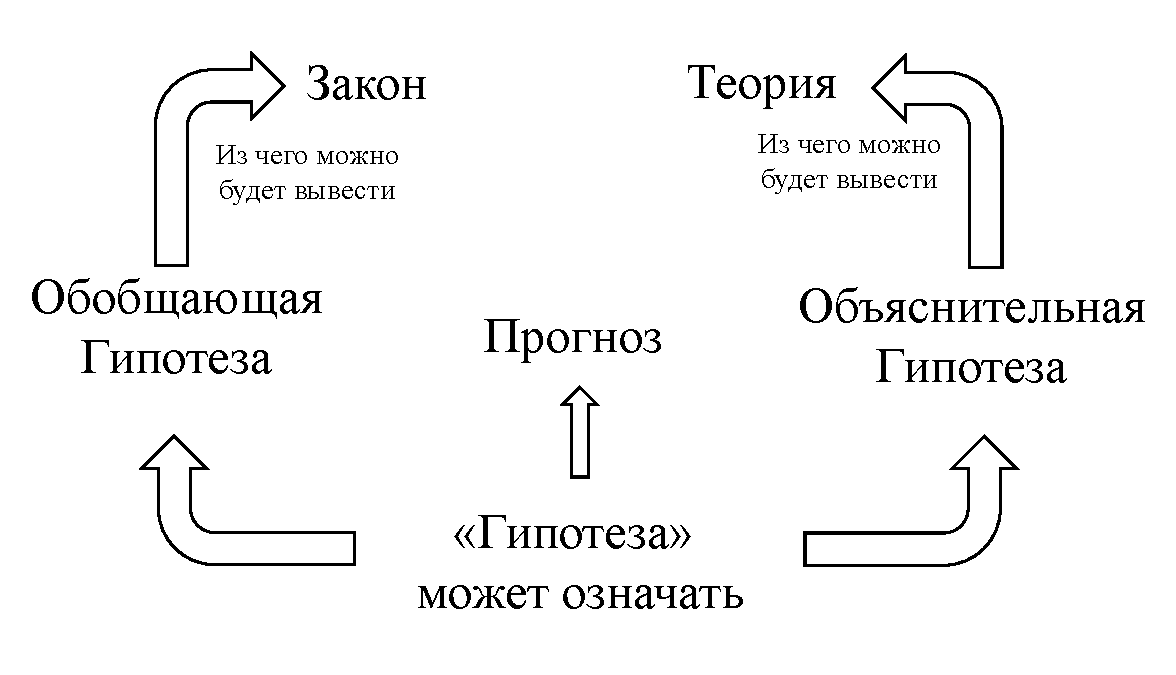
\includegraphics[width=0.7\linewidth]{images/hypothesis_life.pdf}
    \caption{Воплощение гипотезы.}\label{fig:hypothesis_repr}
\end{figure}

\textit{Научная гипотеза} есть предлагаемое объяснение явления, которое еще должно быть подвергнуто строгой проверке. 
В отличие от этого, \textit{научная теория} уже прошла всесторонние испытания и широко принята в качестве точного 
объяснения, стоящего за наблюдением. \textit{Научный закон} - это утверждение, которое показывает некоторую 
упорядоченность или регулярность в природе, \textit{существование неизменной связи между определенным комплексом 
условий и определенными явлениями}. В точных науках законы, как правило, выражаются в виде математических зависимостей. 
Гипотезы лежат в основе законов, а тщательно проверенные, подтвержденные гипотезы становятся теориями. В то же время 
законы не перестают быть законами, если они изначально не появились как гипотезы и не прошли стадию существования 
в качестве теорий.

Несмотря на то, что теории и законы являются разными видами знания, они все же представляют собой лишь разные формы 
одного и того же конструкта знания. Законы представляют собой обобщения, принципы или паттерны в природе, а теории 
разъясняют такие обобщения. Необходимо отметить, что классификация, представленная на ~\cref{fig:hypothesis_repr}, 
субъективна. Работа \cite{Rao1998} приводит примеры, показывающие, что различия между законами, гипотезами и теориями 
заключаются лишь в том, что они находятся на разных уровнях приемлемости – в зависимости от того, сколько накоплено 
эмпирических доказательств. Таким образом, нет существенного различия между конструктами, которые используются для 
выражения гипотез, теорий и законов. 

Едва ли можно переоценить важность роли гипотез в научных исследованиях. В издании книги А. Пуанкаре\cite{Poincare2015} 
подчеркнуто, что \textit{наука не существует без гипотез}. Поэтому неудивительно, что в научных исследованиях и 
соответствующих публикациях столь много внимания посвящено методам оперирования гипотезами с применением методов 
информатики в процессе экспериментального изучения и моделирования различных явлений. Мысль о том, что наукам, 
интенсивно использующим данные, и тем, которые опираются на гипотезы, необходимы новые подходы, пронизывает всю эту 
работу. Симбиоз такого рода, вместе с традицией науки, движимой гипотезами (<<сначала гипотеза, потом эксперимент>>), 
может привести также и к широкому применению другого метода исследований: <<сначала эксперимент, потом гипотеза>>. 
Во многих случаях порядок <<сначала эксперимент>> в ИИИД мотивируется необходимостью анализа существующих массивов 
данных с целью создания гипотезы. На \cref{fig:knowledge_production} показаны именно такие пути производства 
знаний~\cite{McComas2005}. <<Обобщение>> здесь означает любое подмножество гипотез, теорий и законов, 
а <<свидетельство>> "--- это любое подмножество всех фактов, накопленных в рамках конкретного ИИИД.

\begin{figure}[ht]
    \centering
    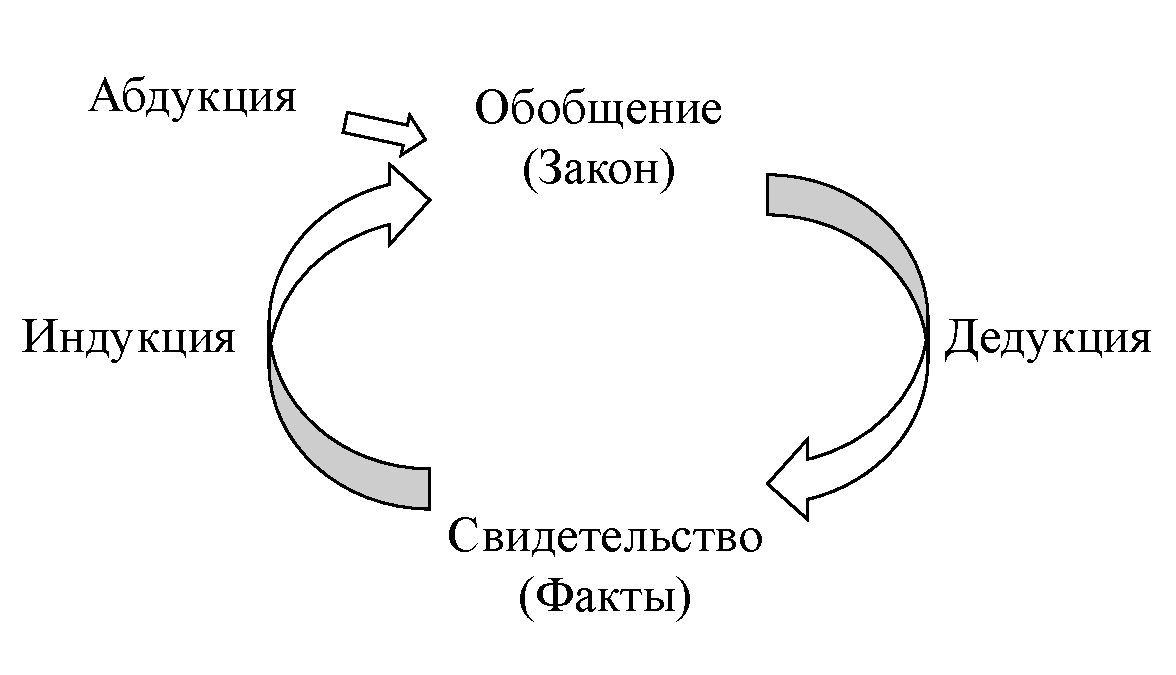
\includegraphics[width=0.7\linewidth]{images/science_lifecycle}
    \caption{Развернутая диаграмма производства знаний.}\label{fig:knowledge_production}
\end{figure}

Каждый исследователь занимается сбором и интерпретацией эмпирических доказательств; такой процесс называется индукцией. 
Это – методика, в которой собираются и рассматриваются разрозненные элементы доказательства до того момента, когда 
открывается закон или изобретается теория. Первым формализовал понятие индукции Ф.~Бэкон \cite{Bacon2000}. 
Предложенный им метод (наивной) индукции (\cref{fig:knowledge_production}) традиционно является основополагающим 
методом, с помощью которого человек, как правило, делал обобщения, позволяющие предсказывать события. Затруднения, 
связанные с индукцией, заключаются в том, что невозможно собрать воедино все наблюдения, касающиеся данной ситуации 
в любое время – в прошлом, настоящем и будущем.  

\textit{Закон} обобщает массу наблюдений. В целом, закон представляет собой группу связанных между собой неоспоримых 
гипотез, использующих небольшое количество фундаментальных понятий и уравнений, определяющих поведение некоторого 
множества явлений. Закон не является попыткой объяснить, <<почему так происходит>>, он просто констатирует факт. 
Формулирование нового закона начинается с индукции, когда факты наслаиваются на другие релевантные факты. А в целях 
проверки справедливости закона полезна дедукция.  На \cref{fig:knowledge_production} показано, что действительно 
справедливый закон всегда позволяет точное предсказание еще неизвестных фактов.  Кроме того, существует абдукция 
\cite{Menzies1996}, процесс проверки данной гипотезы путем последовательно аппроксимирующего логического рассуждения. 
Согласно этому принципу, всякое рассуждение справедливо, если оно является наилучшим объяснением данного множества 
известных данных. Абдуктивная валидация является общепринятой практикой формирования научных гипотез.

В \cite{Poincare2015} рассматриваются два рода используемых в науке гипотез: 

\begin{enumerate}
    \item Гипотезы, которые ценны именно потому, что они могут быть подтверждены или, напротив, опровергнуты путем 
        прямого обращения к тому, что предлагает опыт.
    \item Гипотезы, которые, несмотря на то, что опыт предполагает их, являются ценными, невзирая на то, или даже 
        вследствие того, что опыт не может ни подтвердить их, ни опровергнуть.
\end{enumerate}

Особенности науки, обуславливаемые использованием гипотез второго рода, рассматриваются А. Пуанкаре как «представляющий 
собой присущий человеку способ рассмотрения природы, интерпретацию, а не описание или предсказание объективных 
природных фактов, приспособление наших концепций внутренним потребностям нашего разума». По мнению А. Пуанкаре, 
центральной проблемой научной логики является проблема соотношения между двумя фундаментально разными видами гипотез, 
а именно между теми, которые не могут быть подтверждены или опровергнуты опытным путем, и теми, которые могут 
быть эмпирически проверены.

Любая полезная гипотеза позволяет прогнозирование посредством рассуждений (включая дедуктивные рассуждения). 
Она может предсказать исход эксперимента в лабораторных условиях или наблюдение природного явления. К прогнозированию 
также может привлекаться статистика при допущении, что гипотеза может быть опровергаемой \cite{Popper2005}, и что 
нельзя рассматривать предположение или теорию в качестве научных, если они не допускают самой возможности их 
несправедливости. Можно провести границу между гипотезами, если называть научными только те из них, для которых 
можно указать (заранее) одно или несколько потенциально опровергающих доказательств – таких, как соответствующие 
эксперименты. Опровержение предполагается дедуктивным, но не индуктивным.

Другие философы науки отвергают критерий опровергаемости или дополняли его другими критериями – например, критерием 
проверяемости (познавательно значимыми являются только такие утверждения относительно нашего мира, которые 
подтверждаются эмпирически или логически необходимы). Они утверждают, что наука движется в процессе 
<<индукции>> "--- т.е. путем поиска подтверждений предположениям (гипотезам). К.~Поппер считал, что подтверждения 
никогда не являются твердыми. Опровержение, однако, может оказаться неожиданным и определенным \cite{Popper2005}. 
А.~Эйнштейн высказался следующим образом: «Никакое количество экспериментов никогда не сможет доказать, что я прав; 
однако один"---единственный эксперимент сможет доказать, что я не прав». Для ученых и философов, не придерживающихся 
мнения К.~Поппера, наука работает, в основном, на базе индукции (подтверждения), а также, хотя и реже, на базе 
неподтверждения (опровержения). Языком науки почти всегда является язык индукции. В рамках данного обзора приемлемы 
оба философских подхода к гипотезам. Иногда такой способ рассуждения называется 
\textit{гипотетико"---дедуктивным методом}. В соответствии с этим методом научное исследование выполняется путем 
формулирования гипотезы в некоторой форме, которая предположительно могла бы быть опровергнута проверкой с помощью 
наблюдаемых данных. Проверка, которая могла бы противоречить и реально противоречит прогнозам гипотезы, признается 
опровержением гипотезы. Проверка, которая могла бы противоречить, но реально не противоречит прогнозам гипотезы, 
подтверждает данную теорию.

Научный метод включает в себя эксперимент, необходимый для проверки, может ли гипотеза дать адекватный ответ на 
поставленный вопрос. Прогноз на основе гипотезы предполагает проверку (наблюдение или эксперимент) гипотезы, которая 
таким образом и становится проверяемой. Если гипотеза не порождает возможность наблюдательной проверки, исследователь 
никак не может её использовать.

Например, можно выдвинуть непроверяемую гипотезу <<Наша вселенная погружена в другую, более масштабную вселенную, с 
которой мы не можем иметь абсолютно никакого контакта>>; вот потенциально подтверждаемая (хотя и потенциально 
проверяемая) гипотеза: <<Во вселенной есть другие обитаемые планеты>>; а вот научная гипотеза (проверяемая и 
подтверждаемая): <<Любые два предмета, сброшенные (одновременно) с одной и той же высоты над поверхностью земли, 
упадут на эту поверхность в один и тот же момент времени, если нет сопротивления воздуха>> \cite{Stanbrough2022}.

\textit{Задачу (научный вопрос)} следует формулировать в форме <<какое соотношение существует между двумя и 
более переменными>>. Постановка задачи должна быть такой, которая подразумевает возможности эмпирической 
проверки "--- в противном случае задача не будет научной. Задачи и гипотезы, будучи обобщенными формулировками 
соотношений, дают возможность делать вывод о конкретных эмпирических явлениях, подразумеваемых задачами и гипотезами. 
В такого рода процессе гипотезы могут быть выдвинуты на основе теории или других гипотез. Задача не может быть научно 
разрешена, если она не сведена к виду гипотезы, поскольку задача не может быть проверена 
непосредственно \cite{Azorin1966}.

\textit{Закон} обобщает массу наблюдений. В целом, закон представляет собой группу связанных между собой неоспоримых 
гипотез, использующих небольшое количество фундаментальных понятий и уравнений, определяющих поведение некоторого 
множества явлений. Закон не является попыткой объяснить, «почему так происходит», он просто констатирует факт.

Большинство формальных гипотез объединяют концепции, указывая на ожидаемые соотношения между \textit{предположениями}. 
Когда множество гипотез образует группу, они становятся \textit{концептуальной структурой}. Если концептуальная 
структура является комплексной и включает в себя каузальность или объяснение, её обычно называют 
\textit{теорией} \cite{Hempel1952}. Вообще говоря, гипотезы должны отражать многовариантную сложность реальности. 
\textit{Научная теория} обобщает гипотезу или группу гипотез, поддержанных неоднократными проверками. Теория 
справедлива, если нет ни одного противоречащего ей факта. \textit{Научная парадигма} объясняет рабочее множество 
теорий, на которых основана наука.

\section{Роль гипотез и моделей в исследованиях с интенсивным 
         использованием данных: фундаментальные принципы}\label{sect1_2}

\subsection{Различные представления научных гипотез}\label{sect1_2_1}
Существует множество представлений научных гипотез в исследованиях 
с интенсивным использованием данных (см. \cref{fig:hypothesis_representation}).

\begin{figure}[ht]
    \centering
    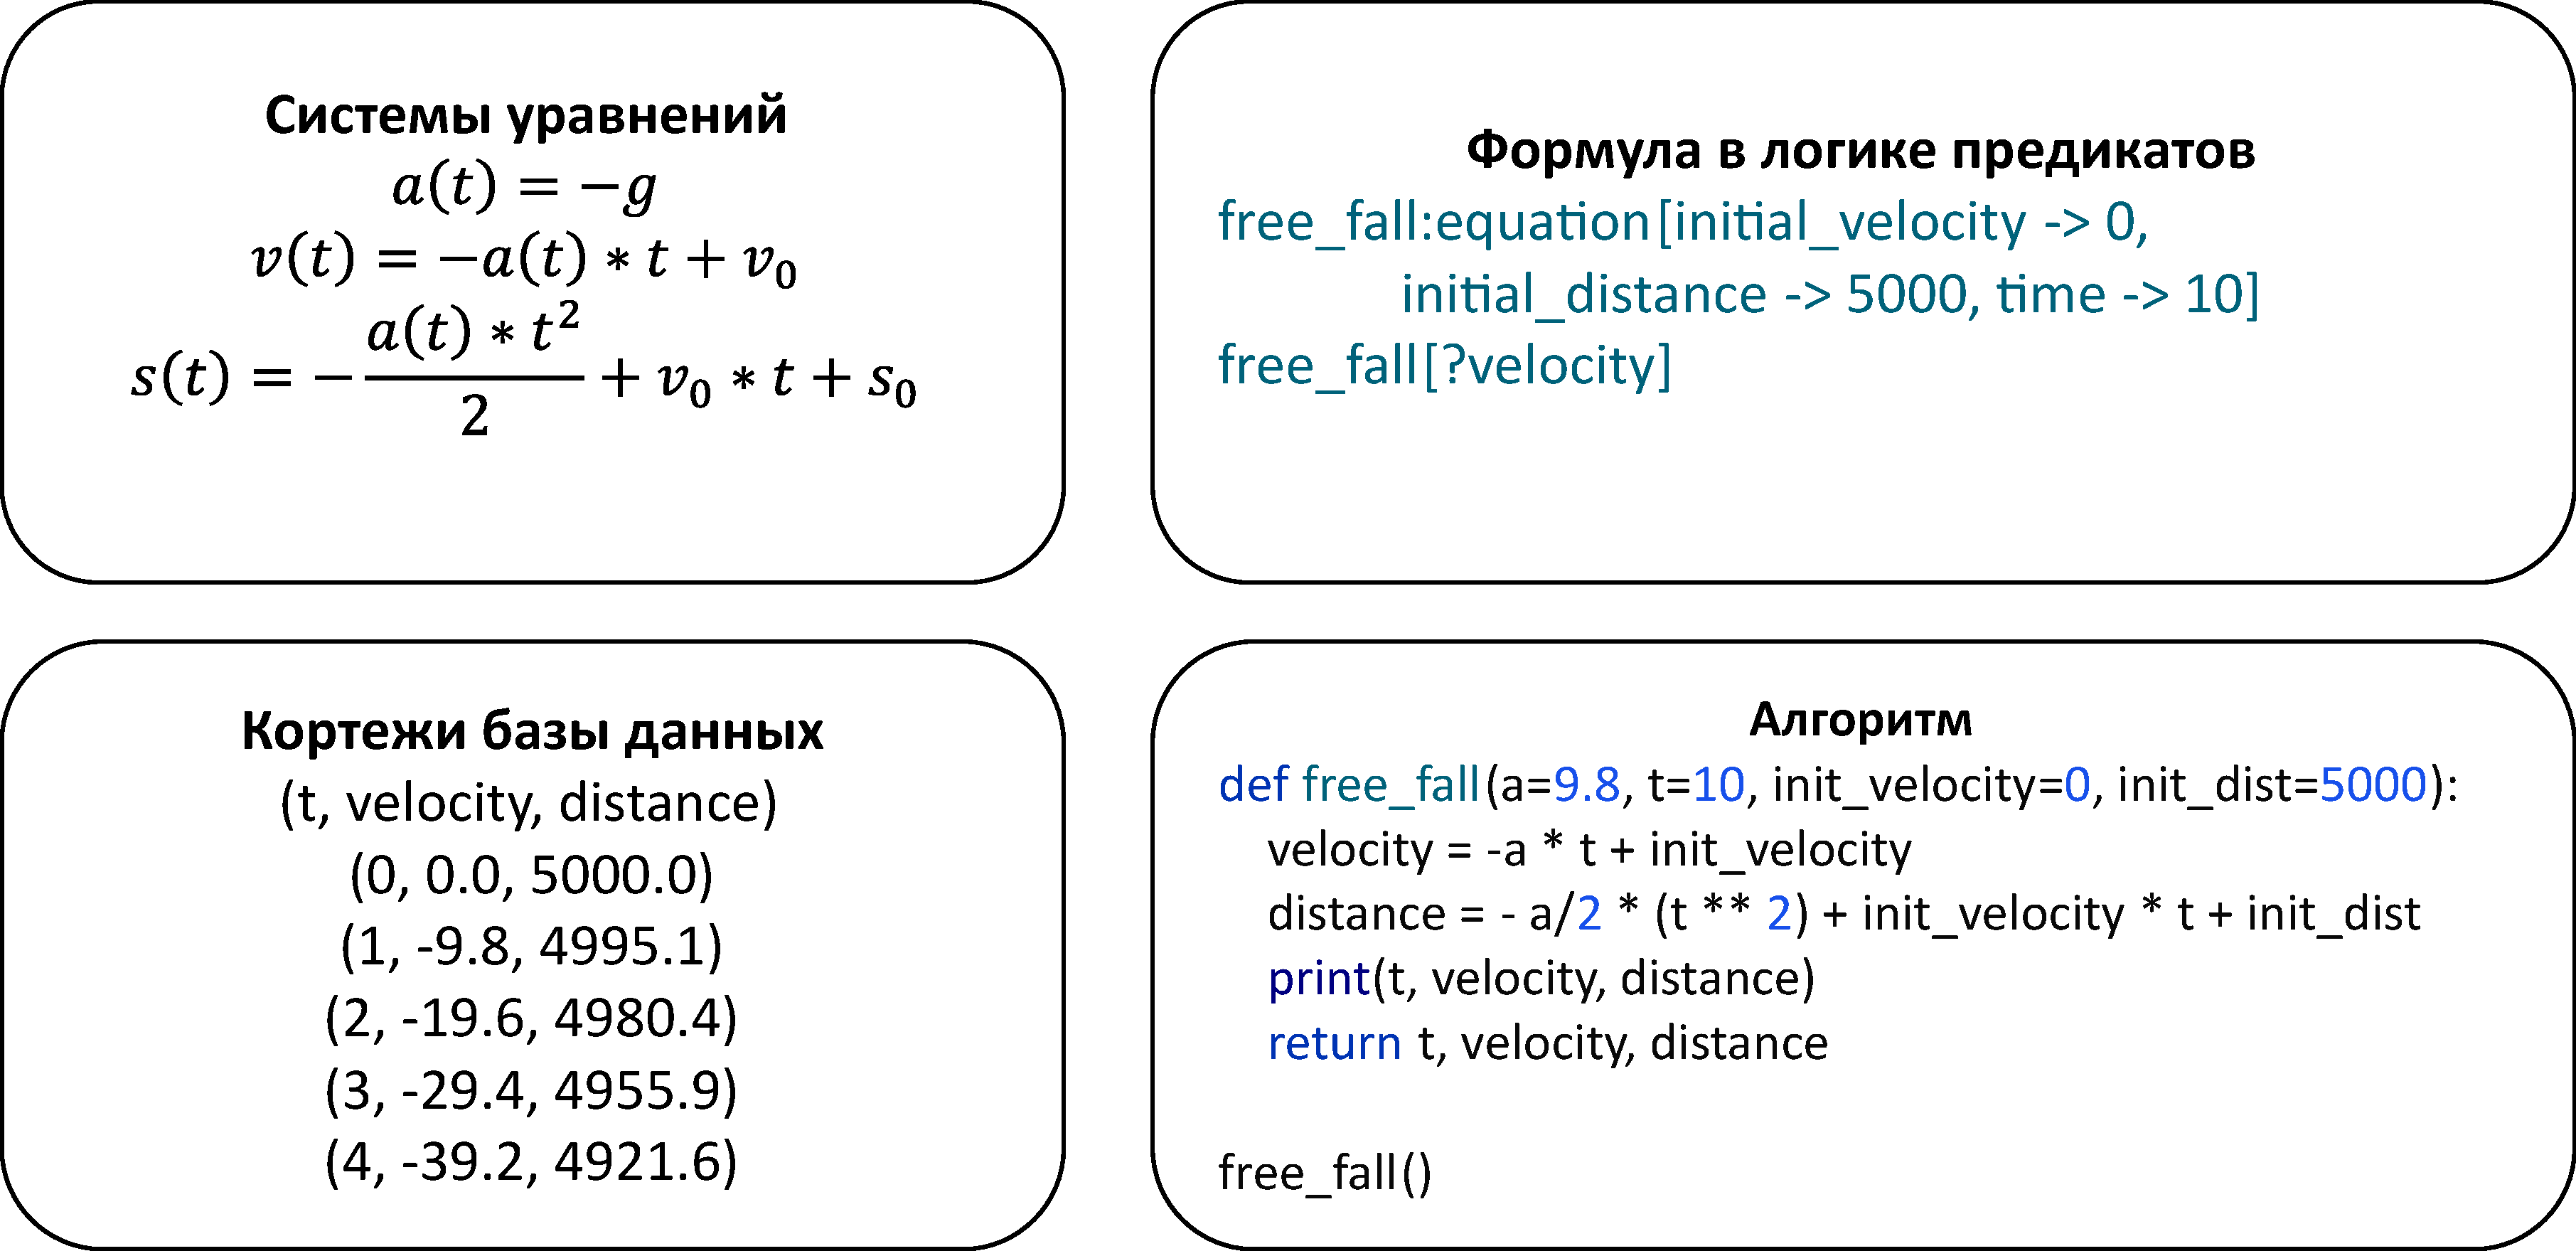
\includegraphics[width=1.0\linewidth]{images/hypothesis_representation.pdf}
    \caption{Различные представления научных гипотез.}\label{fig:hypothesis_representation}
\end{figure}

Например, научные гипотезы имеют вид математической модели. Иногда их также можно формулировать как предложения в 
логике предикатов, констатирующие, что в определенном случае рассматриваемое явление обладает некоторой 
характеристикой, а также каузальные утверждения, имеющие общую форму универсальных утверждений, 
констатирующих, что явление во всех случаях имеет определенную характеристику (напр., для всех x, если 
x "--- лебедь, то x "--- белый). Научная гипотеза, рассматриваемая как декларативное утверждение, указывает 
прогнозируемое соотношение (ассоциативное или каузальное) между двумя или более переменными (зависимыми или 
независимыми и зависимыми). В случае каузального соотношения изменение, имеющее своей причиной независимую переменную, 
прогнозируется зависимой переменной. Переменные чаще всего связаны некаузально (ассоциативно) \cite{Haber2009}.

В экспериментальных работах исследователь манипулирует независимой переменной. Зависимую переменную часто считают 
следствием или предполагаемым результатом, который изменяется вслед за изменением независимой переменной. Зависимой 
переменной не манипулируют. Она наблюдается и принимается в качестве изменяющейся с изменением независимой переменной. 
Прогнозирование делается в направлении от независимой переменной к зависимой переменной. Исследователя интересует 
понимание, объяснение или прогнозирование именно зависимой переменной \cite{Haber2009}.

В том случае, когда исследуется возможная корреляция или подобное соотношение между переменными (как, например, 
является ли предлагаемый препарат эффективным в лечении болезни, т.е., по крайней мере, до некоторой степени и для 
некоторых пациентов), немногочисленные случаи, где испытываемое лекарство не дает результата, не опровергают гипотезу. 
На самом деле, для определения того, насколько вероятно, что общий эффект будет наблюдаться, если не существует 
реального соотношения, заложенного в гипотезе, используются статистические испытания. Если такая вероятность достаточно 
мала, существование некоторого соотношения может быть допущено. При статистическом испытании гипотез сравниваются две 
гипотезы, называемые нулевой гипотезой и альтернативной гипотезой. Нулевая гипотеза утверждает, что нет соотношения 
между исследуемыми явлениями (переменными), или, по крайней мере, его нет в форме, предлагаемой альтернативной 
гипотезы. Альтернативная гипотеза, как и предполагает её наименование, это альтернатива нулевой гипотезы: она содержит 
утверждение, что некоторое соотношение существует.

Альтернативные гипотезы, как правило, используются чаще, чем нулевые, поскольку они более желательны для реализации 
ожиданий исследователя. Однако в любом исследовании, использующем статистический анализ, как правило, всё же 
допускается лежащая в основе нулевая гипотеза \cite{Haber2009}. Здесь важно то, что положение «не отвергайте нулевую 
гипотезу» необязательно означает, что нулевая гипотеза справедлива. Оно лишь предполагает, что нет существенных 
доказательств в пользу альтернативной гипотезы в противовес нулевой гипотезы. Отбрасывание же нулевой гипотезы 
предполагает, что альтернативная гипотеза может оказаться справедливой.

Элементы движимых гипотезами исследований и их соотношения показаны на \cref{fig:hypothesis_real} 
\cite{Goncalves2013, Porto2011}. Соотношения треугольника гипотезы (\textit{объясняет, формулирует, представляет}) 
конструктивны для принятия исследователем окончательного решения: выбрать конкретную модель $m_i$ с целью 
формулирования гипотезы $h_i$, которая предназначена для объяснения явления $p_i$. 

\begin{figure}[ht]
    \centering
    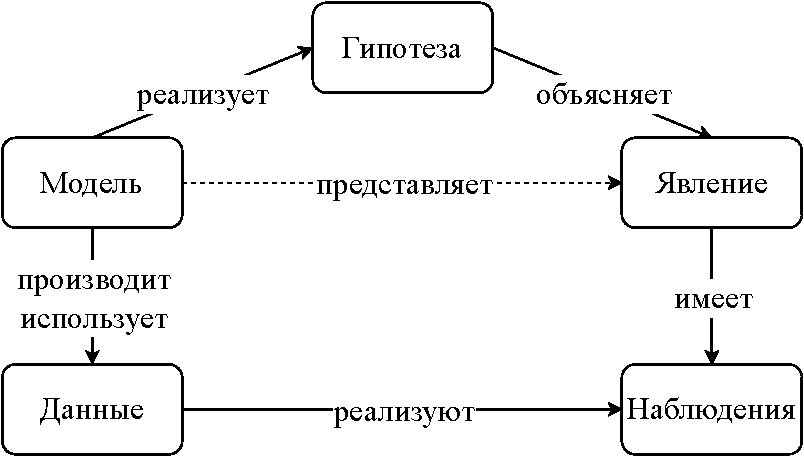
\includegraphics[width=0.7\linewidth]{images/hypothesis_real}
    \caption{Элементы движимых гипотезами исследований.}\label{fig:hypothesis_real}
\end{figure}

В работе \cite{Goncalves2013} предлагается решетчатая структура соединения гипотез, как показано на 
\cref{fig:hypothesis_relation}. Решетка гипотез образуется при рассмотрении множества гипотез, расположенных 
в строгом порядке \textit{derived\textunderscore by} "--- была выведена из (снизу вверх). Гипотезы, 
непосредственно выведенные из одной единственной гипотезы, называются атомарными, в то время как те, которые выведены, 
по крайней мере, из двух гипотез, называются комплексными.

\begin{figure}[ht]
    \centering
    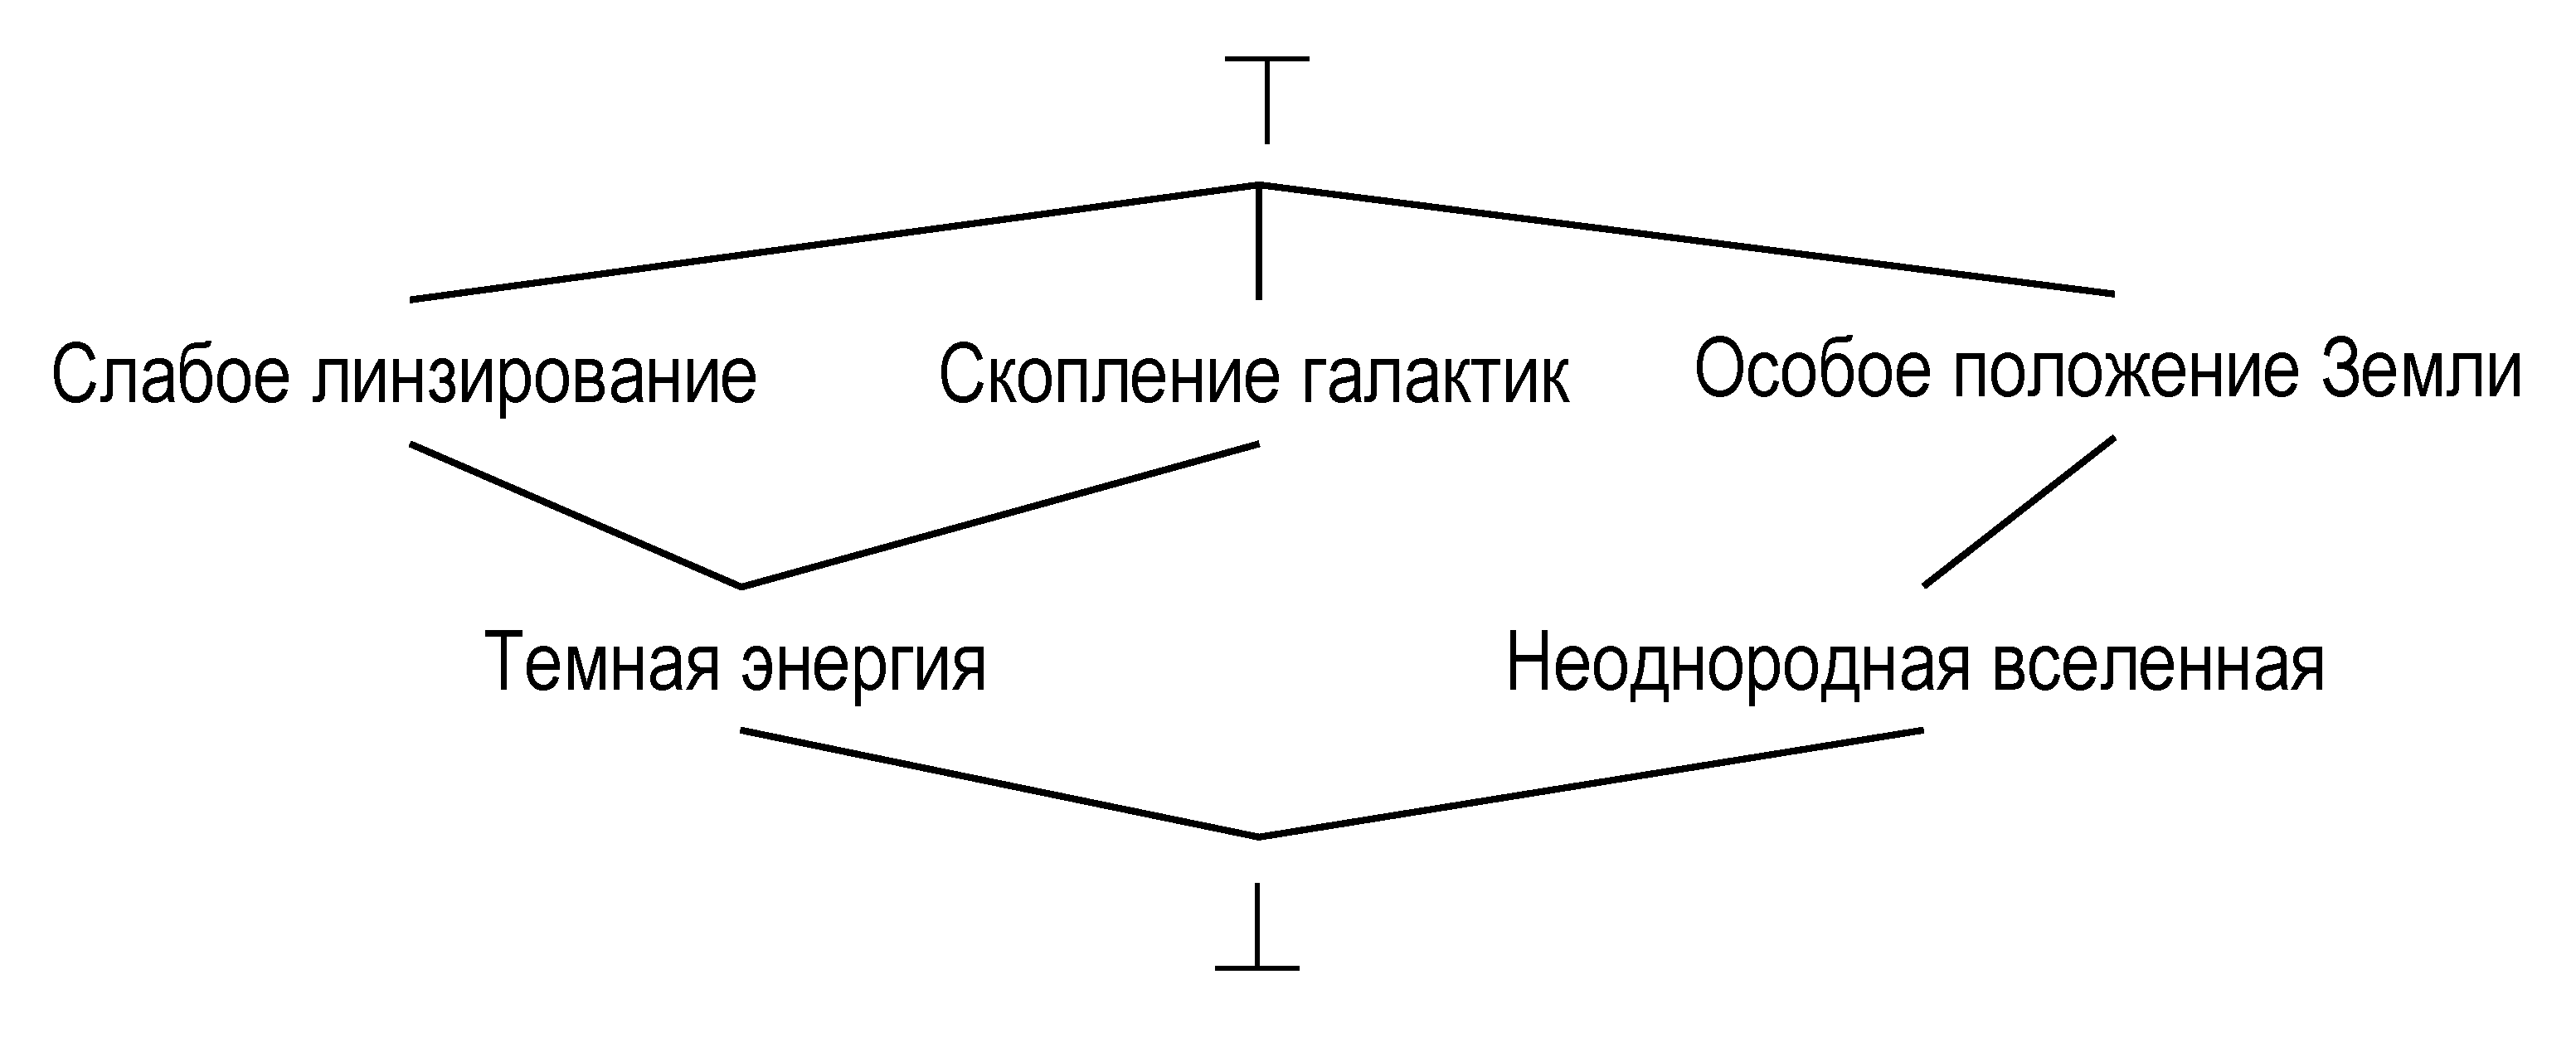
\includegraphics[width=0.7\linewidth]{images/hypothesis_relation.pdf}
    \caption{Теоретическое представление отношений в решетке гипотез.}\label{fig:hypothesis_relation}
\end{figure}

Решетка гипотез разворачивается в модель и изоморфные решетки явлений в соответствии с треугольником 
гипотез \cref{fig:hypothesis_real}. Решетки изоморфны, если исследователь выбирает такие подмножества $M$ (моделей), 
$H$ (гипотез) и $P$ (явление) так, что они формулируют, объясняют и представляют как один в один, так и отображения 
на себя (т.е. взаимно-однозначные соответствия), рассматриваемые как отображения, сохраняющие структуру (морфизмы). 
Пример изоморфной решетки показан на \cref{fig:lattice_fluid}. Эта решетка соответствует случаю в вычислительной 
гемодинамике, рассмотренному в \cite{Goncalves2013}. Здесь модель $m_1$ формулирует гипотезу $h_1$, которая объясняет 
явление $p_1$. Подобным же образом модель $m_2$ формулирует $h_2$, которая объясняет $p_2$, и т.д. Свойства решеток 
гипотез и операции с ними рассматриваются в \cite{Goncalves2012}.

\begin{figure}[ht]
    \centering
    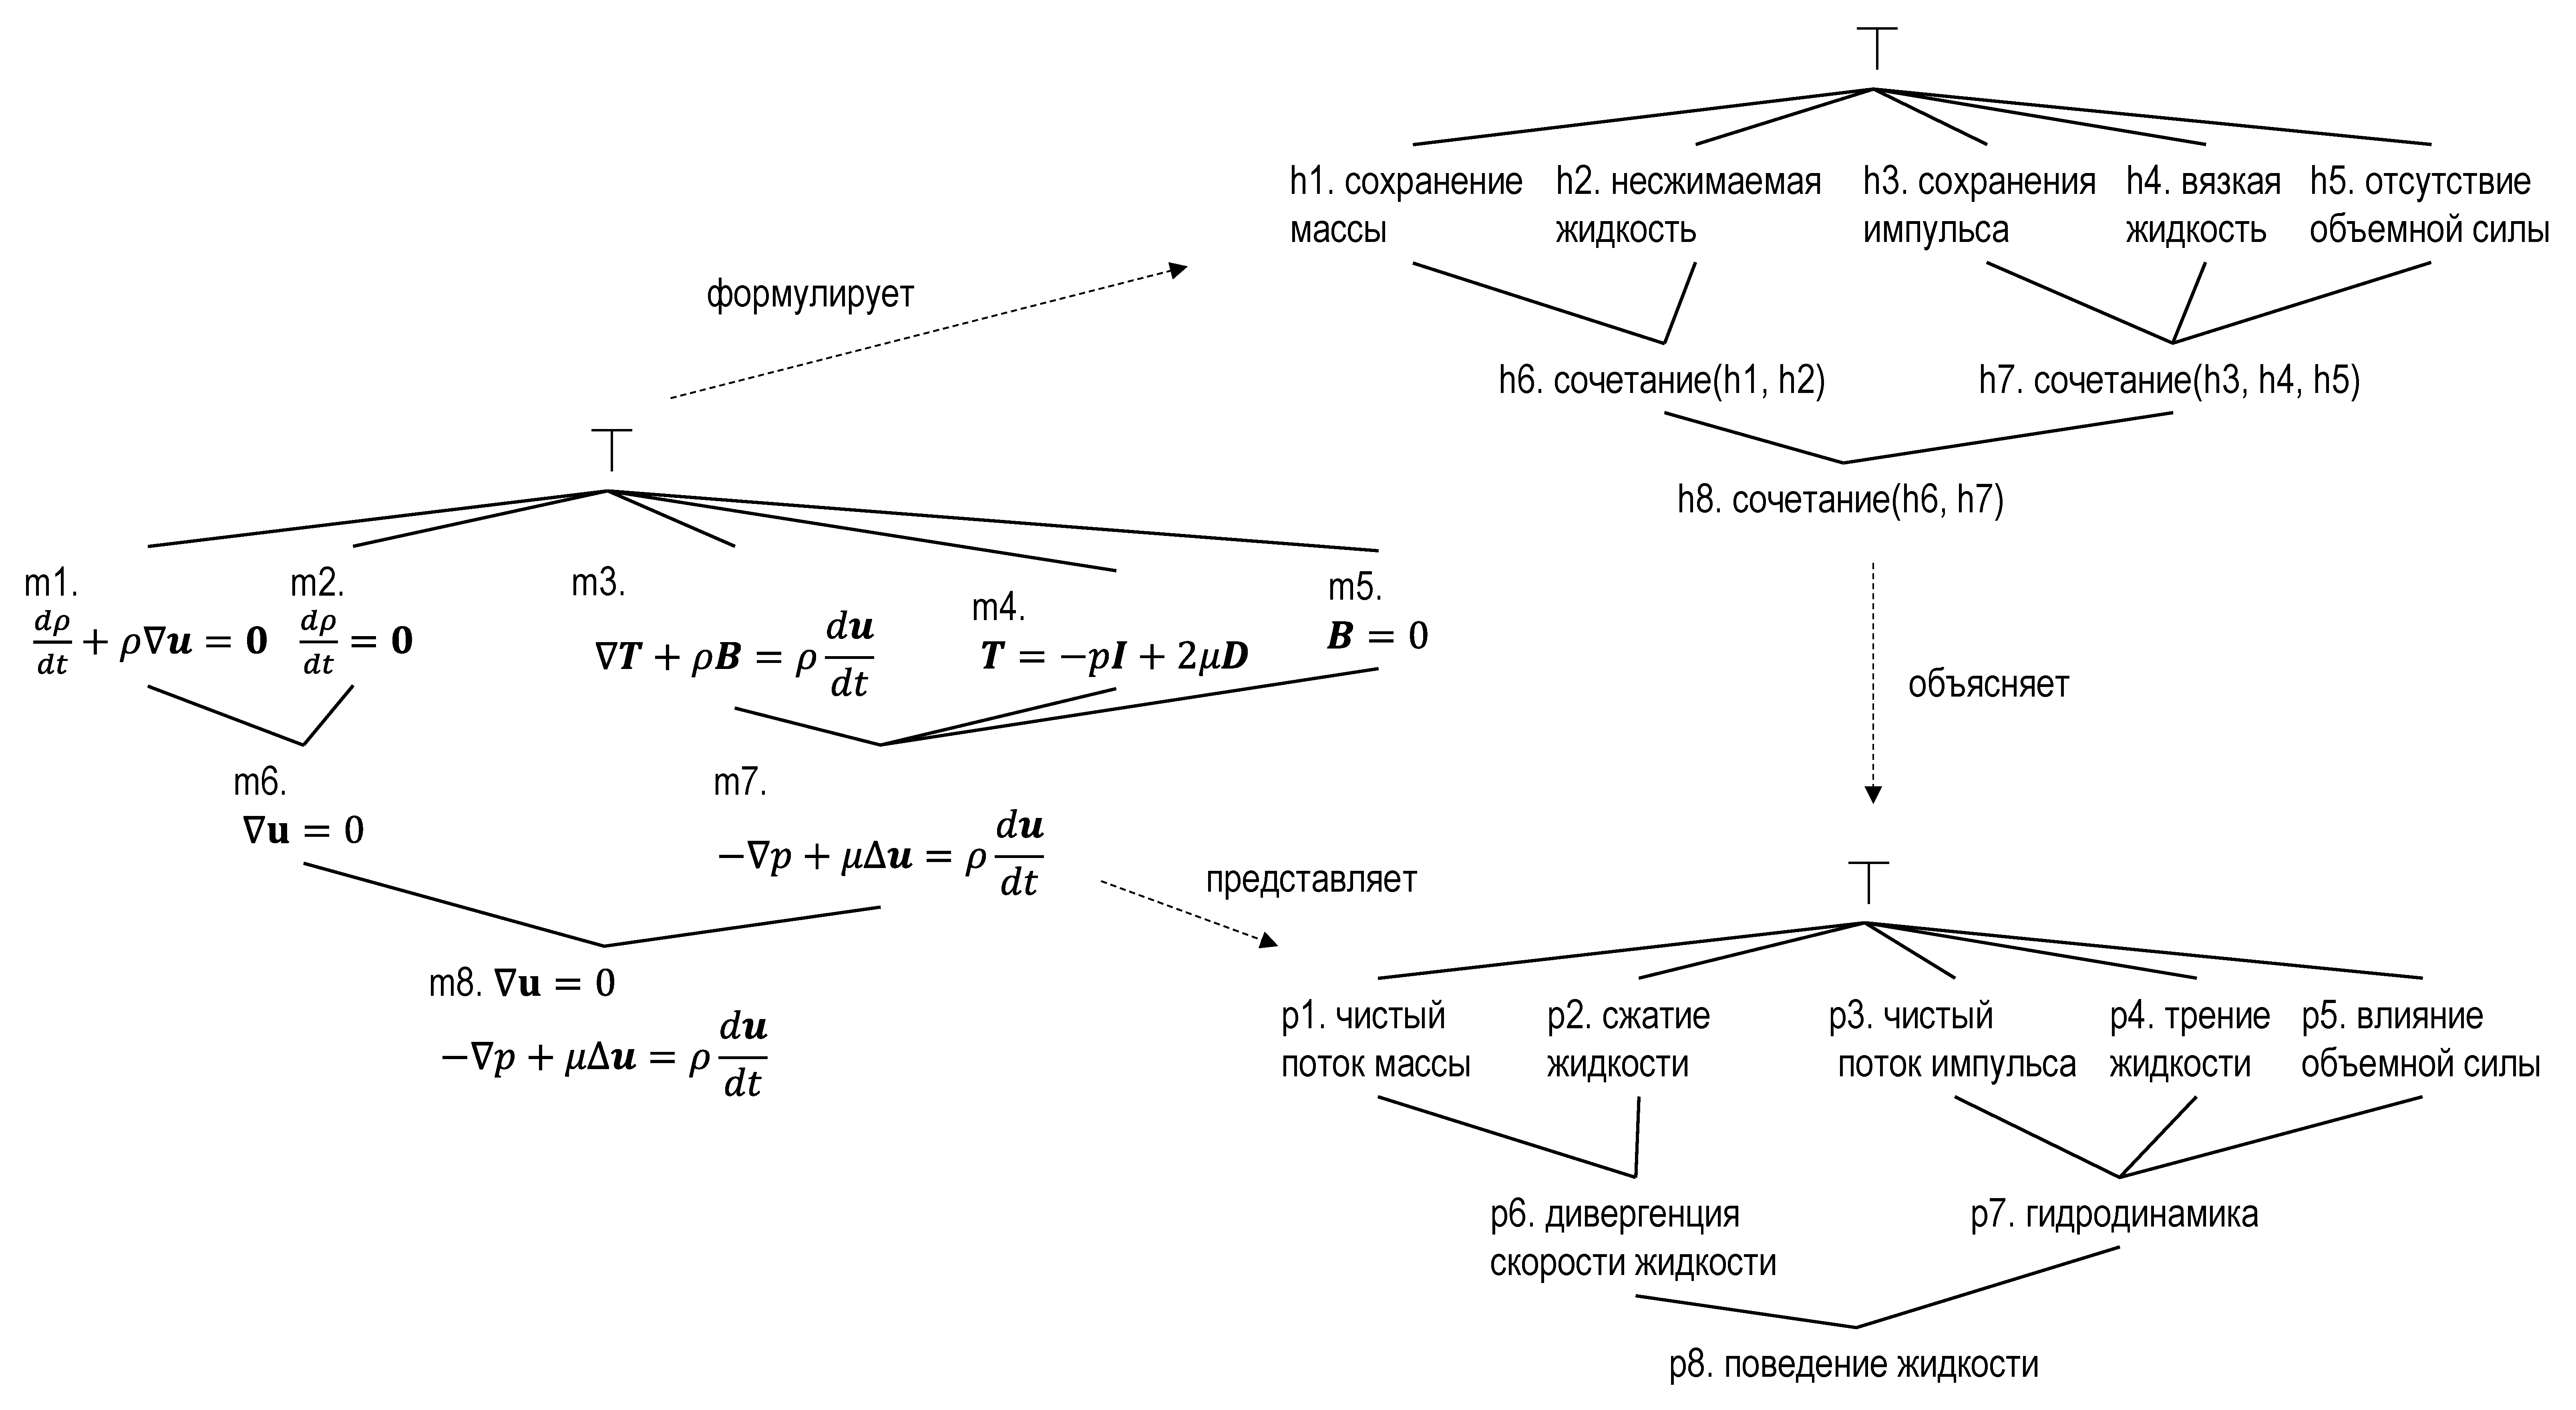
\includegraphics[width=1.0\linewidth]{images/lattice_fluid.pdf}
    \caption{Решетка гипотез, развернутая в модель, и изоморфная решётка явлений.}\label{fig:lattice_fluid}
\end{figure}

\textit{Модели} являются одним из основных инструментов современной науки. Модели могут выполнять две принципиально 
различные функции представления: модель может быть представлением выделенной части мира, или же модель может 
представлять определенную теорию в том смысле, как она (модель) интерпретирует законы и гипотезы данной теории.

Один из наиболее трудных вопросов в связи с моделями "--- это как они соотносятся с теориями. В этом плане модели 
могут рассматриваться как дополнения к теориям, как предварительные теории; они могут быть использованы в качестве 
замены теории, если теория слишком сложна для работы. Изучение модели ведется посредством прямых экспериментов, 
мысленных экспериментов и симуляции. Если задан набор параметров, модель может генерировать предполагаемые результаты 
относительно того, как система будет вести себя в конкретной ситуации. Модель и гипотезы, на которых она основана, 
укрепляются, если модель генерирует результаты, которые соответствуют поведению своего прототипа в реальном мире. 

\subsection{Проверка гипотез}\label{sect1_2_2}
Если научная гипотеза может быть проверена и опровергнута, она становится хорошей основой для дальнейшего 
моделирования. Для этого есть несколько способов, включая использование статистики, байесовского и логического вывода.
\subsubsection{Статистическая проверка гипотез}\label{sect1_2_2_1}
Для проверки и отбора гипотез применим как классический (частотный), так и байесовский статистический подход. 
Краткое изложение основных различий между этими подходами приведено ниже \cite{ivezic2019statistics}.

Классическая (частотная) статистика основана на следующих представлениях:
\begin{itemize}
    \item Вероятности "--- это относительные частоты событий. Они являются объективными свойствами объективного мира.
    \item Параметры гипотез (модели) являются фиксированными неизвестными константами. Поскольку они неизменны, 
            вероятностные утверждения относительно параметров не имеют смысла.
    \item Методы статистики должны иметь точно определенные долгосрочные частотные свойства.
\end{itemize}

После того как сформулированы нулевая и альтернативная гипотезы, необходимо принять некоторые статистические допущения 
относительно выборок данных, например, допущения о статистической независимости или распределения наблюдений. Если 
корректные допущения не приняты, это приводит к неверным результатам проверки.

Общая задача классической статистики "--- это задаться вопросом, согласуется ли данная выборка с гипотезой. Например, 
нас может интересовать, является ли результат измерения $x_i$ или даже целое множество $\{x_i\}$ согласуется с тем, 
что было выбрано из гауссова распределения $\mathcal{N}(\mu,\,\sigma^{2})$. Это \textit{нулевая гипотеза}.

Всегда принимается, что нам известно, как вычислить вероятность данного исхода на основе нулевой гипотезы: например, 
дана кумулятивная функция распределения, $0 \leq H_0(x) \leq 1$, тогда вероятность, что мы получим значение, 
по крайней мере, такое, как $x_i$, будет $p(x > x_i) = 1 $ "--- $H_0(x_i)$, и оно называется 
\textit{достигаемым уровнем значимости} $p$. Обычно принимается некоторый порог значения $p$, 
называемый \textit{уровнем значимости} $\alpha$, и нулевая гипотеза отвергается, если $p \leq \alpha $ 
(например, если $\alpha = 0.05$ и $p < 0.05$, нулевая гипотеза отвергается при уровне значимости $0.05$). 
Если мы не отвергаем гипотезу, это не означает, что её корректность доказана, поскольку может оказаться, что объем 
выборки просто недостаточно велик для получения результата.

При выполнении такого рода проверок можно столкнуться с ошибками двух типов; статистики называют их 
\textit{ошибки I и II рода}. Ошибки I рода "--- это случаи, когда нулевая гипотеза верна, но несправедливо 
отвергнута. Применительно к поиску источников источники таких ошибок ложные, или, в более общем плане, такие 
результаты являются ложноположительными (в отношении альтернативной гипотезы). Вероятность ложноположительного 
результата при проверке единственного значения ограничивается принятым уровнем значимости $\alpha$. Случаи, когда 
нулевая гипотеза несправедлива, но не отвергается, называются ошибками II рода (недостаточные источники, или 
ложноотрицательные результаты (опять же в отношении альтернативной гипотезы)). Вероятность ложноотрицательного 
результата при проверке единственного значения обычно обозначается как $\beta$, и она связана с 
\textit{мощностью критерия} как $(1-\beta)$. Проверка гипотез тесно связана со сравнением распределений.

Если понизить уровень значимости $\alpha$ (критерий отбрасывания нулевой гипотезы становится более консервативным), 
количество ложноположительных результатов уменьшится, а количество ложноотрицательных увеличится. Таким образом, 
необходим компромисс, чтобы найти оптимальное значение $\alpha$, которое зависит от относительной важности 
ложноотрицательных и ложноположительных результатов для конкретной задачи. И одобрение ложных гипотез, и отбрасывание 
справедливых гипотез являются ошибками, которые исследователи должны стараться избегать. Существует дискуссия о том, 
какой случай \textit{менее} желателен; многие полагают, что всегда хуже, чем непринятие справедливой, и что наука 
должна в первую очередь стремиться избегать принятия ложных гипотез.

Если выполняется много случаев проверки гипотезы (такой процесс называется \textit{множественной проверкой гипотез}), 
доля ложноположительных результатов может существенно превысить значение $\alpha$. Доля ложноположительных результатов 
зависит не только от $\alpha$ и количества значений, но также и от количества справедливо положительных результатов 
(последнее пропорционально количеству случаев, когда альтернативная гипотеза справедлива). 

В зависимости от вида данных (дискретные или непрерывные случайные переменные), от того, что можно допустить (или нет) 
относительно лежащих в основе распределений, а также от конкретно поставленного вопроса, можно воспользоваться 
различными статистическими проверками. Исходная идея статистических тестов заключается в использовании данных для 
расчета надлежащей статистики и последующего сравнения полученного на основе данных значения с его ожидаемым 
распределением. Ожидаемое распределение оценивается \textit{в предположении, что нулевая гипотеза справедлива}. 
Если такое ожидаемое распределение подразумевает маловероятность того, что полученное на основе данных значение 
возникло случайно (т.е., соответствующее значение $p$ мало), то нулевая гипотеза отвергается с учетом пороговой 
вероятности $\alpha$, обычно 0.05 или 0.01 $(p < \alpha)$. Заметим еще раз, что $(p \geq \alpha)$ не означает 
\textit{доказанности} гипотезы.

Количество различных статистических тестов в литературе очень велико, и часто бывает трудно оценить их применимость 
(см. \cite{field2013discovering, wagner2019using}) в отношении разнообразия статистических методов в пакете 
статистических методов для социальных наук (Statistical Package for the Social Sciences "--- SPSS). Если распределения 
неизвестны, такие тесты называются непараметрическими. Наиболее популярным является тест Колмогорова-Смирнова, где 
проводится сравнение кумулятивного распределения функции $F(x)$ для двух выборок $\{x_{1i}\}, i = 1, \ldots, N_1$ и 
$\{x_{2j}\}, j = 1, \ldots, N_2$. Тест Колмогорова-Смирнова не является единственным вариантом для непараметрического 
сравнения распределений. Критерий Крамера–фон Мизеса, тест Ватсона и тест Андерсона-Дарлинга сходны с тестом 
Колмогорова-Смирнова, хотя и рассматривают несколько иную статистику. Тест Манна–Уитни–Вилкоксона (или критерий 
суммы рангов Вилкоксона) "--- непараметрический критерий для проверки того, получены ли два множества данных из 
распределений с разными параметрами положения (если известно, что эти распределения гауссовы, стандартный классический 
тест называется t-тестом). Можно воспользоваться несколькими стандартными классическими тестами, если известно или 
можно допустить, что $h(x)$ и $f(x)$ – гауссовы распределения (например, тест Андерсона–Дарлинга, тест Шапиро–Уилка). 
Дальнейшую информацию по статистическим тестам можно найти в \cite{ivezic2019statistics, field2013discovering, 
wagner2019using}.

\subsubsection{Выбор гипотезы (модели) и проверка в байесовском стиле}\label{sect1_2_2_2}

В отличие от частотного, байесовский подход принимает следующие допущения:
\begin{itemize}
    \item Вероятность указывает на степень субъективного убеждения, не ограниченного частотностью. Вероятностные 
        утверждения могут относиться не только к данным, но и к другим вещам, включая сами гипотезы (модели), а также к 
        их параметрам.
    \item Выводы относительно параметра делаются на основе его распределения вероятностей "--- такое распределение 
        дает количественную оценку неопределенности нашего знания относительно данного параметра. Различные точечные 
        оценки, как, например, математическое ожидание, могут быть затем легко получены из этого распределения.
\end{itemize}

Байесовская интерпретация вероятностей может рассматриваться как расширение логики высказываний (пропозиционной 
логики), которая позволяет рассуждения посредством гипотез, т.е. высказываний, чья справедливость или несправедливость 
не определены.

Байесовская вероятность относится к категории доказательственных вероятностей; чтобы оценить вероятность гипотезы, 
приверженец байесовской вероятности указывает некоторую априорную вероятность, которая впоследствии обновляется в 
свете новых релевантных данных (фактов) \cite{sivia2006data}. Байесовская интерпретация предоставляет стандартный 
набор методов и формул для выполнения таких расчетов.

Байесовский подход может рассматриваться как формализация процесса постоянного уточнения нашего знания об окружающем 
мире, начиная с отсутствия данных (состояние \textit{a priori}), и последующего совершенствования знания, умножая 
его вероятность по мере наблюдения данных в целях получения знания \textit{a posteriori}. Если рассматривается еще 
больший объем данных, то полученные из опыта апостериорные данные, основанные на первичном множестве данных, могут 
быть использованы в качестве априорных для вторичного анализа. Конечно, множества данных могут быть различными.

Нередко возникает вопрос: какую «наилучшую» модель (гипотезу) использовать? \textit{<<Выбор модели>>} "--- это 
методика, которой можно воспользоваться с целью провести грань между конкурирующими моделями (гипотезами) и выделить 
наилучшую модель (гипотезу) из некоторого множества ${M_1,\ldots, M_n}$, если есть определенные данные.

Необходимо напомнить базовую систему обозначений. Теорема Байеса может быть использована для расчета апостериорной 
вероятности $p(M_j|d)$ для каждой модели (или гипотезы) $M_j$, представляющей состояние нашего знания относительно 
справедливости модели (гипотезы) в свете данных $d$:

\begin{equation}
p(M_j|d) = \frac{p(d|M_j)p(M_j)}{p(d)} 
\end{equation}
где $p(M_j)$ "--- априорное понимание модели (гипотезы), которая представляет состояние нашего знания (или незнания) 
о справедливости модели (гипотезы) до начала анализа текущих данных, $p(d|Mj)$ "--- \textit{правдоподобность} модели 
(гипотезы), представляющая вероятность, что некоторые данные будут получены при допущении данной модели, 
и $p(d)$ "--- константа нормализации:

\begin{equation}
p(d) = \sum_{i} p\left( d|M_i\right) p(M_i)  
\end{equation}

Относительная «приемлемость» моделей получается сравнением апостериорных вероятностей; поэтому для сравнения двух 
моделей $M_a$ и $M_b$ мы рассматриваем отношение между апостериорными вероятностями моделей:

\begin{equation}
\frac{p(M_a|d)}{p(M_b|d)} = \frac{p(d|M_a)p(M_a)}{p(d|M_b)p(M_b)} 
\end{equation}

Коэффициент Байеса $B_{ab}$ может быть рассчитан как отношение правдоподобностей моделей:

\begin{equation}
B_{ab} = \frac{p(d|M_a)}{p(d|M_b)}
\end{equation}

Эмпирическая шкала на основе коэффициента Байеса $B_{ij}$ для оценки силы доказательств по двум моделям показана 
в \cref{tbl:bayescoef} \cite{march2011should}.

\begin{table} [ht]%
	\caption{Сила доказательств по двум моделям на основе коэффициента Байеса $B_{ij}$}%
	\label{tbl:bayescoef}% label всегда желательно идти после caption
    \setlength\extrarowheight{0pt} %вот этим управляем расстоянием между рядами, \arraystretch даёт неудачный результат
    \setlength{\tymin}{2.3cm}% минимальная ширина столбца
    \begin{center}

	\begin{tabulary}{\textwidth}{@{}>{\zz}C >{\zz}C >{\zz}L@{}}% Вертикальные полосы не используются принципиально, 
        % как и лишние горизонтальные (допускается по ГОСТ 2.105 пункт 4.4.5) % @{} позволяет прижиматься к краям
        \toprule     %%% верхняя линейка
    	$ |\ln B_{ij}| $ &
    	Соотношение ($\nu$) &
    	Мощность доказательства	\\
        \midrule %%% тонкий разделитель. Отделяет названия столбцов. Обязателен по ГОСТ 2.105 пункт 4.4.5 
        $<1.0$ &
        $<3:1$  &
        Недостаточное доказательство 
        \\
        \midrule
        $ 1.0 $ &
        $ ~3:1 $  &
        Слабое  доказательство 
        \\
        \midrule
        $2.5$ &
        $~12:1$  &
        Доказательство средней силы 
        \\
        \midrule
        $5.0$ &
        $~150:1$  &
        Сильное доказательство 
        \\
        \bottomrule %%% нижняя линейка
	\end{tabulary}%
 \end{center}
\end{table}

Коэффициент Байеса предлагает меру «приемлемости» модели независимо от более раннего представления о модели; 
чем больше коэффициент Байеса, тем лучше модель. Во многих случаях предварительное представление о каждой модели 
множества предлагаемых моделей будет одинаковым, тогда коэффициент Байеса будет эквивалентен соотношению апостериорных 
вероятностей моделей. «Наилучшая» модель в байесовском смысле "--- это та модель, которая наилучшим образом 
согласуется с данными в наименьшем параметрическом пространстве.

Особым случаем выбора модели (гипотезы) является \textit{байесовская проверка гипотезы} 
\cite{ivezic2019statistics, rouder2009bayesian}. Приняв $M_1$ как «нулевую» гипотезу, можно поставить вопрос: 
поддерживают ли данные альтернативную гипотезу $M_2$, т.е., можно ли отвергнуть нулевую гипотезу. Принимая априорные 
вероятности $p(M_1) = p(M_2)$ равными, получим отношение вероятностей

\begin{equation}
B_{21} = \frac{p(d|M_1)}{p(d|M_2)}  
\end{equation}

Невозможность отвергнуть $M_1$ в отсутствие альтернативной гипотезы весьма отлично от ситуации в процедуре проверки 
гипотезы в классической статистике. Последняя процедура отвергает нулевую гипотезу, если она не дает правильного 
описания данных, т.е. если очень маловероятно, что имеющиеся данные могут быть сгенерированы так, как предписывает 
нулевая гипотеза. Напротив, байесовский подход основан не на апостериорной вероятности данных, а на их апостериорной 
правдоподобности (вероятности), и не может отвергнуть гипотезу, если нет альтернативных объяснений наблюдаемых данных.

Сравнивая классический и байесовский подходы \cite{ivezic2019statistics}, трудно ожидать, что критически важный анализ 
будет выполнен в «абсолютно байесовском» стиле, т.е. без использования на разных стадиях частотных инструментов на 
разных стадиях процесса. Оставляя в стороне философию и красоту, можно сказать, что надежность вероятность и 
эффективность соответствующих вычислений при реализации байесовского подхода являются главными практическими вопросами. 
Центральным техническим вопросом, занимающим здесь основное место, является то, что значительно легче выполнить 
оптимизацию (надежно и эффективно) в больших размерностях, чем выполнить интегрирование. Так, используемые методы 
машинного обучения, хотя и прилагаются усилия адаптировать их к байесовской концепции, почти все основаны на 
частотных методах. 

Большинство из тех, кто применяет методы байесовской оценки, склонны на практике комплексно использовать байесовский 
и частотный инструментарий. Обратное также справедливо – частотные аналитики данных, хотя и остаются формально в 
рамках частотной концепции, нередко находятся под влиянием «байесовского мышления» относительно априорного и 
апостериорного. По-видимому, наилучшей рекомендацией может быть хорошее знание обеих парадигм, если требуется 
выносить информированные суждения о том, какие инструменты необходимо применять в той или иной ситуации. Дальнейшие 
сведения относительно байесовского подхода к проверке гипотез можно найти в \cite{ivezic2019statistics, sivia2006data, 
rouder2009bayesian}.

\subsubsection{Проверка гипотез на логической основе}\label{sect1_2_2_3}
В соответствии с гипотетико-дедуктивным подходом гипотезы подвергаются проверке путем дедуктивного вывода прогнозов или 
иных эмпирических следствий из общих теорий. Если такие прогнозы проверяемы экспериментами, это поддерживает гипотезу. 
Необходимо отметить, что не все, из чего логически следует гипотеза, может быть подтверждено надлежащей проверкой. 
Соотношение между гипотезой и фактом часто не логическое, а эмпирическое. Чистая дедукция эмпирических следствий из 
гипотез, как это иногда бывает в физике, практически неприменима в биологии. Так, логическое следование фактов из 
проверяемых гипотез не является ни достаточным, ни необходимым для эффективной проверки. Вывод из наилучшего объяснения 
обычно интерпретируется как вид индуктивного вывода (см. рассмотрение абдукции в \ref{sect1_2_5_2}), когда 
объяснительные доказательства гипотезы принимаются в качестве показателя её справедливости \cite{weber2014}. 

Индуктивная логика есть система доказательной поддержки, которая расширяет дедуктивную логику до менее чем точных 
выводов. При правильной дедуктивной аргументации предпосылки логически влекут за собой заключение, где логическое 
следование означает, что справедливость предпосылок обеспечивают некоторую гарантию справедливости заключения. Точно 
так же при правильной индуктивной аргументации предпосылки должны обеспечивать некоторую степень поддержки заключения, 
причем такая поддержка означает, что справедливость предпосылок указывает на некоторую силу справедливости заключения. 
Если логика хорошей индуктивной аргументации предполагает реальную ценность, то мера поддержки, которую она выражает, 
должна удовлетворять «критерию адекватности» (CA): по мере накопления доказательств достигаемая степень, в которой 
набор справедливых доказательных утверждений поддерживает гипотезу, как показывают измерения в этой логике, должна 
стремиться показать, что гипотеза может быть, вероятно, несправедливой или, вероятно, справедливой. В работе 
\cite{hawthorne2021} подробно рассматривается степень, в которой такого рода логика, основанная на теореме Байеса, 
может давать оценку тому, насколько импликации гипотез относительно доказывающих фактов влияют на степень поддержки 
гипотез. В частности, показано, как такая логика может быть приложима к удовлетворению критерия CA: по мере 
накопления доказательств, несправедливые гипотезы будут, весьма вероятно, приобретать некоторые значения доказательной 
поддержки (измеряемые с помощью апостериорных вероятностей), приближающиеся к $0$; а когда это будет происходить, 
справедливая гипотеза будет, весьма вероятно, приобретать значения доказательной поддержки (измеряемые с помощью 
апостериорных вероятностей), приближающиеся к $1$.


\subsection{Сравнение гипотез/моделей между собой} \label{sect1_2_3}

\subsubsection{Метрические подходы}\label{sect1_2_3_1}
Существует множество подходов к сравнению различных вычислительных моделей \cite{tirikov2021methods}. Одним из самых 
простых подходов \cite{pham2019new, pham2007system} является упорядочивание моделей по выбранной метрике на тестовых 
данных, например, среднеквадратичной ошибки или коэффициенту детерминации $R^2$. Преимуществом данного подхода 
является его простота, интерпретируемость и возможность сравнения моделей различных типов. К недостаткам данного
 подхода можно отнести невозможность определения лучшей модели из нескольких при несовпадении порядка метрик моделей 
 на разных наборах данных, а также невозможность оценки общности модели и ее устойчивости при добавлении новых данных 
 или изменении существующих. Этот подход в основном применяется для отсечения моделей с целью уменьшения в дальнейшем 
 числа попарных сравнений, а также для ранжирования моделей по выбранной метрике.

Вторым подходом к сравнению различных вычислительных моделей является использование статистической проверки гипотез. 
Для данного подхода формулируются нулевая и альтернативная гипотезы, экспертом выбирается уровень значимости, задается 
статистика с известным распределением при верности нулевой гипотезы. В зависимости от проверяемой гипотезы экспертом 
выбирается статистический тест и вычисляется достигаемый уровень значимости. По результатам сравнения достигаемого 
уровня значимости с изначально выбранным значением отвергается или не отвергается нулевая гипотеза. Данный способ 
сравнения наиболее распространён для моделей, зависящих линейно от своих параметров \cite{pham2007system}. Например, 
если одна из моделей является вложенной в другую модель, то проверяется гипотеза о равенстве параметров двух 
рассматриваемых моделей. Более общим является сравнение разности между предсказаниями двух моделей для поиска 
статистически значимого различия \cite{rencher2008linear}. В работе \cite{mahmoudi2018testing} для сравнения моделей 
на схожесть используется статистический тест, который проверяет гипотезу о равенстве нулю медианы разности предсказаний 
двух рассматриваемых моделей. В качестве статистического теста использованы критерий Уилкоксона и критерий знаков. 
В работе \cite{tirikov2021methods} критерий знаков используется для попарного сравнения двух множеств нелинейных моделей. 
Обычно этот подход применяется для попарного сравнения моделей на схожесть их предсказаний.

Третьим подходом к сравнению различных вычислительных моделей является использование методов, разработанных в рамках 
теории информации. Преимуществом такого подхода является возможность оценить не только качество предсказания модели, 
но также и степень её переобучения. Одним из самых распространённых является информационный критерий Акаике 
\cite{akaike1974new}. Критерий подходит для сравнения моделей, построенных не только из данных, но и теоретических 
моделей. Например, в статье \cite{liddle2007information} использован критерий Акаике для сравнения астрономических 
моделей. Критерий Акаике вычисляется по следующей формуле:

\begin{equation}
AIC=2k-2\ln L
\end{equation}

где $k$ — это число настраиваемых параметров модели, а $L$ "--- это функция максимального правдоподобия вычислительной 
модели. Лучшей из нескольких моделей считается та, которая имеет наименьшее значение \textit{AIC}. Недостатком данного 
метода является его плохая применимость на выборках малого размера. 

Преодолеть данный недостаток позволяет использование модифицированного информационного критерия Акаике:  
\begin{equation}
AICc = AIC + \frac{2k^2+2k}{n-k-1}
\end{equation}
где $n$ "--- это размер выборки. Модифицированный критерий является менее общим и применим при условии, что модель 
линейно зависима от своих параметров. Второе слагаемое накладывает штраф за большое количество настраиваемых параметров 
при малом объеме выборки. 

Для некоторых моделей, например, построенных генетическим программированием, рекомендуется использовать 
модифицированный критерий Акаике и Байеса, учитывающий особенности применяемого алгоритма 
\cite{giraud2021introduction}.  Информационный критерий Акаике и Байеса для моделей генетического программирования 
вычисляются следующим образом:

\begin{equation}
  \begin{array}{l}
AIC=\epsilon_n (m) + \frac{2h}{n} \sigma^2  \\
BIC=\epsilon_n (m) + \frac{h}{n} \sigma^2 \ln n  
  \end{array}
\end{equation}

где $h$ обозначает сложность модели, $n$ "--- количество значений в выборке, $\epsilon_n (m)$ "--- эмпирическая ошибка, 
$\sigma^2$"--- дисперсия ошибки.

Другим информационным критерием является использование информационного критерия Байеса: 
\begin{equation}
BIC_I= 2k \ln n - 2\ln L
\end{equation}

где $k$ "--- это число настраиваемых параметров модели, $L$ "--- это функция максимального правдоподобия вычислительной 
модели, а $n$ "--- это количество значений в выборке. Основное отличие от критерия Акаике состоит в том, что 
накладывается более строгое ограничение на число настраиваемых параметров. Информационный критерий является 
применимым, если $n \gg k$ \cite{tarasov2017estimation}. Подход с использованием информационных критериев применяется 
для сравнения моделей различной природы, а также для отсечения моделей большого размера.

Четвертым подходом к сравнению вычислительных моделей является использование байесовского подхода 
(см. \cref{sect1_2_2_2}). Идея данного подхода заключается в переходе от априорных знаний к апостериорным с учетом 
наблюдаемых данных. Вначале вычисляется разность предсказаний двух моделей. Затем проверяется гипотеза о том, что 
среднее вычисленной разности равно нулю. Байесовский критерий в данном случае будет выглядеть следующим образом:

\begin{equation}
\Lambda(X) = \frac{\prod_{i=1}^n \frac{2}{\sigma\sqrt{2\pi}} * \exp{\left(-\frac{\left(x_i - \mu\right)^2 }
    {2\sigma^2}\right)}}{\prod_{i=1}^n \frac{2}{\sigma\sqrt{2\pi}} * \exp{\left(-\frac{\left(x_i \right)^2 }
    {2\sigma^2}\right)}} < \eta
\end{equation}
где $\mu$ аппроксимируется из данных. Если неравенство  выполняется, то нулевая гипотеза не отвергается. Преимуществом 
байесовского подхода является возможность определения степени уверенности по $ \eta $ в проверке гипотезы по 
\cref{tbl:bayescoef}. Применение информационных критериев используется для ранжирования моделей по качеству их 
предсказания и сложности, позволяет сравнивать модели различной природы.

Пятым подходом к сравнению вычислительных моделей является поиск схожести графового представления моделей 
\cite{wang2018direct}. Данный метод сравнивает похожесть двух ориентированных ацикличных графов, строя разностный 
ориентированный ацикличный граф. При этом делается предположение, что графы задаются линейной моделью структурных 
уравнений. Данный метод отличается от других тем, что с его помощью можно сравнивать две различные системы в 
совокупности. Преимуществом данного подхода является возможность аппроксимации разностного графа без явного построения 
изначальных графов.  Недостатком данного подхода является экспоненциальная вычислительная сложность построения 
разностного графа и невозможность учесть скрытые переменные. Подход применяется, если модель представима в виде графа 
и служит дополнительной проверкой при оценке схожести моделей.

\subsubsection{Байесовская мотивация открытия }\label{sect1_2_3_2}
Один из способов выбора между конкурирующими моделями явления – использовать байесовской подход к селекции модели 
(\cref{sect1_2_2_2}), где байесовские доказательства справедливости каждой из предложенных моделей (гипотез) могут быть 
рассчитаны, а модели могут быть ранжированы по степени их байесовской доказанности. Это хороший метод для выявления 
наилучшей модели данного множества моделей, однако он не дает никакого указания на абсолютную пригодность 
(доказанность) модели. Байесовская селекция моделей ничего не говорит об общем качестве множества моделей (гипотез) 
в целом "--- наилучшая модель множества может просто оказаться наилучшей в множестве плохих моделей. Знание того, что 
наилучшая модель в данном множестве моделей не является особенно хорошей моделью всегда дает мотивацию к поиску лучшей 
модели и, следовательно, может привести к открытию модели.

Один из способов установить некоторую меру абсолютной пригодности модели – использовать понятие байесовского сомнения, 
впервые введенного в работе \cite{starkman2008introducing}. Байесовское сомнение оперирует сравнением всех известных 
моделей в пределах множества с идеальной моделью, которая принимается как эталонная.

Применение метода байесовского сомнения для построения космологической модели представлено в работе 
\cite{march2011should, march2013advanced}. Один из самых важных вопросов космологии – определение фундаментальной 
модели, подкрепляющей огромное количество доступных на сегодняшний день наблюдений. Так называемая «согласованная 
космологическая модель» основана на космологическом принципе (т.е. на том, что Вселенная изотропна и однородна, 
как минимум, в достаточно большом масштабе) и сценарии горячего Большого взрыва, за которым последовала эпоха инфляции. 
Эту замечательно простую модель можно объяснить с помощью всего лишь полудюжины свободно-параметрических наблюдений, 
охватывающих гигантский масштаб времени и пространства. Поскольку необходимо, чтобы и холодная темная материя (CDM), 
и космологическая константа ($\Lambda$) удовлетворяли имеющимся данным, согласованную модель часто 
называют «моделью $\Lambda$CDM». 

Несколько различного типа объяснений возможны для наблюдаемого более позднего ускорения [расширения] Вселенной, включая 
различные классы моделей темной энергии, напр., $\Lambda$CDM, $\omega$CDM, теории изменяющейся гравитации, модели 
вакуума или обратной реакции \cite{march2011should}. Методология байесовского сомнения, которая дает абсолютную 
степень совершенства модели, применялась к вопросу о том, следует ли сомневаться в модели $\Lambda$CDM.

Методология байесовского сомнения требует введения неизвестной идеализированной модели $M$, с которой можно было бы 
сравнивать все другие модели. Как следует из работы \cite{starkman2008introducing}, «сомнение» может быть определено 
как апостериорная вероятность неизвестной модели:

\begin{equation}
 D \equiv p(M|d) = \frac{p(d|M)p(M)}{p(d)}
\end{equation}

Здесь $p(M)$ – априорное сомнение, т.е. априорная вероятность неизвестной модели, которая представляет собой степень 
уверенности в том, множество известных моделей не содержит достоверной модели. Сумма априорных вероятностей всех 
моделей должны быть равна единице. Методология байесовского сомнения требует наличия базисной модели (наилучшей модели 
в множестве известных моделей), в качестве которой в данном случае была выбрана модель $\Lambda$CDM. Усредненный 
коэффициент Байеса по модели $\Lambda$CDM и каждой из известных моделей может быть представлен как:

\begin{equation}
<B_{i\Lambda}> \equiv \frac{\sum_{i=1}^N B_{i\Lambda}}{N}
\end{equation}

Отношение $R$  между апостериорным и априорным сомнением, которое называется относительным изменением сомнения, 
выражается как:

\begin{equation}
R \equiv \frac{D}{p(M)}
\end{equation}

Чтобы сомнение выросло, т.е. чтобы апостериорное сомнение было больше априорного ($R \ll 1$), коэффициент Байеса 
с учетом неизвестной модели X и базисной модели должен быть много больше, чем усредненный коэффициент Байеса:

\begin{equation}
\frac{<B_{i\Lambda}>}{B_{M\Lambda}} \ll 1
\end{equation}

Чтобы серьезно усомниться в базисной модели $\Lambda$CDM, недостаточно, что $R > 1$; вместе с этим вероятность 
$\Lambda$CDM также должна снизиться, чтобы её апостериорная вероятность была больше её априорной вероятности, т.е. 
$p(\Lambda|d) < p(\Lambda)$. Определим

\begin{equation}
R_\Lambda \equiv \frac{p(\Lambda|d)}{p(\Lambda)}
\end{equation}

Чтобы поставить $\Lambda$CDM под сомнение, необходимо выполнить следующие два условия:
\begin{equation}
R > 1, R_\Lambda < 1
\end{equation}

Если они выполняются, это предполагает, что множество известных моделей не является полным, и создает мотивацию к 
поиску лучшей модели, пока еще не включенной во множество, что может привести к открытию. В работе 
\cite{starkman2008introducing} предложен способ расчета абсолютной верхней оценки для $p(d|M)$, которая может быть 
достигнута в классе известных моделей. В довершение к этому было обнаружено, что современный микроволновой фон (CMB), 
энергетический спектр материи (matter power spectrum "--- mps) и наблюдения сверхновых типа Ia (SNIa) не требуют 
введения альтернативной модели в базисную модель $\Lambda$CDM. Верхняя оценка байесовского доказательства пока 
неизвестной модели темной энергии в противовес $\Lambda$CDM дает лишь слабое свидетельство в пользу неизвестной модели. 
Поскольку речь идет об абсолютной верхней оценке, был сделан вывод о том, что $\Lambda$CDM остается достаточным 
феноменологическим описанием имеющихся наблюдений.

\subsection{Оценка параметров гипотез/моделей} \label{sect1_2_4}
Модели (гипотезы) обычно описываются параметрами $\boldsymbol{\theta}$, значения которых оцениваются на основе данных. 
Здесь этот процесс описывается в соответствии с \cite{ivezic2019statistics}. Для конкретной модели $M$ и априорной 
информации $I$ получаем:

\begin{equation}
    p(M, \boldsymbol{\theta}|d, I) = \frac{p(d|M, \boldsymbol{\theta}, I) p(M, \boldsymbol{\theta} |I)}{p(d|I)}
\end{equation}

Результат $p(M, \boldsymbol{\theta}|d, I)$ называется функцией \textit{апостериорной} плотности вероятности (pdf) 
для модели $M$ и параметров $\boldsymbol{\theta}$ для известных данных $d$ и другой априорной информации $I$. 
Это "--- $(k + 1)$-размерная pdf в пространстве, охватываемом $k$ параметрами модели и моделью $M$. Член 
$p(d|M, \boldsymbol{\theta}, I)$ "--- \textit{правдоподобность} (вероятность) данных для \textit{известной} 
модели $M$ и фиксированных значений описывающих её параметров $\boldsymbol{\theta}$, а также всей другой 
априорной информации $I$. Член $p(M, \boldsymbol{\theta}|I)$ "--- априорное совместное распределение вероятностей 
для модели $M$ и её параметров $\boldsymbol{\theta}$ в отсутствие каких-либо данных, используемых для расчета 
правдоподобности (вероятности), и априорным распределением (prior).

В байесовской формуле $p(M, \boldsymbol{\theta}|d, I)$ соответствует состояние нашего \textit{знания} (т.е., 
представления) о модели и её параметрах при известных данных $d$. Для простоты обозначение $M(\boldsymbol{\theta})$ 
будет заменяться на $M$ всегда, когда отсутствие явной зависимости от $\boldsymbol{\theta}$ не будет приводить к 
недоразумениям. Байесовский анализ данных проходит следующие концептуальные этапы:

\begin{enumerate}
    \item Формулировка вероятности данных $p(d|M, I)$.
    \item Выбор априорного распределения вероятностей $p(\boldsymbol{\theta}|M,I)$, которое включает в себя все 
            другие знания, которые могут существовать, но \textit{не} используется при расчете вероятностей (например, 
            априорные измерения одного и того же типа, различные измерения или просто неинформативное априорное 
            распределение). Было предложено несколько методов построения «объективных» априорных распределений. Один из 
            них "--- \textit{принцип максимальной энтропии} для сопоставления неинформативных априорных распределений 
            путем максимизации энтропии по подходящему множеству pdf, нахождение распределения, которое наименее 
            информативно (при условии заданных ограничений). Максимизация энтропии в отсутствие проверяемой информации 
            производится с одним ограничением: сумма вероятностей должна быть равна $1$. При этом ограничивающем 
            условии максимальная энтропия для дискретного распределения вероятностей задается однородным распределением.
    \item Определение апостериорного распределения $p(M|d, I)$ с использованием теоремы Байеса. На практике для сложных 
            многомерных задач этот этап может оказаться вычислительно-ёмким.
    \item Поиск параметров наилучшей модели $M$, которые максимизируют $p(M|d, I)$ и дают \textit{максимальную 
            апостериорную} (MAP) оценку. Такая \textit{точечная оценка} является естественным аналогом максимальной 
            оценки вероятности (MLE) в классической статистике.
    \item Квантификация неопределенности оценок параметров посредством использования \textit{доверительных интервалов}. 
            Как и оценка MLE, такая оценка может быть получена аналитически путем математических расчетов, специфичных 
            для выбранной модели. Так же, как и для MLE, для симулирования выборок из апостериорного распределения 
            можно выбирать различные цифровые методы. Это можно рассматривать как аналог частотного подхода, где можно 
            симулировать выборки из лежащих в основе достоверных распределений данных. В обоих случаях по таким 
            выборкам могут быть произведены различные расчеты описательной статистики для рассмотрения 
            неопределенностей, охватывающих данные, а также оценки параметров модели, основанных на этих данных.
    \item \textit{Проверка гипотезы}, необходимая для получения других выводов относительно 
            модели (гипотезы) или оценок параметров.
\end{enumerate}


\subsection{Порождение гипотез в научных экспериментах}\label{sect1_2_5}
\subsubsection{Формульное и алгоритмическое моделирование}\label{sect1_2_5_1}
Существуют две культуры анализа данных (формульное моделирование  и алгоритмическое моделирование в соответствии с 
работой \cite{breiman2001statistical}), которые могут быть применимы для порождения гипотез, основанных на данных. 
Формульное моделирование – это процесс оценки соотношений между переменными. Он включает в себя многочисленные методы 
моделирования и анализа нескольких переменных, сосредоточенных на формулах $y = f\left(\Vec{x}\right)$, которые и дают 
отношение, определяющий вектор зависимых переменных $y$ в соответствии с вектором независимых переменных $x$. 
В экспериментальной статистике (основанной на различных методах регрессии) зависимая переменная определяет изучаемое 
событие и ожидается, что она будет изменяться всегда, когда меняется независимая переменная (прогнозные переменные, 
сторонние переменные). Такие методы, как линейная регрессия, логистическая регрессия, множественная регрессия являются 
хорошо известными примерами, представляющими соответствующий подход к моделированию.

В культуре алгоритмического моделирования соответствующий подход заключается в поиске алгоритма, который оперирует 
на $x$ для прогнозирования реакций $y$. Наблюдается множество значений $x$ на входе и результирующее множество 
значений $y$ на выходе. Точность прогноза и свойства алгоритмов (такие, напр., как их сходимость, если они итеративны) 
являются вопросами, которые необходимо исследовать. Алгоритмы машинного обучения сосредотачиваются на предсказании, 
основанном на известных свойствах, полученных из данных. Такие алгоритмы, как деревья принятия решений, ассоциативное 
правило, нейронные сети, метод опорных векторов, как и другие методы обучения в байесовских и вероятностных моделях 
\cite{barber2012bayesian, hastie2009elements} представляют собой примеры, связанные со второй культурой. 

Модели, которые наилучшим образом эмулируют природу в отношении точности прогнозирования, являются также и наиболее 
сложными и малопонятными. Природа продуцирует выходные значения y из входных значений x при посредстве черного ящика 
со сложной и неизвестной внутренней частью. Существующие в настоящее время точные методы прогнозирования также 
являются сложными черными ящиками (напр., нейронные сети, множества деревьев (графов), опорные векторы). Таким образом, 
мы сталкиваемся с двумя черными ящиками, где наш ящик представляется всего лишь немного более проницаемым, чем черный 
ящик природы \cite{breiman2001statistical}. Выбирая между точностью и интерпретируемостью, человек на практике 
предпочитает интерпретируемость. 

Целью модели, однако, является не интерпретируемость (как способ получения информации), а получение полезной и точной 
информации о соотношении между реакцией и прогностическими переменными. В работе \cite{breiman2001statistical} 
показано, что алгоритмические модели могут обеспечивать более высокую точность предсказания, чем формульные модели, 
предоставляя также дополнительную информацию относительно лежащего в основе механизма. Реально это именно то, что 
является целью статистического анализа. Исследователям необходимо сосредоточится на решении задач вместо того, чтобы 
задаваться вопросом, какую регрессионную модель они могут создать. 

Возражением против этого тезиса (предложенного Коксом) является то, что прогнозирование без некоторого понимания 
лежащего в основе процесса и связывания его с другими источниками информации становится все более и более 
неопределенным. Поэтому предлагается строить модели стохастических расчетов, которые дают обобщённое понимание 
изучаемого явления. Одной из целей такого подхода может быть некоторое понимание и проверка гипотез о лежащем в основе 
процессе. Если будет дан относительно небольшой объем выборки, такое направление могло бы быть продуктивным. 
Однако характеристики данных быстро меняются. Во многих наиболее интересных современных задачах, предложение начинать 
с формальной модели неубедительно. Методы, используемые в статистике, неприменимы для выборок небольшого объема и 
небольшого количества переменных. Средства анализа данных должны быть более прагматичными. Если поставлена 
статистическая задача, необходимо найти хорошее решение, будь то формульная модель, алгоритмическая модель, 
байесовская модель или совершенно иной подход. В контексте анализа, движимого гипотезами, необходимо обратить внимание 
на вопрос о том, насколько далеко можно зайти в применении алгоритмического моделирования в генерации и проверке 
гипотез. В машинном обучении используются различные подходы относительно формирования и выбора гипотез; их можно найти 
в \cite{barber2012bayesian, breiman2001statistical, ivezic2019statistics}.

Кроме машинного обучения, интересный пример алгоритмической генерации гипотез можно найти в проекте «IBM Ватсон» 
\cite{ferrucci2010building}, где симбиоз технологий (1) универсальной обработки естественного языка (NLP) многократного 
пользования и (2) представления знаний и логических суждений (KRR) под названием DeepQA используется для ответа на 
произвольные вопросы по существующим документам на естественном языке, а также по структурированным информационным 
ресурсам. Процесс генерации гипотез использует результаты анализа вопроса и выдает потенциальные ответы путем поиска 
доступных источников данных и извлечения подходящих ответов как фрагментов результата поиска. Каждый потенциальный 
ответ, сопоставленный с вопросом, рассматривается в качестве гипотезы, которую система должна доказать с некоторой 
степенью достоверности. После сопоставления гипотез система должна их ранжировать и оценить их достоверность по общей 
шкале. Подход, принятый в машинном обучении, основан на прогоне системы через набор тренировочных вопросов с известными 
ответами и обучения модели с учетом оценок по той же шкале. При работе с программами, дающими оценки по шкале NLP, 
существенно то, что возможности, которые они предоставляют, могут быть довольно скудными, и поэтому точная оценка 
достоверности требует применения взвешенной по достоверности техники обучения \cite{ferrucci2010building} – нового 
класса онлайновых методов обучения, которые поддерживают вероятностную меру достоверности каждого параметра. Важно 
отметить, что вместо проверки гипотез на основе статистики для шкальной оценки различных вопросов (гипотез) и 
интерпретаций контента применяется контекстная оценка большого ряда свободно связанной вероятностной аналитики контента 
на базе вопросов и семантики. Обучение разных моделей на разных объемах данных одновременно, а также объединение 
полученных машиной классификаторов в единый классификатор позволяет выработать процесс, применимый к большим базам 
данных. Дальнейшие подробности можно найти в работах \cite{ferrucci2010building, dredze2008confidence}, а также в 
других публикациях, связанных с проектом «IBM Ватсон». 

\subsubsection{Генерация гипотез при помощи логического вывода}\label{sect1_2_5_2}
Ученые, которые поддерживают рациональность научных открытий, представили несколько методов генерации гипотез, включая 
открытие как абдукцию, индукцию, обнаружение аномалий, эвристическое программирование и использование 
аналогий \cite{Woodward2011}.

\textit{Открытие как абдукция} характеризует процессы умозаключений, которые происходят до момента, когда 
подтверждается новая гипотеза. Абдуктивная модель рассуждений, которая приводит к формулированию правдоподобных гипотез, 
концептуализируется как вывод, начинающийся с данных. В соответствии с работой \cite{nickles1980scientific} абдукция 
происходит следующим образом:

\begin{enumerate}
    \item мы сталкиваемся с некоторыми явлениями $p_1, p_2, p_3, \ldots $ которым объяснения нет или оно недостаточно;
    \item однако явления  $p_1, p_2, p_3, \ldots $ наблюдаются, и будет неудивительно, если появится гипотеза $H$. 
            Явления, конечно, будут следовать чему-то подобному гипотезе $H$ и будут объясняться ею; 
    \item Таким образом, есть все основания разрабатывать гипотезу $H$ "--- чтобы предложить ее в качестве возможной 
            гипотезы, допускающей $p_1, p_2, p_3, \ldots $. Абдуктивная модель рассуждений, в основном, является 
            процессом объяснения аномалий или необычных явлений \cite{Schickore2014}. Рассуждения ученого абдуктивно 
            переходят от аномалии к объяснительной гипотезе, в свете которой данные явления уже не будут необычными. 
            Может существовать несколько различных гипотез, которые объясняют явления, в результате чего возникает 
            необходимость в дополнительных критериях для выбора между различными гипотезами.
\end{enumerate}

Одним из способов внедрения абдуктивной модели рассуждения является абдуктивное логическое программирование 
\cite{Kakas1992}. Генерация гипотез в рамках абдуктивной логики организована следующим образом. Например, в процессе 
эксперимента наблюдаются некоторые новые наблюдения. Пусть $B$ представляет собой фоновые знания; $O$ "--- множество 
фактов, представляющих наблюдения. Как $B$, так и $O$ – логические программы (набор правил на некотором языке правил). 
Кроме того, $\Gamma$ обозначает множество литералов, представляющих собой множество абдуктивностей (abducibles) "--- 
потенциальных допущений для добавления к $B$ с целью объяснения $O$. Если имеются $B, O$ и $\Gamma$, то задача 
генерации гипотез заключается в нахождении такого множества литералов $H$ (называемого гипотезой), что: 

\begin{enumerate}
    \item $B$ и $H$ определяют $O$;
    \item $B$ и $H$ совместимы;
    \item $H$ является подмножеством $\Gamma$.
\end{enumerate}


Если все условия удовлетворяются, то H является объяснением O (по отношению к $B$ и $\Gamma$).  Примеры систем 
абдуктивного логического программирования включают в себя <<ACLP>> \cite{Kakas2000}, <<A-system>> \cite{Nuffelen2001}, 
<<ABDUAL>> \cite{Alferes2004} и <<ProLogICA>> \cite{Ray2006}. Абдуктивное логическое программирование может быть также 
выполнено с помощью систем программирования, основанных на поиске устойчивой модели (Answer Set Programming), например, 
с помощью систем <<DLV>> \cite{Leone2006}. 

Пример абдуктивной логической программы в <<ProLogICA>> описывает простую модель метаболизма лактозы у бактерии 
\textit{E. coli} \cite{Ray2006}. Фоновые знания B показывают, что \textit{E. coli} может питаться лактозой (молочным 
сахаром), если бактерия производит два фермента, пермеазу и галактозидазу. Как и все ферменты (\textit{E}), эти 
ферменты выделяются, если они кодируются экспрессированным геномом (\textit{G}). Эти ферменты кодируются двумя генами 
(\textit{lac(y)} и \textit{lac(z)}) в генном кластере (\textit{lac(X)}), называемым опероном, который экспрессирован, 
когда уровень (\textit{amt}) глюкозы низок, а уровень глюкозы высок, или же когда оба уровня средние. Абдуктивности 
\textit{Г}, показывают, что все основные случаи предикатов \textit{amount} допустимы. Этим выражается тот факт, что 
в модели уровни различных веществ в каждый момент неизвестны. Это "--- неполная информация, которую мы хотели бы 
уточнить в каждой рассматриваемой нами задаче. Ограничения целостности требуют, чтобы уровень вещества (\textit{S}) 
может иметь только одно значение.

\begin{ListingEnv}[!h]% настройки floating аналогичны окружению figure
    \captiondelim{ } % разделитель идентификатора с номером от наименования
    \caption{Порождение новых гипотез с использованием логики предикатов}\label{list:generation}
    % окружение учитывает пробелы и табуляции и применяет их в сответсвии с настройками
    \begin{lstlisting}[language={Prolog}]
    %  Фоновые знания (B) 
    feed(lactose) :- make(permease), make(galactosidase).
    make(Enzyme) :- code(Gene,Enzyme), express(Gene).
    express(lac(X)) :- amount(glucose, low), 
                        amount(lactose, hi).
    express(lac(X)) :- amount(glucose, medium),
                        amount(lactose, medium).
    code(lac(y), permease).
    code(lac(z), galactosidase).
    temperature(low) :- amount(glucose, low).
    false :- amount(S, V1), amount(S, V2), V1 != V2.
    
    %  Абдуктивности (Г)
    abducible_predicate(amount).
    
    % Наблюдение (O)
    feed(lactose).

    % Порождаются две гипотезы:
    {amount(lactose, hi), amount(glucose, low)}
    {amount(lactose, medium), amount(glucose, medium)}
    \end{lstlisting}
\end{ListingEnv}%

Еще пара других примеров реальных основанных на правилах систем, где используется абдуктивное логическое 
программирование. Робот-ученый (см. \cref{sect1_3_2}) абдуктивно создает гипотезу новых фактов относительно 
функциональной биологии дрожжей, делая вывод о том, чего не хватает в модели \cite{King2011}. В работе 
\cite{TamaddoniNezhad2006} абдукция и индукция используются для формулирования гипотез относительно угнетения 
метаболических путей. С помощью абдукции осуществляется прибавление фоновых знаний, после чего для изучения общих 
правил используется индукция. В работе \cite{Inoue2009} авторы применяют систему умозаключений <<SOLAR>> для 
абдуктивной генерации гипотез относительно подавляющего влияния токсинов на метаболизм крыс.

Процесс открытия имеет также глубокую связь с поиском аномалий. Есть много методов и алгоритмов для выявления аномалий. 
Обнаружение аномалий является важной исследовательской задачей анализа данных, нацеленного на поиск объектов, которые 
существенно различны, исключительны и противоречат большей части информации во входной базе данных \cite{Bartha2013}.

% \textit{Аналогии} играют в науке несколько ролей. Они не только вносят свой вклад в открытия, но также и играют свою 
% роль в развитии и оценке научных теорий (новых гипотез) путем рассуждений по аналогии.

\subsubsection{Генерация гипотез из публикаций в био-информатике}\label{sect1_2_5_3}
Имея целью быстрый анализ и проверку гипотез, исследователи и ученые ведущих академических, фармацевтических и 
других исследовательских центров начали использовать «Куратор открытий Ватсона (Watson Discovery Advisor)» от «IBM», 
используя данные миллионов научных работ в общедоступных базах данных. 

Опираясь на способности «Ватсона» разбираться в нюансах натурального языка, «Куратор открытий Ватсона» способен 
понимать язык науки, напр., как взаимодействуют химические соединения, что превращает его в уникально мощный инструмент 
исследователей в медико-биологические науках и других областях исследования и промышленности. В области 
медико-биологических наук «Куратор открытий Ватсона» располагает объёмом специальных знаний и понимает 
узкоспециализированный лексикон в таких областях, как данные клинического исследования, геномика, лекарственные 
препараты и анатомия человека.

Ученые из Бэйлорского медицинского колледжа и «IBM», используя основанный на технологии «Ватсона» «Бэйлорский 
инструментарий интеграции знаний (Baylor Knowledge Integration Toolkit KnIT)», нашли новые ферменты 
(называемые киназами), которые могли бы модифицировать особый белок \textit{p53}, имеющий отношение ко многим видам 
рака \cite{spangler2014automated}. Имеется свыше 240\,000 публикаций в соответствующих аннотациях медицинской базы 
данных «Медлайн», где упоминаются одна или более из 500+ известных киназ человека. «Ватсон» выполнил анализ 70\,000 
научных статей по \textit{p53}, чтобы дать предварительную оценку белков, которые включают или выключают работу 
\textit{p53}. Такой автоматизированный анализ привел к тому, что онкологи из Бэйлора выделили шесть потенциальных 
киназ \textit{p53} для нового исследования. Эти результаты примечательны, поскольку за последние 30 лет ученым 
удавалось сделать открытие в среднем только одной киназы \textit{p53} в год. Знание того, какие именно белки 
модифицируются каждой киназой, и, таким образом, на какие киназы будут хорошо действовать препараты, является трудной и 
пока не решенной проблемой. Есть свыше 500 известных киназ человека и десятки тысяч возможных белков, на которые 
можно «нацелиться». 

«KnIT» подбирает аннотации для извлечения информации путем запросов данных. В этом процессе используются название 
определенной киназы и её синонимов. Разрешение запроса по существу ведется следующим образом. Слова и фразы, включенные 
в признаковое пространство документов, определяются подсчетом количества документов, в которых появляется каждое слово 
и выявлением слов, получивших максимальный счет. Последовательность двух слов рассматривается как фраза. Отбирается 
только $N$ наиболее частых слов и фраз. Это становится признаковым пространством. Когда признаковое пространство 
сформировано, создается представление каждой киназы усреднением признаковых векторов всех документов, содержащих 
данную киназу. Это центроид каждой киназы. Далее рассчитывается матрица расстояний, куда помещаются измерения 
расстояний между каждой киназой каждой другой киназой в признаковом пространстве.

Наконец, получена наполненная смыслом картина отношений между киназами. Теперь есть возможность найти набор киназ, 
которые могут модифицировать \textit{p53}. С тем чтобы приоритизировать киназы для дальнейших экспериментов, 
необходимо, однако, иметь некоторую принципиальную схему ранжирования. Для получения такой схемы был применен метод 
диффузии графов \cite{zhou2003learning}. Диффузия графов является подходом к обучению для классификации, основанной 
на размеченных и неразмеченных данных. Необходима известная информация (начальные метки), которая затем ограничивает 
новые метки, чтобы обеспечить их гладкость в отношении определенной структуры (напр., сети). В нашем случае нам 
известно, какие киназы могут модифицировать \textit{p53} (начальные метки); нам желательно знать, какие другие белки 
могут модифицировать \textit{p53} (конечные метки). Матрица расстояний, основанная на опубликованных данных, дает нам 
структуру сети киназ. Начальные метки извлекаются из текущей информации, находящейся в обзорных статьях.

Для проверки данного алгоритма он был вначале применен в ретроспективном анализе, чтобы выяснить, могут ли недавние 
аннотации по новым киназам \textit{p53}, появившиеся после определенного срока, могли бы быть предсказаны на основе 
модели, которая принимала во внимание только работы, написанные до этого времени, когда упомянутые открытия киназ 
\textit{p53} были еще неизвестны. Затем был поставлен вопрос, могут ли некоторые вариации алгоритма улучшить 
прогнозирование киназ \textit{p53}, для чего мы сравнивали его эффективность с общим подходом, обычно принятом в 
биологии для идентификации функционально подобных белков. И наконец, анализ был расширен для охвата большего набора 
белков, чтобы проверить его масштабируемость.

Это исследование является первым этапом совместной работы «IBM» "--- «Бэйлор» и в таком качестве подтверждает 
установку, что извлечение информации из опубликованных ранее материалов является жизнеспособной стратегией 
прогнозирования ранее неизвестных биологических фактов. Было показано, что киназы \textit{p53}, предсказанные методами 
извлечения информации из текстов, поддерживаются лабораторными результатами. В будущем станет возможно делать и многие 
другие виды предсказаний в значительно большем масштабе, поскольку инфраструктура и возможности расширятся. Планируется 
в будущем сосредоточиться на более обширной области белков и функций, наращивая всеобъемлющие сети взаимодействий и 
предсказывая, где должны существовать новые связи, на основе всего остального, что известно. Можно ожидать, что этот 
процесс в конце концов ускорит скорость появления открытий в онкологии на целый порядок и позволит ученым прийти к 
значительно более полному пониманию механизмов такого рода заболеваний. Применении «KnIT» в других областях биологии 
или естественных наук не является простым и ясным. Например, обобщение, включающее в себя большее количество белков и 
генов, уже является серьезной задачей. В таких дисциплинах, как физика, результаты, как правило, представляются в форме 
уравнений и графов, а не текстов. Тем не менее, группы, занимающиеся извлечением информации, работают над получением 
информации также и из этих представлений.

\subsection{Концептуализация научных экспериментов}\label{sect1_2_6}

ИИИД становится во все возрастающей степени начинают зависеть от вычислительных ресурсов, которые оказывают помощь в 
комплексных исследованиях. Исключительно важным становится предоставление ученым инструментов, необходимых для работы 
с разнообразными данными, получаемыми в ходе подобных исследований. Изучаются конкретные концептуально моделирующие 
средства \cite{porto2013}, дающие возможность ученым представлять научные гипотезы, модели и связанные с ними расчетные 
или симулирующие интерпретации, которые можно сравнить с наблюдениями явлений \cref{fig:hypothesis_real}. Модель 
позволяет ученым фиксировать существующее знание относительно наблюдаемого и исследуемого явления, включая его 
формальную математическую интерпретацию, если она существует. Необходимо также поддерживать эволюцию модели и её 
коллективное использование с точки зрения математики или вычислений (напр., в форме потоков автоматизированного 
управления научными исследованиями). Декларативное представление научной модели дает возможность ученым сосредоточиться 
на исследовании научных вопросов. Для преодоления разрыва между онтологическим описанием изучаемого явления и его 
симуляциями могут быть также использованы гипотезы. Концептуальные воззрения относительно сущностей области науки 
позволяют осуществлять поиск определений, поддерживающих распространение научных моделей между разными 
научными группами. 

В \cite{Goncalves2013} рассматривается создание гипотезы как проработка связанных данных. Семантический взгляд на 
научные гипотезы демонстрирует их существование отдельно от формулировок конкретных утверждений в некоторой 
математической структуре. Математическое уравнение считается недостаточным для идентификации гипотезы; во-первых, 
потому, что она должна иметь физическую интерпретацию, а во-вторых, потому что возможно несколько способов 
формулирования одной и той же гипотезы. Связь с математическим выражением, тем не менее, дает гипотетической 
концепции более высокую семантическую точность. В дополнение к этому, еще одна формулировка явного описания 
объясняемого явления (с ударением на его «физическую интерпретацию») может сделать вкладываемый смысл очевидным. 
Работая с такой гипотезой как с концептуальной сущностью, ученые приводят к возможности изменить формулировку 
утверждения или даже предложить семантическое отображение на другое воплощение гипотезы, если кто-либо еще 
переформулирует её.

В работе \cite{porto2013} концептуализируются следующие элементы, связанные с наукой, движимой гипотезами: 
наблюдаемое явление, интерпретирующее это явление модель, а также метаданные, определяющие соответствующие вычисления 
с симулирующим определением (для симуляции предлагается основанный на логике декларативный язык). Особое внимание в 
этой работе уделяется определению гипотез. Объяснение, которое дает научная гипотеза, выражает отношение между 
каузальными явлениями и, а именно то, что симулируемое явление является следствием каузальных явлений или возникло 
при наличии условий, обусловленных каузальными явлениями. Выполняя симуляции, определяемые антецедентами каузальных 
отношений, ученый направляет усилия на анализ гипотезы, стоящей за изучаемым явлением.

Итак, научная гипотеза становится элементом научной модели, которая может заместить явление. Когда производятся 
вычисления симуляции, основанной на научной гипотезе, т.е. в соответствии с причинно-следственной связью, которую 
она устанавливает, результаты на выходе можно сравнивать с наблюдениями явления, с тем чтобы оценить качество гипотезы. 
Такая интерпретация обеспечивает преодоление разрыва между качественным описанием пространства явления (научные 
гипотезы могут быть использованы в качественных (т.~е., онтологических суждениях)) и соответствующей количественной 
оценкой, получаемой посредством симуляции. В соответствии с подходом \cite{porto2013} комплексные научные модели могут 
быть выражены сочетанием вычислительных моделей подобно тому, как это рассматривается в отношении баз данных.

Показанный на \cref{fig:ScHypoConcept} пример разнообразия компонентов научной модели гипотез был взят из приложений 
<<Нейромедицина>> \cite{porto2013, porto2012scientific} и по сердечно-сосудистой системе человека в 
<<Вычислительной гемодинамике>> \cite{Goncalves2013, Porto2011}. Формализация научной гипотезы была обеспечена 
математической моделью, системой дифференциальных уравнений для непрерывных процессов, квантификацией варьирования 
физических величин в непрерывном пространстве-времени, а также решателем математических задач <<HEMOLAB>> для 
дискретных процессов. Математические уравнения были представлены на языке MathML, дающем моделям возможность 
повторного использования. 

\begin{figure}[ht]
    \centering
    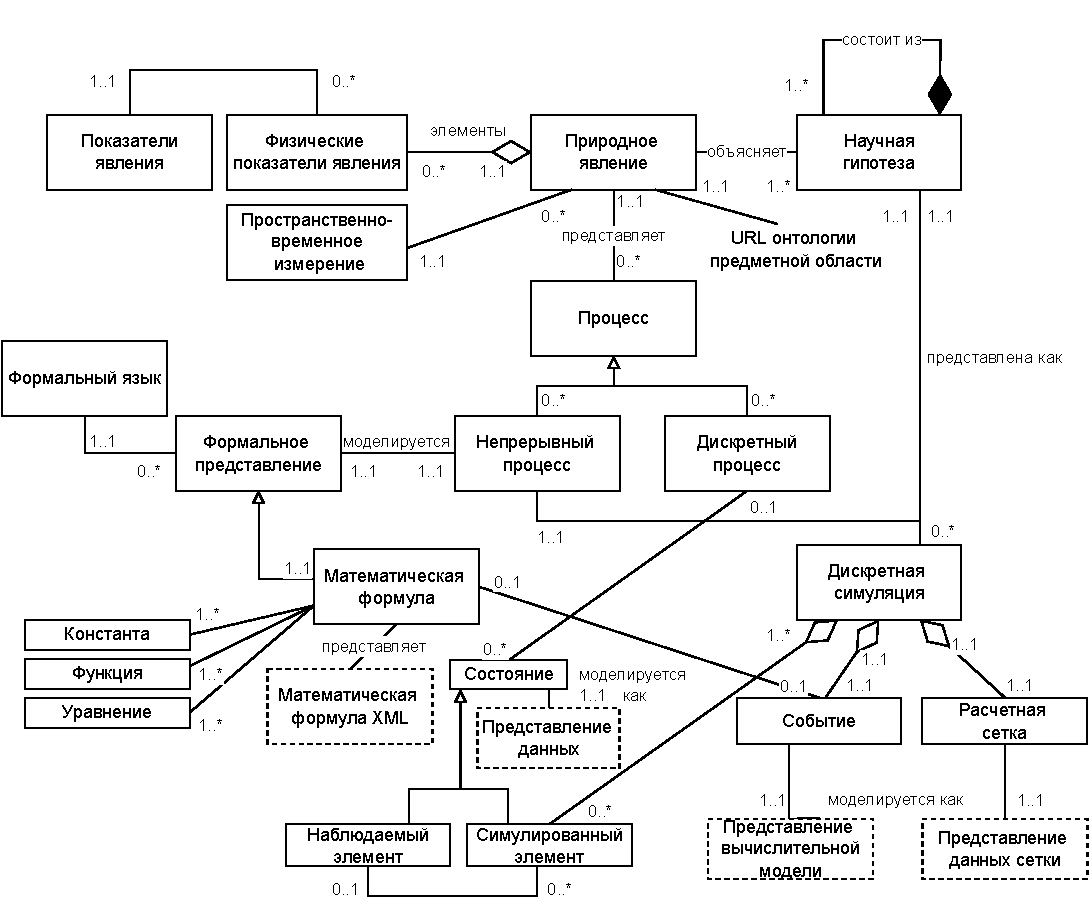
\includegraphics[width=\linewidth]{images/ScHypoConcept}
    \caption{Одна из возможных концептуализаций научной гипотезы.}\label{fig:ScHypoConcept}
\end{figure}

В работе \cite{asgharbeygi2006inductive} представлена математическая формулировка количественных моделей процессов, 
которая обеспечивает формальное кодирование научной моделей в виде системы уравнений, а также неформальное кодирование 
на языке процессов, обозначаемых этими уравнениями. Уточнение модели производится следующим образом. На входе 
необходима изначальная модель; система ограничений, представляющих допустимые изменения начальной модели на языке 
процессов; система базовых (универсальных) процессов, которые могут быть добавлены в начальную модель; наблюдения, 
которым должна соответствовать скорректированная модель. Эти данные обеспечивают эвристический подход, который 
направляет поиск на области пространства модели, которые согласуются с наблюдениями. Алгоритм генерирует множество 
уточненных моделей, которые сортируются по их удаленности от начальной модели и предлагаются вместе со своей 
среднеквадратической ошибкой на тренировочных данных. Расстояние между уточненной и начальной моделью определяется по 
количеству процессов, которые есть в одной, но нет в другой. Состоятельность такого подхода была успешно проверена в 
нескольких областях окружающей среды.

Система формирования гипотез, в основном, однообразна (монотонна) и рассматривается как не вполне подходящая для 
представления знания, в особенности при неполном знании, что часто имеет место в отношении биохимических комплексов. 
В \cite{tran2005knowledge} представлена основанная на знании структура для решения общей задачи формирования гипотез. 
Эта структура была реализована расширением основанной на знании системы <<BioSigNet-RR>>, которая поддерживает 
выработку толерантных представлений и немонотонных логических рассуждений. Главные особенности расширенной системы 
таковы, что они обеспечивают: (1) гладкую интеграцию формирования гипотез с представлением знаний и логическими 
рассуждениями; (2) использование различных ресурсов биологических данных, также как и знаний и опыта человека в целях 
разумной генерации гипотез; (3) поддержку ранжирования гипотез и дизайна экспериментов для проверки гипотез. 
Расширенная система считается прототипом интеллектуального ассистента исследователей – молекулярных биологов.

В проекте «HyBrow» (Hypothesis Space Browser – «Навигатор пространства гипотез») \cite{racunas2004hybrow} гипотезы 
в области биологии представлены как множество предложений исчисления предикатов первого порядка. Если взять сочетание н
абора аксиом, устанавливающих правила, моделирующие известные факты биологии в рамках одной и той же среды, и 
экспериментальные данные, можно обнаружить, что существующая база знаний будет либо противоречить некоторым 
предложениям гипотез, либо подтверждать их, а остальные предложения станут потенциальными открытиями. С получением 
новых экспериментальных данных и формулированием новых правил открытия становятся положительными фактами или 
опровергаются. В случае опровержений должны быть выявлены и удалены из теории, созданной на основе гипотез, те 
правила, которые себя не оправдали. При таком модельно-теоретическом подходе в вопросе подтверждения гипотез 
рассматривается удовлетворение логических импликаций, определенных в модели по отношению к интерпретации. Это может 
быть также применимо к основанным на симуляции исследованиям, где подтверждение выводится из количественного 
анализа "--- сравнения между результатами симуляции и наблюдений \cite{porto2013}. При опровержении или подтверждении 
гипотетических утверждений проект «HyBrow» берет за основу онтологию «OWL» и правила на уровне приложения. 
Проект «HyBrow» обеспечивает разработку гипотез и оценку их на непротиворечивость существующему знанию, а также 
пользуется онтологией гипотез для представления гипотез форме, приемлемой для машин: как отношения между объектами 
(агентами) и процессами \cite{soldatova2011representation}.

Инструмент «HyQue» \cite{callahan2011hyque}, новый этап развития «HyBrow», воспринимает технологии связанных данных 
и использует связанные данные «Bio2RDF», чтобы добавить к «HyBrow» возможности семантической интероперабельности. 
Гипотезы «HyBrow/HyQue» – это предметно-ориентированные утверждения, которые коррелируют с биологическими процессами 
(рассматриваемыми как события) в логике предикатов первого порядка. Гипотезы формулируются как случаи онтологии 
гипотез «HyQue» (HyQue Hypothesis Ontology) и оцениваются с помощью набора вопросов «SPARQL» в сравнении с 
биологически-ориентированными данными «OWL» и «HyBrow». Результаты вопросов оцениваются по некоторой шкале в 
зависимости от того, насколько множество событий соответствует априорным ожиданиям. Оценка по шкале показывает 
уровень поддержки гипотезы данными. Каждое событие оценивается независимо с целью квантифицировать степень поддержки, 
которое оно дает представленной гипотезе. Оценки гипотез привязываются к соответствующим гипотезам как их свойства.

Проект «OBI» (Ontology for Biomedical Investigations – Онтология биомедицинских исследований) 
\cite{brinkman2010modeling} направлен на моделирование дизайна исследования: протоколы, приборы и материалы, 
используемые в ходе экспериментов, а также генерируемые данные. Такие онтологии, как «EXPO» 
\cite{soldatova2006ontology} (см. \cref{fig:EXPO} ) и «OBI», предоставляют возможность документирования всей структуры 
научных исследований: как и с какой целью проведено исследование, какие были сделаны выводы, на какой основе и т.д. 
В результате такой однотипной процедуры по развитию онтологии в работе, заключающейся в получении минимальной 
информации по эксперименту генотипирования (MIGen), рекомендуется использование терминов, определенных в «OBI». 
Использование стандартной или совместимой онтологии для дополнения терминов будет стимулировать междисциплинарный 
доступ к данным и их дальнейшее использование. Для того чтобы сделать исследование более воспроизводимым и допускающим 
повторное использование, предусмотрен сбор возможно большого объема данных.

\begin{figure}[ht]
    \centering
    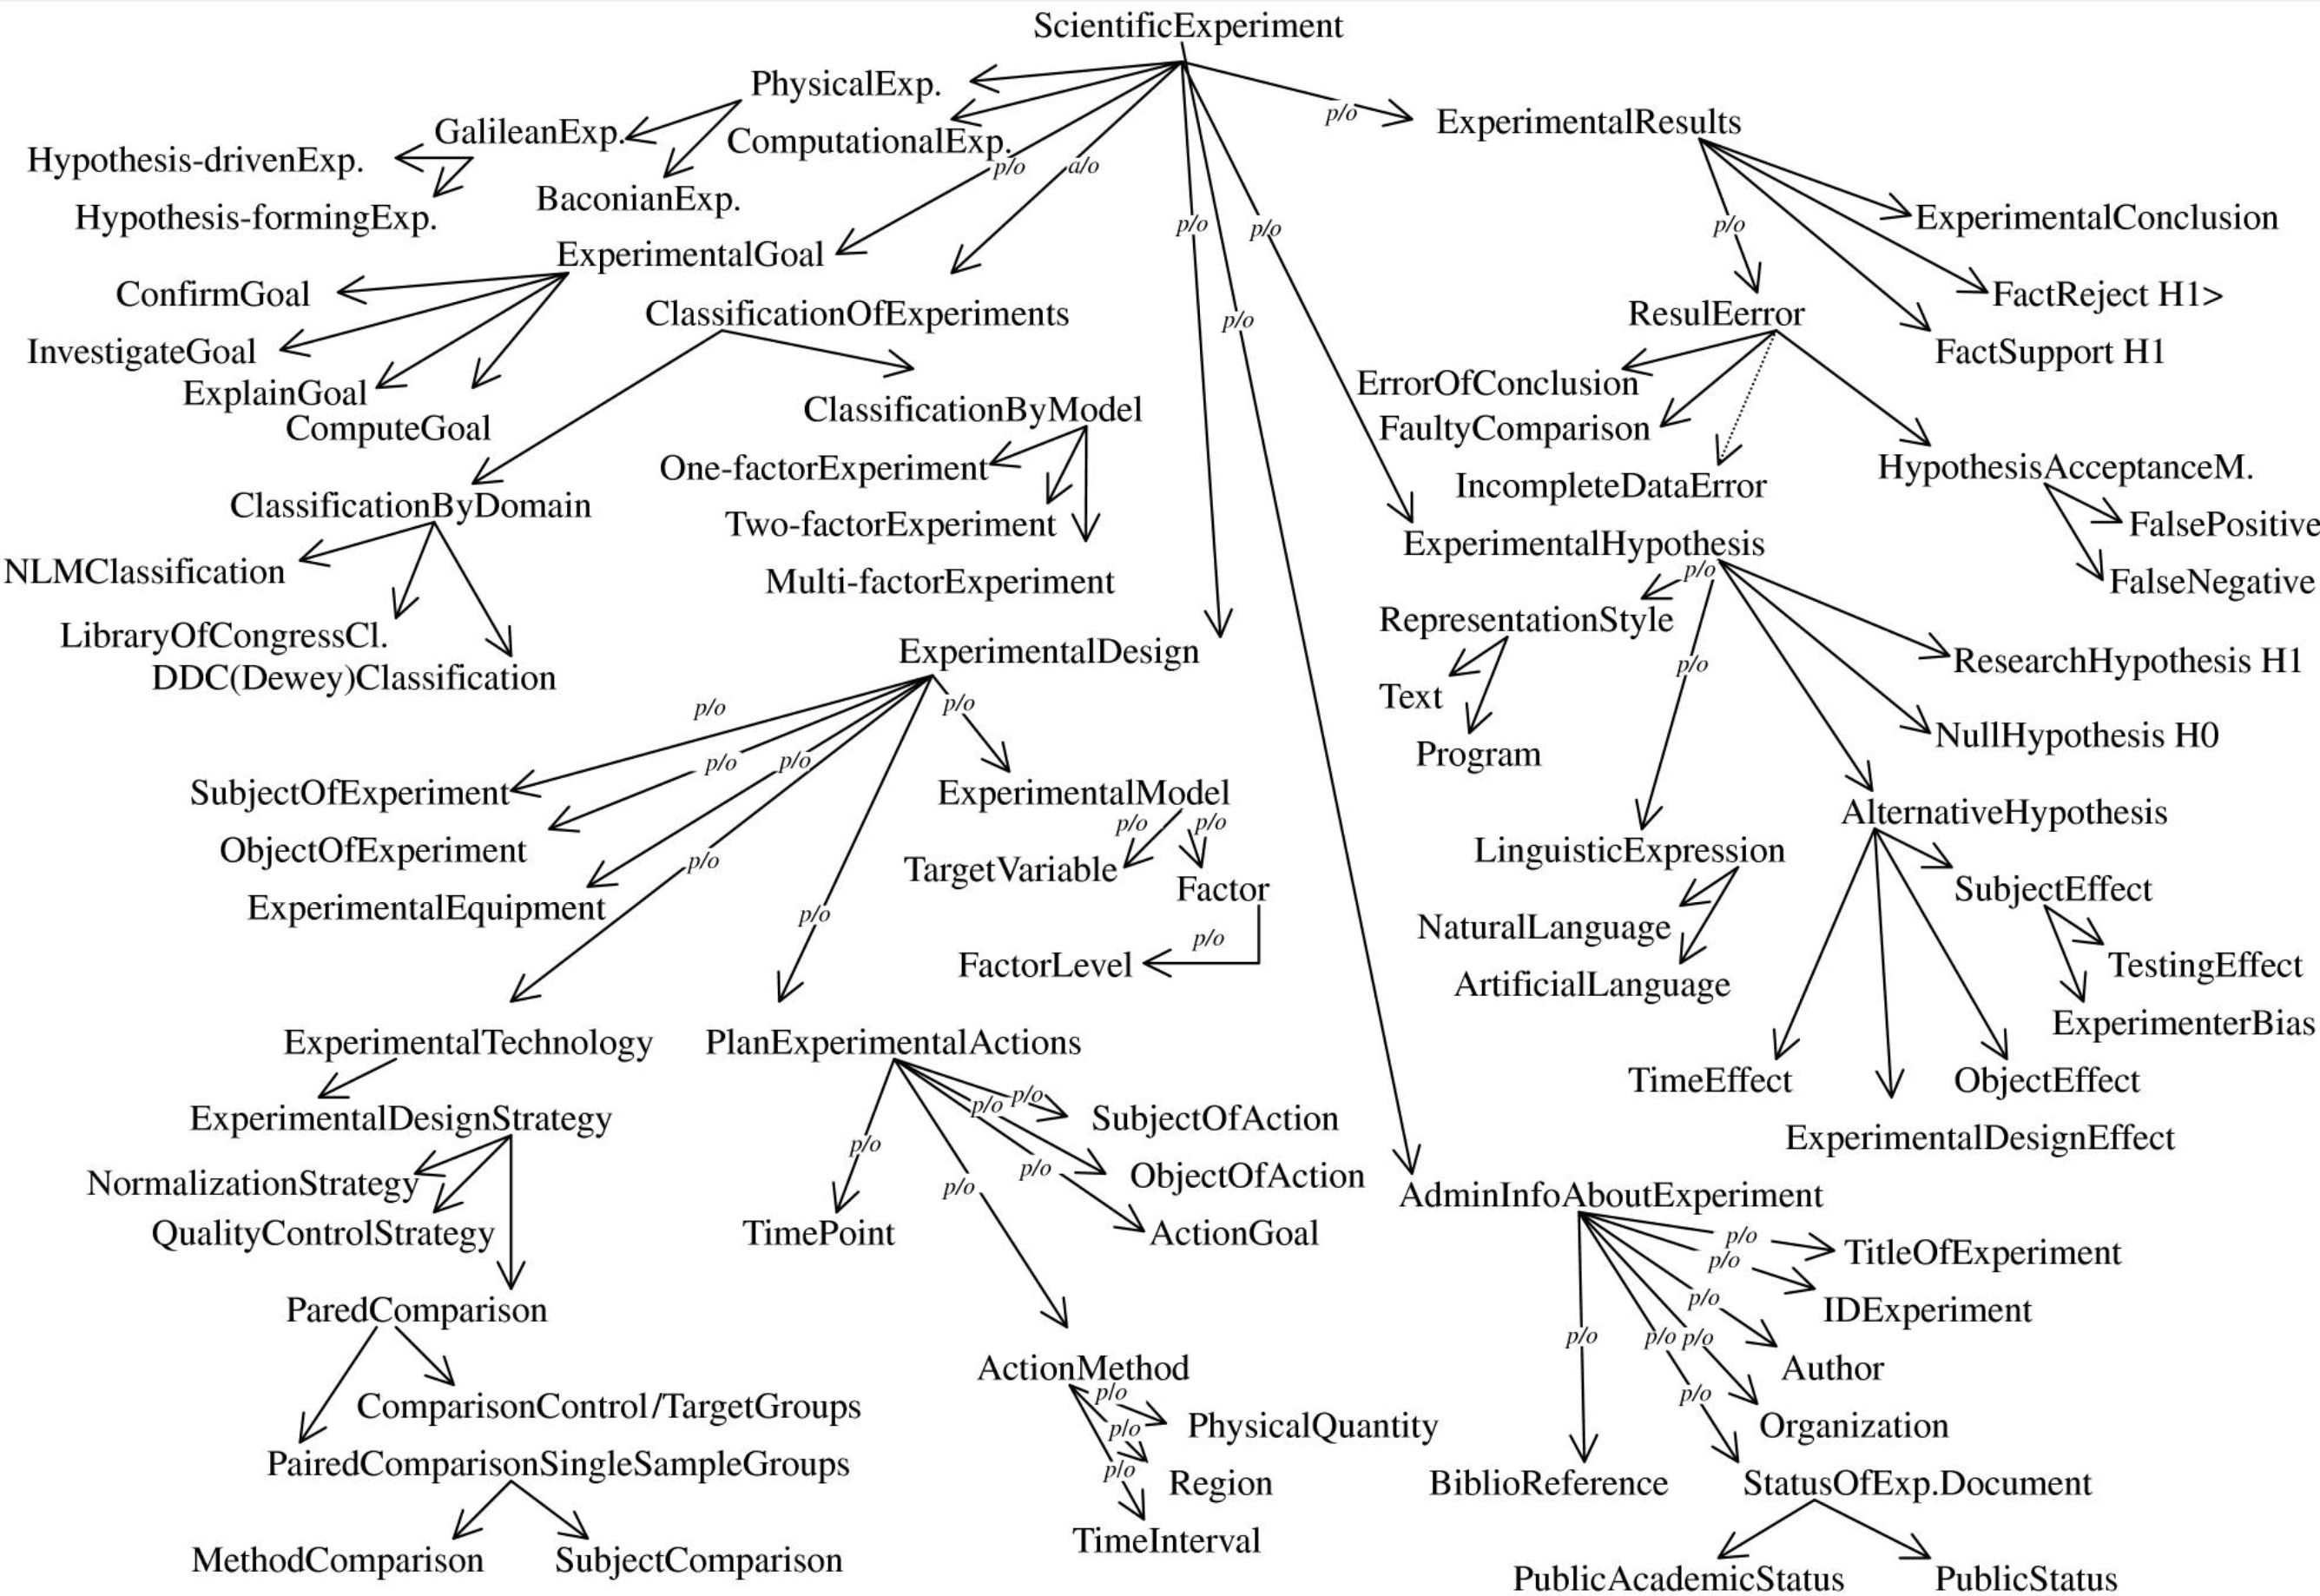
\includegraphics[width=1.0\linewidth]{images/EXPO_onto.png}
    \caption{Фрагмент онтологии научного эксперимента EXPO.}\label{fig:EXPO}
\end{figure}

Моделирование гипотез внедрено в инфраструктуры баз данных, которые развиваются в различных отраслях науки. Один из 
примеров такого рода инфраструктуры имеет наименование «SWAN» (Semantic Web Application in Neuromedicine – 
Семантическое веб-приложение «Нейромедицина») \cite{gao2006swan}. «SWAN» – это проект разработки комплексной 
инфраструктуры знаний для исследовательского сообщества по болезни Альцгеймера. Проект «SWAN» включает в своей 
онтологической модели полный жизненный цикл данных (знаний) в области биомедицинских исследований, в том числе 
организационную поддержку личных данных, генерацию гипотез, ведение экспериментов, организацию лабораторных данных 
и сотрудничество в отношении цифровых препринтов. Общая онтология указывается в «схеме» RDF. Контент проекта «SWAN» 
предназначен для охвата всех этапов процесса «открытия истины» в биомедицинских исследованиях, от формулирования 
вопросов и гипотез, получения экспериментальных данных, совместного с коллегами использования данных, вплоть до полного 
открытия и процесса публикации.

Несколько информационных категорий, которые «SWAN» создает и контролирует определены как подклассы «Утверждения». 
Они включают в себя «Публикацию», «Гипотезу», «Заявку», «Концепцию», «Манускрипт», «Массив данных» и «Аннотацию». 
«Утверждение» может опираться другое «Утверждение» или на любой объект с указанием URL. Например, ученый может 
представить «Комментарий» в отношении «Гипотезы» другого ученого или классифицировать её. Связывание с объектами 
«вне» проекта «SWAN» с помощью URL позволяет использовать информацию «SWAN» в качестве метаданных для организации, 
напр., всех публикаций PDF одного автора, или файлы Excel, в которых зафиксированы данные лаборатории, или все 
веб-сайты инструментов, имеющих отношение к нейробиологии. «Аннотация» может быть как структурированной, так и 
неструктурированной. Структурированность аннотации означает, что она привязана к «Концепции» (с помощью тега или 
термина) к «Утверждению». Неструктурированность аннотации означает привязку свободного текста. 
«Концепции» "--- это узлы вокабуляров, которые также могут быть иерархичными (таксономии).

\section{Средства поддержки экспериментов, движимых научными гипотезами}\label{sect1_3}

\subsection{Движимые гипотезами роботы. Робот-ученый Адам}\label{sect1_3_2}
«Робот-ученый» \cite{king2009automation, sparkes2010towards}, ориентированный на геномные приложения, 
является физически реализованная система, которая способна выполнять циклы научных экспериментов и делать 
открытия полностью автоматически: формирование гипотез, выбор экспериментов для проверки этих гипотез, выполнение 
экспериментов на базе робототехнической системы, анализ и интерпретация результатов, повторение цикла (система с 
обратной связью, в которой полученные результаты используются для научения и передачи полученного в результате знания 
снова в экспериментальные модели). Дедукция, индукция и абдукция "--- это виды логического рассуждения, используемого 
в научном открытии (см. \cref{sect1_2}). Полная автоматизация науки требует обучения в системе с обратной связью, где 
компьютер не только анализирует результаты, но и научается на них и отправляет полученные в результате знания назад, 
в следующий цикл процесса (\cref{fig:RobotScientistCycle}).

\begin{figure}[ht]
    \centering
    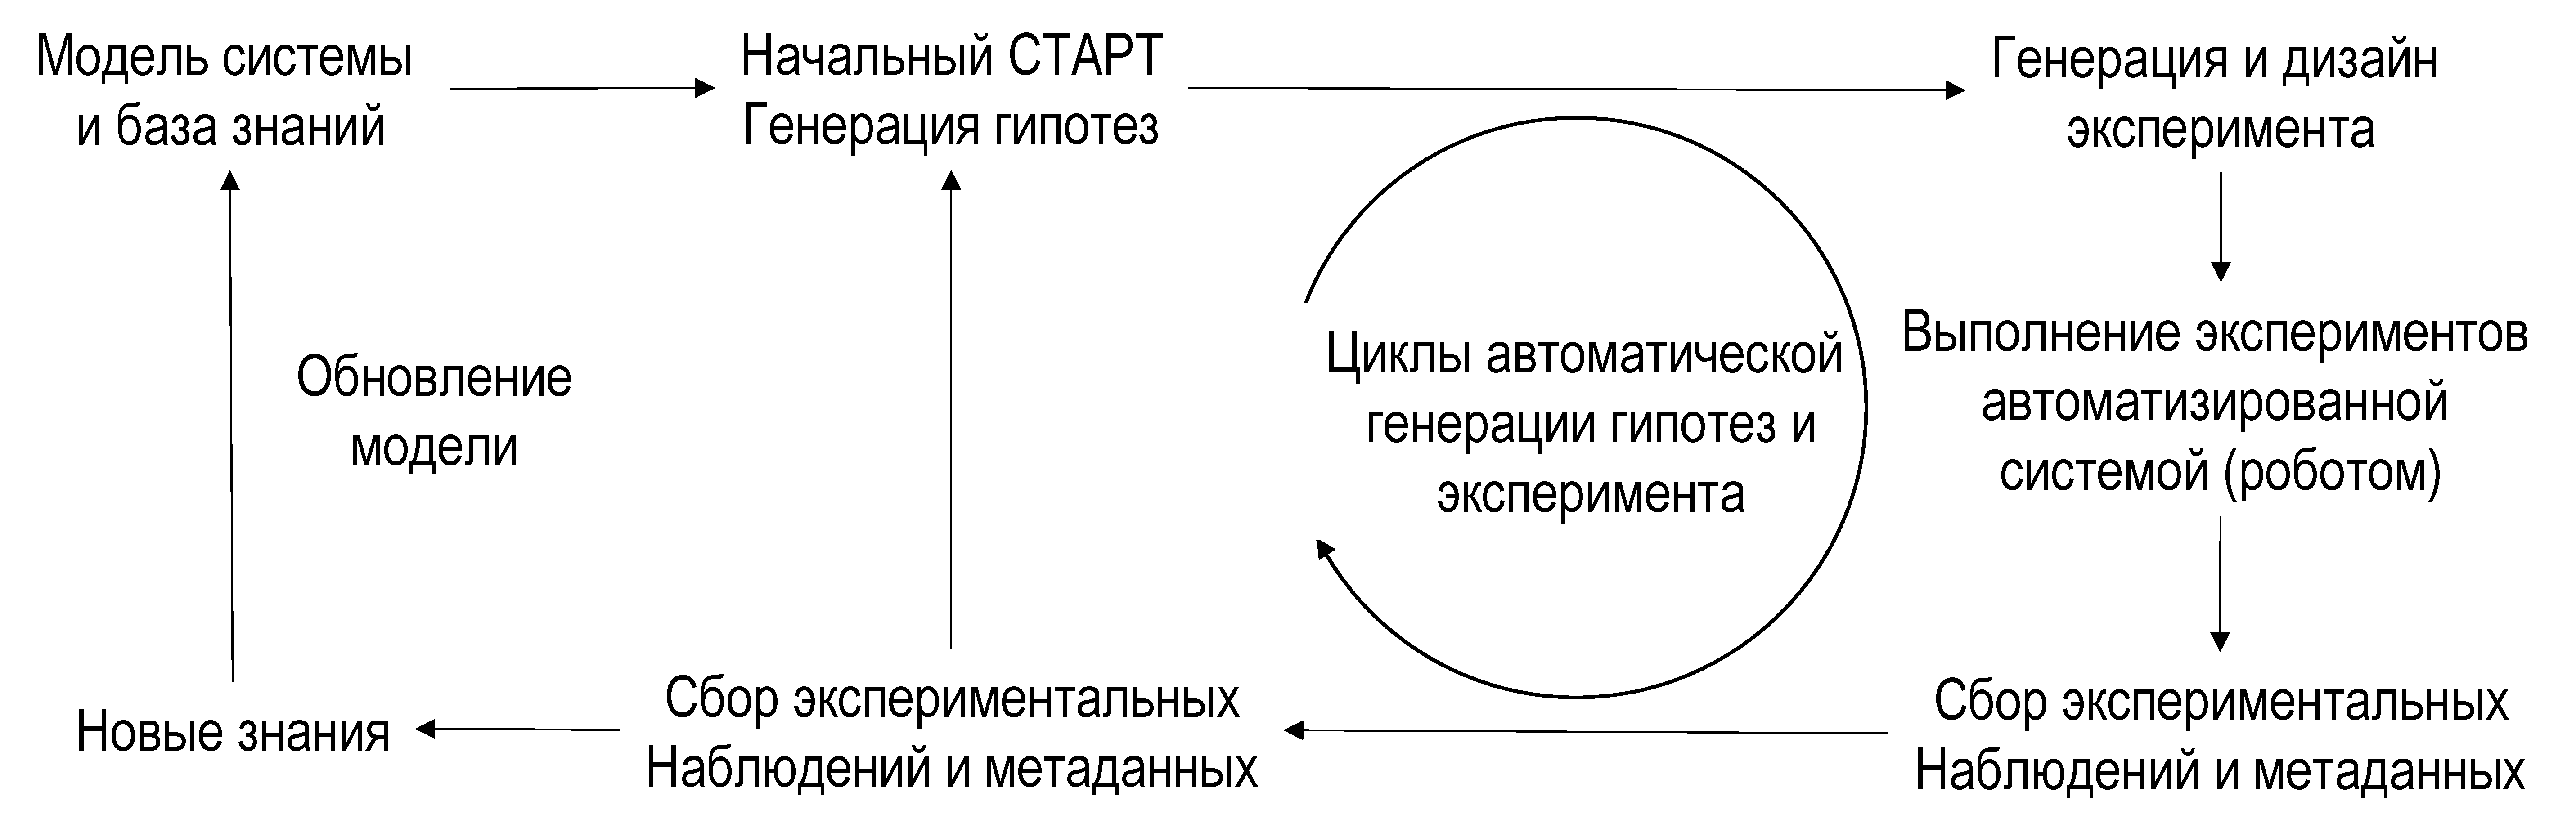
\includegraphics[width=1.0\linewidth]{images/RobotScientistCycle.pdf}
    \caption{Воплощение гипотезы.}\label{fig:RobotScientistCycle}
\end{figure}

У «Робота-ученого» автоматизированное формирование гипотез основывается на следующих ключевых компонентах:

\begin{enumerate}
    \item Рассчитываемое машиной представление знаний в данной области.
    \item Абдуктивный или индуктивный вывод новых гипотез.
    \item Алгоритм селекции гипотез.
    \item Дедукция экспериментальных следствий из гипотез.
\end{enumerate}	

«Адам», первый прототип «Робота-ученого», был разработан с целью выполнения экспериментов по выращиванию микробов 
и изучения функциональной геномики дрожжевых грибков \textit{Saccharomyces cerevisiae}, точнее говоря, для выявления 
генов, кодирующих «местно орфанные ферменты». «Адам» использует всеобъемлющую логическую модель метаболизма дрожжей в 
сочетании с биоинформационной базой данных («Kyoto Encyclopaedia of Genes and Genomes (KEGG) – Киотская энциклопедия 
генов и геномов) и стандартной биоинформационной методикой поиска гомологий («PSI-BLAST» и «FASTA») для выдвижения 
гипотез о вероятно потенциальных генах, которые могут кодировать местно орфанные ферменты. Это абдуктивный процесс 
генерации гипотез.

С целью формализации экспериментов, проводимых «Адамом» в направлении функциональной геномики, была разработана 
онтология «LABORS» («Лабораторная онтология для «Роботов-ученых»). «LABORS» является версией онтологии «EXPO» (как 
верхний слой онтологии), приспособленной для представления биологических знаний «Роботам-ученым». «LABORS» выражен 
на языке OWL DL. «LABORS» определяет различные структурные подразделения исследований, напр., испытание, собственно 
исследование, цикл исследований и воспроизведение, а также разработка стратегии, конфигурация пластины, реально 
ожидаемые результаты. Также определяются соответствующие понятия и отношения в данных функциональной геномики и 
метаданных. Как «LABORS», так и соответствующие базы данных (используемые для хранения случаев в пределах классов) 
переводятся на язык Datalog для обеспечения возможности пользования механизмом рассуждения SWI-Prolog в необходимых 
приложениях \cite{king2004functional}
.
Генерировались два уровня (вида) гипотез. Первый уровень связывает орфанный фермент, представленный своим номером 
класса ферментов (\textit{E.C.}), с геном, который (\textit{ORF}), возможно, его кодирует. Это отношение выражается 
как двухместный предикат, где первый аргумент "--- \textit{ORF}, а второй "--- номер \textit{E.C.} Пример гипотезы 
на этом уровне: \textit{encodesORFtoEC('YBR166C', '1.1.1.25')}.

Второй уровень гипотез учитывает связь между конкретным штаммом, указываемым по имени отсутствующего в нем \textit{ORF}, 
и химическим соединением, которое должно влиять на рост штамма, если в его среду добавляется питательное вещество. На 
этот уровень гипотеза выходит из первого путем логического вывода с использованием специфической модели дрожжевого 
метаболизма. Пример такой гипотезы: (влияет на рост) \textit{affects\textunderscore growth('C00108', 'YBR166C')}, где 
первый аргумент "--- химическое вещество (названия соответствуют «KEGG»), а второй аргумент "--- рассматриваемый штамм. 
Затем «Адам» проектирует экспериментальные анализы, необходимые для проверки гипотез в роботизированной лабораторной 
системе. Эксперименты основаны на двухфакторном решении, в котором проводится сравнение множественных репликатов 
анализируемых штаммов (с метаболитами и без) и диких штаммов-контролей (с метаболитами и без).

«Адам» работает в рамках гипотетико-дедуктивного метода (\cref{sect1_2_5}). «Адам» абдуктивно предполагает новые факты 
относительно функциональной биологии дрожжей, затем дедуктивно выводит экспериментальные выводы из этих фактов, 
используя свою модель метаболизма, которые затем проверяет в экспериментах. С целью выбора экспериментов «Адам» 
принимает во внимание переменные затраты на эксперименты, а также различные вероятности гипотез. «Адам» выбирает 
свои эксперименты с учетом минимизации ожидаемых затрат на исключение всех гипотез, кроме одной. В целом, это 
\textit{NP}-полная задача, и «Адам» находит решение эвристически \cite{soldatova2011representation}.

По-видимому, в настоящее время большинство гипотез в биологии генерируется компьютерами. Компьютеры всё более 
автоматизируют процесс формирования гипотез; в химии, напр., программы машинного обучения (на основе индукции) 
используются для помощи в создании лекарственных препаратов, а в биологии аннотация геномов "--- это, в сущности, 
масштабный процесс (абдуктивного) формирования гипотез. Такие компьютерно-генерируемые гипотезы, конечно, выражены в 
доступной для вычислений форме, однако вносить их в общедоступную базу данных, предоставляя для других приложений, 
пока еще не стало общей практикой \cite{soldatova2011representation}.

Подробности разработки формализации, используемой «Адамом» в исследованиях функциональной геномики, можно найти в 
работах \cite{qi2010ontology,soldatova2011representation}. Основанная на онтологии формализация, базирующаяся на 
теории графов и логическом моделировании, дает возможность безошибочно отслеживать блоки результатов, используемые 
для разных целей, сохраняя семантику всех логических категорий экспериментов, вовлеченных в полный объем исследований. 
Показано, как используются эксперименты и машинное обучение для выработки дополнительного знания в целях 
усовершенствования модели метаболизма.

В системе используются: 

\begin{enumerate}
    \item метод логического вывода новых гипотез при проведении экспериментов на основе абдуктивного логического 
            программирования для генерации достоверных гипотез, объясняющих наблюдения;
    \item метод статической оценки корректности соответствия гипотез полученным данным.
\end{enumerate}

Пользователям разрешается использовать новые метаданные для эксперимента (например, свой дизайн эксперимента). 
С использованием этого дизайна система автоматически пытается с помощью логического вывода породить новые 
гипотезы и проверить их. Дополнительно система позволяет подобрать оптимальный набор входных параметров 
итеративно на небольшом количестве начальных экспериментов, которые проводятся с различным выбором 
экспериментальных параметров.

\subsection{Гипотезы как данные в вероятностных базах данных}\label{sect1_3_3}
Еще один взгляд на кодирование и обработку гипотез представлен в работе \cite{GoncalvesP14}. Авторы работы используют 
методы вероятностных баз данных для систематического построения и обработки гипотез. Вероятностная система обработки 
баз данных «MayBMS» \cite{huang2009maybms} является ядром обработки гипотез. Эта методика (называемая 
«$\Upsilon$"---DB») дает возможность исследователям поддерживать несколько гипотез, объясняющих некоторые явления, 
и предоставляет основанный на байесовском подходе механизм оценки для ранжирования гипотез.

Построение базы данных «$\Upsilon$"---DB» включает в себя несколько этапов (см. \cref{fig:Upsilon_db_pipeline}). 
На первом этапе логические категории явлений и гипотез предлагаются как входные данные системы. Гипотеза является 
системой математических уравнений, выраженных в виде функций в формате W3C MathML; она ассоциируется с одним или не 
одним набором данных для испытания методом симулирования, где наборы данных состоят из последовательностей из $n$ 
кортежей с входными переменными уравнения и его соответствующего выхода в виде функционально зависимых \textit{FD} 
переменных (прогнозов, или предикторов). 

\begin{figure}[ht]
    \centering
    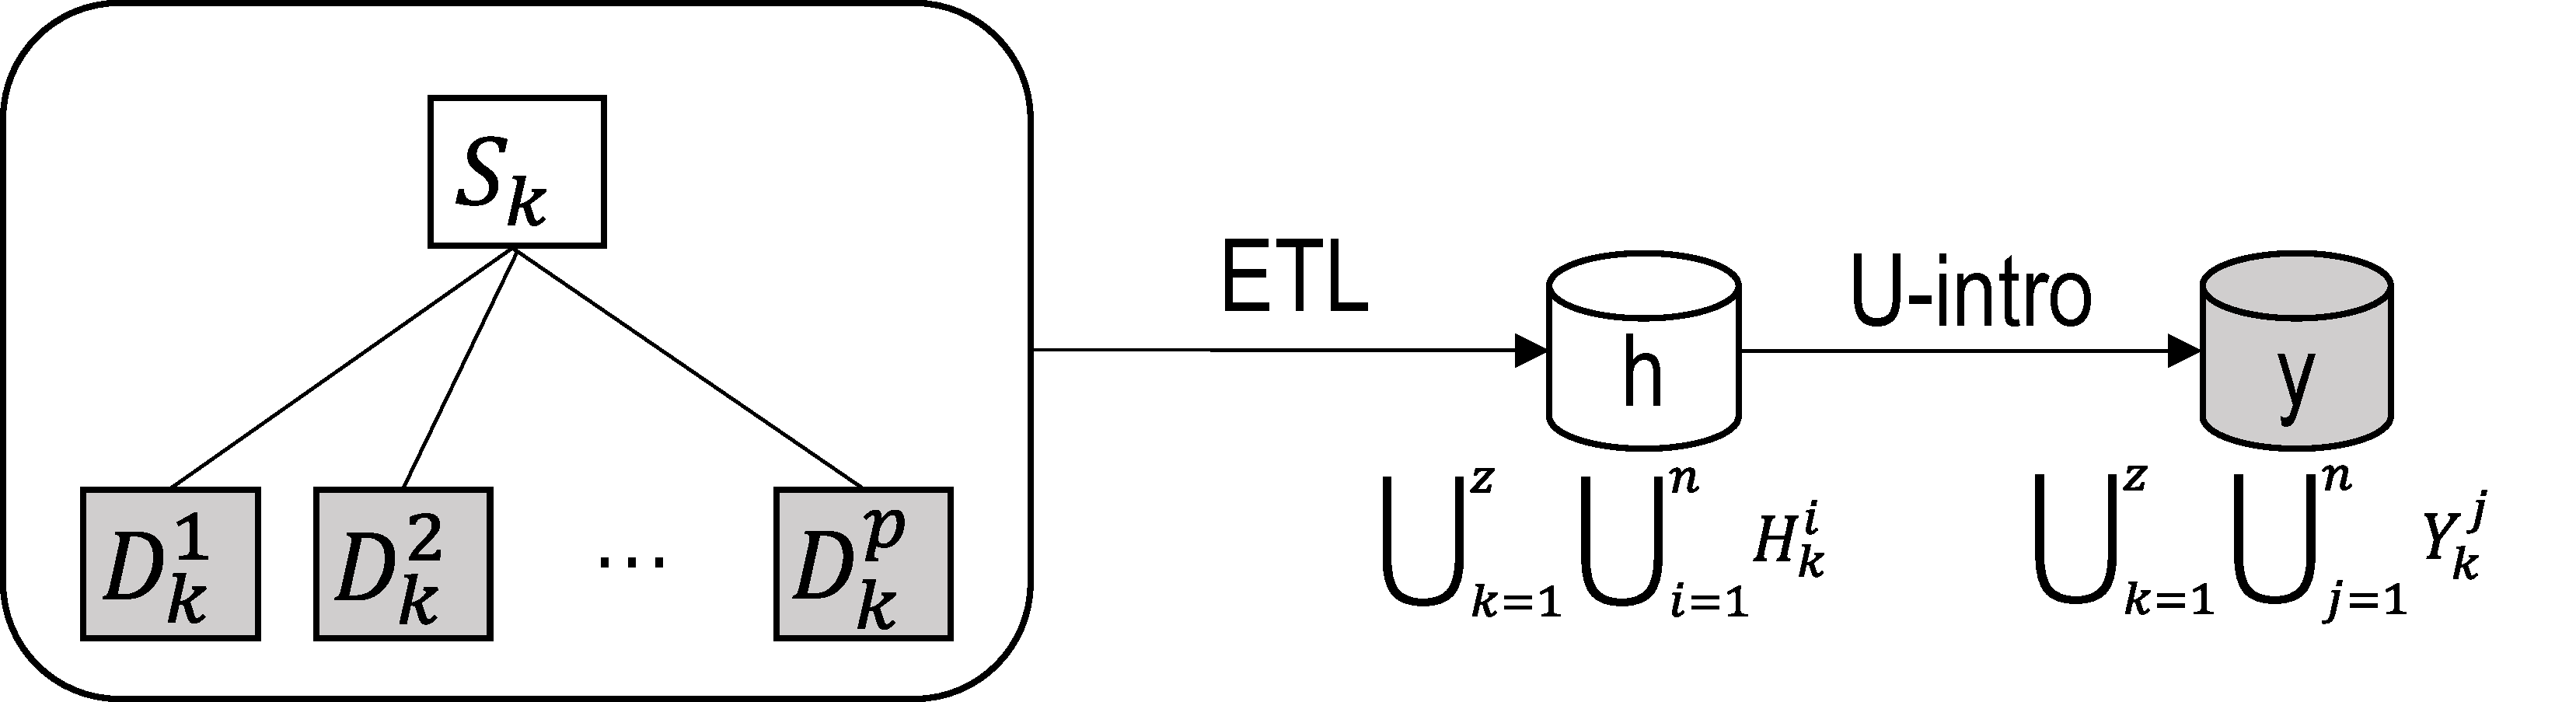
\includegraphics[width=0.7\linewidth]{images/Upsilon_db_pipeline.pdf}
    \caption{Этапы кодирования гипотез как данных в вероятностных базах данных.}\label{fig:Upsilon_db_pipeline}
\end{figure}

Явление представлено, по меньшей мере, одной эмпирической базой данных, подобной базам данных для испытания методом 
симулирования. На следующем этапе система работает с гипотезами и явлениями следующим образом: 
\begin{enumerate}
    \item исследователь должен предоставить некоторые метаданные относительно гипотез и явлений; напр., гипотезы должны 
            быть связаны с соответствующими явлениями и им должно быть приписано априорное распределение достоверности 
            (по умолчанию однородное в соответствии с принципом максимальной энтропии (\cref{sect1_2_5}));
    \item из уравнений извлекаются функциональные зависимости \textit{FD}, с тем чтобы получить схему базы данных для 
            хранения симуляций и экспериментальных данных; следует отметить, что для точного определения формулировок 
            гипотез в \textit{FD} вводятся особые атрибуты-ссылки на явления и гипотезы; 
    \item кортежи (последовательности из n членов) получаются из результатов симуляционных испытаний и наблюдательных 
            данных путем неопределенного псевдотранзитивного замыкания и логических рассуждений;
    \item наконец, формируется вероятностная база данных «$\Upsilon$"---DB». Если явление и гипотеза 
            (с эмпирическими наборами данных и симуляционными испытаниями) представлены, становится возможным 
            манипулировать ими с помощью интструментов базы данных.
\end{enumerate}

В системе при добавлении нового набора данных для всех гипотез в системе, для которых этот набор данных является 
актуальным, пересчитывается байесовская вероятность. При этом ее предыдущее значение считается априорной вероятностью, 
а по новым данным вычисляется апостериорная вероятность. При добавлении новой гипотезы в систему в виде системы 
уравнений сначала система производит ее формальное кодирование гипотез в качестве кортежей базы данныъх, а затем 
вычисляется оценка соответствия гипотез наборам данных.

В системе в качестве основных методов можно выделить:
\begin{enumerate}
    \item формальное кодирование гипотез в качестве кортежей баз данных (представление гипотез в виде систем 
            уравнений над кортежами базы данных);
    \item оценка соответствия гипотез наборам данных;
    \item построение причинно-следственных зависимостей для параметров одной гипотезы.
\end{enumerate}

Система «MayBMS» обеспечивает инструменты для оценки конкурирующих гипотез, объясняющих явление. Когда имеются 
априорные вероятности, система дает возможность сделать еще один или не один (если появляются новые данные наблюдений) 
шаг для байесовского вывода. На каждом этапе априорная вероятность обновляется, становясь в соответствии с теоремой 
Байеса апостериорной. Как результат, гипотезы, лучше объясняющие данное явление, получают более высокие вероятности, 
дающие возможность исследователям делать более достоверные заключения (см. также \cref{sect1_2_4}). 
Подход «$\Upsilon$"---DB» обеспечивает перспективный путь анализа гипотез в области масштабных ИИИД, являясь 
непостоянной прогнозирующей (предикторной) базой данных, учитывающей эмпирические данные.


\subsection{Система поддержки научных исследований <<Гефест>>}\label{sect1_3_4}
В основе системы <<Гефест>> (Hephaestus) \cite{Duggan2015} лежит работа с виртуальными экспериментами над данными. 
Система помогает исследователю искать корреляционные зависимости между большим числом переменных, предоставляет 
возможность сформировать гипотезы по наиболее перспективным связям, а затем с помощью тщательного тестирования перейти 
к причинно-следственной зависимости. 

Система позволяет исполненять виртуальный эксперимент над существующими базами данных, которые могут выполнять 
некоторую аналитику локально. Она ориентирована на работу с очищенными и размеченными данными. Система состоит из 
следующих модулей:
\begin{itemize}
    \item Компонент для работы с наборами данных. Авторы стремятся создать некую поисковую систему, которая принимает 
            на вход строку, описывающую параметры гипотезы, возвращает ранжированный список потенциальных 
            причинно-следственных зависимостей.
    \item Компонент тестирования гипотез. Является основным компонентом системы. Движок составляет запрос для оценки 
            каждого возможного взаимодействия, разбивает образцы на контрольные блоки и высчитывает заданную метрику 
            точности для каждого из них. После расчета статистики для блока, движок объединяет результаты, получая 
            взвешенную оценку гипотезы.
    \item Компонент ранжирования результатов. Гипотезы объединяются и сортируются по некоторой вероятностной оценке.
\end{itemize}

Центральным блоком системы является SQL-подобный декларативный язык для описания виртуального эксперимента, 
с помощью которого возможно проектировать дизайн эксперимента, специфицировать основные гипотезы и их параметры, 
тестировать их, исполнять выбранные эксперименты и публиковать исследования. Так как применение только статистических 
методов и машинного обучения может приводить к ошибочным результатам в поиске причинно-следственных связей, то системы 
ориентирована на симбиоз между человеком и машиной. Используя корреляционные связи, которые были проверены экспертами 
в предметной области, <<Гефест>> собирает вероятностно причинные графы для спецификации семантики предметной области. 
Причинный граф поддерживает большое количество связей, обнаруженных в процессе выполнения виртуального эксперимента, 
а также позволяет исследовать последовательность выявления вероятностных причин и аномалий. Система позволяет отсекать 
некоторые неперспективные вычислительные маршруты c точки зрения конечных метрик, 
минимизируя общее количество вычислений.

Основными методами для манипулирования гипотезами и виртуальными экспериментами являются:
\begin{enumerate}
    \item метод автоматического порождения гипотез из данных "--- символьная регрессия при подборе аппроксимирующей 
            формулы для выбранного подмножества переменных на наборе данных;
    \item метод интервенций при исполнении виртуального эксперимента - установление существующих и возможной 
            генерации новых гипотез, которые значимо влияют на выбранную экспертом гипотезу;
    \item метод корректного разбиения данных наблюдений при проверке статистических гипотез для обеспечения 
            несмещенных оценок при дальнейшем тестировании гипотез;
    \item метод ранжирования нескольких конкурирующих гипотез, наиболее соответствующих наблюдениям, 
            по выбранной метрике (например, достигаемому уровню значимости) или нескольким метрикам;
    \item метод построения графа причинно-следственных и вероятностных зависимостей для оценки соответствия 
            полученных зависимостей общепринятым в области, а также для потенциального исследования значимых 
            корреляций и их последующего преобразования в причинно-следственные зависимости.
\end{enumerate}

При добавлении нового набора данных или объединении нескольких разрозненных наборов данных применяется следующая 
процедура. Система вычисляет выбранные метрики точности каждого набора данных независимо и вычисляет их взвешенную 
сумму для последующей оценки гипотезы. Разработчик эксперимента сам выбирает весовую функцию. При этом рекомендуется 
учитывать такие факторы, как размер или дисперсия выборки каждого набора данных. Система в автоматическом режиме не 
выполняет слияние всех наборов данных в один большой набор. Так как разные наборы данных могут содержать не все 
переменные, то система с использованием линейной регрессии может построить зависимость отсутствующих переменных по 
другим наборам данных и восстановить их при необходимости, если это требуется для корректной оценки гипотезы.

\subsection{Не гипотезо-ориентированные системы}\label{sect1_3_5}

Система FCCE \cite{schales2015fcce} предназначена для поиска корреляций в неоднородных наборах данных, охватывающих 
большие диапазоны времени. Ключевым компонентом модели данных является концепция функций. Функции определяют отношение 
между ключом и некоторым значением, каждый элемент которого может содержать несколько функций. FCCE представляет 
упрощенную модель реляционных данных для пользователя, где каждая таблица хранит один тип характеристики. Каждая 
строка идентифицируется по ключу и может содержать несколько функций. В системе FCCE ключевым методом является 
построение попарных корреляционных зависимостей для всех переменных множества разрозненных наборов данных. Для метода 
существует распределенная реализация, позволяющая искать значимые корреляции между разнообразным набором данных разных 
типов, при этом используются различные временные окна. Данная система рассматривалась на примере двух задач из области 
безопасности: обнаружения доменных имен потенциальных сетей зараженных рабочих станций и пост-инцидентное расследование 
проникновения. Для минимизации задержек обработки данных решено было отказаться от использования традиционных 
реляционных баз данных для хранения информации и перейти на NoSQL. Ключевым компонентом модели данных является 
концепция признаков. Признаки определяют связь между парой ключ-значение, каждый элемент из которых может содержать 
несколько атрибутов. FCCE представляет упрощенную реляционную модель данных для пользователя, где каждая таблица хранит 
один тип признаков. Каждая строка идентифицируема ключом и может содержать несколько атрибутов. FCCE обеспечивает 
API для хранения, получения и вычисления корреляции над признаками. Разработчики предлагают оригинальный подход 
интеграции модуля оценки критерия корреляции в движок исполнения запросов над хранилищем, позволяющий ускорить время 
ответа на запрос и снизить накладные расходы на вычисление и вводвывод. FCCE использует два отличительных механизма 
для поддержки эффективности операций нахождения корреляций между признаками: канал запросов и модификатор запросов. 
Канал "--- механизм, позволяющий передавать признаки, извлеченные из одного запроса в другой запрос в качестве входных 
данных, т.е. последовательно можно объединять несколько GET функций, тем самым создавай пересечения нескольких 
признаков. Модификатор – над GET запросом предполагает использование широкого набора опций для более тонкого контроля 
его поведения.

%TODO недостатки SDI
Платформа SDI \cite{demchenko2013addressing}  используется для поддержки научных экспериментов. Система может 
интегрировать открытые данные, повторно использовать данные наблюдений и данные моделирования при эволюции виртуальных 
экспериментов. SDI требует поддержки происхождения, классификации, индексации экспериментов и данных, полного цикла 
получения данных, их обработки и очистки, создания экспериментов для проверки гипотез над большими коллекциями данных, 
агрегирования результатов в течение продолжительных периодов времени. Платформа также позволяет интегрировать открытые 
данные, повторно использовать данные наблюдений и данные моделирования при эволюции виртуальных экспериментов. 
Вместе с тем, SDI не позволяет непосредственно работать с гипотезами, не устанавляваются зависимости между гипотезами 
в одном эксперименте.

MLCask \cite{Luo2021} "--- это git-подобная ветвящаяся система, предназначенная для обработки нелинейных моделей 
машинного обучения и конвейеров данных. Это позволяет совместно разрабатывать конвейер и повторно использовать 
промежуточные результаты вычислений для сокращения продолжительности операции слияния на основе выбранной метрики. 
Система не имеет прямого отношения к понятию гипотезы и каким-либо взаимозависимостям между ними. Кроме того, проверка 
гипотез не является частью системы.

MLflow \cite{Zaharia2018} и Dagster \cite{Dagster2022} "--- это программные пакеты, которые предоставляют API для 
выполнения конвейеров машинного обучения. Позволяет хранить кэшированные результаты выполнения функции. Эти системы 
позволяют отслеживать выполнение на предмет происхождения, повторного использования конфигурации, а также упаковки и 
развертывания модели, хранения показателей и ранжирования. Эти системы не отслеживают никаких зависимостей между 
экспериментами, поэтому выбор конкурирующих или производных моделей осуществляется экспертом.

MLDev \cite{Khritankov2022} "--- это программный инструмент, ориентированный на воспроизводимость эксперимента, 
который имеет отдельную спецификацию, которая обеспечивает порядок вычисления нескольких гипотез. MLDev использует 
вычислительно-ориентированную структуру леса для определения порядка выполнения и вызовов функций. Система не 
анализирует зависимости каких-либо гипотез друг от друга.

\subsection{Требования к системе/платформе поддержки научных исследований}\label{sect1_3_7}

Сравнение систем поддержки научных исследований представлено в \cref{tbl:comparison}. Анализ показывает, 
что существующие системы не охватывают несколько важных вопросов, в том числе взаимодействие между гипотезами в 
одном эксперименте, отслеживание эволюции эксперимента, восприятие автоматически полученных гипотез и формул экспертами.

\begin{table} [ht]%
	\caption{Сравнение систем поддержки научных исследований}%
	\label{tbl:comparison}% label всегда желательно идти после caption
    \setlength\extrarowheight{0pt} %вот этим управляем расстоянием между рядами, \arraystretch даёт неудачный результат
    \setlength{\tymin}{2.3cm}% минимальная ширина столбца
	\begin{tabulary}{\textwidth}{@{}>{\zz}L >{\zz}L >{\zz}L >{\zz}L@{}}% Вертикальные полосы не используются 
        %принципиально, как и лишние горизонтальные (допускается по ГОСТ 2.105 пункт 4.4.5) % @{} п
        %озволяет прижиматься к краям
        \toprule     %%% верхняя линейка
    	Название &
    	Ключевые элементы &
    	Слабые стороны &
    	Сильные стороны	\\
        \midrule %%% тонкий разделитель. Отделяет названия столбцов. Обязателен по ГОСТ 2.105 пункт 4.4.5 
        <<Робот-ученый>> &
        Использование онтологий, абдуктивного и логического вывода. Физически построенная лаборатория.  &
        Невозможность работать с формулами. Громоздкая онтология эксперимента/ 
        Ориентированность применения --- биоинформатика, ведет к своей интерпретации 
        определения виртуального эксперимента. &
        Возможность проверять тысячи гипотез автоматизированно в реальности. 
        Использования логический вывода для порождения новых гипотез.
        
        \\
        \midrule %%% тонкий разделитель. Отделяет названия столбцов. Обязателен по ГОСТ 2.105 пункт 4.4.5 
        <<Гефест>> &
        Собственный SQL-подобный язык запросов для описания эксперимента. Основной элемент --- виртуальный эксперимент. 
        Построение вероятностно-причинных графов. Мета-система --- работает над существующими базами данных. &
        Интеграция данных не предоставляется из коробки. Плохое описание модуля поиска корреляций. 
        Ориентированность применения --- здравоохранение, ведет к своей 
        интерпретации определения виртуального эксперимента. &
        Тестирование и ранжирование гипотез на основе частотной статистики.
        Граф знаний может визуализировать результаты и помогать интегрировать новые гипотезы. 
        Работает с наборами гипотез.
        \\
        % \midrule
        % FCCE &
        % Использование NoSQL БД. Основной элемент – концепция функций. API поддержки для хранения, 
        % извлечения, оценки корреляции по признакам.
        % Комплексная многоуровневая система агрегации данных. 
        % &
        % Не описан модуль корреляций. Ориентированность применения – анализ поведения сети. 
        % Не оперирует математическими формулами. 
        % &
        % Сосредоточение на минимизации задержек.Поддержка доступа к сырым данным. Быстрый модуль поиска корреляций. 
        % Программно реализован.
        % \\
        \midrule
        $\Upsilon$-DB &
        Основной элемент – поддержка научных исследований. Вероятностная БД.Работа с отдельными гипотезами.
        Байесский подход. Гипотезы в формате MathML. &
        Взаимосвязь гипотез выходит за рамки системы. Проблемы с масштабируемостью. &
        СУБД на базе SQL. Автоматически пересчитывает вероятность после получения новых данных или гипотезы. 
        Работает с формулами.
        \\
        \midrule
        & &  & \scriptsize (продолжение следует)
        \\
        \bottomrule %%% нижняя линейка
	\end{tabulary}%
\end{table}

\begin{table} [ht]%
	\caption*{}%
	%\label{tbl:comparison}% label всегда желательно идти после caption
    \setlength\extrarowheight{0pt} %вот этим управляем расстоянием между рядами, \arraystretch даёт неудачный результат
    \setlength{\tymin}{2.3cm}% минимальная ширина столбца
	\begin{tabulary}{\textwidth}{@{}>{\zz}L >{\zz}L >{\zz}L >{\zz}L@{}}% Вертикальные полосы не используются 
        % принципиально, как и лишние горизонтальные (допускается по ГОСТ 2.105 пункт 4.4.5) % @{} 
        % позволяет прижиматься к краям
        \toprule     %%% верхняя линейка
        \scriptsize (продолжение) & & &
        \\
        \midrule
    	Название &
    	Ключевые элементы &
    	Слабые стороны &
    	Сильные стороны	\\
        \midrule %%% тонкий разделитель. Отделяет названия столбцов. Обязателен по ГОСТ 2.105 пункт 4.4.5 
        
        SDI &
        Система поддержки научных экспериментов. Работа на всех уровнях, включаю интеграцию данных и исполнение 
        эксперимента. &
        Не позволяет непосредственно работать с гипотезами, не устанавляваются зависимости между гипотезами в 
        одном эксперименте.   &
        Повторное использование данных моделирования, тестирование гипотез в экспериментах, интеграция данных, 
        фиксирование эволюции эксперимента.
        \\
        \midrule
        FCCE &
        Использование NoSQL БД. Основной элемент – концепция функций. API поддержки для хранения, извлечения, 
        оценки корреляции по признакам.
        Комплексная многоуровневая система агрегации данных. 
        &
        Не описан модуль корреляций. Ориентированность применения – анализ поведения сети. 
        Не оперирует математическими формулами. 
        &
        Сосредоточение на минимизации задержек.Поддержка доступа к сырым данным. Быстрый модуль поиска корреляций. 
        Программно реализован.
        \\
        \midrule
        MLCask &
        git-подобная ветвящаяся система. Конвейер для выполнения нелинейных моделей. &
        Не использует понятия гипотезы и зависимостей между ними. Проверка гипотез не является частью системы. &
        Воспроизводимость результатов, хранение и повторное использование промежуточных результатов.
        \\
        \midrule
        & &  & \scriptsize (продолжение следует)
        \\
        \bottomrule %%% нижняя линейка
	\end{tabulary}%
\end{table}

\begin{table} [ht]%
	\caption*{}%
	%\label{tbl:comparison}% label всегда желательно идти после caption
    \setlength\extrarowheight{0pt} %вот этим управляем расстоянием между рядами, \arraystretch даёт неудачный результат
    \setlength{\tymin}{2.3cm}% минимальная ширина столбца
	\begin{tabulary}{\textwidth}{@{}>{\zz}L >{\zz}L >{\zz}L >{\zz}L@{}}% Вертикальные полосы не используются 
        % принципиально, как и лишние горизонтальные (допускается по ГОСТ 2.105 пункт 4.4.5) % @{} 
        % позволяет прижиматься к краям
        \toprule     %%% верхняя линейка
         \scriptsize (продолжение) & & & 
        \\
        \midrule
    	Название &
    	Ключевые элементы &
    	Слабые стороны &
    	Сильные стороны	\\
        \midrule %%% тонкий разделитель. Отделяет названия столбцов. Обязателен по ГОСТ 2.105 пункт 4.4.5 

        MLFLow/ Dagster &
        Программные пакеты, которые предоставляют API для выполнения конвейеров машинного обучения 
        &
        Не отслеживают никаких зависимостей между экспериментами, поэтому выбор конкурирующих или производных моделей 
        осуществляется вручную. Не используют понятине гипотез.
        &
        Позволяет хранить промежуточные вычисления. Эти системы позволяют отслеживать происхождение, повторного 
        использовать конфигурации, а также упаковывать и развертывать модели, фиксируют метрики.
        \\
        \midrule
        MLDev &
        Поддержка развития моделей машинного обучения. Ориентированный на воспроизводимость эксперимента. &
        Взаимосвязь гипотез выходит за рамки системы. Отсутствие формульного подхода к гипотезам &
        Сохранение эколюции эксперимента, спецификация отдельных гипотез и эксперимента для воспроизводимости.
        \\
        \bottomrule %%% нижняя линейка
	\end{tabulary}%
\end{table}


В результате анализа сформулированы общие требования к системе для управления виртуальными экспериментами:
\begin{enumerate}
    \item Отслеживание эволюции моделей, гипотез и экспериментов, добавление новых источников данных. 
            Должны быть определены операции управления виртуальными экспериментами и их составляющими 
            (гипотезы, модели, их конфигурации).
    \item Обеспечение явной спецификации зависимостей между гипотезами (например, конкурирующие гипотезы, одна гипотеза 
            выведена из другой), автоматического извлечения зависимостей между гипотезами. Учет корреляции между 
            параметрами нескольких гипотез и автоматическое извлечение корреляций. Использование полученных 
            зависимостей и корреляций при принятии решения, от каких конфигураций экспериментов следует заранее 
            отказаться. Так, например, некоторые сочетания гипотез и/или их параметров могут приводить к противоречию с 
            базовыми физическими законами (также определенными как гипотезы в виртуальном эксперименте). Необходима 
            также предварительная идентификация и фильтрация виртуальных эксперименты с предсказуемо плохо 
            соответствующим наблюдениям результатом.
    \item Обеспечение ранжирования экспериментов и конкурирующих гипотез по соответствию наблюдаемым данным на 
            одном или нескольких наборах данных. Вычисление метрики соответствия, используемой для принятия решения об 
            отказе от эксперимента, плохо соответствующем наблюдениям, на новом наборе данных (при этом происходит 
            ограничение количества возможных экспериментов).
    \item Предоставление структур для хранения результатов предыдущих экспериментов, и обеспечение запросов к ним. 
            План проведения экспериментов должен быть сформирован таким образом, чтобы сохраненные результаты по 
            возможности использовались, и никаких повторных вычислений не производилось.
    \item Повторное использование программ и данных компьютерами, а также воспроизводимость экспериментов 
            \cite{Gundersen2018} требует использования формальных спецификаций предметных областей данных, а также 
            поддержки автоматического логического вывода. Разработка формальных концептуальных спецификаций в научных 
            сообществах стимулируется необходимостью достижения семантической интероперабельности между коллекциями 
            данных и компонентами. 
    \item Система должна быть модульной и функционально расширяемой, а также должна поддерживать связность с другими 
            компонентами глобальной системы, в рамках которой она реализуется.
\end{enumerate}

\section{Выводы по главе}\label{sect1_4}

\FloatBarrier
           % Глава 1
\chapter{Метод управления виртуальным экспериментом в исследованиях с интенсивным использованием данных} \label{chapt2}
\newtheorem{mydef}{Definition}

\section{Концептуализация экспериментов}\label{sect1_2_6}

ИИИД становится во все возрастающей степени начинают зависеть от вычислительных ресурсов, которые оказывают помощь в 
комплексных исследованиях. Исключительно важным становится предоставление ученым инструментов, необходимых для работы 
с разнообразными данными, получаемыми в ходе подобных исследований. Изучаются конкретные концептуально моделирующие 
средства \cite{porto2013}, дающие возможность ученым представлять научные гипотезы, модели и связанные с ними расчетные 
или симулирующие интерпретации, которые можно сравнить с наблюдениями явлений \cref{fig:hypothesis_real}. Модель 
позволяет ученым фиксировать существующее знание относительно наблюдаемого и исследуемого явления, включая его 
формальную математическую интерпретацию, если она существует. Необходимо также поддерживать эволюцию модели и её 
коллективное использование с точки зрения математики или вычислений (напр., в форме потоков автоматизированного 
управления научными исследованиями). Декларативное представление научной модели дает возможность ученым сосредоточиться 
на исследовании научных вопросов. Для преодоления разрыва между онтологическим описанием изучаемого явления и его 
симуляциями могут быть также использованы гипотезы. Концептуальные воззрения относительно сущностей области науки 
позволяют осуществлять поиск определений, поддерживающих распространение научных моделей между разными 
научными группами. 

В \cite{Goncalves2013} рассматривается создание гипотезы как проработка связанных данных. Семантический взгляд на 
научные гипотезы демонстрирует их существование отдельно от формулировок конкретных утверждений в некоторой 
математической структуре. Математическое уравнение считается недостаточным для идентификации гипотезы; во-первых, 
потому, что она должна иметь физическую интерпретацию, а во-вторых, потому что возможно несколько способов 
формулирования одной и той же гипотезы. Связь с математическим выражением, тем не менее, дает гипотетической 
концепции более высокую семантическую точность. В дополнение к этому, еще одна формулировка явного описания 
объясняемого явления (с ударением на его «физическую интерпретацию») может сделать вкладываемый смысл очевидным. 
Работая с такой гипотезой как с концептуальной сущностью, ученые приводят к возможности изменить формулировку 
утверждения или даже предложить семантическое отображение на другое воплощение гипотезы, если кто-либо еще 
переформулирует её.

В работе \cite{porto2013} концептуализируются следующие элементы, связанные с наукой, движимой гипотезами: 
наблюдаемое явление, интерпретирующее это явление модель, а также метаданные, определяющие соответствующие вычисления 
с симулирующим определением (для симуляции предлагается основанный на логике декларативный язык). Особое внимание в 
этой работе уделяется определению гипотез. Объяснение, которое дает научная гипотеза, выражает отношение между 
каузальными явлениями и, а именно то, что симулируемое явление является следствием каузальных явлений или возникло 
при наличии условий, обусловленных каузальными явлениями. Выполняя симуляции, определяемые антецедентами каузальных 
отношений, ученый направляет усилия на анализ гипотезы, стоящей за изучаемым явлением.

Итак, научная гипотеза становится элементом научной модели, которая может заместить явление. Когда производятся 
вычисления симуляции, основанной на научной гипотезе, т.е. в соответствии с причинно-следственной связью, которую 
она устанавливает, результаты на выходе можно сравнивать с наблюдениями явления, с тем чтобы оценить качество гипотезы. 
Такая интерпретация обеспечивает преодоление разрыва между качественным описанием пространства явления (научные 
гипотезы могут быть использованы в качественных (т.~е., онтологических суждениях)) и соответствующей количественной 
оценкой, получаемой посредством симуляции. В соответствии с подходом \cite{porto2013} комплексные научные модели могут 
быть выражены сочетанием вычислительных моделей подобно тому, как это рассматривается в отношении баз данных.

Показанный на \cref{fig:ScHypoConcept} пример разнообразия компонентов научной модели гипотез был взят из приложений 
<<Нейромедицина>> \cite{porto2013, porto2012scientific} и по сердечно-сосудистой системе человека в 
<<Вычислительной гемодинамике>> \cite{Goncalves2013, Porto2011}. Формализация научной гипотезы была обеспечена 
математической моделью, системой дифференциальных уравнений для непрерывных процессов, квантификацией варьирования 
физических величин в непрерывном пространстве-времени, а также решателем математических задач <<HEMOLAB>> для 
дискретных процессов. Математические уравнения были представлены на языке MathML, дающем моделям возможность 
повторного использования. 

\begin{figure}[ht]
    \centering
    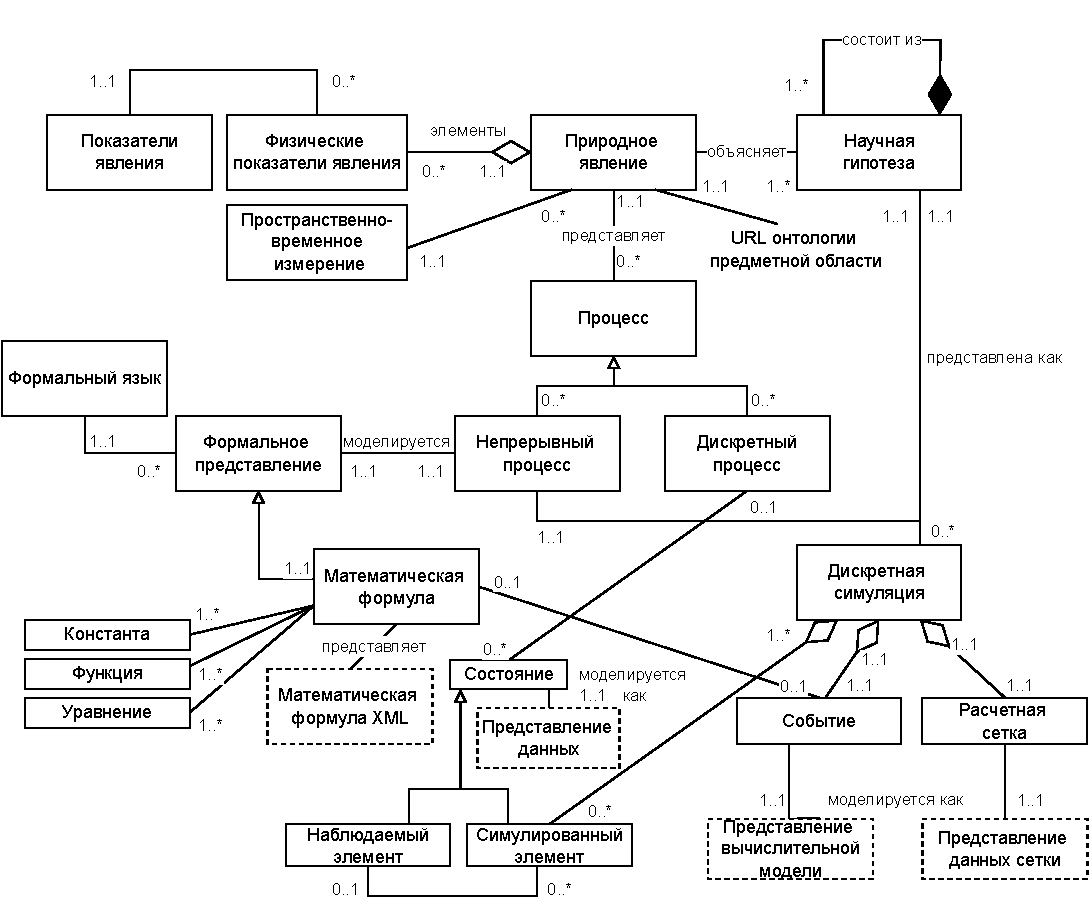
\includegraphics[width=\linewidth]{images/ScHypoConcept}
    \caption{Одна из возможных концептуализаций научной гипотезы.}\label{fig:ScHypoConcept}
\end{figure}

В работе \cite{asgharbeygi2006inductive} представлена математическая формулировка количественных моделей процессов, 
которая обеспечивает формальное кодирование научной моделей в виде системы уравнений, а также неформальное кодирование 
на языке процессов, обозначаемых этими уравнениями. Уточнение модели производится следующим образом. На входе 
необходима изначальная модель; система ограничений, представляющих допустимые изменения начальной модели на языке 
процессов; система базовых (универсальных) процессов, которые могут быть добавлены в начальную модель; наблюдения, 
которым должна соответствовать скорректированная модель. Эти данные обеспечивают эвристический подход, который 
направляет поиск на области пространства модели, которые согласуются с наблюдениями. Алгоритм генерирует множество 
уточненных моделей, которые сортируются по их удаленности от начальной модели и предлагаются вместе со своей 
среднеквадратической ошибкой на тренировочных данных. Расстояние между уточненной и начальной моделью определяется по 
количеству процессов, которые есть в одной, но нет в другой. Состоятельность такого подхода была успешно проверена в 
нескольких областях окружающей среды.

Система формирования гипотез, в основном, однообразна (монотонна) и рассматривается как не вполне подходящая для 
представления знания, в особенности при неполном знании, что часто имеет место в отношении биохимических комплексов. 
В \cite{tran2005knowledge} представлена основанная на знании структура для решения общей задачи формирования гипотез. 
Эта структура была реализована расширением основанной на знании системы <<BioSigNet-RR>>, которая поддерживает 
выработку толерантных представлений и немонотонных логических рассуждений. Главные особенности расширенной системы 
таковы, что они обеспечивают: (1) гладкую интеграцию формирования гипотез с представлением знаний и логическими 
рассуждениями; (2) использование различных ресурсов биологических данных, также как и знаний и опыта человека в целях 
разумной генерации гипотез; (3) поддержку ранжирования гипотез и дизайна экспериментов для проверки гипотез. 
Расширенная система считается прототипом интеллектуального ассистента исследователей – молекулярных биологов.

В проекте «HyBrow» (Hypothesis Space Browser – «Навигатор пространства гипотез») \cite{racunas2004hybrow} гипотезы 
в области биологии представлены как множество предложений исчисления предикатов первого порядка. Если взять сочетание н
абора аксиом, устанавливающих правила, моделирующие известные факты биологии в рамках одной и той же среды, и 
экспериментальные данные, можно обнаружить, что существующая база знаний будет либо противоречить некоторым 
предложениям гипотез, либо подтверждать их, а остальные предложения станут потенциальными открытиями. С получением 
новых экспериментальных данных и формулированием новых правил открытия становятся положительными фактами или 
опровергаются. В случае опровержений должны быть выявлены и удалены из теории, созданной на основе гипотез, те 
правила, которые себя не оправдали. При таком модельно-теоретическом подходе в вопросе подтверждения гипотез 
рассматривается удовлетворение логических импликаций, определенных в модели по отношению к интерпретации. Это может 
быть также применимо к основанным на симуляции исследованиям, где подтверждение выводится из количественного 
анализа "--- сравнения между результатами симуляции и наблюдений \cite{porto2013}. При опровержении или подтверждении 
гипотетических утверждений проект «HyBrow» берет за основу онтологию «OWL» и правила на уровне приложения. 
Проект «HyBrow» обеспечивает разработку гипотез и оценку их на непротиворечивость существующему знанию, а также 
пользуется онтологией гипотез для представления гипотез форме, приемлемой для машин: как отношения между объектами 
(агентами) и процессами \cite{soldatova2011representation}.

Инструмент «HyQue» \cite{callahan2011hyque}, новый этап развития «HyBrow», воспринимает технологии связанных данных 
и использует связанные данные «Bio2RDF», чтобы добавить к «HyBrow» возможности семантической интероперабельности. 
Гипотезы «HyBrow/HyQue» – это предметно-ориентированные утверждения, которые коррелируют с биологическими процессами 
(рассматриваемыми как события) в логике предикатов первого порядка. Гипотезы формулируются как случаи онтологии 
гипотез «HyQue» (HyQue Hypothesis Ontology) и оцениваются с помощью набора вопросов «SPARQL» в сравнении с 
биологически-ориентированными данными «OWL» и «HyBrow». Результаты вопросов оцениваются по некоторой шкале в 
зависимости от того, насколько множество событий соответствует априорным ожиданиям. Оценка по шкале показывает 
уровень поддержки гипотезы данными. Каждое событие оценивается независимо с целью квантифицировать степень поддержки, 
которое оно дает представленной гипотезе. Оценки гипотез привязываются к соответствующим гипотезам как их свойства.

Проект «OBI» (Ontology for Biomedical Investigations – Онтология биомедицинских исследований) 
\cite{brinkman2010modeling} направлен на моделирование дизайна исследования: протоколы, приборы и материалы, 
используемые в ходе экспериментов, а также генерируемые данные. Такие онтологии, как «EXPO» 
\cite{soldatova2006ontology} (см. \cref{fig:EXPO} ) и «OBI», предоставляют возможность документирования всей структуры 
научных исследований: как и с какой целью проведено исследование, какие были сделаны выводы, на какой основе и т.д. 
В результате такой однотипной процедуры по развитию онтологии в работе, заключающейся в получении минимальной 
информации по эксперименту генотипирования (MIGen), рекомендуется использование терминов, определенных в «OBI». 
Использование стандартной или совместимой онтологии для дополнения терминов будет стимулировать междисциплинарный 
доступ к данным и их дальнейшее использование. Для того чтобы сделать исследование более воспроизводимым и допускающим 
повторное использование, предусмотрен сбор возможно большого объема данных.

\begin{figure}[ht]
    \centering
    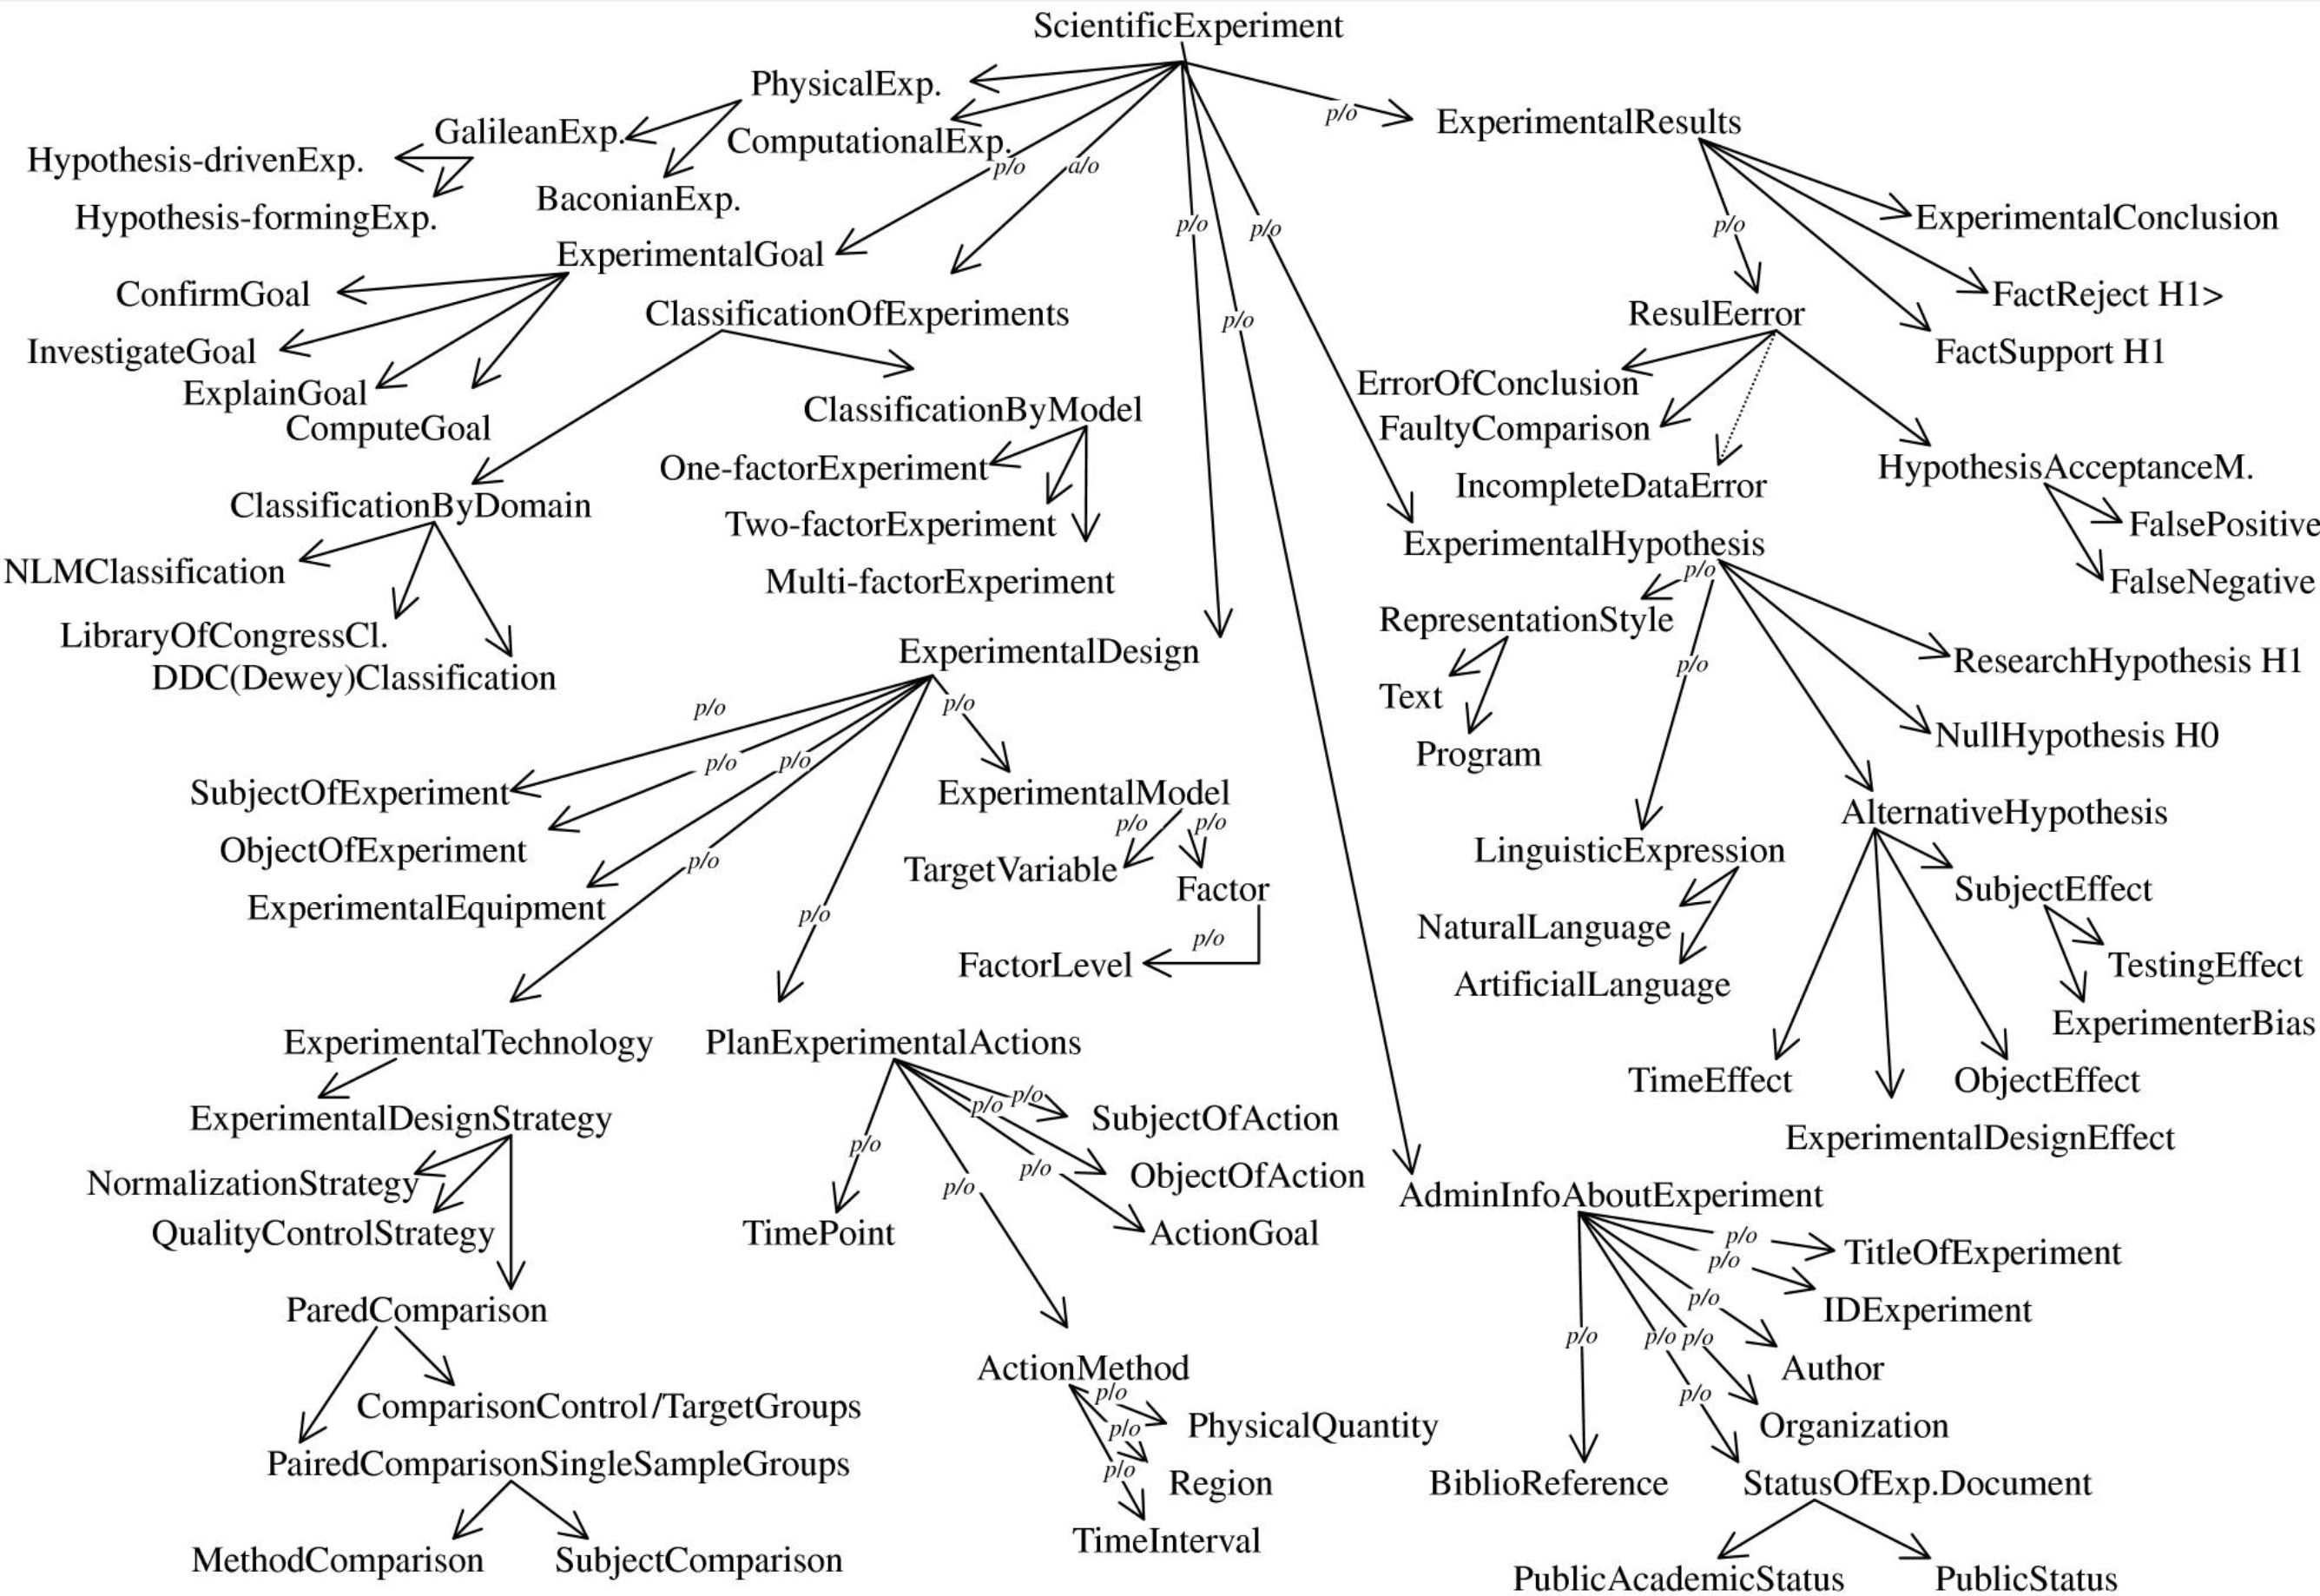
\includegraphics[width=1.0\linewidth]{images/EXPO_onto.png}
    \caption{Фрагмент онтологии научного эксперимента EXPO.}\label{fig:EXPO}
\end{figure}

Моделирование гипотез внедрено в инфраструктуры баз данных, которые развиваются в различных отраслях науки. Один из 
примеров такого рода инфраструктуры имеет наименование «SWAN» (Semantic Web Application in Neuromedicine – 
Семантическое веб-приложение «Нейромедицина») \cite{gao2006swan}. «SWAN» – это проект разработки комплексной 
инфраструктуры знаний для исследовательского сообщества по болезни Альцгеймера. Проект «SWAN» включает в своей 
онтологической модели полный жизненный цикл данных (знаний) в области биомедицинских исследований, в том числе 
организационную поддержку личных данных, генерацию гипотез, ведение экспериментов, организацию лабораторных данных 
и сотрудничество в отношении цифровых препринтов. Общая онтология указывается в «схеме» RDF. Контент проекта «SWAN» 
предназначен для охвата всех этапов процесса «открытия истины» в биомедицинских исследованиях, от формулирования 
вопросов и гипотез, получения экспериментальных данных, совместного с коллегами использования данных, вплоть до полного 
открытия и процесса публикации.

Несколько информационных категорий, которые «SWAN» создает и контролирует определены как подклассы «Утверждения». 
Они включают в себя «Публикацию», «Гипотезу», «Заявку», «Концепцию», «Манускрипт», «Массив данных» и «Аннотацию». 
«Утверждение» может опираться другое «Утверждение» или на любой объект с указанием URL. Например, ученый может 
представить «Комментарий» в отношении «Гипотезы» другого ученого или классифицировать её. Связывание с объектами 
«вне» проекта «SWAN» с помощью URL позволяет использовать информацию «SWAN» в качестве метаданных для организации, 
напр., всех публикаций PDF одного автора, или файлы Excel, в которых зафиксированы данные лаборатории, или все 
веб-сайты инструментов, имеющих отношение к нейробиологии. «Аннотация» может быть как структурированной, так и 
неструктурированной. Структурированность аннотации означает, что она привязана к «Концепции» (с помощью тега или 
термина) к «Утверждению». Неструктурированность аннотации означает привязку свободного текста. 
«Концепции» "--- это узлы вокабуляров, которые также могут быть иерархичными (таксономии).


\section{Основные элементы виртуального эксперимента} \label{sect2_1}

\textit{Определение 1.} \textit{Виртуальный эксперимент} в рамках исследований определяется как 
кортеж $<O, H, M, R, W, C>$, гдe
\begin{itemize}
    \item $O$ "--- это онтология предметной области. Онтология предметной области представляет собой набор понятий и 
            отношений в прикладной области, формально заданных с помощью некоторого языка.
    \item $H$ "--- это набор спецификаций гипотез и взаимосвязей между ними. H является частью онтологии и использует 
            концепции из нее. Вместе они формируют онтологию виртуального эксперимента. Гипотеза "--- это предлагаемое 
            объяснение явления, которое еще предстоит тщательно проверить. 
    \item $M$ "--- это набор моделей. Каждая модель представляет собой набор функций. Каждая модель реализует 
            спецификацию гипотезы. Если модель генерирует ожидаемое поведение какого-либо явления, то говорят, что 
            модель и соответствующая гипотеза подтверждаются наблюдениями.
    \item $R: H \to M$ "--- это отображение из набора гипотез в модели.
    \item $W$ "--- это поток работ. Поток работ представляет собой набор задач, организованных определенными 
            конструкциями (шаблоны рабочего процесса "--- разделение, объединение и т.д.). Каждая задача представляет 
            собой функцию с предопределенной сигнатурой, которая вызывает модели из $M$. Рабочий процесс реализует 
            эксперимент, указывающий, когда следует вызывать каждую модель, соответствующую соответствующим гипотезам. 
    \item $C$ - это конфигурация для каждого запуска эксперимента. Он состоит из полного сопоставления задач 
            рабочего процесса с наборами значений параметров функций.
\end{itemize}

Существует множество возможных реализаций гипотез "--- математические модели, булевы сети, онтологии, предикаты в 
логике первого порядка и т.~д.

Возможными отношениями между гипотезами являются $competes$, который используется для связи конкурирующих гипотез 
и $derived\_by$ для связи двух гипотез, одна из которых использовалась для вывода другой. $derived\_by$ может быть 
использован для формирования решетки гипотез "--- алгебраической структуры с отношением частичного порядка. 
Гипотезы, вытекающие из одной гипотезы, являются атомарными, в противном случае "--- сложными. 
Модель, реализующая гипотезу, должна соответствовать спецификации гипотезы. Если модель генерирует ожидаемое поведение 
какого-либо явления, то говорят, что модель и соответствующая гипотеза подтверждаются наблюдениями.


\section{Жизненный цикл виртуального эксперимента} \label{sect2_2}
Жизненный цикл виртуального эксперимента состоит из четырех этапов и приведен на \cref{fig:lifecycle_ve}. 


\begin{figure}[ht]
    \centering
    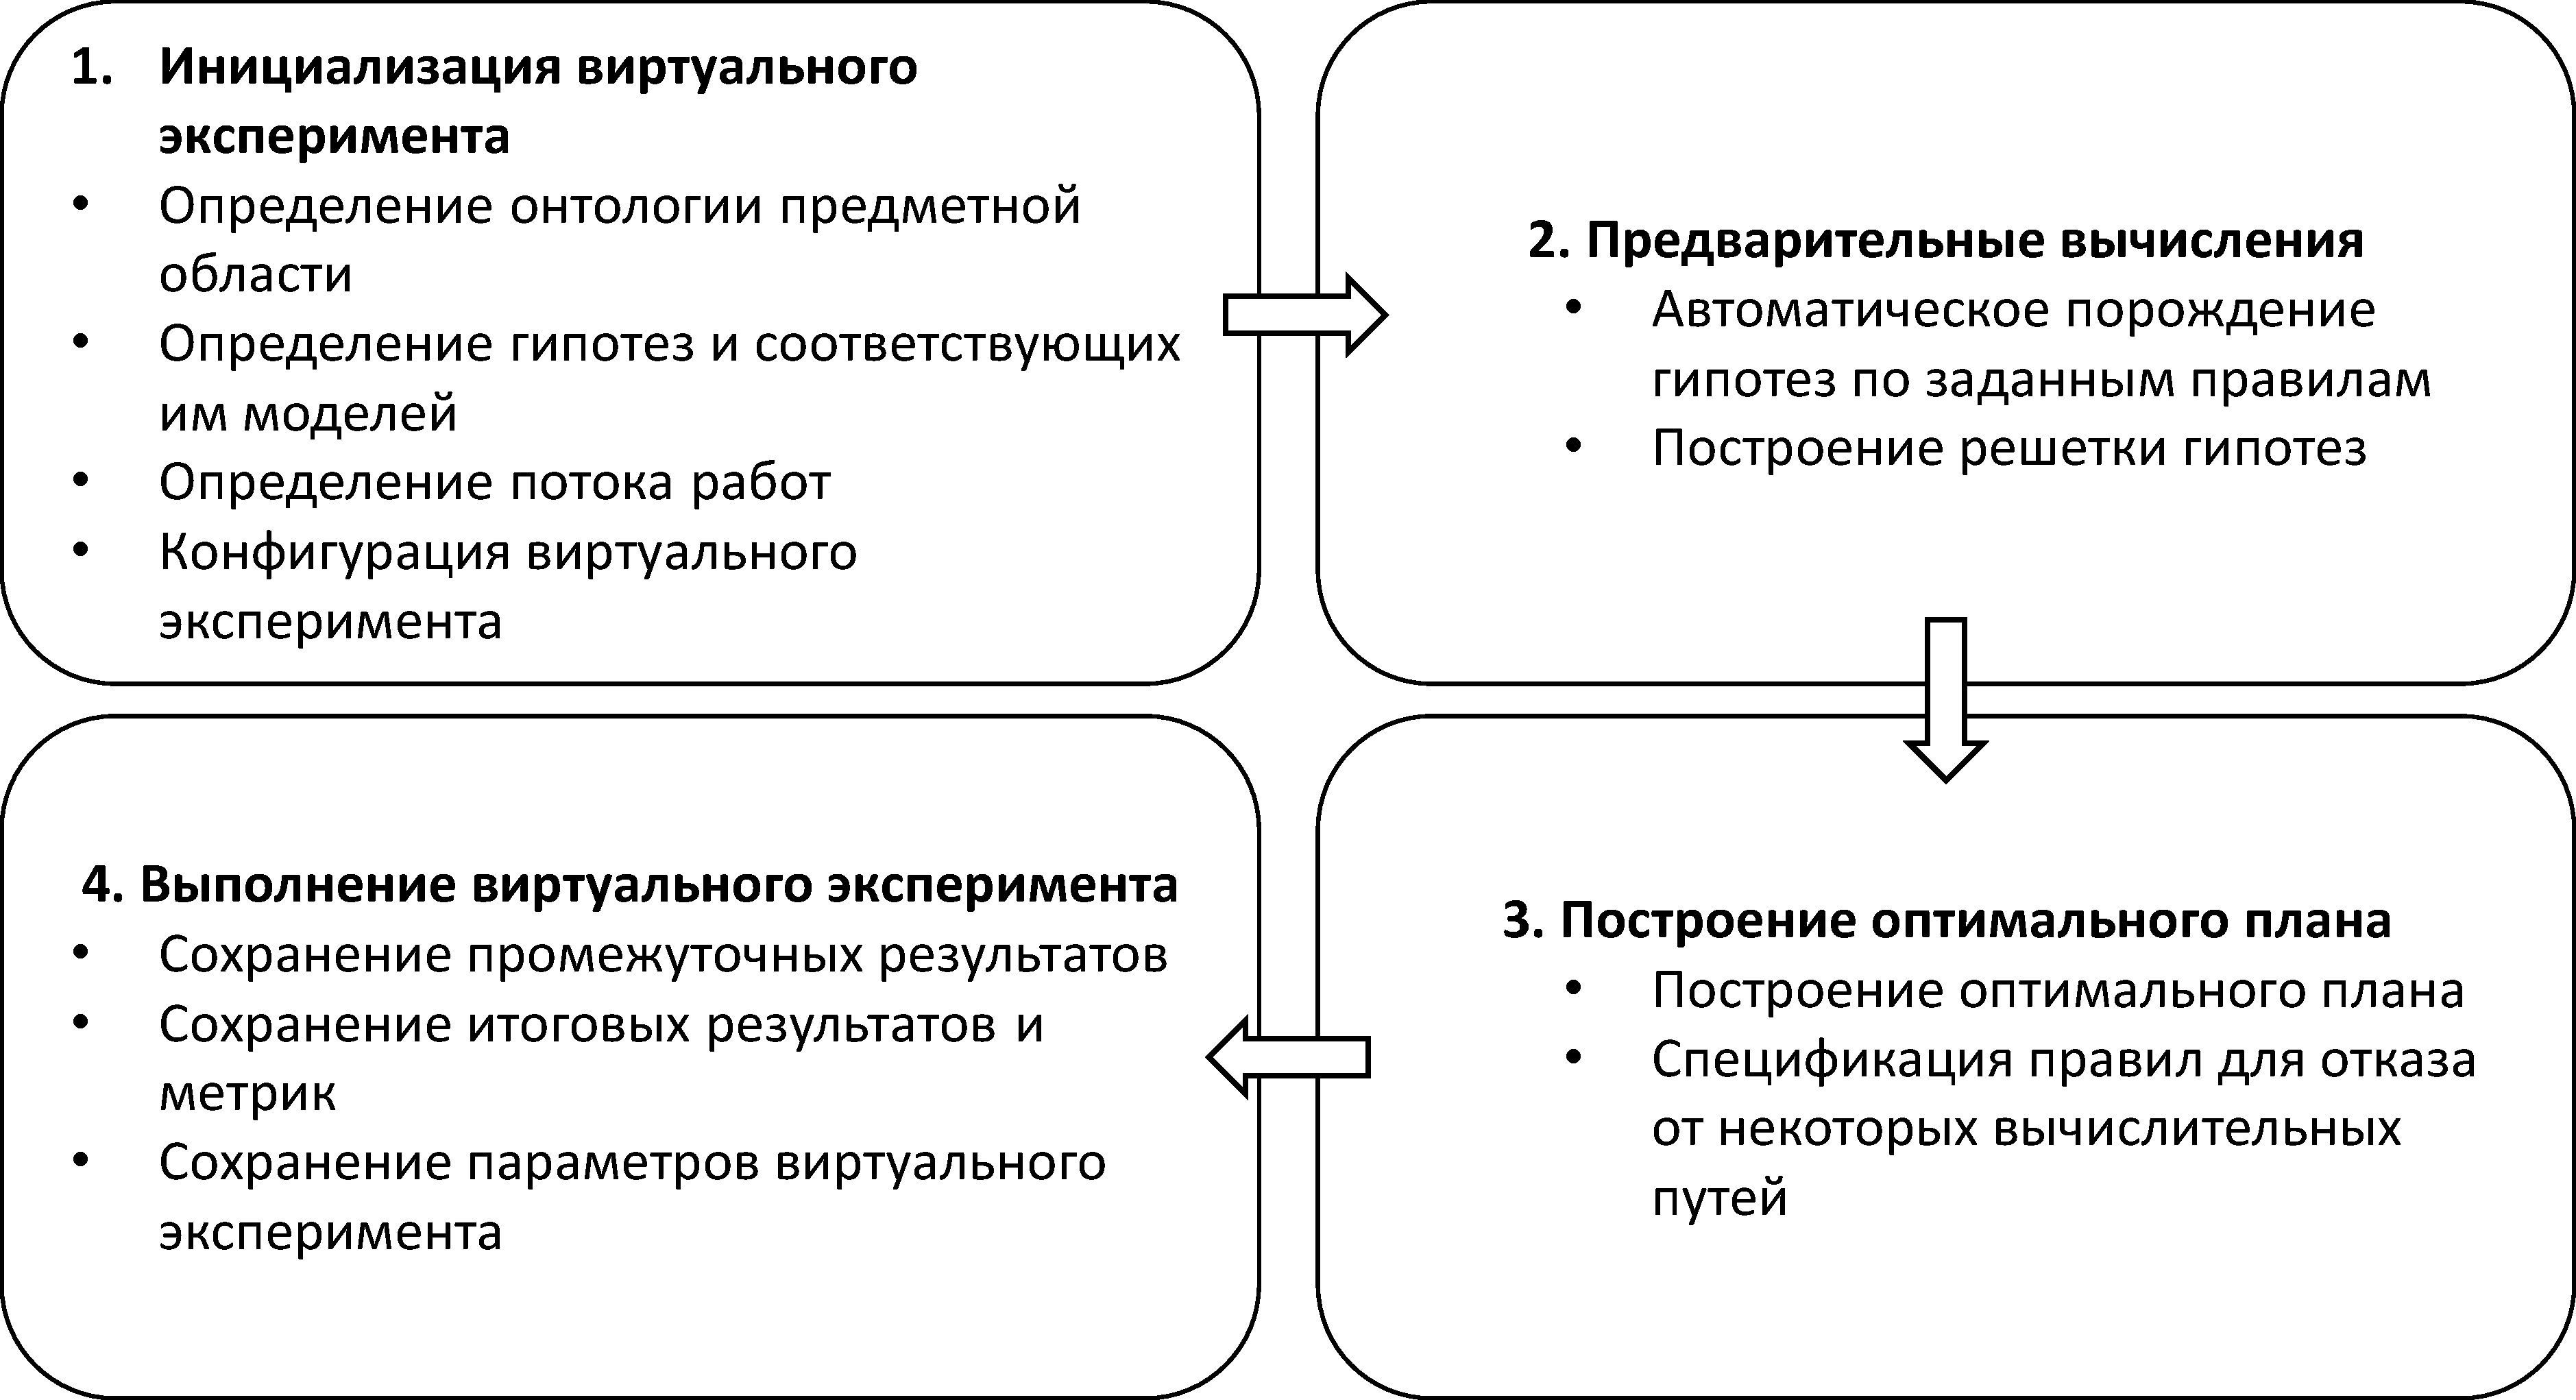
\includegraphics[width=0.9\linewidth]{images/ve_cycle.pdf}
    \caption{Жизненный цикл виртуального эксперимента.}\label{fig:lifecycle_ve}
\end{figure}

На первом этапе происходит инициализация виртуального эксперимента: определение онтологии предметной области, 
определение гипотез и соответствующих им моделей, определение потока работ для исполнения виртуального эксперимента, 
задание конфигурации эксперимента. Поток работ также определяется как направленный ациклический граф. Вершины такого 
графа называются задачами, а каждая задача рассматривается как программа, вызывающая функции, реализующие гипотезы.

На втором этапе по желанию пользователя происходит автоматическое порождение дополнительных гипотез из данных. 
После загрузки виртуального эксперимента в систему происходит автоматическое построение решетки гипотез виртуального 
эксперимента. Используется представление гипотез как специальных структур данных, сочетающих равенства, входящие в 
них переменные и причинно-следственные отображения над ними. Решетка гипотез определяется как направленный ациклический 
граф с вершинами, отвечающими гипотезам. Ребра графа соответствуют отношению завимости между гипотезами, когда 
результат вычислений одной гипотезы используется в вычислениях другой гипотезы. Конструирование решеток отношений 
между гипотезами способствует повышению эффективности управления виртуальными экспериментами, в частности, ускорению 
вычислений с использованием промежуточных результатов, относящихся к независимым гипотезам. 

На третьем этапе происходит построение оптимального плана исполнения нескольких экспериментов. 

На четвертом этапе происходит непосредственное исполнение одного или нескольких виртуальных экспериментов, при этом 
система отслеживает, есть ли в базе данных метаинформации сохраненные результаты исполнения отдельных функций 
эксперимента при заданных параметрах и подставляет их, если совпадение найдено. После исполнения виртуального 
эксперимента результат возвращается эксперту.

По результатам анализа методов манипулирования виртуальными экспериментами был выделен ряд операций для реализации 
в рамках системы по обеспечению полного цикла работы с виртуальным экспериментом. К операциям по работе с виртуальными 
экспериментами, доступным эксперту, относятся добавление, модификация и удаление виртуальных экспериментов, гипотез, 
потоков работ, а также конфигураций экспериментов. Операции, составляющие этап исполнения одного или нескольких 
виртуальных экспериментов, выполняются автоматически для каждой спецификации виртуального эксперимента при ее 
загрузке в систему. 

Промежуточные результаты расчетов, соответствующих вызовам отдельных функций моделей, и оценка их соответствия 
экспериментальным данным сохраняются в базе данных для последующего использования и отслеживания эволюции гипотез и 
моделей виртуального эксперимента.

\section{Решетки гипотез} \label{sect2_3}

Проблема построения структур для одной гипотезы была тщательно изучена в последние годы под разными названиями. 
\noindent Рассматриваются два различных способа нахождения взаимосвязей между гипотезами:
\begin{itemize}
    \item подход <<сверху-вниз>> исходит из анализа математической формы гипотез (обычно в виде набора уравнений);
    \item подход <<снизу-вверх>> исходит из анализа корреляций и зависимостей, присутствующих в данных.
\end{itemize}

Наиболее известным подходом <<сверху-вниз>> является метод, называемый алгоритмом причинного упорядочения 
(COA) \cite{simon1977causal}. Учитывая исследовательскую гипотезу в виде набора математических уравнений, цель 
COA состоит в том, чтобы явно найти отношения асимметрии между переменными уравнений. COA возвращает однозначное 
сопоставление уравнений с переменными для одной исследовательской гипотезы, в то время как взаимодействие нескольких 
гипотез не изучается. Такое отображение определяет ориентированный граф над переменными, где вершины являются 
переменными, а ребра "--- причинно-следственными связями. Переменные, присутствующие в некотором уравнении, 
являются причинно-следственными для зависимой переменной, если в сопоставлении есть запись. 
Сложность COA не учитывается.

В \cite{dash2008note} приводится подробное рассмотрение COA. Авторы формально определяют понятие 
частичного причинного графа и определяют согласованность между ориентированным графом переменных зависимостей 
и частичным причинным графом. Они также вводят основные понятия для выявления причинно-следственных зависимостей, 
скрытых в структуре. Алгоритм возвращает частичное причинно-следственное отображение из разделов набора уравнений 
в разделы одинаковой мощности для набора переменных. Если ровно одно уравнение сопоставляется с одной переменной, 
то сопоставление называется причинным. Показано, что любое действительное полное причинно-следственное отображение 
согласуется с частичным причинно-следственным отображением COA. Вычислительные свойства алгоритмов не обсуждаются. 

Далее в \cite{Goncalves2016} представлен обзор подходов к проблеме причинного упорядочения (COP). COP прямо имеет 
дело со скрытой асимметрией между переменными в заданных наборах математических уравнений. COP исходит из работ по 
моделированию ограничений и рассуждениям \cite{nayak1994causal}. Показано, что COA является NP-трудной проблемой, и 
рекомендуется использовать более эффективный с точки зрения вычислений подход к COP в качестве решения проблемы COA. 
Изображено описание того, как КС связан с проблемой сопоставления гипотез. Вводятся основные определения структур для 
формализации гипотез; представлено предположение о сложности кодирования гипотез из систем уравнений в структуру 
определенного типа. Сложность ограничена $O(|V|*|S|)$, где $S$ "---  структура для набора уравнений $V$ переменных 
с плотностью структуры $S$ (количество появлений переменных) (см. \cref{sect2_3_1} ).

Подход <<снизу-вверх>> реализован в следующих системах: <<Eureqa>> \cite{Schmidt2009}, 
<<Гефест>> (см. \cref{sect1_3_4}), $\Upsilon$-DB (см. \cref{sect1_3_3}).

Eureqa предназначена для вывода символического представления формулы из наблюдений. Авторы демонстрируют, что на основе 
корреляций в наблюдаемых данных отслеживания движения, полученных из различных физических систем, без предварительных 
знаний можно обнаружить законы сохранения геометрии и импульса в виде набора уравнений.

Гефест позволяет проводить виртуальные эксперименты с несколькими конкурирующими гипотезами. Гефест различает два 
разных класса гипотез: введенные исследователем и автоматически выведенные в результате изучения корреляций в данных. 
Все гипотезы сопровождаются вычисленной оценкой точности, например, достигаемым уровнем значимости $p$, исследователю 
показываются только самые высокие оценки для дальнейшей работы. Система не утанавливает взаимосвязи зависимых гипотез 
в виртуальных экспериментах.

В $\Upsilon$-DB предложенный подход дополняет классический статистический подход. Система позволяет работать с двумя 
типами неопределенности "--- теоретической (конкурирующие гипотезы) и эмпирической неопределенностью (альтернативные 
наборы данных). Когда появляются новые данные, этот показатель соответствующим образом корректируется. Моделирование 
обрабатывается как данные, и соответствующие отношения помещаются в ту же базу данных, что и гипотезы. В то же время 
в этих работах не рассматривается вопрос о взаимодействии нескольких гипотез, где доступен рабочий процесс для 
выполнения эксперимента.

\subsection{Построение решетки гипотез} \label{sect2_3_1}
Для определения алгоритма построения решетки гипотез требуются следующие определения из 
\cite{Goncalves2016, kovalev2019constructing}.

\textit{Определение 1.} \textit{Структурой} $S\left(E, V\right)$ называется пара множеств, где $E$ "--- 
это множество уравнений с переменными $V$, так что $|E| \leq |V| $, а так же: 1) в любом подмножестве из $k$ 
уравнений существует не менее $k$ переменных, 2) в любом подмножестве из $k$ уравнений и $r$ 
переменных $\left(k\leq r\right)$, при условии, что значения любых $r-k$ переменных выбираются случайным 
образом, то значения остальных $k$ переменных определяются однозначно.

В данной работе гипотеза $h$ рассматривается как набор уравнений $E_h$ и набор всех переменных $V_h$, указанных 
в $E_h$, так что пара $\left(E_h, V_h\right)$ представляет собой структуру $S\left(E_h, V_h\right)$.

Стоит отметить в определении 1, что структуры состоят из уравнений, а переменные являются их частью только косвенно 
как часть уравнений. Соответственно, все операции множеств, такие как объединение, пересечение и разность, вычисляются 
с использованием уравнений. То есть, если $S(E, V)$ и $S(E',V')$ являются структурами, то $S' \subset S$ , 
когда $E' \subset E$. Определяется дополнительная операция для исключения переменных, т.~е. $T \coloneqq S \div S'$, 
чтобы обозначить структуру $T$, полученную в результате как (1) удаления уравнений $E'$ из $E$, так и 
(2) принудительного исключения переменных $V' = \cup_{f \in E'} Vars(f)$ из $E\setminus	E'$.

\textit{Определение 2.} Пусть $S\left( E, V\right)$ "--- это структура. $S$ является \textit{полной}, если $|E| = |V|$.

\textit{Определение 3.} Пусть $S\left( E, V\right)$ "--- это полная структура. Тогда 
\textit{полное причинно-следственное отображение} над $S$ "--- это биективное отображение $\phi: E\to V$, 
такое что $\forall f \in E$, если $\phi \left( f\right) = x$, то $x \in Vars \left( f \right)$. 
Здесь $Vars \left( f \right)$ "--- это множество всех переменных из уравнений $f \in E$. $|S|$ обозначает число 
появлений переменных в уравнениях, т.~е. $|S\left( E, V\right)| = \sum\limits_{f \in E} Vars\left( f\right)$.


Процедура построения полного причинно-следственного отображения для полной структуры $S\left( E, V\right)$ определена 
в \cite{Goncalves2016}. Вычислительная сложность такого построения ограничена $O\left(|S|*\sqrt{|V|}\right)$.

\textit{Определение 4.} Пусть $S\left( E, V\right)$ "--- это полная структура, где $x_a, x_b \in V$ и $\phi: E \to V$ 
"--- это полное причинно-следственное отображение над $S$. Тогда $C_\phi = \{ \left( x_a, x_b \right) \mid 
\exists f \in E: \phi \left( f \right) = x_b, \text{ } x_a \in Vars\left( f \right) \}$ "--- это множество 
\textit{прямых причинно-следственных зависимостей}. Транзитивное замыкание этого множества обозначается 
$C_\phi^+$ и является набором причинно-следственных зависимостей.  Процедура построения транзитивного замыкания 
для полной структуры $S\left( E, V\right)$ определена в \cite{Goncalves2016}. Вычислительная сложность такого 
построения ограничена $O\left(|S|*|V|\right)$. 

\textit{Определение 5.} Пусть $S\left( E, V\right)$ "--- это структура. Тогда $S$ является \textit{минимальной}, 
если она является полной и нет полной структуры $S'$, такой что $S' \subset S$.

\textit{Определение 6.} Структурная матрица $A_S$ структуры $S\left( E, V\right)$, где $f_1, f_2, \ldots, f_n \in E;
\text{ } x_1, x_2, \ldots, x_m \in V$ "--- это матрица размера $|E| \times |V|$, из нулей и единиц, такая что 
$a_{ij} = 1$, если переменная $x_j \in Vars(f_i)$, иначе~$0$.

\textit{Определение 7.} Решетка гипотез $L$ представляет собой ориентированный ациклический граф, вершины которого 
соответствуют гипотезам с некоторой структурой $S$, а ребра соответствуют отношению $derived\_by$  между гипотезами. 
Отношение $derived\_ by\left(b, a\right)$ означает, что результат вычисления гипотезы $b$ используется при вычислении 
гипотезы $a$.

\textit{Определение 8.} Поток работ $W$ представляет собой ориентированный ациклический граф. Вершины $W$ называются 
задачами. Каждая задача рассматривается как сценарий, вызывающий некоторые функции, реализующие гипотезы. $|W|$ 
обозначает общее количество задач в потоке работ.

Разработанный алгоритм построения решетки гипотез в виртуальных экспериментах представлен в 
\cref{alg:build_lattice}. На входе алгоритм принимает поток работ $W$ и набор гипотез $H$. 
Если поток работ ссылается на гипотезу, которая не представлена в $H$, алгоритм возвращает ошибку. 
В противном случае возвращается решетка гипотезы $L$.  

Задачи потока работ рассматриваются одна за другой в соответствии с порядком, определяемым направлением ребер. 
Для каждой пары гипотез $h_i, h_j$, где $h_i$ упоминается в текущей задаче, а $h_j$ упоминается в некоторой задаче, 
достижимой из текущей задачи, строится транзитивное замыкание для объединения структур соответствующих гипотез. 
После этого все такие транзитивные замыкания объединяются вместе в $C^+$. Структура результирующей решетки $L$ 
соответствует структуре $C^+$. В качестве вершин $L$ включает гипотезы, в которых встречаются переменные из $C^+$. 
Для каждой пары $\left(x_a, x_b\right)$ в $C^+$ \textit{L} включает ребро 
$derived\_by \left(\phi^{-1}\left(x_b\right), \phi^{-1}\left(x_a\right)\right)$.

\begin{algorithm}
    % \SetKwFunction{isOddNumber}{isOddNumber}
    % \SetKwInput{Input}{Input}
    % \SetKwInput{Output}{Output}
    % \SetKwInOut{KwIn}{Input}
    % \SetKwInOut{KwOut}{Output}


    \KwIn{$W$ "--- \texttt{поток работ}, $H$ "--- \texttt{гипотезы}.}
    \KwOut{$L$ "--- \texttt{решетка гипотез}.}

    \For{$h \in V(W)$}{
        \If{$h \notin H$}{
            \textbf{вернуть} \texttt{'Ошибка: гипотезы не найдены'} 
        }
    }
    
    $ C^+ \gets \varnothing $ 

    $\phi \gets \varnothing $ 

    $L \gets \varnothing $

    $ T \gets V\left(W\right) $

    \For{$t \in T$}{
        $T \gets T \setminus t$

        \For{$h_i \in t$}{
            \For{$remain\_t$ \texttt{в} $T$, \texttt{таких что} $remain\_t$ \texttt{достижим из $t$}}{
                \For{$h_i \in remain\_t$}{
                    $S_i \gets $ \texttt{структура для } $h_i$
                    
                    $S_j \gets $ \texttt{структура для } $h_j$
                    
                    \If{$S_i \cup S_{j}$ "--- \texttt{полная}}{ 
                        \texttt{построить транзитивное замыкание } $C_{ij}^+$ \texttt{для} $S_i \cup S_{j}$
                        $C^+ \gets C^+ \cup C_{i}^+ $
                    }
                }
            }
        }
    }

    $\phi \gets $ \texttt{полное причинно-следственное отображение для} $C^+$
    
    $ L \gets L_{inp}$ 
    \For{\texttt{пара} $\left( x_a, x_b \right) \in C^+$}{
    $ V\left(L\right) \gets V\left(L\right) \cup \{\phi^{-1} \left(x_a\right)\}
             \cup \{\phi^{-1} \left(x_b\right)\}$
    
    $ E \left(L\right) \gets E\left(L\right) \cup \{ derived\_by \left(\phi^{-1} \left(x_b\right), 
    \phi^{-1} \left(x_a\right) \right) \} $
    }

    \KwRet{$L$}
    \caption{Построение решетки гипотез}\label{alg:build_lattice}
\end{algorithm}

\textbf{Лемма 1.} Вычислительная сложность алгоритма построения решетки гипотез для потока работ $W$ и набора гипотез 
$H$ ограничена функцией $ O\left( |W|^2 * |S| * |V| * |H| \right)$, где 
$S = \bigcup\limits_{h \in H} S\left(E_h, V_h \right), V = \bigcup\limits_{h \in H} V_h$.

\textbf{Доказательство.} Самой вычислительно сложной операцией алгоритма является построение транзитивного замыкания. 
Так как алгоритм состоит из трех циклов, то максимальное количество операций транзитивного замыкания не превосходит 
$|W|^2*|H|$, где $|H|$ "--- общее количество гипотез. Сложность построения транзитивного замыкания не превосходит 
$O\left(|S|*|V|\right)$, поэтому вычислительная сложность алгоритма построения решетки гипотез ограничена 
$O\left(|W|^2*|H|*|S|*|V|\right)$.

\textbf{Добавление новой гипотезы.} Алгоритм добавления новой гипотезы в существующую решетку гипотез представлен 
в \cref{alg:add_hypothesis}. На входе алгоритм принимает поток работ $W$, существую решетку $L_{inp}$, новую гипотезу 
$H_{add}$. Если поток работ ссылается на гипотезу, которая не представлена в $V\left(L_{inp}\right) \cup h_{add}$, 
алгоритм возвращает ошибку. В противном случае возвращается решетка гипотезы $L$.  

Сначала строится структура $S_{add}$ для добавляемой гипотезы $h_{add}$. Задачи потока работ рассматриваются одна 
за другой в соответствии с порядком, определяемым направлением ребер. Для каждой гипотезы $h_i$, где $h_i$ упоминается 
в текущей задаче, строится соответствующая ей структура. Если объединение этой структуры и структуры $S_{add}$ является 
полным, то строится транзитивное замыкание для объединения структур соответствующих гипотез. После этого все такие 
транзитивные замыкания объединяются вместе в $C^+$. Структура результирующей решетки $L$ соответствует структуре $C^+$. 
В качестве вершин $L$ включает гипотезы, в которых встречаются переменные из $C^+$. Для каждой пары 
$\left(x_a, x_b\right)$ в $C^+$ \textit{L} включает ребро 
$derived\_by \left(\phi^{-1}\left(x_b\right), \phi^{-1}\left(x_a\right)\right)$.

\textbf{Лемма 2.} Вычислительная сложность алгоритма добавления новой гипотезы в существующую решетку гипотез для 
потока работ $W$ и набора гипотез $H$ ограничена функцией $ O\left( |W| * |S| * |V| * |H| \right)$, 
где $S = \bigcup\limits_{h \in H} S\left(E_h, V_h \right), V = \bigcup\limits_{h \in H} V_h$.

\textbf{Доказательство.} Самой вычислительно сложной операцией алгоритма является построение транзитивного замыкания. 
Так как алгоритм состоит из двух циклов, то максимальное количество операций транзитивного замыкания не превосходит 
$|W|*|H|$, где $|H|$ "--- общее количество гипотез. Сложность построения транзитивного замыкания не превосходит 
$O\left(|S|*|V|\right)$, поэтому вычислительная сложность алгоритма построения решетки гипотез ограничена 
$O\left(|W|*|H|*|S|*|V|\right)$.


\begin{algorithm}
    \SetKwFunction{isOddNumber}{isOddNumber}
    % \SetKwInput{Input}{Input}
    % \SetKwInput{Output}{Output}
    % \SetKwInOut{KwIn}{Input}
    % \SetKwInOut{KwOut}{Output}

    \KwIn{$W$ "--- \texttt{поток работ,} $h_{add}$ "--- \texttt{добавляемая гипотеза,} 
        $L_{inp}$ "--- \texttt{существующая решетка гипотез}.}
    \KwOut{$L$ "--- \texttt{решетка гипотез}.}

    \For{$h \in V(W)$}{
        \If{$h \notin V\left( L_{inp}\right) \cup h_{add} $}{
            \textbf{вернуть} \texttt{'Ошибка: гипотезы не найдены'} 
        }
    }
    
    $ C^+ \gets \varnothing $ 

    $\phi \gets \varnothing $ 

    $ T \gets V\left(W\right) $

    $ S_{add} \gets $ \texttt{структура для } $h_{add}$

    \For{$t \in T$}{
        \For{$h_i \in t$}{
            $S_i \gets $ \texttt{структура для } $h_i$
            
            
            \For{$h_i \in remain\_t$}{
                    $S_i \gets $ \texttt{структура для } $h_i$
                    
                    \If{$S_i \cup S_{add}$ "--- \texttt{полная}}{ 
                        \texttt{построить транзитивное замыкание } $C_{i}^+$ \texttt{для} $S_i \cup S_{add}$
                        
                        $C^+ \gets C^+ \cup C_{i}^+ $
                    }
            }
        }
    }

    $\phi \gets $ \texttt{полное причинно-следственное отображение для} $C^+$
    
    $ L \gets L_{inp}$ 
    
    \For{\texttt{пара} $\left( x_a, x_b \right) \in C^+$}{
        $ V\left(L\right) \gets V\left(L\right) \cup \{\phi^{-1} \left(x_a\right)\}
                \cup \{\phi^{-1} \left(x_b\right)\}$
        
        $ E \left(L\right) \gets E\left(L\right) \cup \{ derived\_by \left(\phi^{-1} \left(x_b\right), 
        \phi^{-1} \left(x_a\right) \right) \} $
    }

    \KwRet{$L$}
    \caption{Добавление новой гипотезы в решетку гипотез}\label{alg:add_hypothesis}
\end{algorithm}

\section{Концептуальное представление гипотез, моделей в процессе проведения экспериментов} \label{sect2_4}

Основные понятия и их связи для онтологии виртуального эксперимента представлены на \cref{fig:ve_schema}.

\begin{figure}[h!]
    \centering
    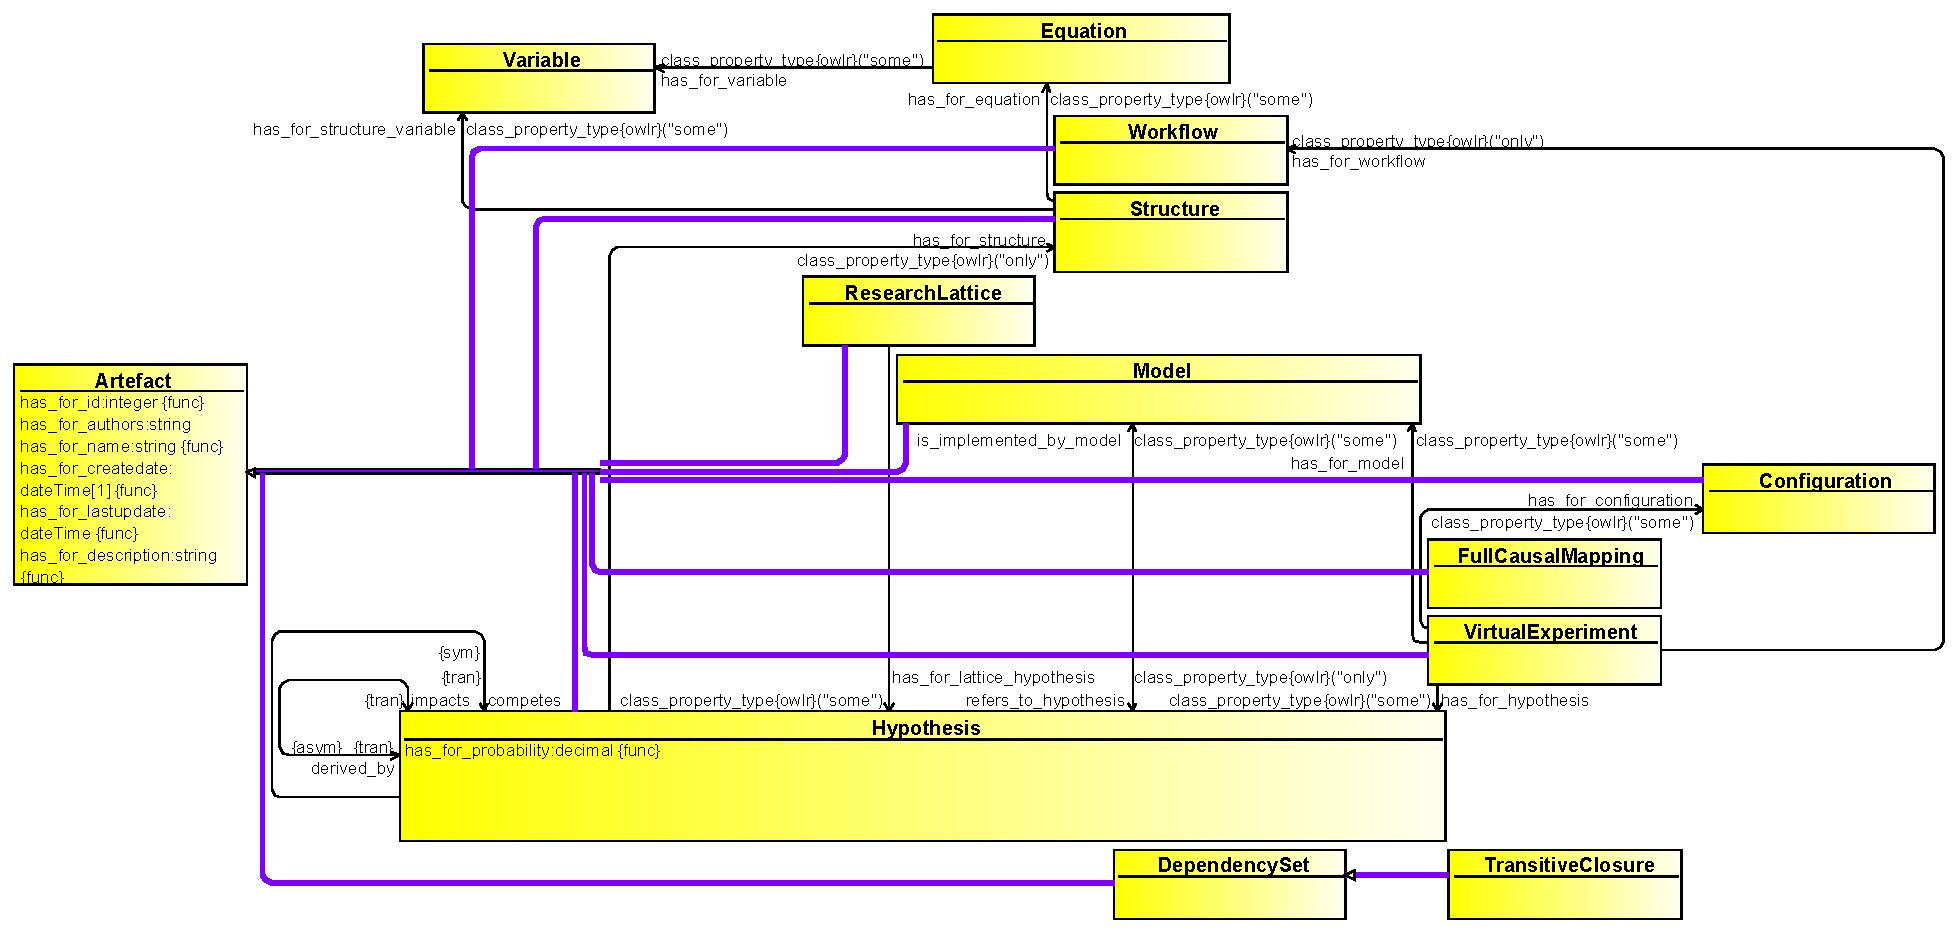
\includegraphics[width=\linewidth]{images/ve_schema2.pdf}
    \caption{Часть онтологии виртуального эксперимента.}\label{fig:ve_schema}
\end{figure}

Определен отдельный ядровой модуль, содержащий классы, соответствующие ключевым понятиям, используемым при работе 
с платформой "--- виртуальный эксперимент, гипотеза, модель, поток работ, конфигурация. Дополнительно определены 
вспомогательные классы переменной, уравнения, структуры, решетки гипотез, полного причинно-следственного отображения, 
множества зависимых переменных и их транзитивного замыкания. 

Модуль использует пакет OwlReady2 \cite{Lamy2017}, который позволяет программировать на Python, ориентированном на 
онтологии, и управлять онтологиями OWL2. Пакет поддерживает такие операции с онтологиями, как загрузка, сохранение, 
изменение, а также рассуждения. Это также позволяет комбинировать методы в Python с классами онтологии, как если бы 
они были объектами Python. Ниже приведен пример определений классов гипотез и моделей:

\begin{ListingEnv}[!h]% настройки floating аналогичны окружению figure
    \captiondelim{ } % разделитель идентификатора с номером от наименования
    \caption{Листинг}\label{lst:hwbeauty}
    % окружение учитывает пробелы и табуляции и применяет их в сответсвии с настройками
    \begin{lstlisting}[language={Python}]
    class has_for_name(Artefact >> str): pass
    class Artefact(Thing):
        is_a = [has_for_name.exactly(1)]
    ...
    class Hypothesis(Artefact): pass
    class Model(Artefact): pass
    class has_for_probability(Hypothesis >> float,
                            DataProperty,
                            FunctionalProperty): pass
    class is_implemented_by_model(Hypothesis >> Model): 
        class_property_type = ["some"]
    class refers_to_hypothesis(ObjectProperty):
        domain              = [Model]
        range               = [Hypothesis]
        inverse_property    = is_implemented_by_model
        class_property_type = ["only"]
    class competes(Hypothesis >> Hypothesis, 
        TransitiveProperty, SymmetricProperty): pass
    class derived_by(Hypothesis >> Hypothesis, 
        TransitiveProperty, AsymmetricProperty): pass
    class impacts(ObjectProperty, TransitiveProperty):
        domain              = [Hypothesis]
        range               = [Hypothesis]
        inverse_propert     = derived_by
    \end{lstlisting}
\end{ListingEnv}%

Гипотеза и модель являются подклассами класса артефактов с одним свойством name (среди прочих). Сюръективное 
отображение из гипотез в модели определяется с использованием свойств объекта 
\textit{is\textunderscore implemented\textunderscore by\textunderscore model} и 
\textit{refers\textunderscore to\textunderscore hypothesis}. Например, домен 
\textit{refers\textunderscore to\textunderscore hypothesis} "--- это модель, а диапазон "--- гипотеза. Отношение 
конкуренции определяется для гипотез как транзитивное и симметричное свойство. \textit{Derived\textunderscore by} 
определяется как транзитивное, но асимметричное свойство. Обратным к \textit{derived\textunderscore by} 
является отношение воздействий.

Гипотеза содержит класс структуры, структура содержит в себе множество уравнений и переменных, а также использует 
классы полного причинно-следственного отображения, множества зависимых переменных и их транзитивного замыкания. 
Решетка гипотез строится по множеству гипотез и потоку работ.

\section{Непротиворечивость виртуального эксперимента}\label{sect2_5}
Для корректного запуска виртуальный эксперимент должен быть \textit{непротиворечивым}. 
Для этого должны выполняться следующие условия:
\begin{enumerate}
    \item Должны быть опредены все элементы виртуального эксперимента $O, H, M, R, W, C$.
    \item Число гипотез должно быть не менее числа задач в потоке работ $|H| \geq |V(W)| $.
    \item Число моделей должно быть не менее числа гипотез $|M| \geq |H|$.
    \item Для каждой гипотезы должна быть опредена реализующая ее модель: $ \forall h \in H: \exists m \in M$ такой, 
            что $h \rightarrow m \in R$.
    
    \item Для каждой задачи потока работ должен существовать набор значений параметров вызываемых функций 
            $ \forall t \in V(W): \exists c \in C$.
    \item После построения решетки гипотез запускается \cref{alg:consistence} проверки отсутствия 
            некорректных зависимостей гипотез в потоке работ.
\end{enumerate}

Если нарушено условие 1), то платформа не сможет запустить выполнение виртуального эксперимента.
При нарушении условия 2) у некоторых задач потока работ будут отсутствовать соответствующие им гипотезы, что не 
позволит корректно построить решетку гипотез. При нарушении условия 3) и 4) некоторым гипотезам не будут 
сопоставлены модели, следовательно их будут невозможно исполнить. Условие 5) гарантирует, что для каждой модели 
существуют параметры ее запуска. Условие 6) необходимо для избежания циклов в графе потока работ, что приведет к 
некорректному построению решетки гипотез Если гипотеза используется в задаче потока работ, то она не может быть 
использована в других задач, достижимых из этой. 

\begin{algorithm}
    \SetKwFunction{isOddNumber}{isOddNumber}
    % \SetKwInput{Input}{Input}
    % \SetKwInput{Output}{Output}
    % \SetKwInOut{KwIn}{Input}
    % \SetKwInOut{KwOut}{Output}

    \KwIn{$W$ "--- \texttt{поток работ}, $L_{inp}$ "--- \texttt{решетка гипотез}.}
    \KwOut{\textit{True} "--- \texttt{некорректные зависимости отсутствуют,} \textit{False} "--- \texttt{иначе}.}

    \textit{correct} $\gets$ \textit{True}

    \For{$t \in V(W)$}{  \Comment{задачи перебираются последовательно}

        \For{$h \in t$}{\Comment{проверяются все гипотезы из задачи}
            \texttt{найти все зависимые $\{h_d\} \in V(L_{inp})$ от $h$ }
            
            \For{\texttt{$remaining\_task$ достижимых из $t$}}{
                \Comment{Эксперимент определен некорректно}

                \If{$\{h_d\} \cap H_t \neq \emptyset\  \alpha\  s.t.\  H_t \in remaining\_task$}{
                    correct $\gets$ \textit{False}   
                }
            }
        }
    }
    \KwRet{correct}
    \caption{Проверка отсутствия некорректных зависимостей гипотез в потоке работ}\label{alg:consistence}
\end{algorithm}


В \cref{alg:consistence} для каждой из задач, которые перебираются последовательно, проверяется, что все гипотезы из 
данной задачи не имеют пересечения зависимых от них гипотез с гипотезами с гипотезами из достижимых задач для данной 
задачи. При нарушении этого условия, возвращается, что эксперимент построен некорректно.

При нарушении любого из этих свойств платформа вернет ошибку определения виртуального эсперимента.

\section{Гипотезы Безансонской модели Галактики}
\subsection{Краткое описание модели Галактики}
Различные астрономические модели существенно опираются на гипотезы. Одной из наиболее впечатляющих является 
Безансонская модель Галактики (\textit{BGM}) \cite{czekaj2014besanccon, robin2003synthetic}, которая разрабатывалась 
в течение более чем 35 лет и представляет собой синтетическую популяционную и структурную модель Млечного Пути. 
Она позволяет астрономам выполнять проверку гипотез относительно формирования звезд, их эволюции, а также химической 
и динамической эволюции Галактики. В результате процесса симуляции можно получать следующее: многомерные гистограммы 
внутренних или наблюдаемых характеристик звезд, каталог псевдонаблюдений, или суммарную светимость в заданной 
фотометрической полосе \cite{czekaj2012galaxy}. Изначально целью \textit{BGM} было не только иметь возможность 
симулировать удовлетворительные подсчеты количества звезд, но и глубже тестировать сценарии эволюции Галактики, 
исходя из допущений о скорости звездообразования (\textit{SFR}), начальной функции масс 
(\textit{IMF}) и звездной эволюции.

С моделью связаны явные и неявные гипотезы. Явные гипотезы "--- обычно некоторые системы уравнений, взятые из 
опубликованных исследований и включенные в модель как её составная часть. Часть явных гипотез включены как входные 
элементы модели, напр., скорость образования звезд, начальная функция масс, эволюционные треки, химическая эволюция, 
модели звездных атмосфер, законы распределения плотности звезд, модель межзвездной экстинкции света.

В модель также включены неявные гипотезы. Например, принято, что ни одна популяция звезд Галактики родилась вне 
Галактики. В модель также включены несколько неявных гипотез об образовании диска и допущения относительно темной 
материи. Как правило, перечислить все неявные гипотезы значительно труднее, поскольку многие из них не описаны в 
публикациях, и их сложно распознать, исходя из кода модели.

BGM включает в себя не только большое количество явных и неявных гипотез, но также и сложных отношений между ними. 
Так, некоторые гипотезы независимы, напр., \textit{IMF} и \textit{SFR}, почему и возможно изменять их независимо. 
С другой стороны, некоторые гипотезы связаны между собой, напр., распределение по возрасту, законы распределения 
звездной плотности и потенциала связаны с зависимостью дисперсии скоростей звезд от их возраста через уравнение 
Больцмана и должны согласовываться. Такого рода зависимости сильно усложняют тестирование модели и поддержание 
её в согласованном состоянии, варьируя различные параметры при настройке модели. Другим примером взаимозависимости 
гипотез являются конкурирующие гипотезы.

\textit{BGM} существенно изменилась за прошедшие 30 лет. Этому способствовало появление результатов изучения новых 
данных, новых технологий и развития методов наблюдения. Пример такой эволюции – модель, разработанная в 2014 г., 
если сравнить её с предыдущими версиями, работает с вариантами \textit{SFR}, \textit{IMF}, эволюционными треками 
и атмосферными моделями. Эти гипотезы вводятся как входные параметры модели, поэтому пользователь может их 
варьировать. Второе усложнение модели – введение двойных звёзд: значительное изменение, поскольку двойные системы 
звёзд составляют примерно 50\% общего наполнения Млечного Пути. Авторы новой версии подчеркивают важность 
понимания взаимозависимости различных гипотез и необходимость инструментов эволюции модели: В практическом плане, 
чтобы построить Галактику из базовых составляющих, нам пришлось реконструировать предыдущую модель и внести 
существенные изменения в построение кода. Это требовало хорошего понимания лежащих в основе отношений между 
всеми предусмотренными компонентами \cite{czekaj2012galaxy}. 
    
В дальнейшем планируется сосредоточиться на обновленной \textit{BGM} \cite{czekaj2014besanccon}, в которой авторы 
привлекают внимание к изучению тонкого диска Галактики и используют Tycho-2 как тестовый набор данных. Набор данных 
Tycho-2 и статистический тест типа $\chi^2$ используются для проверки различных версий этих гипотез, с тем чтобы 
выбирать наиболее пригодные и обновлять модель для лучшего соответствия предоставленным данным. 
Тесты выполнялись путем сравнения количества звезд и цветовых распределений $(B-V)T$ между данными и результатами 
симуляций. Два разных теста были использованы для оценки глобальной соразмерности звездных плотностей и проверки 
формы цветового распределения. 

Другие параметры, которые будут подвергнуты проверке: количества звезд, скорость распространения радиоволн, звездные 
величины, цвета звезд, их собственное движение, параллакс, эффективные температуры, сила тяжести и металличность. 
Авторы используют гистограммы, два критерия согласия (максимальная вероятность и тест $\chi^2$), а также критерии 
Колмогорова---Смирнова и Андерсона---Дарлинга для параметра скорости. 

Параметры одной гипотезы могут быть связаны друг с другом непосредственно с помощью уравнений. Существуют также 
косвенные связи параметров нескольких гипотез, например, параметр \textit{SFR} коррелирует с наклонами \textit{IMF}. 
Это подразумевает, что нельзя было бы дать наилучшее решение для конкретной переменной, не соотнеся ее с другими. 
Таким образом, существует необходимость в поддержке поиска корреляции между гипотезами

Пользователю разрешается изменять не все ингредиенты модели. Это делается потому, что если какая-то гипотеза 
изменяется в модели и никакие дальнейшие корректировки для зависимых гипотез не вносятся, согласованность модели 
нарушается. Кроме того, модель обладает свойством быть самосогласованной, что означает, что при изменении входных 
значений, если это возможно, гипотезы, полученные с помощью измененной, должным образом корректируются, чтобы не 
нарушать фундаментальные уравнения астрономии. Следовательно, производное по отношению должно быть смоделировано. 
Кроме того, системный компонент должен обеспечивать возможность корректировки и калибровки любой гипотезы, 
доступной в модели.

Поскольку количество экспериментов огромно из-за увеличения размера семейства конкурирующих гипотез, теперь не все 
возможные проверяются на всем небе. Изучение способов сокращения количества экспериментов, которые дают наилучшую 
подгонку, и выбора того, когда и если отказаться от дальнейших вычислений эксперимента, является основной частью 
требований к новой системе. Использование информации из эксперимента, проведенного как локально, так и другими 
исследовательскими группами, может быть полезным в достижении этой цели.

В некоторых исследованиях анализа с интенсивным использованием данных подчеркивается роль полос ошибок. Поскольку 
данные в астрономии обычно предоставляются с ошибками, \textit{BGM} использует специальные методы для работы с 
таким типом неопределенности. Компонент, поддерживающий статистические инструменты, который работает с индикаторами 
ошибок, является основным требованием к инфраструктуре

\subsection{Решетка гипотез \textit{BGM}}
Поскольку некоторые составляющие модели находятся в тесной взаимосвязи (такие как IMF, SFR и локальная плотность 
массы), авторы определили конфигурацию модели по умолчанию как сочетание нового набора составляющих, которые 
существенно улучшают согласие с данными Тихо. Поток работ используется для реализации эксперимента \textit{BGM}, 
определяющего, когда следует вызывать каждую модель, которая соответствует связанным гипотезам. Поток работ также 
претерпел изменения по сравнению с первой версией, например, для обработки тонких дисков введены новые действия, 
зависящие от гипотез \textit{IMF} и \textit{SFR}. Это развитие можно отследить только с помощью публикаций. 


Так, были подвергнуты проверке 11 функций IMF, 2 функции SFR, 2 набора эволюционных треков, 3 набора атмосферных 
моделей, 3 значения возраста формирования тонкого диска, 3 набора значений плотности массы звездного объема 
тонкого диска. Пример гипотез для \textit{SFR} приведен на \cref{fig:SFR}.

\begin{figure}[ht]
    \centering
    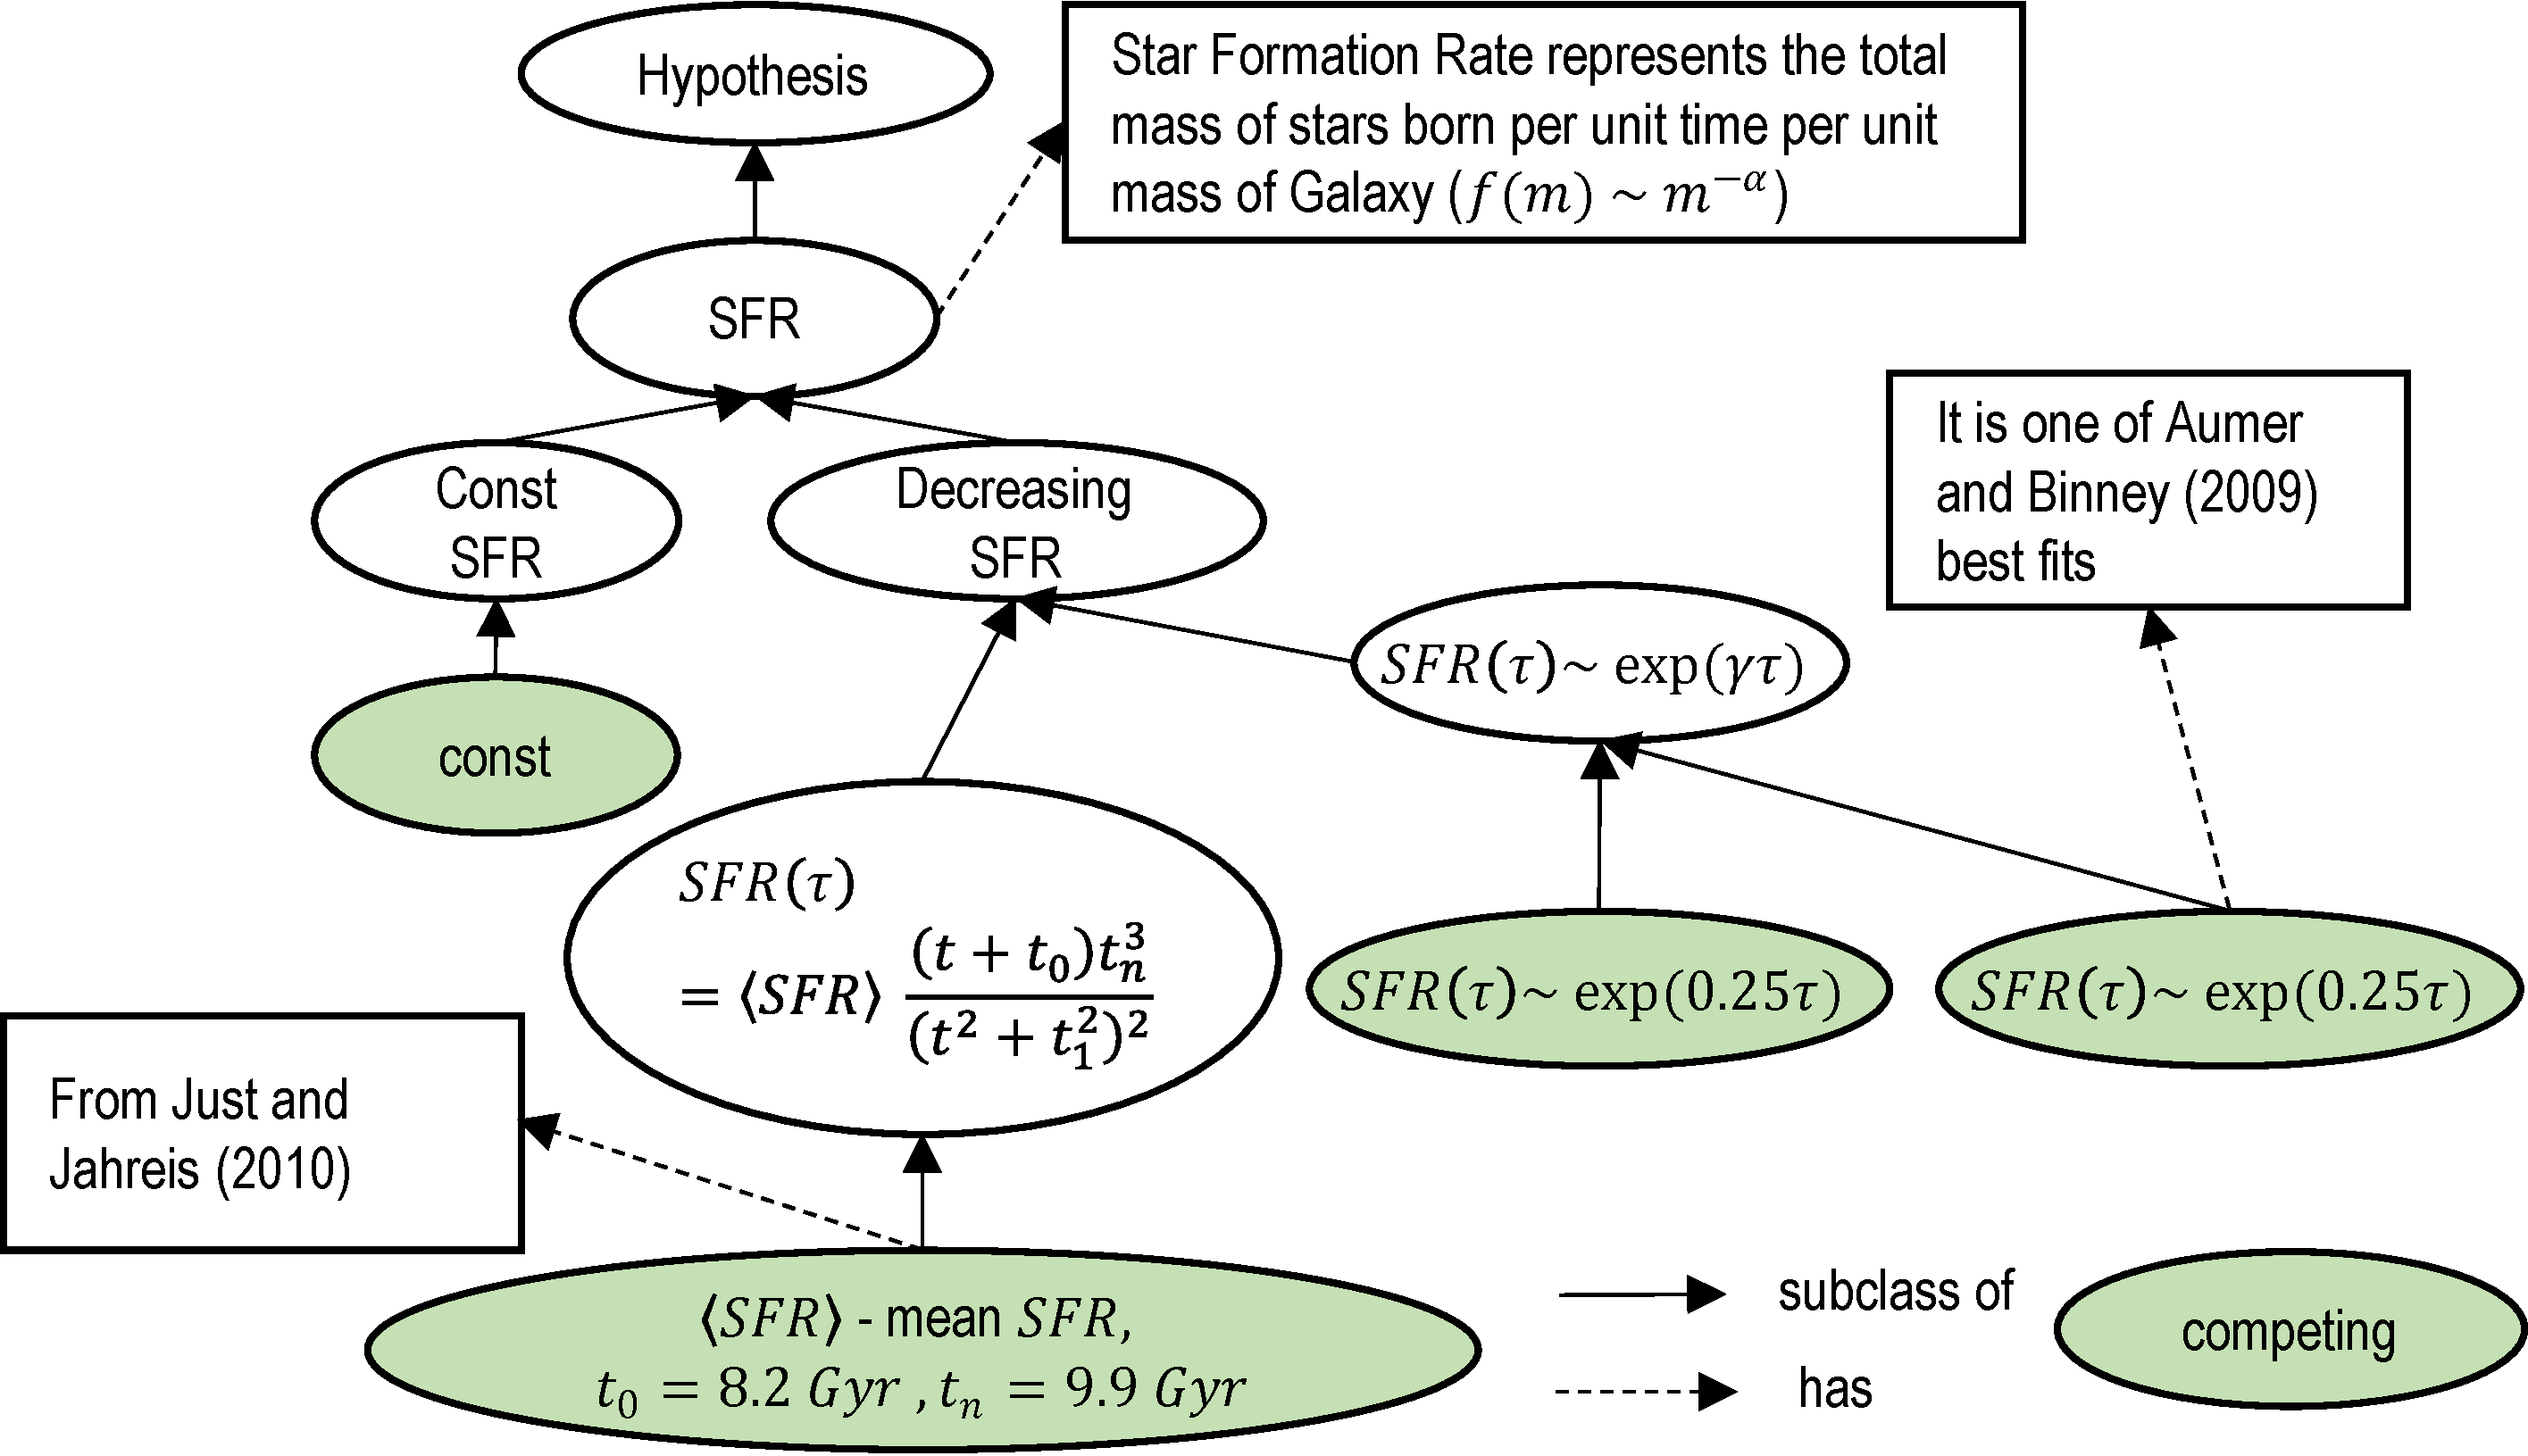
\includegraphics[width=1.0\linewidth]{images/SFR.pdf}
    \caption{Гипотеза SFR для BGM.}\label{fig:SFR}
\end{figure}

\textit{SFR} определяется для семи возрастных ячеек Тонкого диска (структурного компонента Галактики) следующим образом:

\begin{equation}
    SFR(i) = exp(\gamma \times x_c(i)) \times d
\end{equation}

где $x_c(i)$ Э--- возраст в центре ячейки $i$, а $d$ "--- размер этой ячейки. Различными значениями 
$\gamma = \{0.12, 0.25\}$ определяются две конкурирующие гипотезы.

IMF определяется следующим образом:
\begin{equation}
    IMF(m) = m^{-\alpha}
\end{equation}

где $\alpha$ "--- это варьируемый параметр. По мере развития модели в модель вводятся новые значения параметра, 
например, в настоящее время существует 11 различных вариантов для \textit{IMF}.

Локальная объемная плотность $\rho(i)$ "--- это гипотеза для коэффициента нормализации, необходимого для вычисления 
функции звездной рождаемости. Он вычисляется для каждого $i$ на основе предопределенных 
законов плотности и \textit{SFR}.

Функции звездной рождаемости определяются с использованием уравнения:
\begin{equation}
b(m, t)dm dt \approx f\left(SFR\left(i\right), \rho\left(i, SFR\left(i\right)\right)\right) 
\times IMF(m)\Delta m \Delta i
\end{equation}

Стоит отметить, что модель определения массы включает в себя и другие гипотезы 
(полный список гипотез показан на \cref{fig:BGM_lattice}).

В качестве примера мы рассмотрим часть потока работ, которая состоит всего из 
трех последовательных задач (см. \cref{fig:BGM_workflow}). 


\begin{figure}[h!]
    \centering
    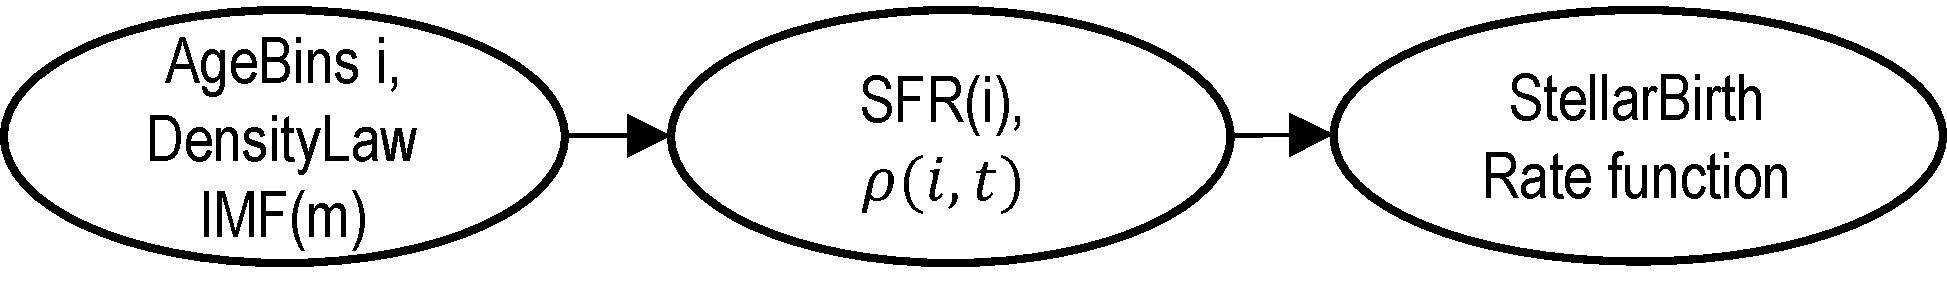
\includegraphics[width=0.7\linewidth]{images/BGM_workflow.pdf}
    \caption{Поток работ для модели определения массы, каждая задача выполняется 
            в соответствии с определенными гипотезами.}\label{fig:BGM_workflow}
\end{figure}

\begin{figure}[ht]
    \centering
    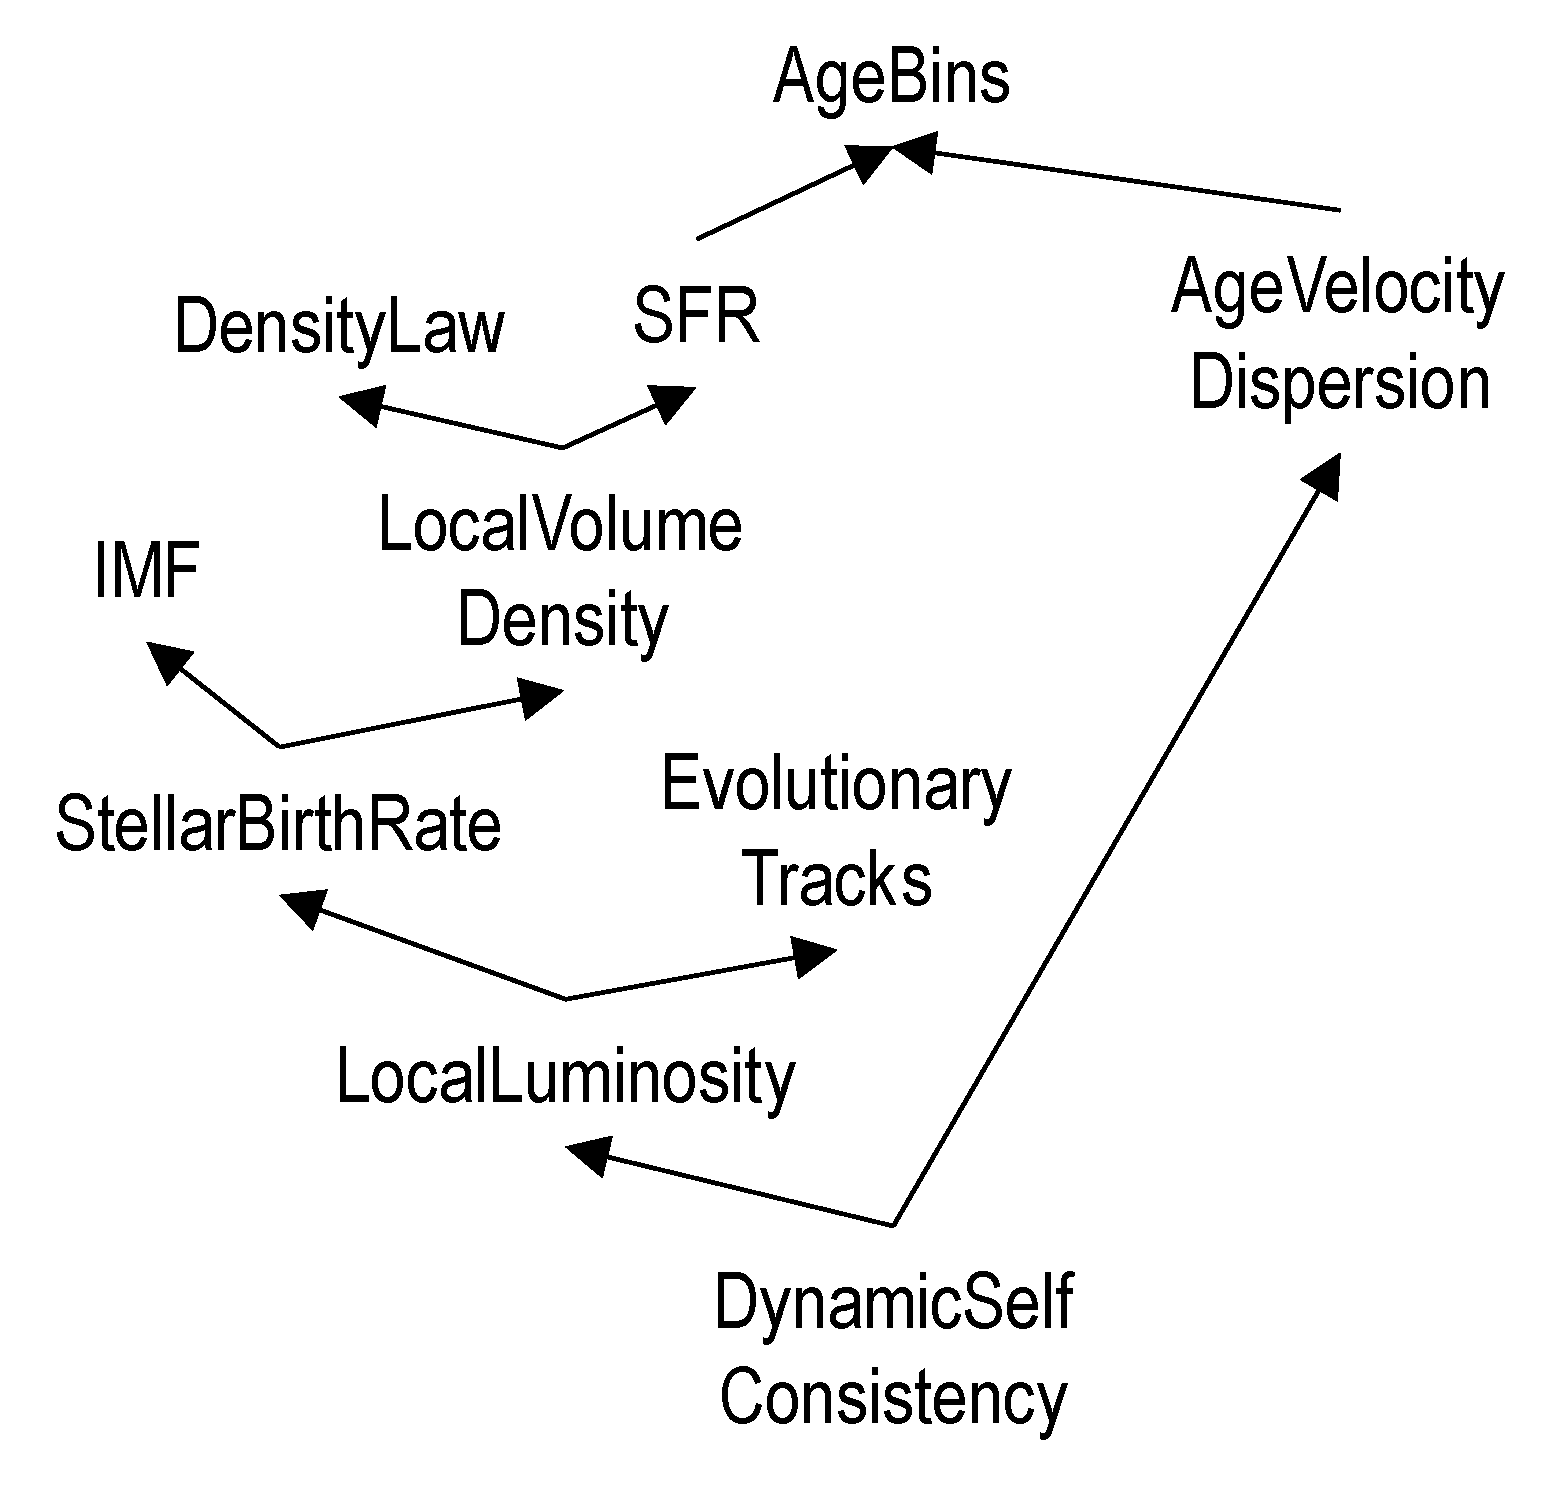
\includegraphics[width=0.6\linewidth]{images/BGM_lattice.pdf}
    \caption{Решетка гипотез  для определения массовой модели с отношением \textit{derived\_by}.}\label{fig:BGM_lattice}
\end{figure}

Первая задача включает гипотезы, соответствующие возрастным ячейкам гипотез, законам плотности и \textit{IMF(m)}. 
Вторая задача состоит из гипотез, соответствующих гипотезам \textit{SFR(i)} и локальной объемной плотности 
$\rho(i, t)$. Третья задача соответствует гипотезе о функции звездной рождаемости.

В соответствии с \cref{alg:build_lattice} строятся структуры для различных пар гипотез. Например, структура 
объединения для возрастных ячеек гипотез и $\rho(i, t)$ является неполной, а структура объединения для возрастных 
ячеек гипотез и $SFR(i)$ является полной. Транзитивное замыкание для возрастных ячеек и $SFR(i)$ 
равно $\{(i, x_c(i)); (i, d)\}$. Транзитивное замыкание индуцирует две вершины \textit{(AgeBins, SFR)} 
и одно ребро \textit{(derived\textunderscore by(AgeBins, SFR))} решетки. Результирующая решетка гипотез 
для модели определения массы изображена на \cref{fig:BGM_lattice}.

Построив решетку гипотез в виртуальном эксперименте, становится возможным формально анализировать и повторно 
использовать результаты частичных вычислений в виртуальном эксперименте. Например, если изменяется только 
гипотеза \textit{IMF}, нет необходимости в повторном вычислении \textit{SFR} или функции локальной объемной плотности.

Разработана концептуальная спецификация виртуального эксперимента для определения модели масс в БГМ, в том 
числе онтология основных понятий предметной области (галактика, тонкий диск, толстый диск, гало, звезда, 
популяция звезд) и спецификации основных гипотез (с использованием языка OWL) и поток работ, формализующий 
виртуальный эксперимент.

На основании анализа предметной области моделирования Галактики (статей, посвященных БГМ и программного 
кода реализации БГМ на языке Фортран 77) выделены основные гипотезы, составляющие модель, например, 
начальная функция масс (IMF) и функция скорости образования звезд (SFR). Начальная функция масс представляет 
собой распределение массы данной популяции звезд и представляется стандартным степенным законом. 
В БГМ функция представлена кусочной функцией с 2 или 3 частями. Существуют ограничения на доступное 
отношение массы к массе Солнца. Представлено 10 различных версий гипотезы, 4 из них являются 2-кусочными 
функциями и 6 из них 3-кусочными.

Определен поток работ виртуального эксперимента, включающий следующие задачи: расчет распределения объемной 
плотности звезд в Галактике (при этом звезды делятся на 7 основных возрастных популяций, для каждой из 
популяций вычисляются параметры распределения), расчет распределения поверхностной плотности звезд для каждой 
популяции, взаимная корректировка объемной и поверхностной плотностей, моделирование параметров звезд 
(например, массы) для каждой из популяций, разбиение звезд на живые звезды и остатки (возможные звёзды, для 
которых возрастное и массовое сочетание противоречат друг другу), пересчет звездного состава тонкого диска с 
использованием уравнения Пуассона, численное решение уравнение Больцмана для популяций звезд с целью проверки 
соответствия модели основным физическим законам.

По представленному потоку работ и гипотезам построена решетка зависимости гипотез с использованием реализованного 
алгоритма. Так, например, гипотеза о рождении новых звезд является зависимой от IMF и косвенно 
от SFR через гипотезу о локальной объемной плотности.

Применяется процедура построения зависимости значения поглощения света в межзвёздной среде от расстояния 
(d) до звезды с определёнными галактическими координатами $(l, b)$ на основе данных многоцветной фотометрии. 
Моделируется наблюдаемый блеск ($m$) в зависимости от спектрального типа звезды ($SpT$), расстояния до неё ($d$) 
и значения межзвездного поглощения ($A_i$) для каждого фотометрического диапазона ($i$). На основе сравнения с 
реальной наблюдаемой яркостью выбирается наиболее подходящий набор моделируемых параметров. Модель позволяет 
получать с приемлемой точностью астрофизические параметры: эффективную температуру, гравитацию, металличность, 
визуальное поглощение и отношение полного поглощения к селективному. Результаты оценки поглощения в заданном 
направлении могут использоваться для выбора адекватной непротиворечивой модели параметров соседних звёзд.


\section{Выводы по главе}\label{sect2_6}



\FloatBarrier
           % Глава 2
\chapter{Платформа для проведения виртуального эксперимента} \label{chapt4}


\section{Архитектура платформы}\label{sect_4_2}
В данном разделе рассмотрены архитектура платформы (\cref{fig:arch}) и то, каким образом компоненты архитектуры 
поддерживают различные этапы деятельности эксперта по проведению виртуальных экспериментов \cite{Kovalev2020_arch}. 
На рисунке пунктирные стрелки обозначают доступ из одного компонента к интерфейсу другого компонента. Программная 
архитектура системы исполнения виртуального эксперимента включает в себя компоненты, поддерживающие различные этапы 
проведения виртуальных экспериментов. В настоящее время архитектура находится в стадии программной реализации.

Разработанный в рамках проекта прототип системы управления виртуальными экспериментами нацелен на объединение 
преимуществ и преодоление недостатков существующих систем. На основании анализа предметной области управления 
виртуальными экспериментами и родственных работ формализовано общее понятие виртуального эксперимента, включающее 
онтологию предметной области, набор спецификаций гипотез и взаимосвязей между ними, набор моделей, реализующих 
гипотезы, поток работ, реализующий эксперимент, конфигурацию (набор значений параметров) эксперимента. Сформулированы 
общие требования к системе для управления виртуальными экспериментами, которым удовлетворяет реализованный прототип. 
Отслеживается эволюция моделей, гипотез и экспериментов. На основании анализа методов формального манипулирования 
виртуальными экспериментами и гипотезами при сохранении непротиворечивости экспериментов для систем с явным 
представлением и использованием гипотез выбраны и реализованы операции управления виртуальными экспериментами и 
их составляющими (гипотезы, модели, их конфигурации). Реализованы методы ранжирования конкурирующих гипотез по 
соответствию наблюдаемым данным на одном или нескольких наборах данных. Предоставляются структуры для хранения 
результатов предыдущих экспериментов, и обеспечиваются запросы к ним. Реализован метод автоматизированного построения 
решеток причинно-следственных зависимостей гипотез в виртуальных экспериментах. Реализован метод порождения гипотез 
из данных, сочетающий обобщенную линейную модель, генетическое программирование и динамическое причинно-следственное 
моделирование. Разработаны и реализованы метод поиска оптимальных параметров гипотез и метод корректной оценки 
соответствия гипотезы исследуемому явлению. Реализован метод повышения эффективности и скорости проведения виртуальных 
экспериментов. Реализованы методы сравнения конкурирующих гипотез, построенных из данных, с теоретическими гипотезами 
из теоретического моделирования или литературы. Реализован подход к интеграции экспериментов, гипотез и данных с 
данными новых наблюдений, симуляций и метаданных экспериментов.

Компонент MetadataRepository представляет собой репозиторий метаинформации (базу данных), предназначенный для хранения 
результатов выполнения виртуального эксперимента с учетом накопления данных о добавлении, модификации и удалении 
гипотез, потоков работ, онтологий и виртуальных экспериментов. Дополнительно в репозитории сохраняются построенные 
зависимости между гипотезами (полученными либо от эксперта, либо автоматически извлеченные) и имеющейся информации 
о корреляции между параметрами как в рамках одной, так и параметров нескольких гипотез.

\begin{figure}[h!]
    \centering
    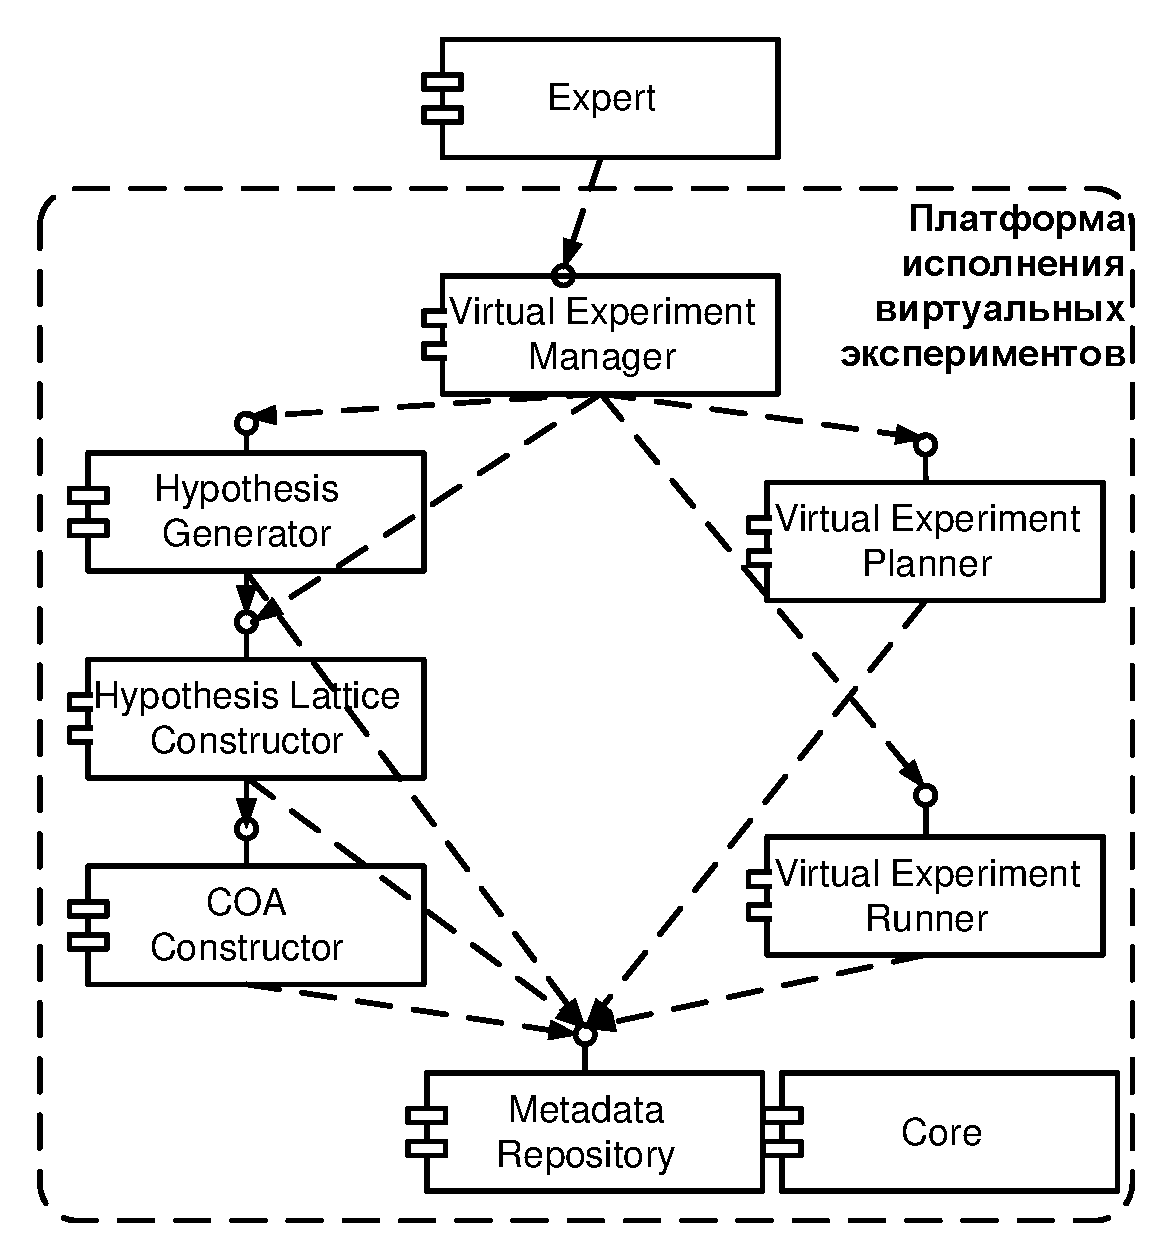
\includegraphics[width=0.7\linewidth]{images/arch_v4.pdf}
    \caption{Архитектура платформы исполнения виртуальных экспериментов.}\label{fig:arch}
\end{figure}

\subsection{Ядровой компонент}
В данном разделе приведено описание ядрового компонента платформы исполнения виртуального эксперимента.
В компоненте представлены методы, которые описывают реализацию подходов из раздела 2 и 
на рис. \cref{fig:core_hypothesis}. 

\begin{figure}[ht]
    \centering
    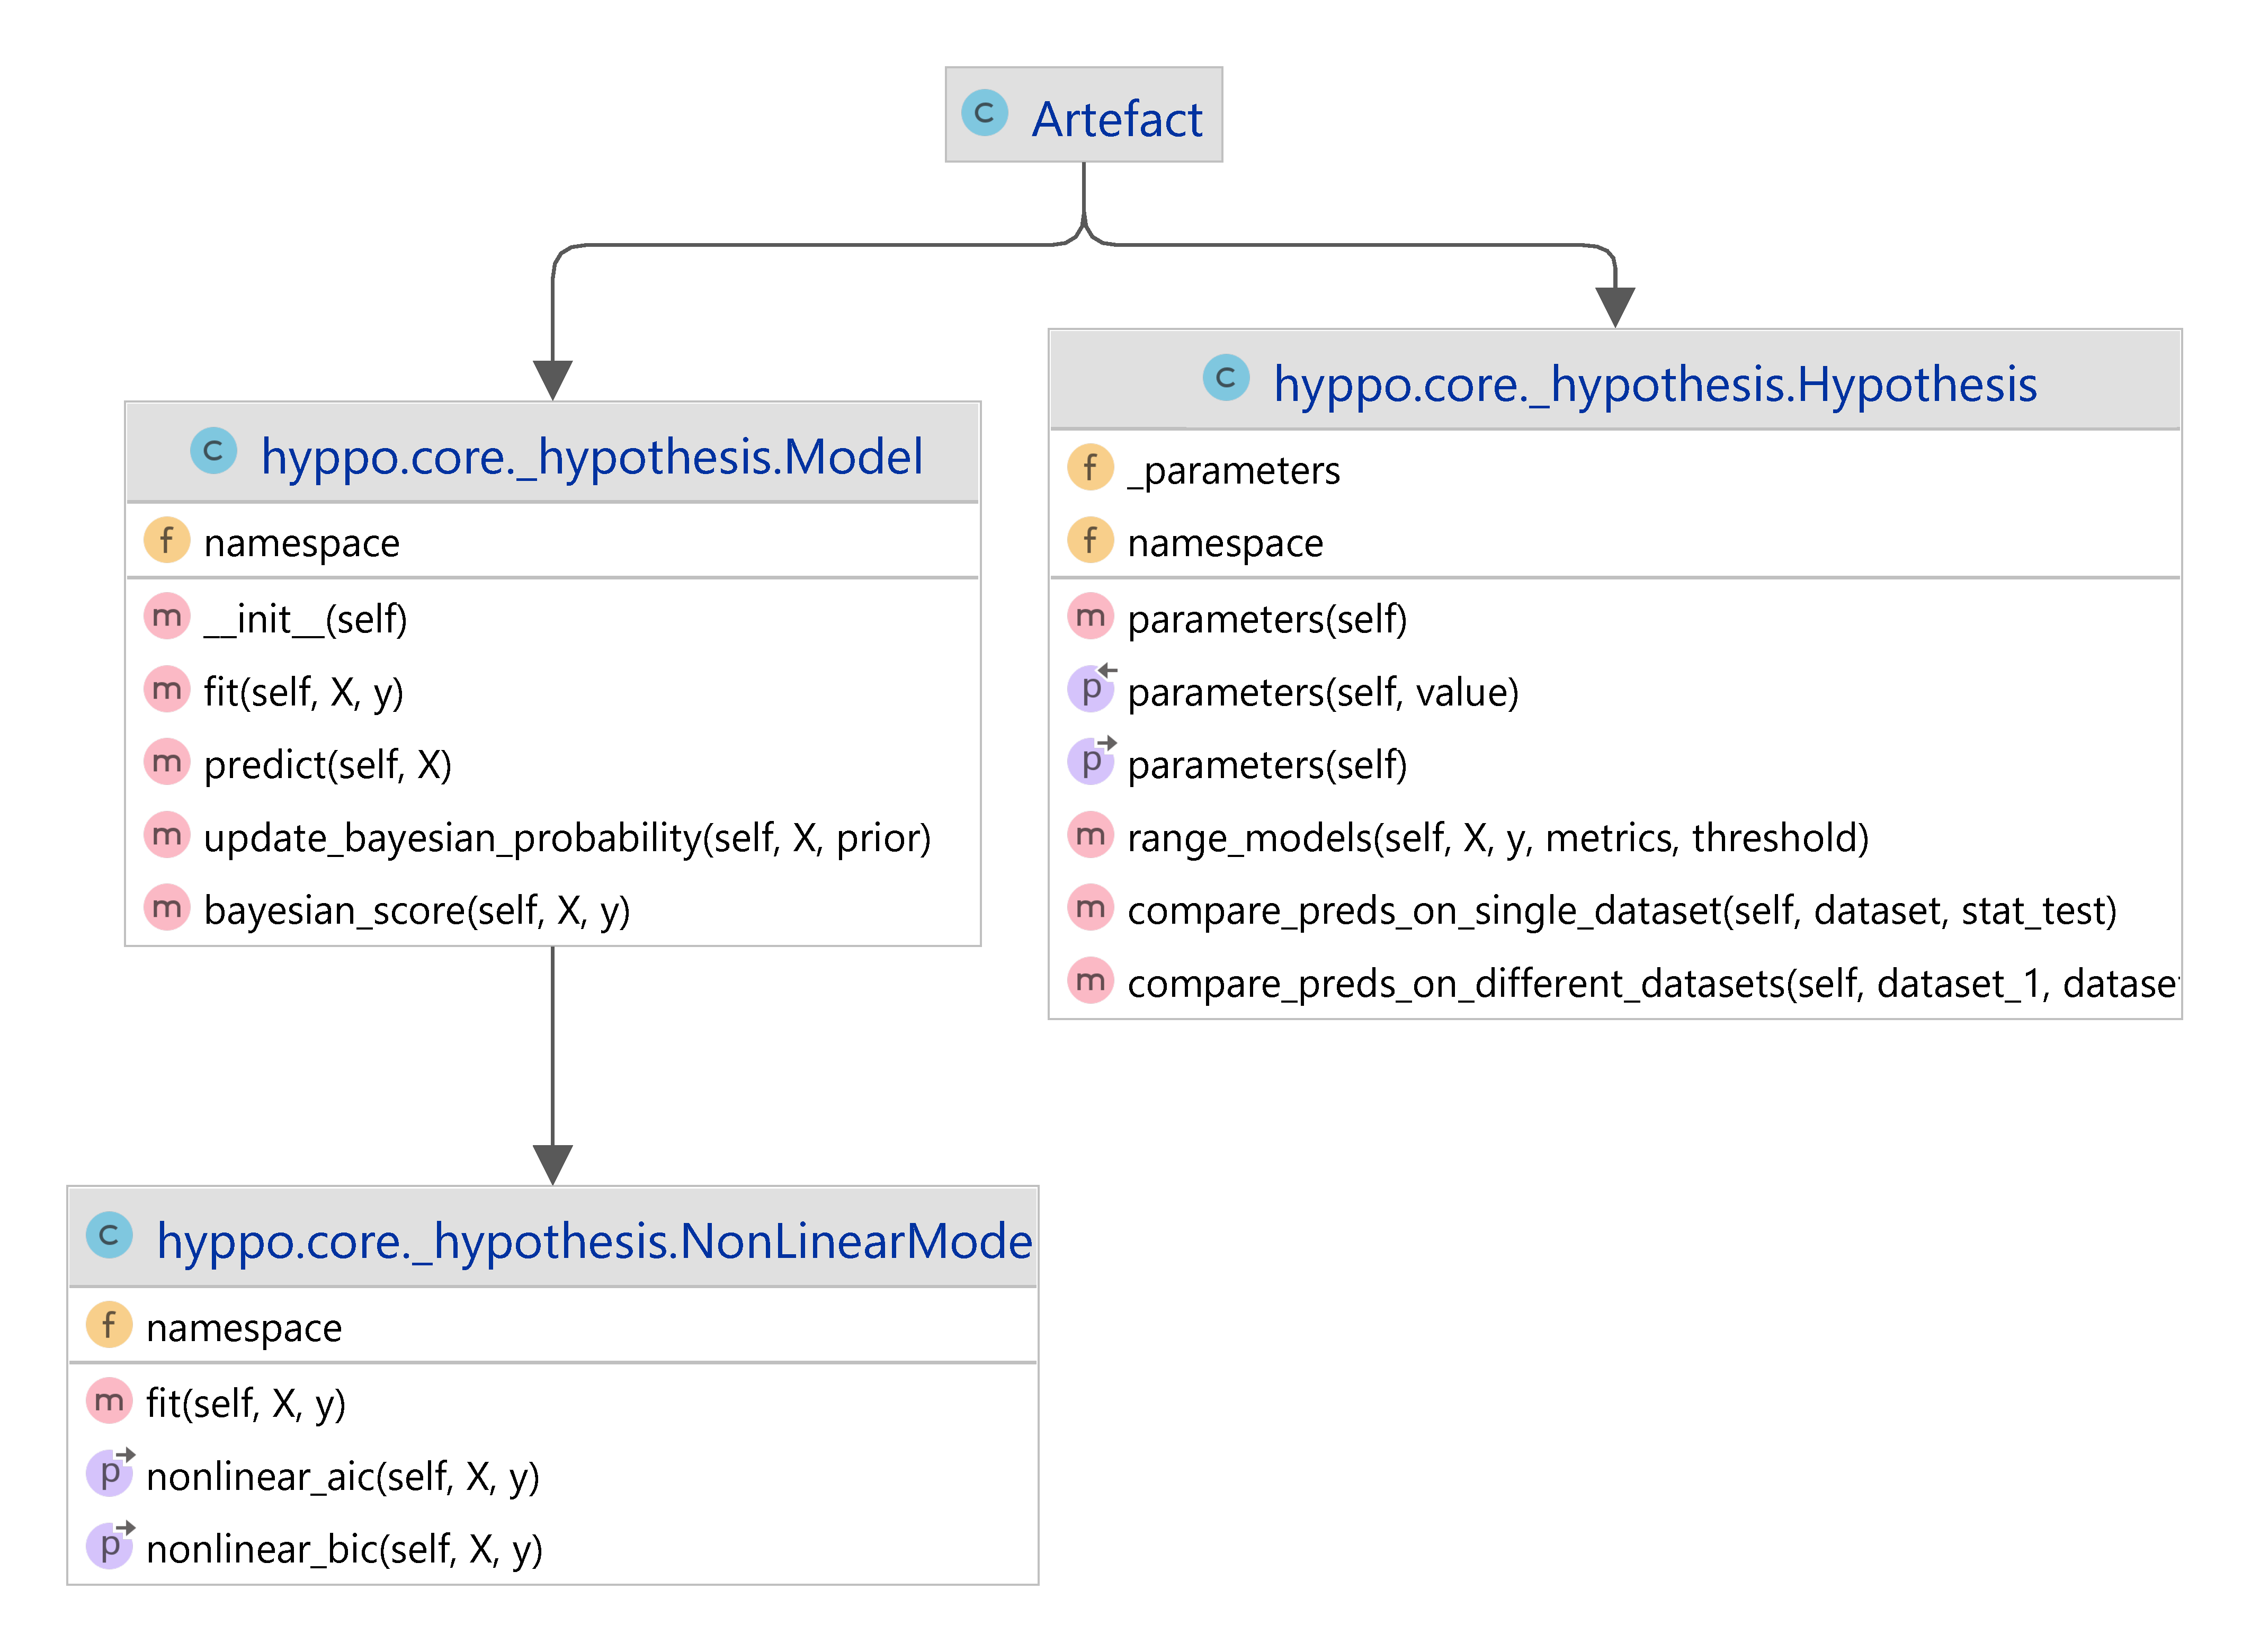
\includegraphics[width=0.7\linewidth]{images/_hypothesis.pdf}
    \caption{Гипотезы и модели в ядровом компоненте.}\label{fig:core_hypothesis}
\end{figure}

\begin{itemize}
   
\item \textit{range\_models(models, dataset, metrics, threshold)} "--- метод для ранжирования моделей по выбранной 
        метрике на выбранном наборе данных. На вход метод принимает набор моделей, которые требуется ранжировать, 
        набор данных, на котором строится выбранная метрика, метрику предсказаний, порог значений для отсечения 
        плохих моделей. В качестве метрик предсказаний могут быть использованы метрики из библиотеки sklearn, 
        например, среднеквадратичную ошибку или коэффициент детерминации, а также информационные критерии, 
        определенные ниже. На выходе метод возвращает ранжированный список моделей с вычисленными метриками.
\item \textit{get\_AIC(model, dataset)} "--- построение информационного критерия Акаике для выбранных модели и набора 
        данных. На вход метод принимает модель и набор данных, на выходе возвращает информационный критерий Акаике.
\item \textit{get\_BIC(model, dataset)} "--- построение Байесовского информационного критерия для выбранных модели и 
        набора данных. На вход метод принимает модель и набор данных, на выходе возвращает 
        Байесовский информационный критерий.
\item \textit{get\_AIC\_nonlinear(model, dataset)} "--- построение информационного критерия Акаике для выбранных 
        нелинейной модели и набора данных. На вход метод принимает модель и набор данных, на выходе возвращает 
        информационный критерий Акаике для нелинейной модели.
\item \textit{get\_BIC\_nonlinear(model, dataset)} "--- построение Байесовского информационного критерия для выбранных 
        нелинейной модели и набора данных. На вход метод принимает модель и набор данных, на выходе возвращает 
        Байесовский информационный критерий для нелинейной модели.
\item \textit{update\_bayesian\_probability(model, dataset, prior\_probability)} "--- метод по построению Байесовской 
        вероятности для выбранной модели на выбранном наборе данных с учетом заданной априорной оценки вероятности. 
\item \textit{compute\_bayesian\_hypotheis\_score(model, dataset)} "--- метод по вычислению байесовской оценки 
        соответствия предсказаний модели наблюдениям.
\item \textit{compare\_models(models, dataset, stattest)} "--- метод сравнения двух моделей между собой на одном 
        наборе данных. На вход метод принимает две модели, набор данных, а также выбранный экспертом статистический 
        тест. На выходе метод возвращает истину, если нельзя отбросить гипотезу о 
        различии предсказаний моделей, иначе ложь. 
\item \textit{compare\_preds\_on\_diff\_sets(models, dataset\_1, dataset\_2, stattest)} "--- метод сравнения моделей 
        между собой на двух наборе данных. На вход метод принимает модель, два набора данных, а также выбранный 
        экспертом статистический тест. На выходе метод возвращает истину, если нельзя отбросить гипотезу о различии 
        предсказаний модели, иначе ложь.
\item \textit{compute\_diff\_dag(models, dataset)} "--- метод для вычисления графа разности двух ориентированных 
        ацикличных графов, построенных по данным входных моделей. На входные модели налагается 
        дополнительное ограничение о линейности. На выходе метод возвращает вычисленный граф разности моделей. 
        Если множество ребер графа пустое, то модели считаются схожими. 
\end{itemize}


\subsection{Компонент управления виртуальным экспериментом}\label{sect_4_2_1}
Компонент VirtualExperimentManager представляет пользователю интерфейс с операциями формального манипулирования 
виртуальными экспериментами и гипотезами. После загрузки виртуального эксперимента в систему его спецификация 
сохраняется в базу данных. Далее, по запросу эксперта происходит вызов компонента автоматического порождения 
гипотез из данных HypothesisGenerator. После этого автоматически происходит вызов компонента 
HypothesisLatticesConstructor для построения решетки гипотез виртуального эксперимента. Далее вызывается компонент 
VirtualExperimentPlanner, отвечающий за построение плана исполнения виртуального эксперимента. Построенный план 
сохраняется в базу данных. Наконец, происходит вызов компонента VirtualExperimentRunner, ответственного за 
непосредственное исполнение виртуального эксперимента. Компонент поддерживает одновременное управление 
несколькими экспериментами.


\subsection{Компонент генерации новых гипотез}\label{sect_4_2_2}

На основании проведенного анализа существующих методов предложен метод порождения гипотез из данных. Основные 
положения метода состоят в следующем. Сначала над данными запускается метод GLM, в результате работы которого 
выделяются такие комбинации переменных, коэффициент при которых значимо отличен от нуля. Одновременно с GLM, для
 этого же набора данных выполняется метод динамического причинно-следственного моделирования. Из полученной для 
 DCM системы уравнений извлекаются только производные от переменных. Далее комбинации переменных GLM и производные 
 переменных метода DCM используются в качестве входных данных для метода генетического программирования. 
 Использование подобной эвристики позволяет значительно сократить время работы метода, при этом увеличивается 
 точность соответствия данным наблюдений. Параллельно запускается метод подбора функции в неявном виде с использованием 
 нейронных обыкновенных дифференциальных уравнений. Вычисленные системы уравнений ранжируются с использованием 
 метрики "--- коэффициента детерминации, эксперту возвращается функция с наибольшей метрикой. При необходимости 
 эксперт может получить формулу зависимости в явном или неявном виде.

Компонент HypothesisGenerator по запросу эксперта обеспечивает автоматическое построение гипотез по данным в виде 
нелинейных функциональных зависимостей. В качестве основного метода используется символьная регрессия, обеспечивающая 
интерпретируемость полученных формул. Эксперту вместе с системой уравнений возвращается оценка качества соответствия 
данным, по которой принимается решение об использовании построенной гипотезы. Компонент реализован в виде модуля на 
языке Python с использованием библиотек pandas, numpy, sympy, deap [5]. Для построения функциональной зависимости 
между переменными в данных используется реализация символьной регрессии на основе генетического программирования 
с арифметическими и тригонометрическими операциями [7]. 



\subsection{Компонент построения причинно-следственного графа}\label{sect_3_1_4}

Компонент COAConstructor позволяет построить причинно-следственный граф зависимостей переменных одной гипотезы. 
Компонент включает механизм вероятностного вывода, позволяющего отследить не только причинно-следственные связи между 
гипотезами, но и неявные зависимости, например, значимые корреляции между параметрами гипотез, не связанных 
причинно-следственными зависимостями. Использование пар значимо коррелирующих переменных позволяет системе указывать 
эксперту, например, на необходимость их совместного изменения. Компонент реализован в виде модуля на языке Python 
с использованием библиотек numpy, latex2sympy, owlready, graphviz, sympy, networkx. Диаграмма классов компонента 
приведена на \cref{fig:base_coa}.

\begin{figure}[h!]
    \centering
    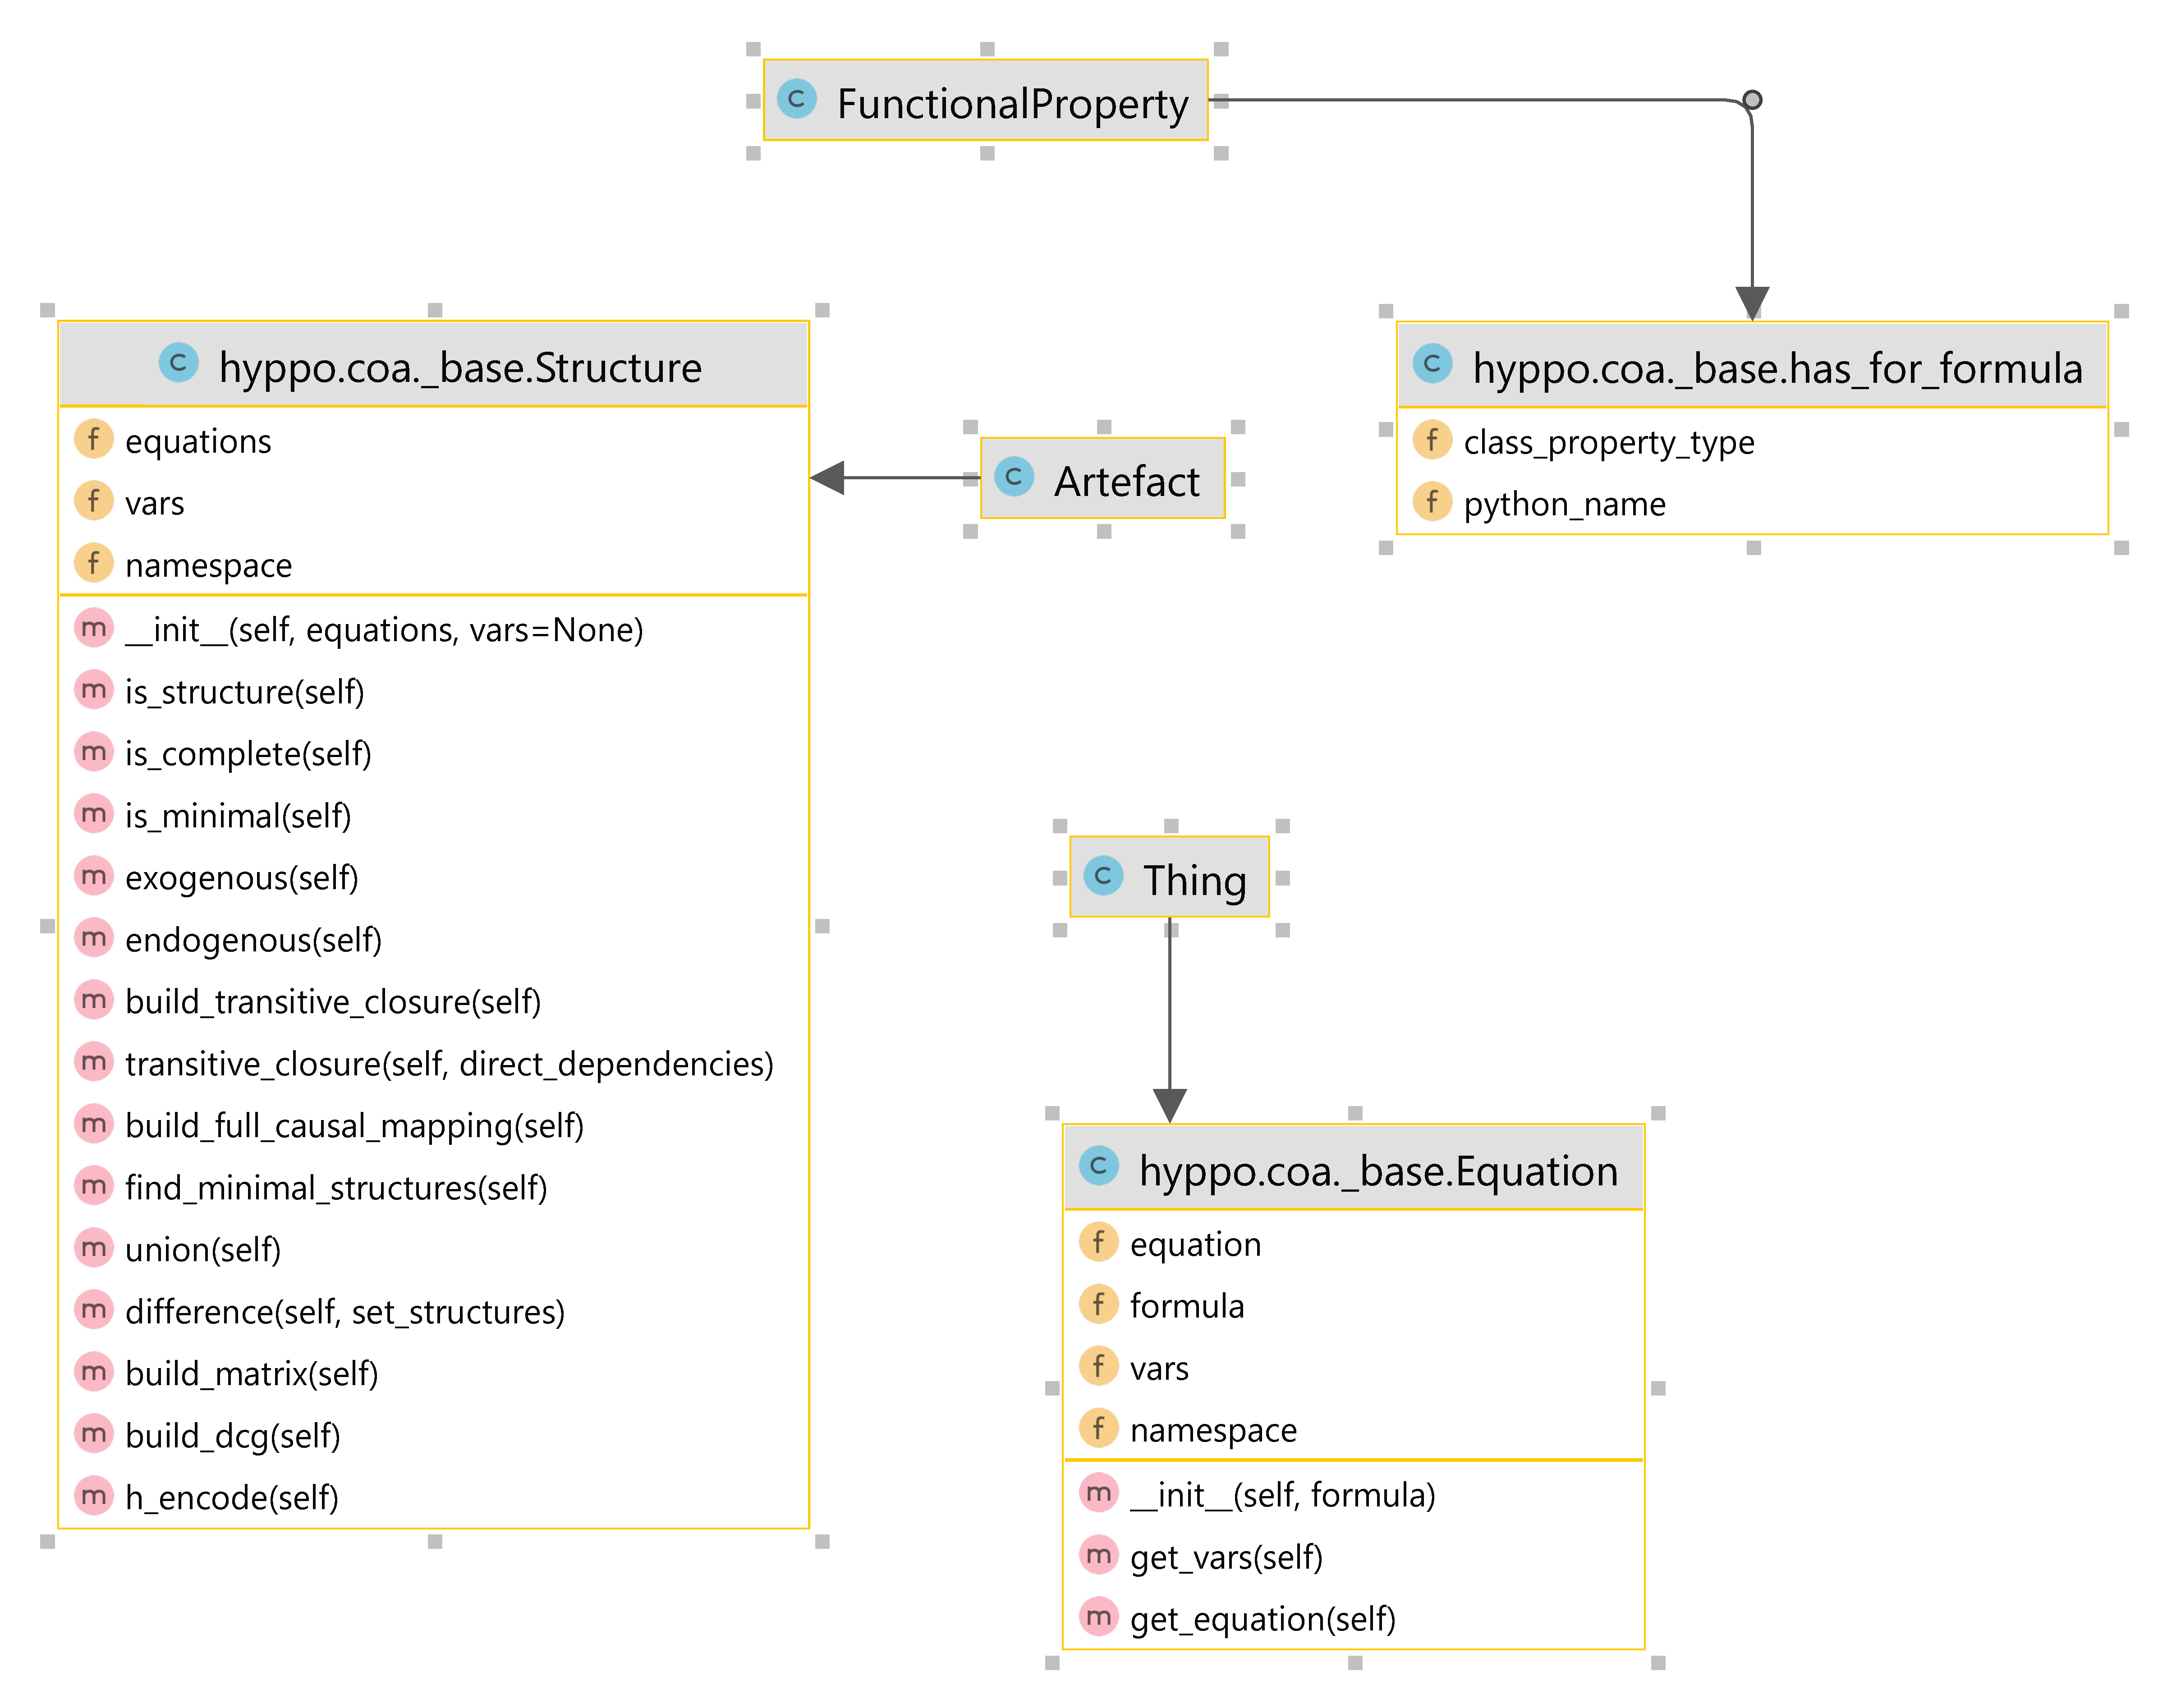
\includegraphics[width=0.9\linewidth]{images/base_coa.pdf}
    \caption{Диаграмма для пакета.}\label{fig:base_coa}
\end{figure}

Компонент включает в себя два класса \textbf{Equation} и \textbf{Structure}. Первый класс представляет собой класс 
уравнений, второй "--- класс структур. Для работы с уранениями и структурами используется их символьное представление.

Методы, входящие в класс \textbf{Equation}:
\begin{itemize}
    \item \textit{get\_vars(self)} "--- метод возвращает множество переменных уравнения.
    \item \textit{get\_equation(self)} "--- метод, преобразующий формулу LaTex в уравнение библиотеки SymPy.
\end{itemize}

Методы, входящие в класс \textbf{Structure}:
\begin{itemize}
    \item \textit{is\_structure(self)} "--- метод возвращает истину, если выполняется определение структуры, 
            иначе "--- ложь. 
    \item \textit{is\_complete(self)} "--- метод возвращает истину, если структура является полной, иначе "--- ложь. 
            Для этого проверяется равенство количества уравнений и количества переменных в структуре.
    \item \textit{is\_minimal(self)} "--- метод возвращает истину, если структура является минимальной, 
            иначе "--- ложь. Для этого проверяется полнота структуры и отсутствие минимальных структур, входящих в нее.
    \item \textit{exogenous(self)} "--- метод возвращает все экзогенные переменные, 
            принадлежащие множеству переменных структуры.
    \item \textit{endogenous(self)} "--- метод возвращает все эндогенные переменные, 
            принадлежащие множеству переменных структуры.
    \item \textit{build\_transitive\_closure(self)} "--- метод возвращает транзитивное замыкание для структуры. 
            Для этого сначала строится полное причинно-следственное отображение. Для каждой пары 
            уравнение-переменная из этого отображения для каждого уравнения извлекаются все его внутренние переменные 
            и удаляется внешняя переменная. Для оставшихся внутренних переменных формируются пары внутренняя 
            переменная - внешняя переменная. Все подобные пары добавляются в множество прямых причинно 
            следственных зависимостей, для которого строится транзитивное замыкание с использованием 
            метода \textit{deps\_transitive\_closure}.
    \item \textit{deps\_transitive\_closure(self, direct\_deps)} "--- метод возвращает транзитивное замыкание множества 
            прямых причинно следственных зависимостей. Для этого строится направленный граф, вершинами которого 
            являются переменные, а ребро из $x_a$ в $x_b$ существует, если во множество прямых зависимостей есть 
            соответствующая пара $(x_a, x_b)$. Далее для каждой вершины формируется пары, где первым элементом является 
            сама вершина, а вторым элементом "--- каждая вершина из множества достижимых вершин. Все пободные пары 
            добавляются в транзитивное замыкание.
    
    \item \textit{build\_full\_causal\_mapping(self)} "--- метод возвращает полное причинно-следственное отображение 
            для данной структуры. Последовательно происходит поиск минимальных подструктур, для которых добавляется 
            пара уравнение-переменные. После этого вычисляется разность между текущей структурой и минимальными и 
            описанная процедура повторяется.
    \item \textit{find\_minimal\_structures(self) } "--- метод возвращает для данной структуры все ее 
            минимальные подструктуры. Метод является рекурсивным. Для каждого элемента из множества всевозможных 
            подможеств подструктур проверяется, являются ли они минимальными. Если элемент является минимальной 
            структурой, то он добавляется в список возвращаемых структур.
    \item \textit{union(self, set\_structures)} "--- метод возвращает объединение структуры со множеством других 
            структур, подаваемых на вход. 
    \item \textit{difference(self, set\_structures)} "--- метод возвращает разность структуру и некоторого 
            множества структур $set\_structures$ . Так как структуры состоят из уравнений, а переменные являются 
            их частью только косвенно, как часть уравнений, соответственно разность вычисляется как разность на 
            множестве уравнений. После этого производится удаление переменных, принадлежащих 
            структурам из $set\_structures$.

    \item \textit{build\_matrix(self)} "--- метод возвращает структурную матрицу для данной структуры. 
            Построение происходит поэлементно, если переменная $x_j \in Vars(f_i)$, то $A_{ij} = 1$, иначе $0$.
    \item \textit{build\_dcg(self)} "--- метод возвращает направленный граф причинно-следственных зависимостей 
            переменных структуры в формате \texttt{dot}. 
    \item \textit{h\_encode(self)} "--- метод возвращает функциональные зависимости для данной структуры.

\end{itemize}



\subsection{Компонент построения решеток гипотез}\label{sect_4_2_3}

Компонент HypothesisLatticesConstructor обеспечивает автоматическое построение решеток гипотез по соответствующим 
им системам уравнений. Компонент загружает из базы данных метаинформации спецификацию потока работ и гипотез. 
Далее системы уравнений, соответствующих гипотезам, из спецификации переводятся во внутреннее представление, 
после чего вызывается компонент COAConstructor для построения причинно-следственного графа зависимостей переменных. 
Решетка гипотез сохраняется в базу данных метаинформации. Компонент реализован в виде модуля на языке Python с 
использованием библиотек pandas, numpy, itertools.
Методы, входящие в компонент:
\begin{itemize}
    \item \textit{build\_lattice(self)} "--- метод возвращает . 
    \item \textit{add\_hypothesis(self, hypothesis)} "--- метод возвращает истину, если структура является полной, 
            иначе "--- ложь. Для этого проверяется равенство количества уравнений и количества переменных в структуре.
    \item \textit{remove\_hypothesis(self, hypothesis)} "--- метод возвращает .
    \item \textit{derived\_by(self, hypothesis)} "--- метод возвращает .
    \item \textit{impacts(self, hypothesis)} "--- метод возвращает .
    \item \textit{is\_correct(self)} "--- метод возвращает .
    
\end{itemize}

Разработанный метод построения решеток гипотез реализован в виде отдельного компонента на языке Python 3.6 с 
использованием библиотеки для научных вычислений scipy и библиотеки поддержки многомерных массивов numpy. Компонент 
включает в себя функции загрузки спецификаций потока работ и гипотез, построения решетки гипотез по набору гипотез и 
потоку работ, вывод и сохранение результатов в локальную файловую систему. Входными данными для алгоритма являются 
спецификации потока работ и гипотез, загружаемые из локальной файловой системы. Реализация алгоритма построения 
решеток гипотез выполнена в отдельной функции, сохранение и отображение решетки гипотез также выполнено 
в отдельной функции.

\subsection{Планировщик виртуальных экспериментов}\label{sect_4_2_5}

Компонент VirtualExperimentPlanner вычисляет оптимальный план исполнения виртуального эксперимента, при этом 
используются решетки гипотез, содержащиеся в репозитории. Это позволяет до проведения виртуального эксперимента 
спланировать оптимальным образом подбор параметров гипотез и отсечь заранее непригодные комбинации параметров. 
Например, уже вычисленные результаты вызова функции модели могут быть повторно использованы в другом виртуальном 
эксперименте, а также могут помочь в исключении виртуального эксперимента, производящего данные, 
не совпадающие с реальными наблюдениями.

\subsubsection{Планирование виртуальных экспериментов}\label{sect_4_4}
Алгоритм планирования исполнения виртуальных экспериментов представлен в .

Использование в виртуальном эксперименте отдельных гипотез и соответствующих им моделей, а также оценка зависимостей 
гипотез друг от друга позволяет сохранять результаты выполнения отдельных частей виртуального эксперимента для их 
повторного использования. Это значительно увеличивает скорость исполнения виртуального эксперимента, повышая 
эффективность использования вычислительных ресурсов.

Основная идея метода повышения эффективности и скорости проведения виртуальных экспериментов состоит в следующем. 
На вход метод принимает спецификацию виртуального эксперимента и построенную для него решетку гипотез. Из множества 
гипотез виртуального эксперимента извлекаются конкурирующие гипотезы, т.е. те, для которых существует несколько 
возможных значений их параметров (гипотезы с разным значением одного параметра конкурируют друг с другом). 
Составляется сетка всевозможных комбинаций таких параметров. Далее с использованием решетки гипотез определяется 
порядок подстановки построенных комбинаций параметров в процессе исполнения виртуальных экспериментов. 
Данный процесс происходит итеративно, при этом на каждом шаге из решетки гипотез убираются гипотезы, не имеющие 
зависящих от себя других гипотез. Если для таких гипотез существуют конкурирующие, то подобная конфигурация 
параметров добавляется в план исполнения виртуального эксперимента. При этом те вызовы функций моделей, параметры для 
которых не изменились, считаются не требующими повторного вычисления, т.е. при непосредственном исполнении 
подставляется уже вычисленный фрагмент виртуального эксперимента. На выходе предоставляется план исполнения 
виртуального эксперимента с указанием порядка подстановки комбинаций параметров, а также частей виртуального 
эксперимента, требующих вызова функций моделей с новыми параметрами.

Метод применим как для работы с новым виртуальным экспериментом, так и для модифицированного виртуального 
эксперимента, например, после добавления в него нового значения параметров для существующей гипотезы. В первом 
случае будет возвращен план исполнения для всего эксперимента, тогда как во втором - только для новых комбинаций 
параметров. При изменении решетки гипотез или спецификации виртуального эксперимента данный метод в системе управления 
виртуальными экспериментами следует вызывать автоматически.
Алгоритм, реализующий разработанный метод, выполнен на языке Python 3.6 с использованием библиотек NumPy, SciPy, 
Pandas. Реализация выполнена в виде отдельного модуля. Для хранения результатов проведенных экспериментов используется 
реляционная база данных.


\subsubsection{Отказ от некоторых вычислительных маршрутов}\label{sect_4_3}



\subsection{Компонент исполнения виртуальных экспериментов}\label{sect_4_2_6}

Компонент VirtualExperimentRunner запускается для непосредственного исполнения виртуального эксперимента. 
Из репозитория метаинформации загружаются спецификация виртуального эксперимента и дополнительно построенные 
решетка гипотез и план исполнения виртуального эксперимента. Исполнение происходит в соответствии с планом, при 
этом система использует сохраненные результаты исполнения части виртуального эксперимента (при их наличии в 
репозитории метаинформации). Используя спецификацию моделей виртуального эксперимента, компонент осуществляет 
вызов соответствующих функций, а затем собирает полученные данные от них. Результаты исполнения виртуального 
эксперимента сохраняются в базу данных метаинформации.


\subsection{Репозиторий метаинформации}\label{sect_4_2_7}

\begin{figure}[h!]
    \centering
    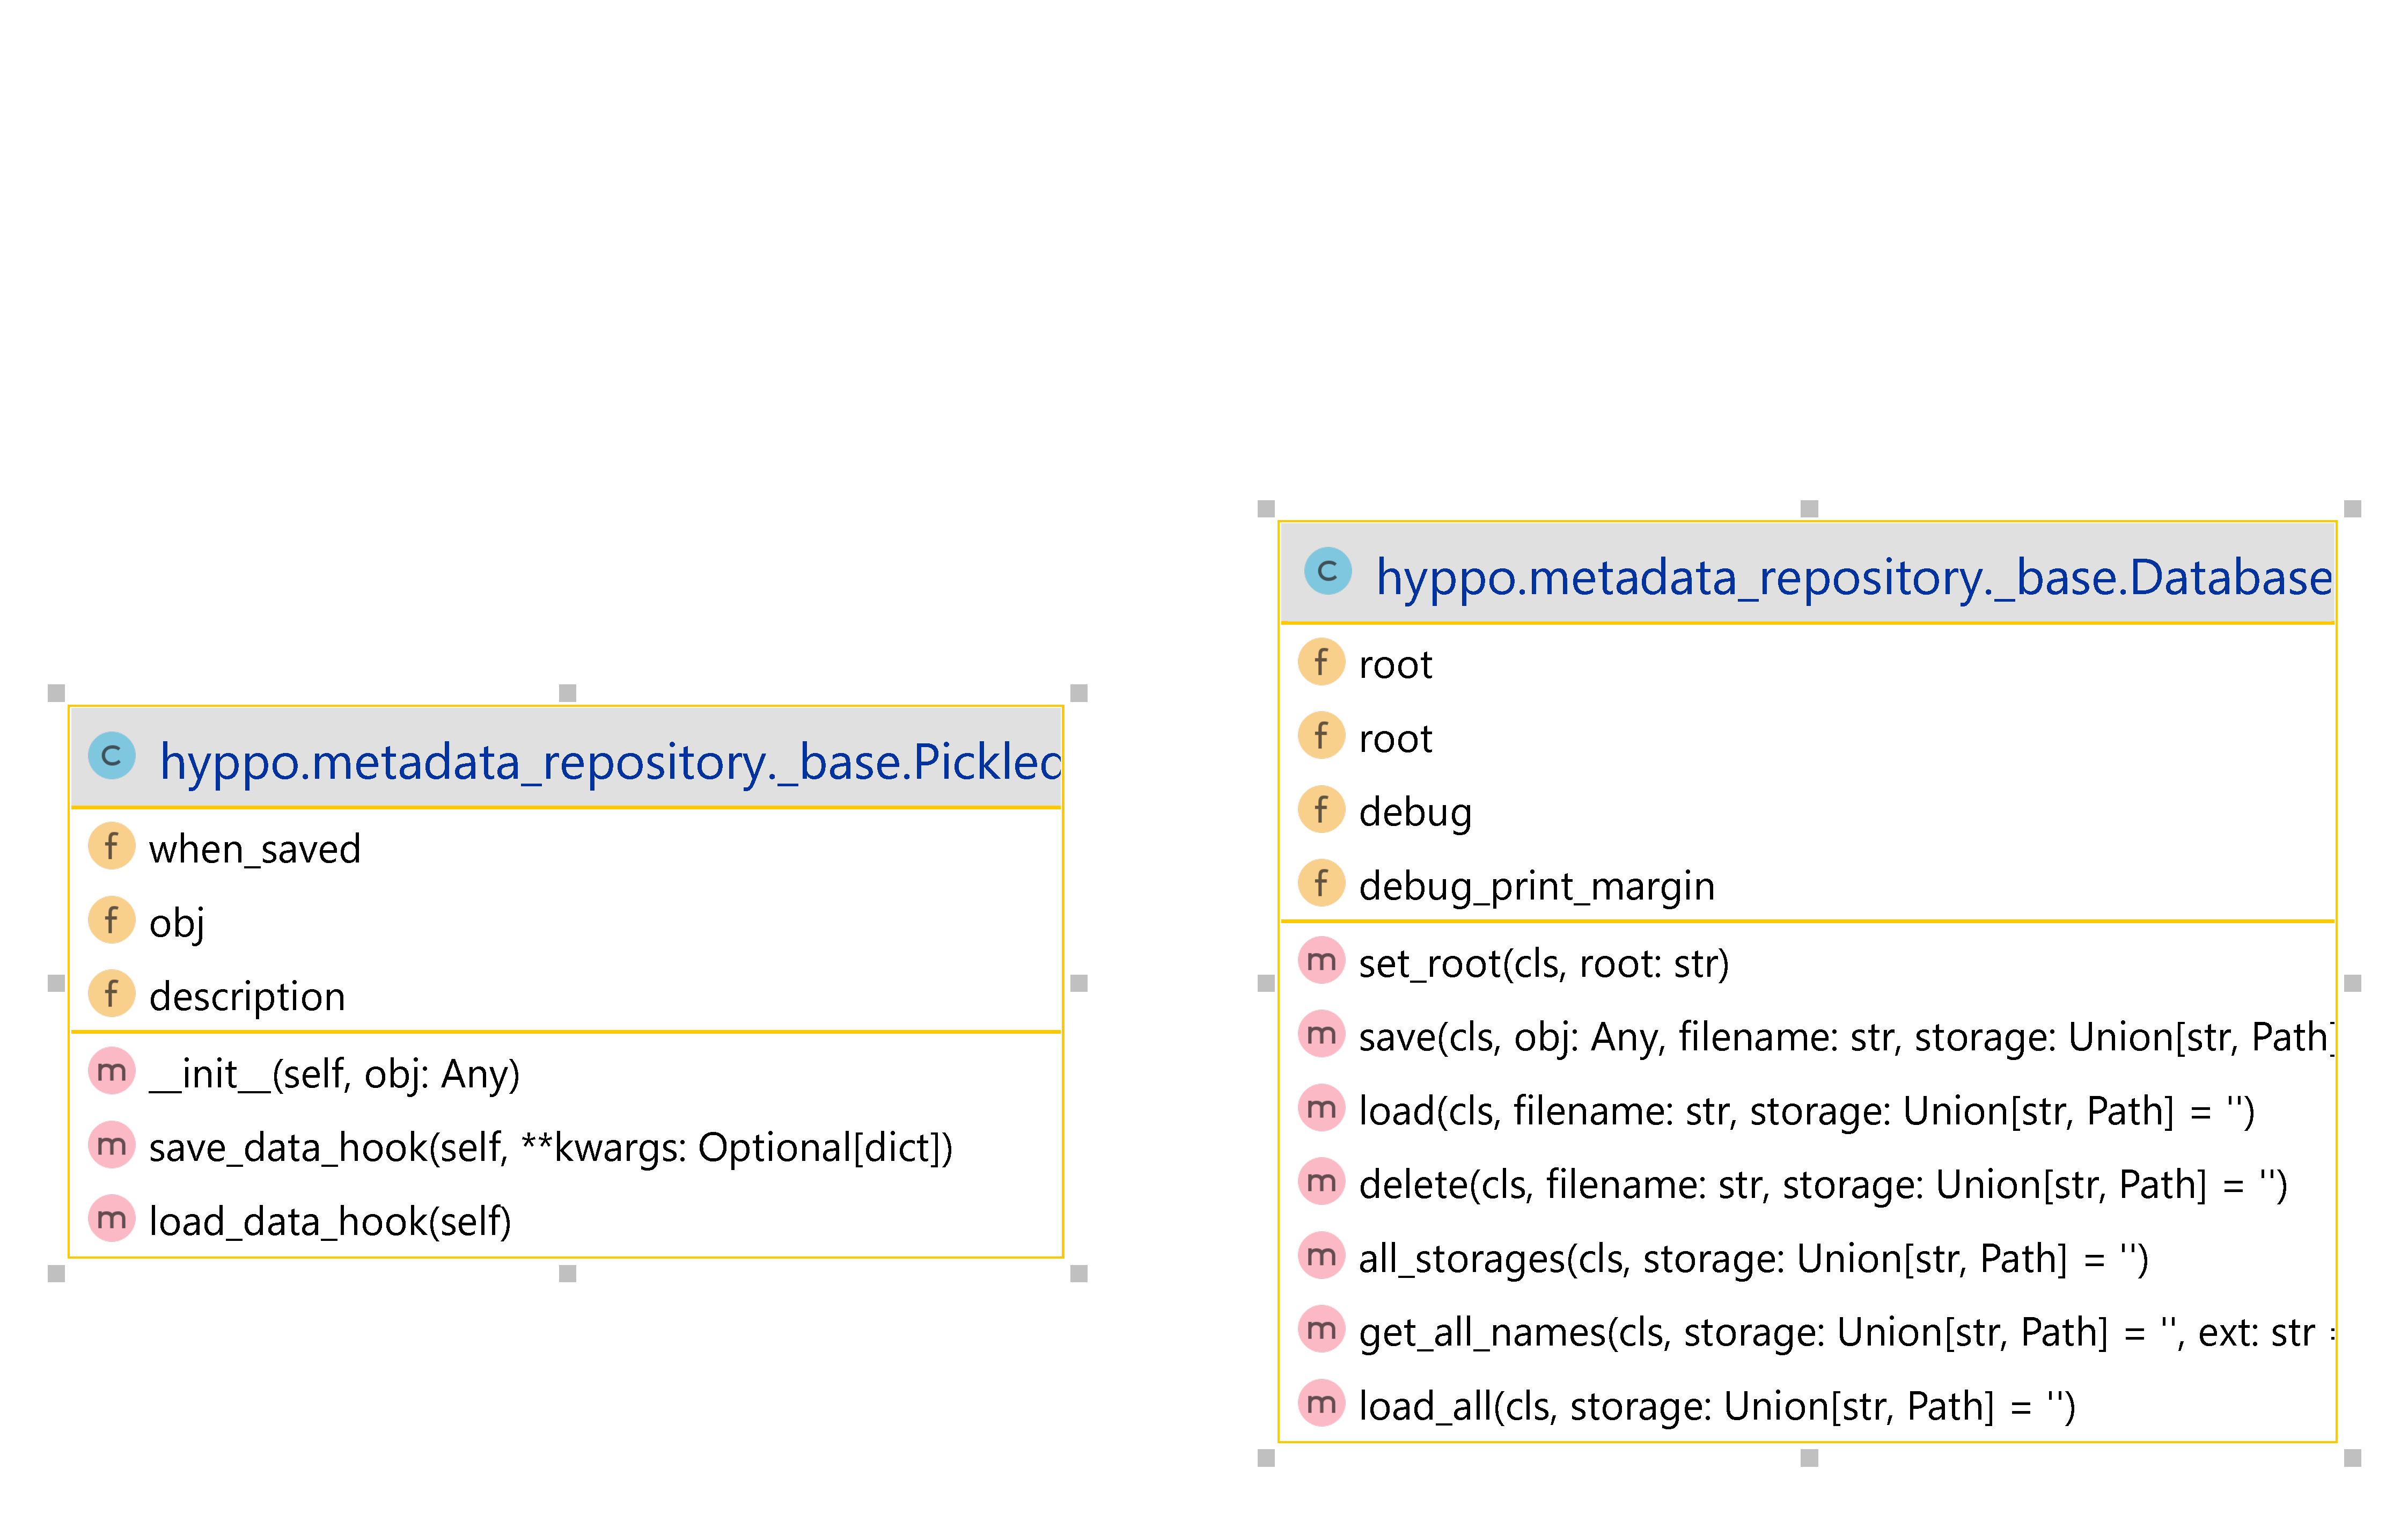
\includegraphics[width=0.9\linewidth]{images/_repo.pdf}
    \caption{Диаграмма для пакета.}\label{fig:repo}
\end{figure}
\cref{fig:repo}

%\section{Поиск оптимальных параметров гипотез}\label{sect_4_5}
\section{Инфраструктура для работы с платформой}\label{sect_4_5}

\subsection{Аппаратное и программное обеспечение кластера}\label{sect_4_5_1}

Эксперименты по адаптации программной реализации нейросетевых моделей для выполнения в распределенной 
вычислительной среде были проведены с использованием прототипа вычислительного кластера. Кластер включает в 
себя главный узел и четыре вычислительных узла и развернут как часть инфраструктуры совместных исследовательских 
объектов для высокопроизводительных вычислений ФИЦ ИУ РАН. Аппаратная архитектура кластера показана на 
\cref{fig:lab_cluster}. Вычислительные узлы включают в себя два процессора Intel Xeon 2630L с частотой 2,5 ГГц и 
24 виртуальными ядрами, 64 ГБ оперативной памяти DDR3 1066 МГц, один твердотельный накопитель емкостью 160 Гб и 
четыре жестких диска емкостью 2 ТБ каждый. Кластер также включает файловый сервер Quanta Stratos S810 с двумя 
процессорами Intel XEON 2670, 96 ГБ оперативной памяти DDR3 1066 МГц, один твердотельный накопитель INTEL S3500 
емкостью 480 ГБ, RAID-массив, состоящий из 15 жестких дисков по 2 ТБ каждый, и RAID-массив, состоящий из 
8 твердотельных накопителей INTEL S3500 емкостью 480 ГБ каждый. Сеть Ethernet поддерживается коммутатором 
Quanta LB6M 10GbE.

\begin{figure}[h!]
    \centering
    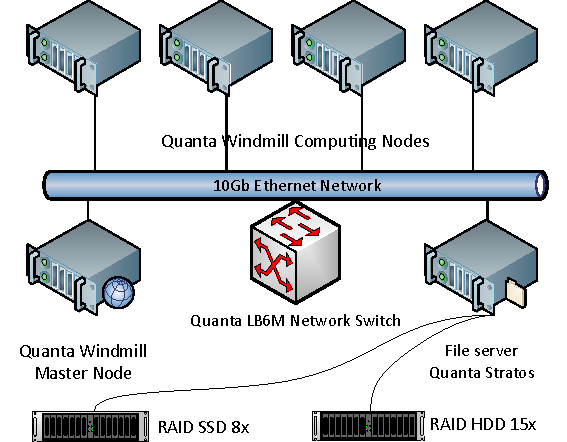
\includegraphics[width=0.7\linewidth]{images/lab_cluster.pdf}
    \caption{Инфраструктура платформы исполнения виртуальных экспериментов.}\label{fig:lab_cluster}
\end{figure}

На кластере установлена платформа данных Hortonworks с открытым исходным кодом 3.1.4.0 \cite{HDP2021}, 
предназначенная для распределенных вычислений. Платформа основана на платформе распределенного управления 
данными Hadoop \cite{hadoop} и файловой системе HDFS \cite{borthakur2007hadoop}. В частности, платформа включает 
в себя систему управления ресурсами YARN и планирования/мониторинга заданий, а также систему обработки данных Spark, 
предназначенную для распределенного использования общей памяти. 

Распределенная файловая система HDFS устанавливается поверх файловой системы Linux ext3. Файлы хранятся в HDFS в 
виде наборов блоков определенного размера. Разные блоки одного и того же файла могут храниться на разных узлах 
кластера. Блоки файлов реплицируются для обеспечения отказоустойчивости. Несколько реплик блока хранятся на разных 
узлах кластера. Репликация блоков "--- это автоматическая процедура: если файловый блок поврежден, автоматически 
используется реплика. HDFS масштабируется по объему данных: новые узлы могут добавляться в кластер динамически. 

YARN разделяет управление ресурсами и планирование заданий/мониторинг на отдельные демоны: global ResourceManager и 
ApplicationMaster. Экземпляр ApplicationMaster создается для каждого приложения. ResourceManager и NodeManager 
формируют структуру вычислений данных. ResourceManager управляет ресурсами между всеми приложениями в системе. 
Для каждого приложения выделяется контейнер, а также права на использование заданного объема ресурсов (процессор, 
память, диск, сеть). NodeManager - это агент узла для каждого кластера, отвечающий за контейнеры, отслеживающий 
использование их ресурсов и сообщающий об этом ResourceManager. ApplicationMaster согласовывает ресурсы с 
ResourceManager и работает с NodeManager для выполнения и мониторинга задач.

YARN позволяет развертывать различные фреймворки для распределенной обработки данных в кластере Hadoop, такие как 
MapReduce для пакетной обработки, Tez для моделирования обработки данных в виде графика потока данных, Storm 
для потоковой обработки и так далее. 

Spark \cite{zaharia2010spark} - одна из самых популярных систем обработки данных для Hadoop. Spark предназначен 
для хранения и обработки данных в распределенной общей памяти, повышающей производительность при решении различного 
рода задач. Spark особенно полезен для распределенного машинного обучения с итеративными алгоритмами, посещающими 
наборы данных несколько раз в цикле. Архитектурной особенностью Spark является устойчивый распределенный набор 
данных (RDD), доступный только для чтения мультинабор элементов данных, распределенных по кластеру машин, 
который поддерживается отказоустойчивым способом. RDDS можно манипулировать с помощью различных параллельных операций.

Приложения Spark, называемые драйверами, выполняются как независимые наборы процессов в кластере, координируемые 
объектом SparkContext. SparkContext может подключаться к нескольким типам менеджеров кластеров (например, YARN), 
которые распределяют ресурсы между приложениями. После установления соединения Spark получает исполнителей на 
рабочих узлах кластера, которые представляют собой процессы, выполняющие вычисления и хранящие данные для 
приложения. Код приложения, определенный файлами JAR или Python, передается в SparkContext. Наконец, 
SparkContext отправляет задачи исполнителям для выполнения.

Прототип кластерного программного обеспечения ориентирован на развертывание на платформах облачных вычислений. 
Все программные компоненты инкапсулированы в контейнеры системы виртуализации уровня ОС с открытым 
исходным кодом Docker \cite{anderson2015docker}.

\subsection{Базовое программное обеспечение для запуска платформы на кластере}

Взаимодействие платформы и кластера приведено на \cref{fig:platform_cluster}.

\begin{figure}[h!]
    \centering
    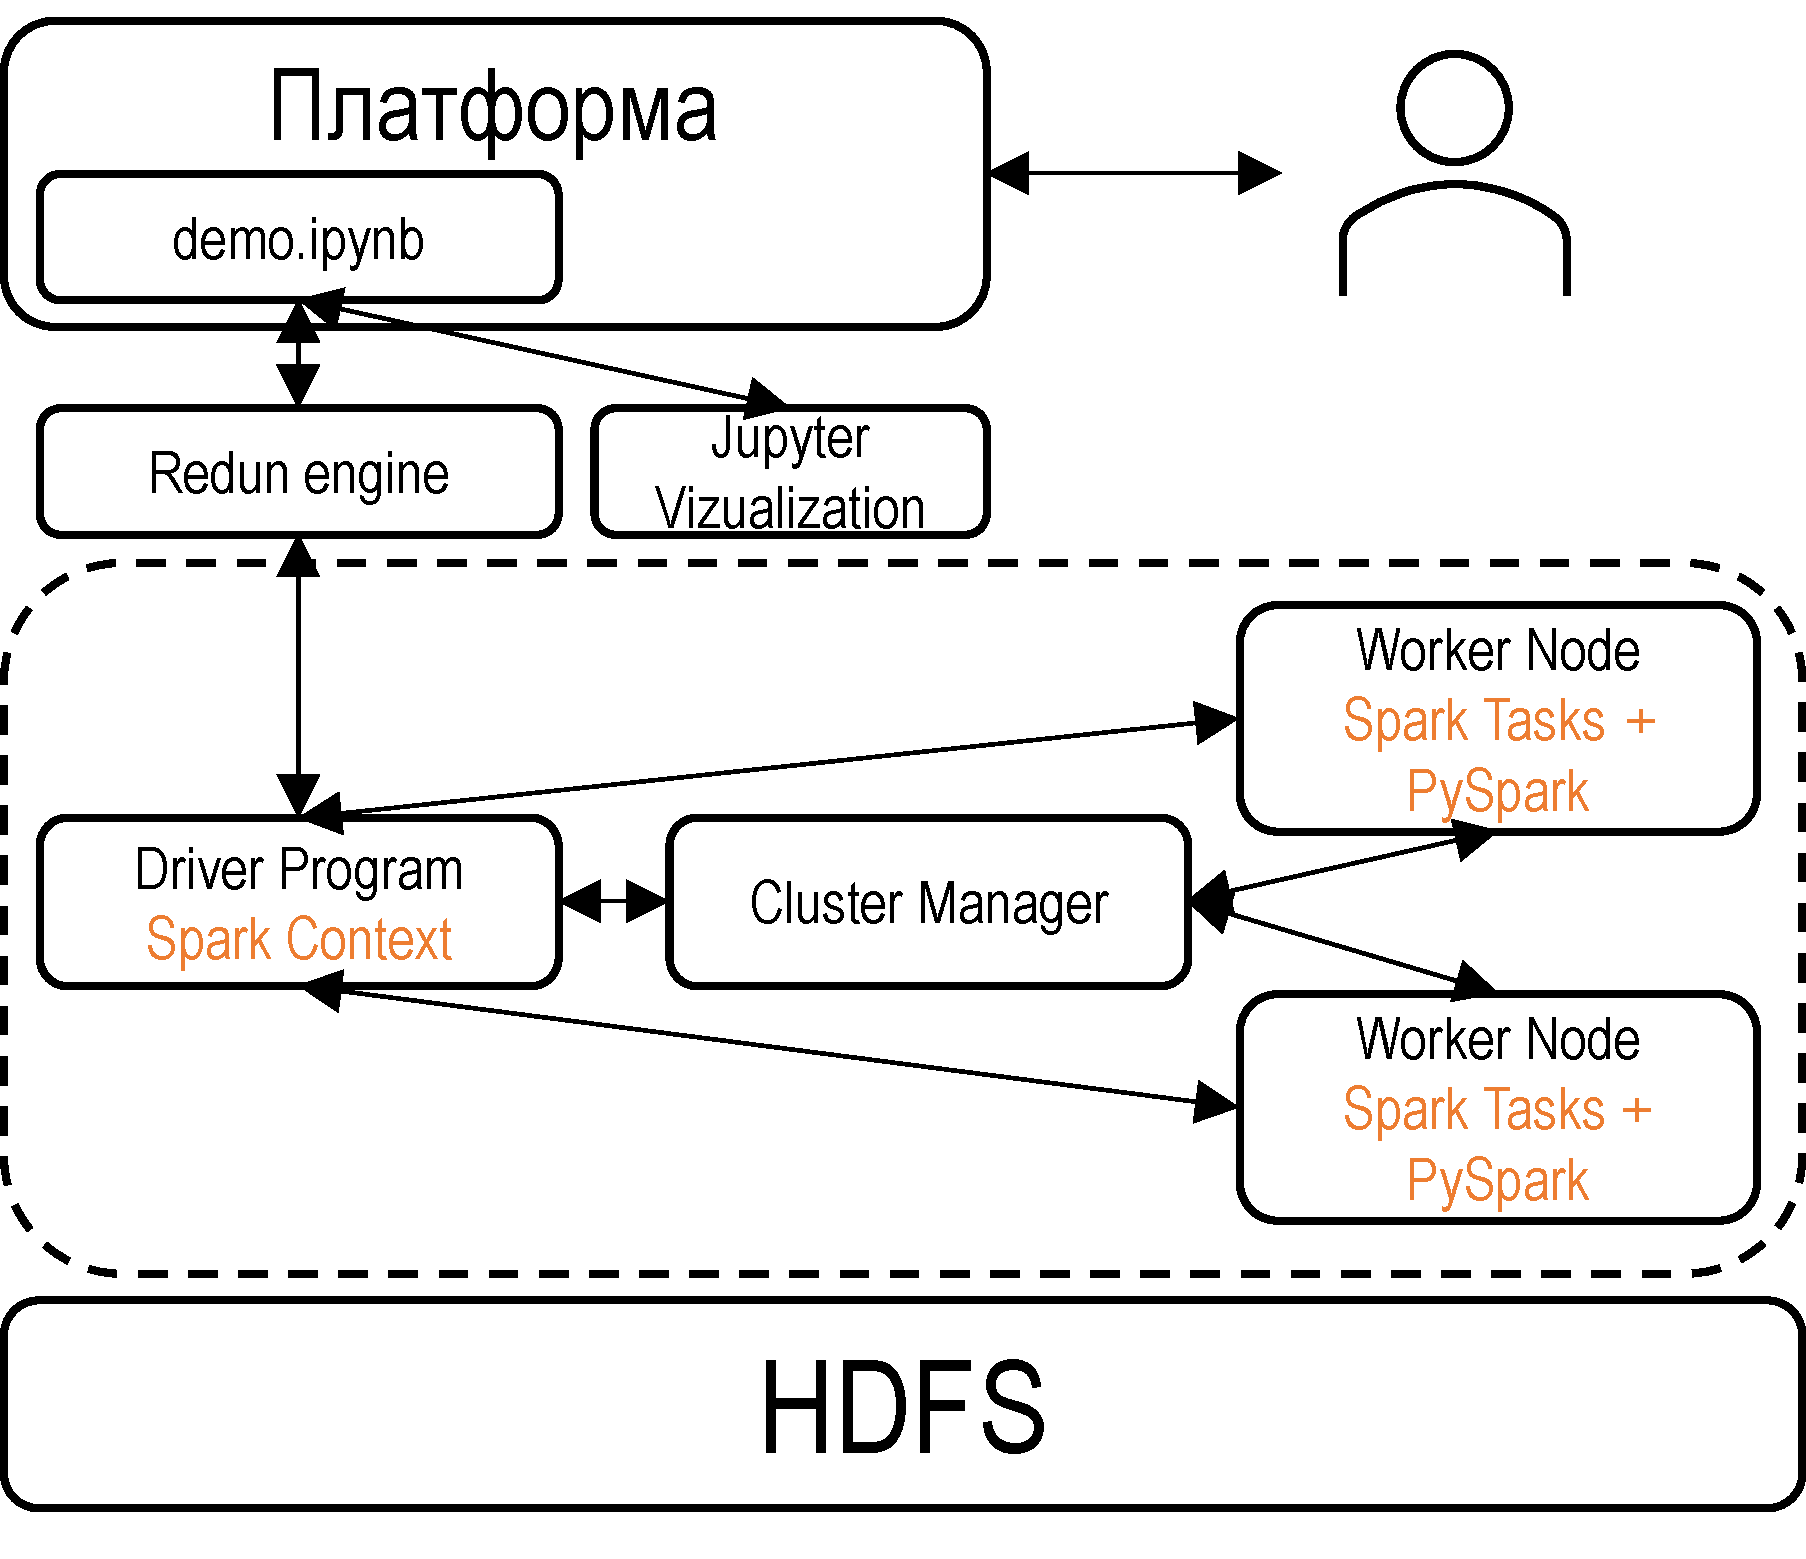
\includegraphics[width=0.7\linewidth]{images/platform_cluster.pdf}
    \caption{Запуск примера с использованием Платформы на кластере.}\label{fig:platform_cluster}
\end{figure}


Nibabel \cite{gorgolewski2011nipype} "--- это библиотека, предоставляющая API для чтения и записи 
некоторых распространенных форматов файлов для нейровизуализации. Эти форматы включают: ANALYZE (обычный, 
SPM99, SPM2 и выше), FIFTY, Nifty 1, Nifty 2, MINS1, MINS2, MGH и EAT, а также Philips PAR/REC. Различные 
классы форматов изображений обеспечивают полный или выборочный доступ к информации заголовка (meta), а 
доступ к данным изображения предоставляется через массивы библиотеки numpy.

Объекты изображения Nibabel состоят из трех элементов:
\begin{enumerate}
    \item $n$-мерный массив, содержащий изображение.
    \item Матрица аффинных преобразований размером 4х4, которая соотносит координаты изображения 
            со стандартным мировым координатным пространством.
    \item Метаданные изображения, хранящиеся в заголовке.
\end{enumerate}

При загрузке изображения создается объект типа Nifti1image. Имя файла может иметь расширение  .nii или .nii.gz. 

Стоит отметить, что при непосредственном вызове функции загрузки данные изображения не загружаются в память, 
поскольку изображения могут храниться в виде массива numpy на диске. Чтобы загрузить данные с диска,  необходимо 
вызвать функцию $get\_data()$ объекта типа Nifti1Image. Эта функция возвращает $n$-мерный массив numpy. Кроме того, 
объект типа Nifti1Image создается из массивов numpy. Чтобы сделать это, необходимо передать $n$-мерный массив данных 
и матрицу аффинного преобразования конструктору Nifti1Image.

Nitime \cite{rokem2009nitime} "--- это библиотека для анализа временных рядов в области нейровизуализации. 
Nitime может использоваться для представления, обработки и анализа данных временных рядов на основе экспериментальных 
данных. Основная цель библиотеки - служить платформой для анализа данных, собранных в ходе нейрофизических 
экспериментов. Основным принципом реализации nitime является разделение представления временных рядов и 
анализа временных рядов.

Важной особенностью библиотеки anytime является отложенная инициализация. Большинство атрибутов как временных 
рядов, так и объектов анализа используются только при необходимости. То есть инициализация объекта временного 
ряда или объекта анализа не вызывает каких-либо интенсивных вычислений. Кроме того, после запуска вычисления 
объект сохраняется и гарантирует, что доступ к результатам анализа приведет к выполнению вычисления только при 
первом выполнении анализа. После этого результат анализа сохраняется для дальнейшего использования. Одним из 
алгоритмов библиотеки nitime является корреляционный анализ областей мозга. Он вычисляет корреляцию между одним 
временным рядом, представляющим данную область мозга, и другими областями, которые также представлены временным 
рядом. Для вычисления корреляции между регионами в библиотеке nitime существует функция SeedCoherencAnalyzer, 
которая принимает два входных данных временных рядов и возвращает корреляционную матрицу, которую можно 
использовать для дальнейшего анализа.

Nilearn \cite{abraham2014machine} "--- это модуль Python для статистической обработки данных нейровизуализации.
Он использует модуль scikit-learn для многомерной статистики с приложениями для интеллектуального моделирования, 
классификации, декодирования и анализа связности. Nilearn может работать с объектами NiftiImage из библиотеки nibabel.
Библиотека Nilearn обладает большой функциональностью для работы с nii-изображениями. Это позволяет визуализировать, 
декодировать, исследовать функциональную связность и выполнять различные манипуляции, такие как сглаживание, 
маркировка и расширенный статистический анализ.
Nilearn предоставляет метод CanICA, который является методом ICA для анализа данных МРТ на групповом уровне. 
По сравнению с другими стратегиями, это обеспечивает хорошо контролируемую групповую модель, а также пороговый 
алгоритм, который контролирует специфичность и чувствительность с помощью явной модели сигнала. 
Чтобы получить временной ряд и построить для него корреляционную матрицу, nilearn предоставляет объект NiftiMapsMasker. 
Чтобы создать объект, нужно указать атлас областей мозга. Nilearn предоставляет возможность создавать корреляционную 
матрицу для независимых компонентов, которая вычисляется CanICA.

Программа считывает все файлы из каталога, проверяет правильность формата (все данные сжаты). После этого номер темы 
извлекается из имени файла и его пол проверяется с помощью дополнительного файла метаданных. Когда пол известен, файл 
распаковывается в соответствующую папку. Внутри распакованной папки находится 4-D изображение в .nii.gz формат. 
Используя библиотеку nibabel, изображение загружается в память в виде массива типа numpy.array. Из этого массива 
создается новый массив с информацией о пространственных координатах перед значением вокселя. Новый массив с
жимается с помощью алгоритма gzip и сохраняется в HDFS.

Задачи Spark запускаются со следующими параметрами:
\begin{itemize}
    \item \textit{num-исполнитель = 4} - количество исполняемых объектов.
    \item \textit{executor-memory = 25GB} - объем памяти, используемый для одного процесса выполнения.
    \item \textit{executor-cores = 2} - количество ядер, используемых для каждого исполнительного объекта.
    \item \textit{driver-memory = 8GB} - объем памяти, используемый для процесса драйвера.
\end{itemize}

\section{Выводы по главе}\label{sect3_3}
\clearpage
           % Глава 3
\chapter{Методика организации виртуальных экспериментов в практических задачах} \label{chapt3}

\section{Задачи по анализу сигналов фМРТ в нейрофизиологии}\label{sect_4_1}
\subsection{Введение}
Для сообщества, занимающегося нейронаукой, разработка общих парадигм исследования огромного числа функциональных систем 
в головном мозге все еще остается труднейшей задачей. Построенный на термине коннектом, изобретенном для описания 
подробной карты соединений нейронов в мозге человека, термин функциональный коннектом обозначает совокупное множество 
функциональных соединений в мозге (его схему коммутации) \cite{biswal2010toward}. В более широком смысле коннектом 
включает в себя отображение всех нейронных соединений нервной системы организма. Вопросы образования и изучения 
коннектома, известные как коннектомика, могут простираться по своему масштабу от детальной карты полного набора 
нейронов и синапсов в пределах части или всей нервной системы организма до описания макромасштабных процессов 
\cite{craddock2013imaging} функциональной и структурной межнейронной коннективности между всеми полями коры головного 
мозга и субкортикальными структурами. Конечная цель коннектомики "--- картирование мозга человека. В функциональной 
магниторезонансной томографии (fMRI "--- фМРТ) считается, что визуализируемые соединения представляют собой 
функциональную связность в том смысле, что две области мозга совместно участвуют в реализации некоторой более высокого 
порядка функции, нередко в контексте выполнения определенной задачи. 

Технология fMRI стала мощным инструментом, используемым для изучения многочисленных функциональных схем одновременно. 
Это привлекло к себе внимание статистиков, работающих в этой сфере. На уровне элементарных измерений данные 
нейровизуализации могут, в основном, рассматриваться как состоящие из ряда сигналов (как правило, последовательных во 
времени) в каждой совокупности пикселей (в двух измерениях) или вокселей (в трех измерениях). Исходя из этих данных, 
нейровизуализация использует различные формы представления информации более высокого уровня. За последние годы в 
нейровизуализации возник существенный интерес к представлениям на основе сетей, где сети (графы) используются для 
обобщения информации о связях в множестве измерений, обычно предполагающих отражение функциональных или структурных 
отношений между исследуемыми областями мозга. Нетрудно предсказать, что поскольку нейровизуализация стала теперь 
стандартным инструментом клинической нейронауки, мы быстро движемся к моменту, когда в нашем распоряжении окажутся 
доступные базы данных, состоящие из больших массивов вторичной информации в виде объектов данных на основе сетей. 

Одной из наиболее фундаментальных задач, представляющих интерес в анализе таких данных, является проверка гипотез, 
отвечающих на такие вопросы, как Есть ли разница между сетями (графами) этих двух групп объектов?. Сети не являются 
эвклидовыми объектами, и поэтому классические методы статистики здесь нельзя применять непосредственно. Аналоги 
классических инструментов оценки (на основе статистики) и проверки гипотез исследуются в 
\cite{ginestet2017hypothesis, ginestet2014statistical}. Такое исследование мотивировано проектом 1000 функциональных 
коннектомов (1000 FCP), запущенном в 2010 г. \cite{biswal2010toward}. Проект 1000 FCP \cite{yan2013standardizing} 
включает в себя самое большое множество данных такого рода, сходного с большими множествами данных в генетике. 
В проект 1000 FCP включено описание данных функциональной нейровизуализации 1093-х субъектов, находящихся в 
24 центрах сообщества. Средний возраст участников "--- 29 лет, а все субъекты были возрастом 18 лет или старше.


Другие проекты (такие как проект Коннектом человека (Human Connectome Project "--- HCP) \cite{VanEssen2013}) имеют 
целью построить сетевую карту (граф) мозга здорового, живого взрослого человека. Суммарный объем данных, выдаваемых 
проектом HCP, будет, по-видимому, составлять много петабайтов \cite{VanEssen2013}. Из информатики платформа HCP 
включает в себя как платформу систему управления данными ConnectomeDB на базе платформы визуализации XNAT из той 
же информатики \cite{marcus2007extensible}, широко используемую систему с открытым кодом для управления и совместного 
пользования данными визуализации и взаимосвязанными данными. В настоящее время проект HCP располагает информацией о 
более чем 1000 субъектам, включая структурные сканы (\textit{T1w} и \textit{T2w}), fMRI в покое (rfMRI), 
fMRI действия (tfMRI) при выполнении задачи, а также диффузионная визуализация МРТ (dMRI) с высокой угловой 
разрешающей способностью. Кроме того, доступны данные MEG в покое (rMEG) и/или данные MEG (tMEG) при выполнении задачи. 
Данные поступают в нескольких форматах: необработанные сырые данные, предварительно минимально обработанные, 
а также наборы данных по результатам анализа. В предварительно обработанных наборах данных пространственные нарушения 
минимальны, а данные были выровнены по их модальностям и по субъектам с использованием соответствующих методов 
регистрации по объемам и по поверхностям. Сообщество исполнителей проекта HCP рекомендует пользоваться 
предобработанными наборами данных. 

Можно ожидать, что в ближайшем будущем в нейронауке появится большое количество баз данных сетевых объектов, 
мотивирующих разработку и расширение различных инструментов от классической статистики до глобальных сетевых данных.

Исследование функциональной связности с помощью fMRI широко используется, так как метод обладает высоким 
пространственным разрешением, анализ проводится интактно, не требуя инъекций или хирургических вмешательств. 
Данные fMRI представляют собой 4-х мерные изображения (одна временная координата и три пространственных) и 
предназначены для регистрации гемодинамических реакций головного мозга, вызванных активностью нейронов. 
Различают два типа fMRI: 1) изображения fMRI, которые были получены, когда человек находился в состоянии 
покоя, то есть во время проведения эксперимента испытуемого просили закрыть глаза, расслабиться и ни о чем не 
думать; 2) изображения fMRI, которые были получены во время некоторого действия, например, у испытуемого 
стимулируется проявление эмоций, зрительных или двигательных реакций и пр. Изображения fMRI имеют сложную 
структуру и требуют больших ресурсов для их хранения, таких как высокопроизводительные вычислительные системы. 

% TODO типы взаимодействия
%Существует три типа взаимодействия между регионами головного мозга: структурное, эффективное и функциональное. 
Исследование функциональной связности в состоянии покоя имеет существенное значение, так как полученные результаты 
позволяют выделять нейросети покоя и анализировать их активность. Другим примером связности является эффективная 
связность. Анализ эффективной связности показателей fMRI действия позволяют оценить участие конкретных структур 
мозга в обеспечении сложных функций, таких как язык, память, азартная игра, движения. Эти подходы используются для 
изучения когнитивных и других функций мозга, а также для исследования различных заболеваний: болезни Паркинсона, 
синдром дефицита внимания/гиперактивности, болезни Альцгеймера и др. Задачи исследования различных типов связности 
являются актуальными и представляют существенный интерес.

\subsection{Выделение регионов головного мозга из fMRI изображений}

Визуализация, обработка и анализ многомерных данных, таких как изображения, часто требует некоторой предварительной 
обработки, для того чтобы уменьшить размерность данных и получить отображение исходно представленных данных на 
низкоразмерное векторное пространство. Предположение таково, что исходные данные находятся в низкоразмерном 
подпространстве или многообразии \cite{brun2006manifold}, вложенном в исходное пространство. Эта часть исследований 
называется сокращением размерности, или нелинейным сокращением размерности, включающей в себя методы параметризации 
данных с использованием низкоразмерных многообразий (манифольдов) в качестве моделей. В сообществе обработчиков 
информации по нейронам это известно под названием обучения на базе многообразий. Методы обучения на базе многообразий 
дают возможность отыскивать нелинейные параметризации многообразий информационных точек, находящихся в высокоразмерных 
пространствах, весьма сходно с тем, как метод главных компонент (МГК) способен узнавать или выявлять наиболее важное 
линейное подпространство набора информационных точек (проецируя данные на $n$-размерное линейное подпространство, 
которое дает максимум дисперсии распределения вероятностей данных в новом пространстве). Такие преобразования 
называются выделением регионов головного мозга человека.

В качестве переменных для построения зависимостей используются регионы головного мозга (ROI). ROI "--- это набор 
анатомически близких вокселей, которые представляют собой встроенные единицы изображения МРТ, представляющие маленькие 
кубики мозга. Поскольку изображение МРТ фиксирует изменения во времени уровня кислорода в крови, каждый воксель связан 
с соответствующим временным рядом. ROI также связаны с временными рядами, например, усредненными по всем временным 
рядам его вокселей. На данном этапе требуется преобразовать 4-х мерное изображение головного мозга в двухмерный массив 
(регионы головного мозга "--- время). Выделение регионов можно рассматривать как один из способов уменьшения размерности. 
При использовании данного подхода регионы некоторым образом группируются и усредняются, а само усредненное значение 
является представительным значением для данного региона. Также при использовании данного метода делается предположение, 
что воксели одного региона ведут себя схожим образом. 

Существует множество методов для выделения регионов головного мозга \cite{Arslan2018}. Все методы можно разделить 
на три группы:
\begin{enumerate}
    \item Выделение регионов для одного человека (субъекта);
    \item Выделение для группы людей;
    \item Использование различных атласов головного мозга человека.
\end{enumerate}

Методы первого типа подразделяют поверхность головного мозга каждого субъекта независимо друг от друга. Часть методов 
в данном подходе основа-на на широко используемых алгоритмах кластеризации, таких как $k$-средних 
\cite{arslan2015multi}, агломеративной иерархической кластеризации \cite{blumensath2013spatially} и 
спектральной кластеризации \cite{van2008normalized}. Если набор данных состоит из нескольких субъектов, 
то первоначально все данные объединяются в один большой набор, состоящий из $M$ субъектов, а затем применяются МГК/МНК.

При больших наборах данных или при большом количестве субъектов становится неразумным формировать полный набор 
данных, а затем применять МГК и МНК из-за ограничений по памяти и по вычислительному времени. Для решения этой 
проблемы было предложено использовать групповые методы. Групповые методы строят репрезентативные модели популяции. 
Методы получения регионов группового уровня обычно основываются на предположении, что пространственное соответствие 
между субъектами было обеспечено априори. Следовательно, каждая вершина (или воксель) представляет собой одно и 
то же пространственное положение для каждого субъекта. Это позволяет объединить или усреднить данные по различным 
субъектам для анализа на популяционном уровне. Существует два наиболее популярных способа.

Первым способом является вычисление регионов для каждого субъекта индивидуально, а затем применение второго уровня 
алгоритма кластеризации на уровне популяции (т. е. двухуровневый подход). Двухуровневый подход обеспечивает 
группировку вокселей одних и тех же регионов вместе. В результате регионы группового уровня, полученные с помощью 
этого метода, выражают общие характеристики популяции, аппроксимируемые регионами, полученные для каждого субъекта 
в отдельности. Примером является применение двухуровненого применение метода главных компонент 
\cite{calhoun2001method} (см. \cref{fig:two_step_pca}). Сначала каждый набор данных сокращается до $\rho$ основных 
пространственных векторов с использованием МГК, а затем объединив их и применив еще раз  МГК, чтобы уменьшить 
конечный набор данных до $k$ компонент.

\begin{figure}[ht]
    \centering
    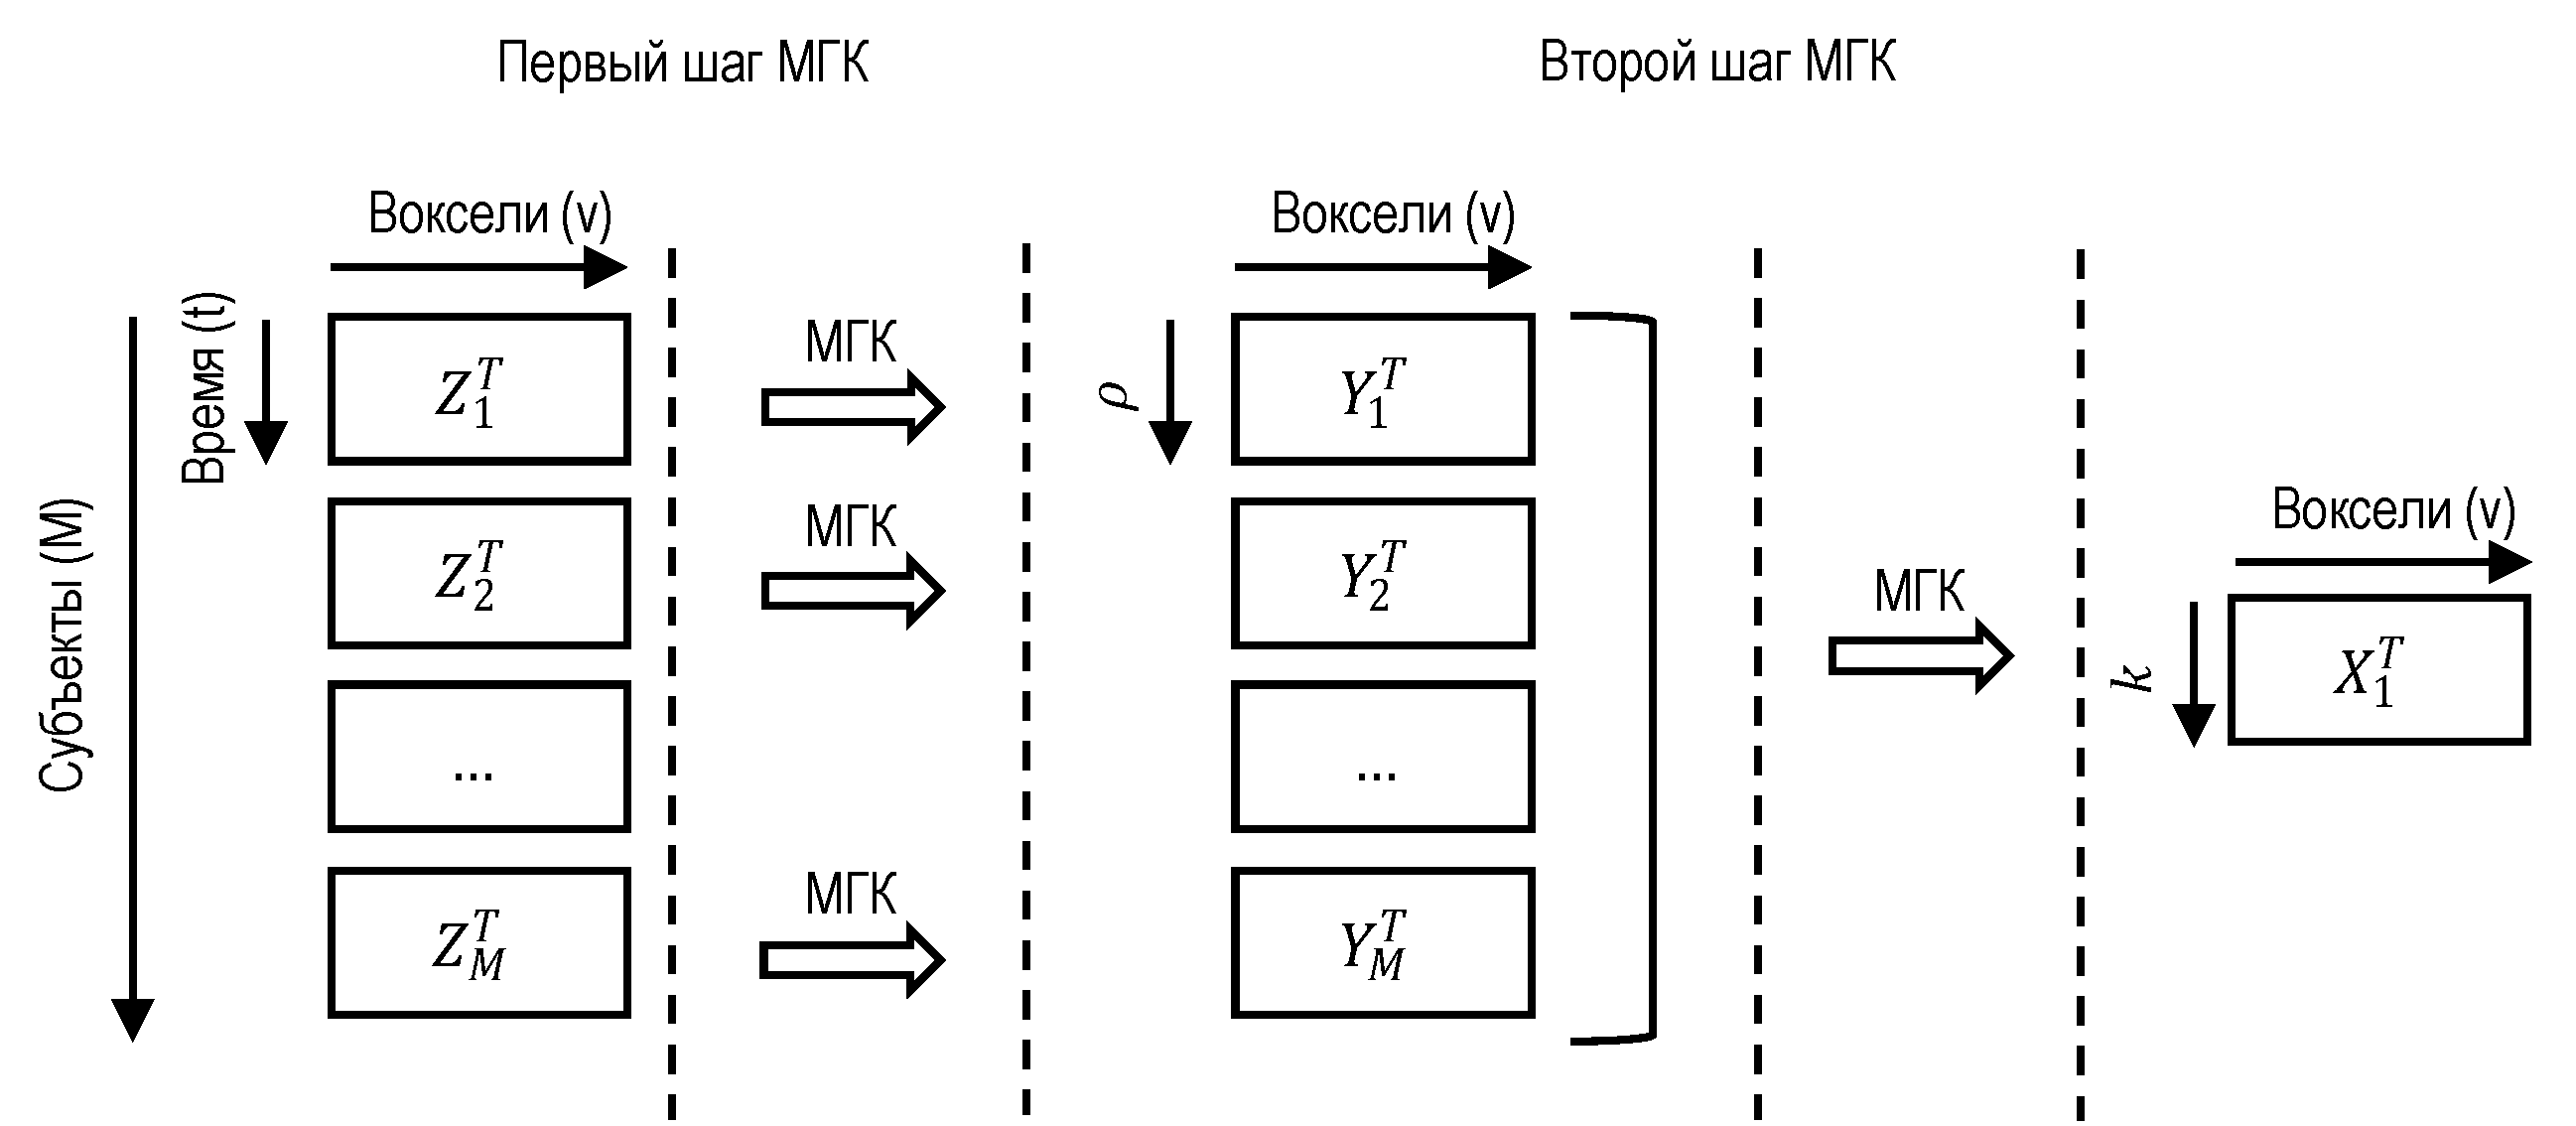
\includegraphics[width=1.0\linewidth]{images/two_step_pca.pdf}
    \caption{Двухуровненое применение метода главных компонент.}\label{fig:two_step_pca}
\end{figure}

Хотя использование небольшого значения $m$ ограничивает требования к памяти для этих операций, размер данных 
масштабируется линейно с количеством объектов, которые в конечном итоге могут стать непрактично большими. 
Кроме того, важная часть информации может быть потеряна, если $m$ не является относительно большим (обычно оно 
не должно быть большим). Информацию может быть трудно оценить на уровне отдельного субъекта, но она может быть 
важна на уровне группы. 

Вторым способом является вычисление репрезентативной матрицы признаков из популяции, например, путем объединения 
временных рядов и далее подходу группового среднего. Данный метод направлен на поиск общих паттернов между 
индивидами в пределах популяции путем вычисления группового среднего представления, что достигается путем объединения 
временных рядов каждого субъекта и применения метода главных компонент или его модификаций для уменьшения 
размерности для выделения регионов (см. \cref{fig:group_pca}). Широко используемым является алгоритм MELODIC 
Incremental Group-PCA (MIGP) \cite{rachakonda2016memory} . MIGP "--- это инкрементный подход, целью которого 
является обеспечение очень близкого приближения к полной конкатенации набора данных, за которым следует МГК, 
но без больших требований к памяти. Высокая точность достигается за счет того, что отдельные наборы данных 
субъектов не сводятся к небольшому числу компонентов МГК. Инкрементный подход сохраняет внутреннее пространство 
МГК из $m$ взвешенных пространственных собственных векторов, где $m$ обычно больше, чем количество временных 
точек в каждом отдельном наборе данных. Под "взвешенным" подразумевается, что собственные значения включены в 
матрицу пространственных собственных векторов. Конечный набор из $m$ компонентов, представляющих временно 
объединенные выходные данные МГК, затем может быть уменьшен до требуемого размера $n$ просто путем сохранения 
верхних $n$ компонентов и, при необходимости, отбрасывания весовых коэффициентов (собственных значений).

Обычно сначала объединяются 2-3 субъекта. Затем этот набор данных вводится в $m$-мерный объект и получается 
следующая матрица. Каждый вектор умножается на свое собственное значение. Собственные значения характеризуют 
важность компонента здесь, поэтому статистическая информация не теряется и сохраняется дисперсия каждого субъекта. 
MIGP не увеличивает требования к памяти с увеличением числа объектов, большие матрицы никогда не формируются, 
а время вычисления линейно зависит от количества объектов.

\begin{figure}[ht]
    \centering
    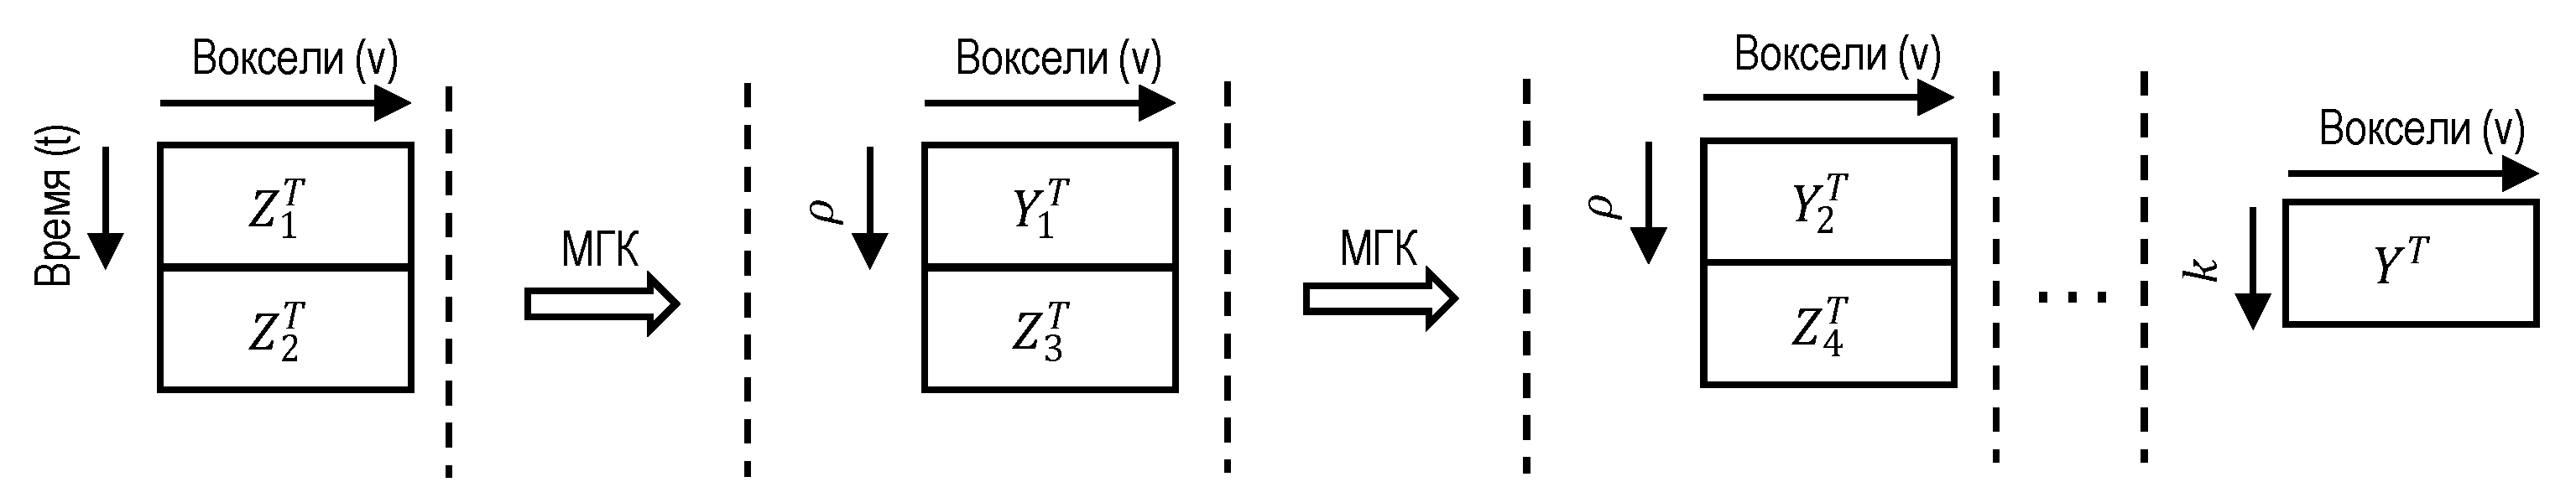
\includegraphics[width=1.0\linewidth]{images/group_pca.pdf}
    \caption{Последовательное применение метода главных компонент.}\label{fig:group_pca}
\end{figure}

При работе с атласами головного мозга человека используется заранее вычисленная функция, ставящая каждому вокселю 
изображения в соответствие регион головного мозга. Существует множество атласов головного мозга человека, например, 
вероятностный атлас Harvard-oxford \cite{desikan2006automated}, в котором описано 48 кортикальных регионов и 
23 субкортикальных. В работе \cite{fischl2004automatically} проводились ряд экспериментов по результатам 
которых делается вывод об оптимальном количестве структурных регионов. Проведен сравнительный анализ на 
нескольких наборах данных между ручной разметкой и при помощи атласа Destrieux 2009. Авторы статьи утверждают, 
что оптимальное количество регионов в атласе 150"---160, при таком количестве удаться достичь баланс между 
размерностью данных и качеством извлекаемого сигнала. Automated Anatomical Labeling (AAL) атлас является 
результатом автоматической анатомической маркировки пространственно нормализованного набора данных фМРТ 
высокого разрешения, предоставленного Монреальским неврологическим институтом (MNI). Данный атлас 
включает 116 структурных областей головного мозга \cite{tzourio2002automated}.

 
\subsection{Анализ функциональной связности линейными и нелинейными методами}
Существует два типа функциональной связности головного мозга человека: линейная и нелинейная. В большинстве 
случаев исследуется лишь линейная функциональная связность. Хотя линейная модель проста и полезна в некоторых 
исследованиях \cite{soch2017improve, eklund2017bayesian, kovalev2017search}, однако использование лишь 
линейных функций является сильным ограничением. Так, в работах \cite{lahaye2003functional, karanikolas2016multi} 
показано, что функциональная связность между некоторыми областями мозга является нелинейной, что показывает 
актуальность проблемы исследования нелинейной функциональной связности. Одним из способов изучения нелинейной 
функциональной связности является построение и исследование аналитических функций, как, например, 
в статье \cite{allgaier2015nonlinear}, где авторы строят аналитические функции с помощью генетического 
программирования (ГП) и на основе полученных результатов делают выводы о взаимосвязях тех или иных регионов.


Обобщенная линейная модель является одним из популярных методов изучения нейрофизиологических изображений 
\cite{lahaye2003functional, karanikolas2016multi}. Из всех рассматриваемых методов обобщенная линейная 
модель является наименее трудно вычислимой, а полученный результат достаточно просто интерпретируется. 
При этом для поиска нелинейной функциональной связности метод требует модификации. Между двумя регионами 
головного мозга экспертом определяется некоторая нелинейная функция, которая отображает нелинейное 
взаимодействие между значениями регионов и подается в качестве входного значения для линейной модели. 
Недостатком метода является то, что нужно определять такие нелинейные зависимости заранее.

Для автоматического восстановления нелинейных функциональных связей также используется метод генетического 
программирования. Генетическое программирование не является настолько популярным методом, как обобщенная 
линейная модель, так как этот метод требователен к вычислительным ресурсам. В работе \cite{allgaier2015nonlinear} 
авторы показывают применение данного алгоритма, его преимущества и недостатки. Преимуществом является то, что 
заранее не делается никаких выводов о функциональной связности, как это происходит с обобщенной линейной моделью. 
Существенным недостатком данного алгоритма является то, что его вычислительная сложность растет экспоненциально с 
увеличением размерности входных данных. В \cite{Icke2014} предложен модифицированный метод генетического 
программирования, частично решающий проблему вычислительной сложности. На вход алгоритма подаются функции 
попарного произведения показателей регионов головного мозга, для которых строится обобщенная линейная модель, 
для которой отбираются только значимые пары. Отобранные пары затем используются в качестве входных значений 
для генетического алгоритма. Данный подход демонстрирует лучшие результаты по сравнению с простым алгоритмом 
генетического программирования. Недостатком такого подхода является то, что, что взаимосвязь между некоторыми 
регионами может быть потеряна. Также он, в отличие от нейронных сетей, позволяет в явном виде оценить 
эту связь, так как если даже получится выписать результат для многослойного перцептрона, 
то он будет сложен для понимания.


\subsection{Поиск значимых различий  функциональной связности головного мозга для разных групп людей в состоянии покоя}


Задача поиска различий в работе головного мозга между мужчиной и женщиной уже давно интересует нейрофизиологов. 
В начале 2000-х годов появились работы, где показаны сравнение функционирования головного мозга у мужчин и женщин. 
В статье \cite{koch2007gender} показано, у мужчин и женщин было обнаружено значительное ухудшение показателей 
рабочей памяти в результате возбуждении отрицательных эмоций. Однако фМРТ-анализ выявил отчетливые различия в 
активации нейронов. У мужчин когнитивные показатели при возбуждении отрицательных эмоций были связаны 
с расширенными паттернами активации преимущественно в префронтальной и верхней теменной областях. 
У женщин взаимодействие между эмоциями и рабочей памятью приводило к значительно более сильной реакции 
в миндалевидном теле и орбитофронтальной коре. В статье \cite{xu2015gender} показано, что у мужчин и женщин 
в состоянии покоя есть различия показателей фМРТ в первичной зрительной коре, задней срединной префронтальной 
сети и других отделов головного мозга. Более того, у мужчин и женщин отличается работа головного мозга во время 
болезней. В работе \cite{zang2004regional} изучаются различия фМРТ у мужчин и женщин с рассеянным склерозом. 
Демонстрируется, что при рассеянном склерозе у мужчин проявляется 
более слабая активность в хвостатом ядре по сравнению с женщинами.

Интересно сравнить субъектно-специфичные сети мужчин и женщин в наборе данных 1\'000 FCP. В работе 
\cite{ginestet2017hypothesis} база данных проекта 1000 FCP проводится сравнение сетей, принимая во внимание 
пол субъектов, по разным возрастным группам, а также по разным местам сбора данных. Показано, 
что необходим расчет средних значений по каждой подгруппе сетей. Задача была выполнена путем 
конструирования эвклидовой средней лапласианов для каждой группы субъектов в разных возрастных группах. 
Такие группо-специфичные средние лапласианы могут в дальнейшем интерпретироваться в каждой группе 
как средние функциональные коннективности. Такой подход обеспечивает построение тестов для гипотез 
относительно средних по сетям или группам сетей в целях исследования влияния пола по всем сетям. 
Что касается набора данных 1000 FCP, тестирование с помощью двухвыборочного критерия для лапласианов 
производилась относительно того, существенно ли гендерные различия влияют на характерные особенности 
коннективности мозга. Нулевая гипотеза об отсутствии различий между группами была отброшена. 
Подобным же образом с высокой вероятность была отвергнута нулевая гипотеза по трем возрастным когортам.

В работе \cite{ginestet2017hypothesis} устанавливаются необходимые математические характеристики, связанные 
с определенным понятием пространства сетей, используемых для интерпретации функциональной нейровизуализации 
ориентированных на коннектом данных. Однако расширение инструментов классической статистики на наборы данных 
на сетевой основе оказалось в высокой степени нетривиальным. Основной трудностью такого расширения оказалось 
то, что сети не являются эвклидовыми объектами (для которых классические методы и были разработаны) "--- это, 
скорее, комбинаторные объекты, определенные ими наборами вершин и ребер. В работе \cite{ginestet2017hypothesis} 
показано, что сети могут быть связаны с определенными натуральными подмножествами эвклидова пространства, 
и демонстрируется, что используя сочетание инструментов геометрии, вероятности на многообразиях, а также 
высокоразмерного статистического анализа, можно разработать основанную на принципах и практическую структуру по 
аналогии с классическими инструментами. Так, в частности, была разработана асимптотическая структура для тестирования 
гипотезы, основанной на одной или двух выборках. Ключом к такому подходу является соответствие между 
неориентированным графом и его лапласианом, где последний определен как матрица (связанная с сетью). 
Лапласиан графа оказался наиболее подходящим для использования в таких матрицах. Пространство лапласианов 
графа используется при работе с определенными подмножествами эвклидова пространства, которые являются 
подмногообразиями стандартного эвклидова пространства.


Недостатком рассмотренных выше работ является применение лишь линейных методов для сравнения регионов 
(в основном это обычная корреляция Пирсона). При использовании нелинейной функциональной связности становится 
возможным более подробно исследовать взаимосвязь между регионами головного мозга и лучше понять его работу в целом. 
В будущем это позволит облегчить поставку диагнозов у мужчин и женщин, а также у людей разного возраста, 
и диагностировать заболевания на более ранних стадиях и разработать более эффективное лечение. Исследование 
подходов к поиску значимых различий нелинейной функциональной связности головного мозга для мужчин и женщин 
в состоянии покоя является актуальной задачей, так как позволит выявить различия с помощью нелинейных методов. 
При использовании нелинейной функциональной связности становится возможным более подробно исследовать 
взаимосвязь между регионами головного мозга и лучше понять его работу в целом.

\subsection{Сквозной пример}
В качестве входного набора данных используется 1133 изображения фМРТ покоя проекта HCP. Для каждого человека 
было проведено по четыре эксперимента. Каждый эксперимент длился 14,4 минуты, временной шаг составлял 0,72 секунды. 
фМРТ-изображение — это 4D-изображение (пространственные и временные координаты), которое использует формат NIFTI. 
Каждый воксель имеет физический размер $3\times 3 \times 3$ мм.

В качестве основного алгоритма для построения нелинейной функциональной связности был 
выбран алгоритм генетического программирования, так как в отличие от алгоритмов с использованием нейронных сетей он 
является хорошо интерпретируемым, а также не требует построения дополнительных признаков 
по сравнению с обобщенной линейной моделью.


Для сравнения полученных функций для мужчин и женщин, а также отдельно по возратам, 
авторами предлагается воспользоваться следующей статистической процедурой:

\begin{enumerate}
    \item Так как известны границы сигнала, то по этим границам выбрать $n$-мерного куба 
            случайные значения, где $n$ "--- это количество регионов минус один.
    \item Для каждого региона сделать следующее:
    \begin{enumerate}
        \item Используя значения, полученные на первом шаге, построить предсказание с использованием функций, 
                построенных отдельно для выбранных групп;
        \item Проверить гипотезу о том, что ошибка для разности между предсказаниями функций отлична от нуля.
    \end{enumerate}
\end{enumerate}

При проверке гипотезы используется ранговый критерий для связных выборок (так как предсказания были получены 
на одних и тех же значениях). При проверке множественных гипотез используется поправка Холма.



\section{Руководство для запуска через Jupyter Notebook}\label{sect5_0}
В соответствии с жизненным циклом виртуального эксперимента на первом этапе был специфицирован виртуальный 
эксперимент. Были специфицированы некоторые необходимые понятия из онтологии нейрофизиологии. До описания множества 
гипотез предварительно был запущен метод порождения гипотез из данных. 
Для каждого ROI применяется следующая процедура:
\begin{enumerate}
     \item данные разбиваются выборки для обучения и тестирования; 
     \item методом автоматического порождения гипотез из данных строится уравнение на обучающей выборке; 
     \item возвращается система уравнений, показывающая лучшее приближение на тестовой выборке. 
            Для ранжирования результатов используется коэффициент детерминации. Лучший результат демонстрирует 
            алгоритм генетического программирования с дополнительной эвристикой, 
            полученной из простой линейной модели с коэффициентом детерминации 0.8.
\end{enumerate}

После генерации систем уравнений специфицировано множество гипотез, соответствующих построенным системам уравнений, 
а также соответствующие им модели. Определен поток работ, задающий порядок вызова функций моделей, а также 
фиксирована конфигурация виртуального эксперимента. Произведен запуск виртуального эксперимента на исполнение.

Первый метод на вход принимает теоретическую гипотезу в виде системы уравнений и набор данных, по которому 
будут сгенерированы конкурирующие гипотезы. По данным автоматически генерируются несколько конкурирующих гипотез, 
представленных как линейными, так и нелинейными моделями (см. результат 6 выше). Далее производится вычисление 
для всех моделей выбранной метрики (например, среднеквадратичной ошибки, коэффициента детерминации критериев 
Акаике и Байеса) для отсечения худших моделей с целью уменьшения в дальнейшем числа попарных сравнений моделей, 
а также для ранжирования моделей по выбранной метрике. Выбор метрики осуществляется экспертом. 
Использование информационных критериев дает возможность оценить не только качество предсказания модели, 
но также и степень её переобучения, однако плохо применимо на выборках малого размера. При условии, что 
модель, реализующая теоретическую гипотезу, отсекается по пороговому значению (плохо соответствует данным) 
и существует хотя бы одна сгенерированная модель со значением метрик, не отсекаемым по пороговому значению, 
считается, что гипотезы различны и возвращается ложь. Если это условие не выполняется, то далее для каждой 
пары моделей (теоретическая модель - построенная из данных модель) происходит проверка равенства нулю медианы 
разности предсказаний двух рассматриваемых моделей (нулевая гипотеза) с использованием статистического теста 
(критерий Уилкоксона, критерий знаков). По результатам сравнения достигаемого уровня значимости с изначально 
выбранным значением отвергается или не отвергается нулевая гипотеза. Также для каждой пары гипотез происходит 
проверка равенства нулю медианы разности предсказаний двух рассматриваемых моделей (нулевая гипотеза) с 
использованием байесовского подхода. По входному набору вычисляется значение критерия правдоподобия и 
сравнивается с табличным значением. Если неравенство выполняется, то нулевая гипотеза не отвергается. 
Если схожесть пары моделей (теоретическая модель - построенная из данных модель) установлена хотя бы по одному из 
двух критериев (статистический тест, байесовский подход), то соответствующая теоретическая гипотеза и гипотеза, 
сгенерированная из данных, считаются схожими. Теоретическая гипотеза может быть схожа с несколькими гипотезами, 
сгенерированными из данных.

\section{Онтология для задач нейроинформатики}\label{sect_5_1}

Жизненный цикл виртуального эксперимента начинается с определения онтологии предметной области. 
Онтология головного мозга приведена на \cref{fig:DomainOnto}. 

\begin{figure}[ht]
    \centering
    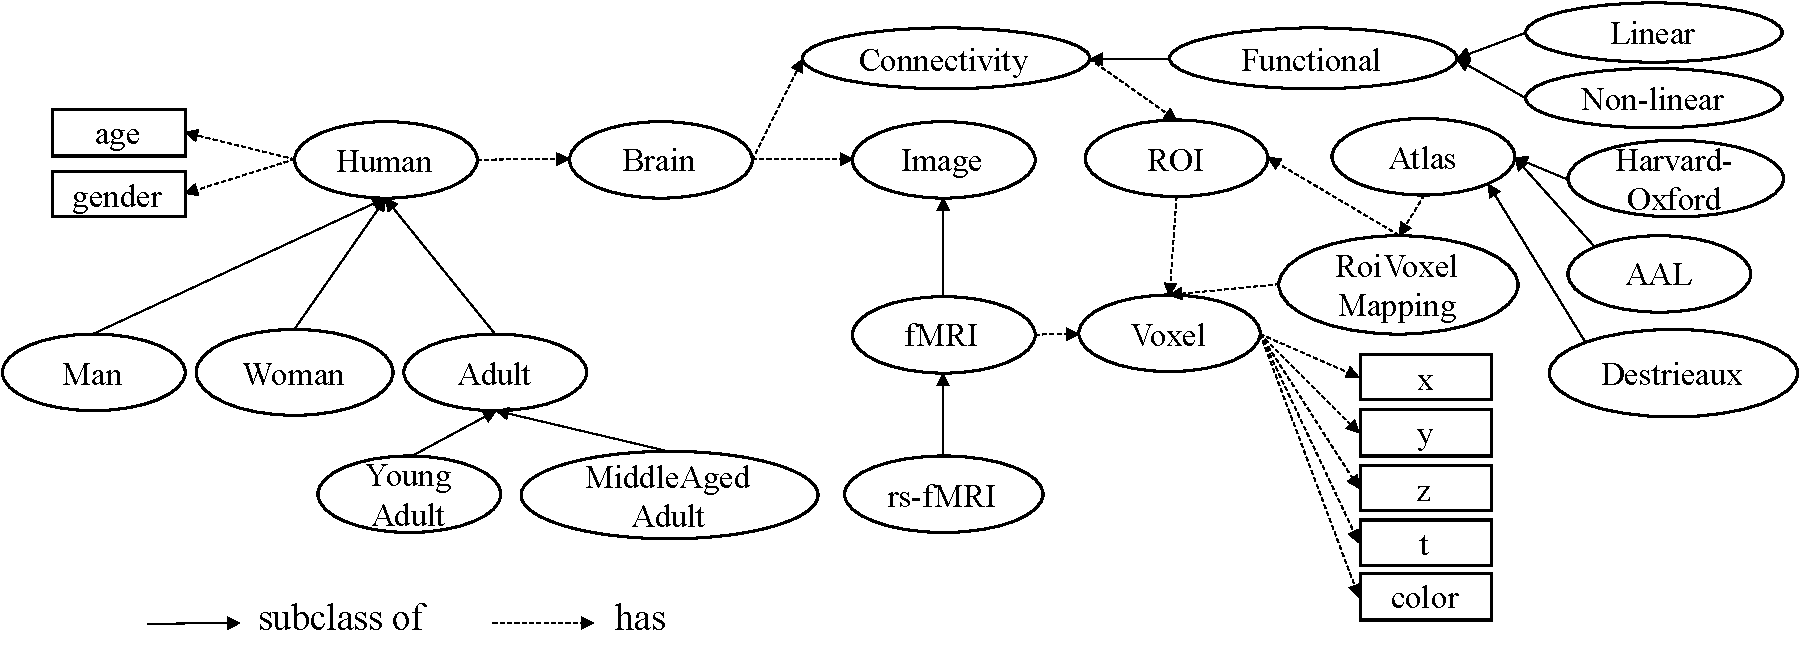
\includegraphics[width=1.0\linewidth]{images/DomainOnto.pdf}
    \caption{Воплощение гипотезы.}\label{fig:DomainOnto}
\end{figure}

Обычно онтологии предметной области могут быть намного больше по размеру и довольно сложны в эксплуатации. 
Преимущество их использования заключается в том, что они позволяют использовать движки логического вывода над ними. 
В онтологии предметной области есть основные понятия, такие как человек, мозг, изображение, атлас и т.д. Каждый класс 
является подклассом специального класса \textbf{Thing}. Простые свойства данных, такие как возраст, пол и 
пространственно-временные координаты, изображены в квадратах. OwlReady2 позволяет указать определение подкласса 
со следующей конструкцией, например, взрослый среднего возраста "--- это взрослый, возраст которого составляет от 
30 до 45 лет, является подклассом взрослого (подкласс человека, где определяются возрастные и гендерные 
функциональные свойства) и не связан с классом \textbf{YoungAdult}:

\begin{ListingEnv}[!h]% настройки floating аналогичны окружению figure
    \captiondelim{ } % разделитель идентификатора с номером от наименования
    \caption{Часть онтологии предметной области с использованием OwlReady2}\label{lst:ontology}
    % окружение учитывает пробелы и табуляции и применяет их в сответсвии с настройками
    \begin{lstlisting}[language={Python}]
    
    class Human(Thing): pass
    class has_age(Human >> int, DataProperty, 
                    FunctionalProperty): pass
    class has_gender(Human >> int, DataProperty, 
                    FunctionalProperty): pass

    class Adult(Human):
            equivalent_to = [Human & has_age > 18]
    class YoungAdult(Adult):
            equivalent_to = [Adult & has_age < 30]
    class MiddleAgedAdult(Adult):
            equivalent_to = [Adult & has_age >= 30 & 
                            has_age < 45]
                            
    AllDisjoint([YoungAdult, MiddleAgedAdult])
\end{lstlisting}
\end{ListingEnv}

Нейроизображение "--- 4-мерное изображение (серия 3-мерных изображений), отражающее распределение метаболической 
активности в разных областях мозга в разные промежутки времени. Область мозга представляет собой набор вокселов, 
отсортированных по определенному признаку. Чаще всего представляется в виде временных рядов. Воксель "--- это элемент 
трехмерного изображения, содержащий некоторое значение.

Связность мозга "--- структура анатомических связей, статистических зависимостей или причинно-следственных 
взаимодействий между отдельными единицами нервной системы мозга. Структурная связность относится к сети физических 
или структурных связей, связывающих наборы нейронов или нейронных элементов со структурными биофизическими 
особенностями. Функциональная связность "--- это статистический тип связи между анатомически несвязанными областями 
мозга, которые обладают общими функциональными свойствами. Эффективная связность "--- сочетание структурной и 
функциональной связности. Она описывает сети направлений одного нейронного элемента по отношению к другому.

ФМРТ в состоянии покоя - это нейронное изображение, полученное в результате эксперимента, когда испытуемый находился 
в состоянии покоя и не занимался активными задачами.

\section{Спецификации гипотез и моделей для задач нейроинформатики}\label{sect_5_2}

Следующим шагом является определение гипотез предметной области, моделей и сопоставления гипотез с моделями. 
Есть четыре гипотезы, которые уточняются. Первый описывает, как следует выделять регионы головного мозга (ROI). 
Три конкурирующие модели, которые используют три атласа, сопоставлены с этой первой гипотезой. 

Вторая конкретизированная гипотеза касается функциональной связности и того, как ROI взаимодействуют друг с другом. 
Конкурирующие модели здесь линейные и нелинейные. Уравнения не указаны, и флаг для их генерации 
установлен в значение \textit{true}. 

Третья и четвертая гипотезы касаются существования значительных различий в функциональной связности у 
мужчин и женщин или у взрослых молодого и среднего возраста. Две конкурирующие модели для обеих гипотез "--- это 
модели разности уравнений и графов. Гипотезы и модели изображены на \cref{fig:Hypothesis_lattice}.

\begin{figure}[ht]
    \centering
    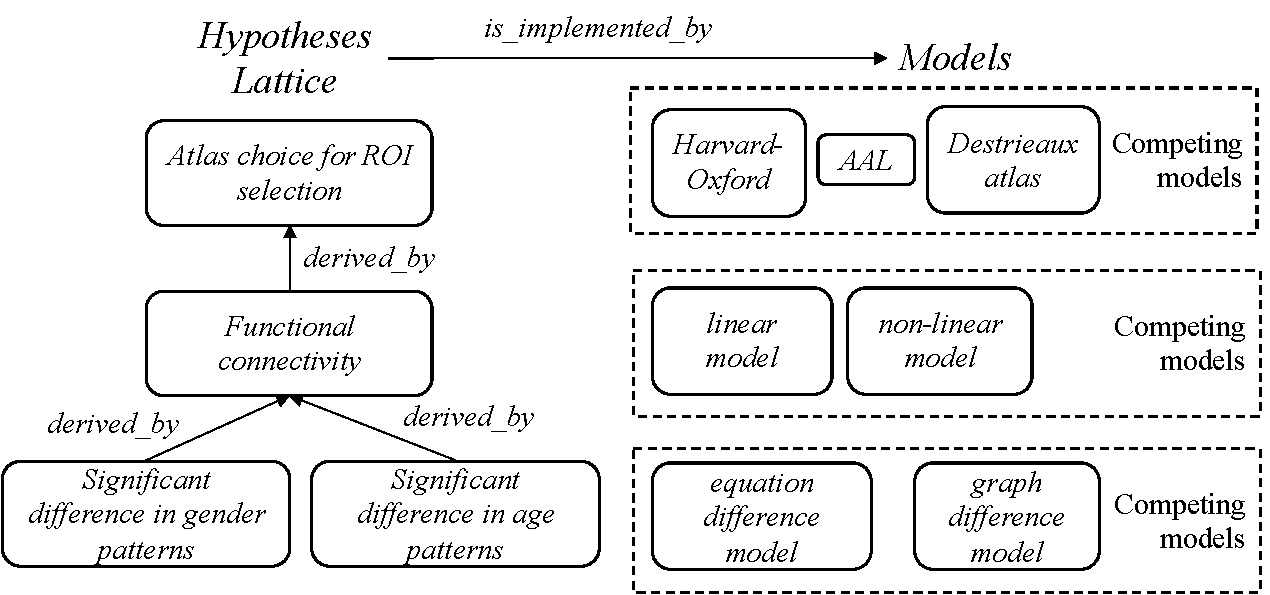
\includegraphics[width=1.0\linewidth]{images/Hypothesis_Lattice.pdf}
    \caption{Решетка гипотез для задач поиска различий в функциональной связности.}\label{fig:Hypothesis_lattice}
\end{figure}

Чтобы сгенерировать гипотезы на основе данных, требуется построить систему уравнений, описывающих функциональную 
взаимосвязь между несколькими переменными в наборе данных. Это не всегда необходимо в других областях, например, 
в астрономии теоретические уравнения известны заранее и их не нужно генерировать [10].
Для заявленной задачи нелинейные методы построения функциональных зависимостей позволяют построить большее 
количество моделей для более точного описания ожидаемых зависимостей [12]. Нелинейный подход заключается в построении 
нелинейной функции, которая выражает зависимость каждой отдельной переменной от других переменных. По умолчанию 
система использует генетическое программирование для построения нелинейных функций [13]. Это не требует 
каких-либо априорных предположений о зависимостях данных. Можно смешивать классы из онтологии домена с методами python. 
Для этого создается подкласс нелинейной модели из \textbf{Model} и добавляется метод \textit{fit} следующим образом:

\begin{ListingEnv}[!h]% настройки floating аналогичны окружению figure
    \captiondelim{ } % разделитель идентификатора с номером от наименования
    \caption{Определение нелинейной модели и ее метода \textit{fit}}\label{lst:fit}
    % окружение учитывает пробелы и табуляции и применяет их в сответсвии с настройками
    \begin{lstlisting}[language={Python}]
class NonLinearModel(Model):
    namespace = virtual_experiment_onto.
        get_namespace("http://synthesis.ipi.ac.ru/virtual_experiment.owl")

    def fit(self, X, y):
        est_gp = SymbolicRegressor(population_size=1000,
                                   tournament_size=20,
                                   generations=150, 
                                   stopping_criteria=0.001,
                                   const_range=(-1, 1),
                                   p_crossover=0.7, 
                                   p_subtree_mutation=0.12,
                                   p_hoist_mutation=0.06, 
                                   p_point_mutation=0.12,
                                   p_point_replace=1,
                                   init_depth=(6, 10),
                                   function_set=('mul', 'sub', 
                                         'div', 'add', 'cos'),
                                   max_samples=0.9,
                                   verbose=1,
                                   metric='mse',
                                   parsimony_coefficient=.005,
                                   random_state=0)

        est_gp.fit(X, y)
        return est_gp
\end{lstlisting}
\end{ListingEnv}

Подход к созданию моделей на основе данных использует общий метод линейной модели, основанный на данных. В результате 
таких комбинаций выбираются переменные, коэффициент для которых существенно отличается от нуля. Одновременно с 
общей линейной моделью для того же набора данных выполняется динамическое причинно-следственное моделирование. 
Комбинации выбранных переменных используются в качестве входных данных для метода генетического программирования. 
Использование такой эвристики может значительно сократить время работы генетического программирования, одновременно 
повышая точность соответствия данным наблюдений. Выходные системы уравнений ранжируются с использованием коэффициента 
детерминации; функция с наивысшим показателем возвращается эксперту.

\section{Сравнение конкурирующих гипотез для задачи поиска разности в 
            образцах функциональной связности у мужчин и женщин}

Результаты сравнения различных гипотез и соответствующих им моделей приводится для задачи поиска различий в 
функциональной связности у мужчин и женщин в состоянии покоя. Постановка и описание задачи приведены в 
\cref{sect_4_1}. Для поставленной задачи были сформулированы гипотезы и реализующие их 
модели (см.\cref{fig:Hypothesis_lattice}). Слева приведен граф зависимости нескольких гипотез между собой. 
Вершиной графа является набор конкурирующих между собой гипотез. Конкурирующими являются гипотезы, описывающие 
один и тот же феномен и реали-зованные различными вычислительными моделями. Приведенные методы сравнения работают 
для конкурирующих гипотез, для зависимых гипотез они не применимы.

Система поддержки виртуальных экспериментов автоматически вычисляет множество экспериментов, сочетающих разные 
конкурирующие гипотезы. Проведено четыре виртуальных эксперимента (атлас выбирается вручную), с использованием 
двух типов моделей "--- линейных и нелинейных и двух типов разностей предсказаний.

Для данной задачи выделены три множества конкурирующих гипотез: вы-бор атласов и выделение регионов головного 
мозга человека, построение функ-циональной связности регионов головного мозга, поиск значимых различий в 
функциональной связности у мужчин и женщин в состоянии покоя. Для первого множества нет единого способа выбрать 
ту или иную модель. В работе \cite{Arslan2018} сравнивается множество различных методов для выделения регионов. 
Они сравнивают их по 4 критериям, а именно: воспроизводимость, сохранение информации в связи со значительным 
уменьшением размерности, интерпретируемость. При этом отмечается, что модели не полностью сравнимы, поэтому 
окончательный выбор остается за экспертом в зависимости от решаемой задачи, набора данных и необходимости 
сравнения с другими работами. 

Для второго множества конкурирующих гипотез о функциональной связности регионов головного мозга используется несколько 
методов. Первым шагом для данного сравнения является отсечение моделей по пороговому значению коэффициента 
детерминации. Это делается для сокращения пространства сравниваемых моделей. Для 23 построены модели с оценкой 
выше порогового коэффициента детерминации, равным 0.7. Вторым шагом является сравнение линейных и нелинейных 
моделей, где нелинейные модели бы-ли получены методом генетического программирования, пример которых представлен ниже:

\begin{equation}
\begin{array}{l}
x_0 = \frac{\left(x_{43}-x_{41}\right) * (x_{13}-x_{26} )}{x_{26}} + x_{41}-x_3 \\
x_1= x_{39} * (0.756-x_{40})    
\end{array}
\end{equation}

Для сравнения используется критерии Акаике и Байеса по причине возможности сравнения моделей различной природы. 
Результаты сравнения с использованием информационного критерия Акаике приведены в \cref{tbl:aic_bic_gender}. Здесь 
и далее результаты приводятся только для регионов \textit{Precentual Gyrus}, \textit{Postcentral Gyrus} 
и \textit{Planum Polare}. Для критерия Акаике лучшей моделью является нелинейная модель, то время, как для 
критерия Байеса лучшей моделью оказалась линейная модель.

\begin{table} [ht]%
	\caption{Результаты сравнения моделей по информационным критериям}%
	\label{tbl:aic_bic_gender}% label всегда желательно идти после caption
    \setlength\extrarowheight{0pt} %вот этим управляем расстоянием между рядами, \arraystretch даёт неудачный результат
    \setlength{\tymin}{2.3cm}% минимальная ширина столбца
    \begin{center}

	\begin{tabulary}{\textwidth}{@{}>{\zz}L >{\zz}C >{\zz}C >{\zz}C >{\zz}C@{}}% Вертикальные полосы не используются 
        % принципиально, как и лишние горизонтальные (допускается по ГОСТ 2.105 пункт 4.4.5) % @{} позволяет 
        % прижиматься к краям
        \toprule     %%% верхняя линейка
    	  Регион &
    	AIC (линейная) &
            AIC (ГП) &
            BIC (линейная) &
            BIC (ГП) 
            \\
        \midrule %%% тонкий разделитель. Отделяет названия столбцов. Обязателен по ГОСТ 2.105 пункт 4.4.5 
        \textit{Precentual Gyrus} &
        -53\,058 &
        -58\,638 & 
        -54\,987 &
        -37\,821
        \\
        \midrule
        \textit{Postcentral Gyrus} &
        -46\,048 &
        -52\,315 & 
        -42\,874 &
        -34\,508  
        \\
        \midrule
        \textit{Planum Polare} &
        -7\,109 &
        -10\,658 & 
        -6\,925 &
        -3\,215    
        \\
        \bottomrule %%% нижняя линейка
	\end{tabulary}%
 \end{center}

\end{table}



Несоответствие между двумя информационными критериями вызвано тем, что в критерии Байеса учитывается не только точность 
предсказания, но также и сложность проверяемой модели. В модели генетического программирования число параметров 
значительно больше, чем в обычной линейной модели, поэтому у критерия Байеса оценка модели генетического 
программирования больше, чем у линейной. Если требуется не только точность предсказаний, но и простота модели, 
то следует использовать критерий Байеса, иначе критерий Акаике.

Третье множество конкурирующих гипотез о поиске значимых различий в функциональной связности у мужчин и женщин 
в состоянии покоя состоит из двух конкурирующих гипотез. Каждая из гипотез реализована следующими мо-делями. 
Первая модель представляет собой разность между предсказаниями для мужчин и женщин в выбранном регионе. Вторая 
модель строится вычитанием графов, построенных для мужчин и женщин, каждый из которых описывает взаимодействие 
между регионами головного мозга. Данные гипотезы не являются сравнимыми напрямую, а скорее являются взаимодополняющими. 
Если полу-ченные регионы со значимыми различиями не совпадают, то эксперту рекомендуется дополнительно проверить 
данный регион, например, используя другой набор данных.

Для первой модели проверяется равность медианы разности нулю с использованием статистического теста "--- критерия 
знаков \cite{pham2019new}, а также байесовского подхода. Результаты представлены в \cref{tbl:gp_2datasets} для 
трех регионов без потери наглядности.

\begin{table} [ht]%
	\caption{Результаты сравнения двух моделей генетического программирования, обученных на разных выборках}%
	\label{tbl:gp_2datasets}% label всегда желательно идти после caption
    \setlength\extrarowheight{0pt} %вот этим управляем расстоянием между рядами, \arraystretch даёт неудачный результат
    \setlength{\tymin}{2.3cm}% минимальная ширина столбца
    \begin{center}

	\begin{tabulary}{\textwidth}{@{}>{\zz}L >{\zz}C@{}}% Вертикальные полосы не используются принципиально, как и 
        % лишние горизонтальные (допускается по ГОСТ 2.105 пункт 4.4.5) % @{} позволяет прижиматься к краям
        \toprule     %%% верхняя линейка
    	  Регион &
    	Достигаемый уровень значимости 	\\
        \midrule %%% тонкий разделитель. Отделяет названия столбцов. Обязателен по ГОСТ 2.105 пункт 4.4.5 
        \textit{Precentual Gyrus} &
        0.0045 (отвергается) 
        \\
        \midrule
        \textit{Postcentral Gyrus} &
        0.0003 (отвергается)  
        \\
        \midrule
        \textit{Planum Polare} &
        0.08 (не отвергается)  
        \\
        \bottomrule %%% нижняя линейка
	\end{tabulary}%
 \end{center}

\end{table}

Уровень значимость выбран равным 0.05. Регионы \textit{Precentual Gyrus} и \textit{Postcentral Gyrus} являются 
различными для мужчин и женщин.  Для региона \textit{Planum Polare} нулевая гипотеза о схожести регионов 
не отвергается. Важным замечанием является то, что хотя нулевая гипотеза не отвергается, но полученное значение 
близко к порогу 0.05. Если выбрано значение порога, например, 0.1, то нулевая гипотеза о схожести региона 
отвергается для \textit{Planum Polare}. 

Результаты сравнения для байесовского подхода представлены в \cref{tbl:bayesian_gender}. Результаты совпадают 
с результатами для статистического теста. При этом появляется возможность оценить степень уверенности в результате. 

\begin{table} [ht]%
	\caption{Результаты сравнения байесовским подходом}%
	\label{tbl:bayesian_gender}% label всегда желательно идти после caption
    \setlength\extrarowheight{0pt} %вот этим управляем расстоянием между рядами, \arraystretch даёт неудачный результат
    \setlength{\tymin}{2.3cm}% минимальная ширина столбца
    \begin{center}

	\begin{tabulary}{\textwidth}{@{}>{\zz}L >{\zz}L >{\zz}C@{}}% 
        \toprule     %%% верхняя линейка
    	  Регион &
            $\eta$ &
    	Доказательная сила 	\\
        \midrule %%% тонкий разделитель. Отделяет названия столбцов. Обязателен по ГОСТ 2.105 пункт 4.4.5 
        \textit{Precentual Gyrus} &
        $29:1 (29)$ &
        Среднее доказательство 
        \\
        \midrule
        \textit{Postcentral Gyrus} &
        $54:1 (54)$ &
        Среднее доказательство  
        \\
        \midrule
        \textit{Planum Polare} &
        $7:1 (0.14)$ &
        Слабое доказательство
        \\
        \bottomrule %%% нижняя линейка
	\end{tabulary}%
 \end{center}

\end{table}

Для \textit{Precentual Gyrus} и \textit{Postcentral Gyrus} нулевая гипотеза схожести этих регионов у мужчин и 
женщин отвергается со средней степенью уверенности. При этом для \textit{Planum Polare} нулевая гипотеза не 
отвергается со слабой степенью уверенности, что говорит о необходимости дополнительного исследования данного 
региона. В целом результаты статистического и байесовского подхода схожи, но иногда они могут давать различные 
результаты. Для трех регионов было получено, что при использовании статистического теста регионы получились различны.

Другой предлагаемый метод сравнения гипотез основан поиска схожести графового представления соответствующих 
им моделей. На вход метод принимает теоретическую гипотезу в виде системы уравнений и набор данных, 
по которому будут сгенерированы конкурирующие гипотезы. По данным автоматически генерируются несколько 
конкурирующих гипотез. Производится вычисление для всех сгенерированных моделей выбранной экспертом 
метрики, отбирается одна лучшая гипотеза. Для обеих моделей, реализующих гипотезы 
(теоретическая гипотеза "--- построенная из данных гипотеза), строятся ориентированные ацикличные 
графы зависимости переменных из уравнений. Далее для пары графов выполняется сравнение их сходства 
посредством построения графа разности. Если для построенного графа его множество ребер не является 
пустым, то гипотезы считаются различными и возвращается истина, иначе возвращается ложь. 
Метод может быть применен, если модели представимы в виде ацикличных графов.

В качестве примера строится разность двух графов для мужчин и женщин \cref{fig:graph_difference}. 
Вершинами построенного графа разности являются регионы мозга, а ребрами "--- связи между регионами. Если 
функциональная связность региона является раз-личной у мужчин и женщин, то в графе разности 
присутствует хотя бы одно ребро для данного региона. Для полученного графа видно, что для регионов 
\textit{Postcentral Gyrus} и \textit{Planum Polare} получился такой же результат, как и в случае с 
использованием первой модели. Для региона \textit{Precentual Gyrus} результат отличается, 
т.~е. эксперту рекомендуется провести дополнительные исследования.


\begin{figure}[ht]
    \centering
    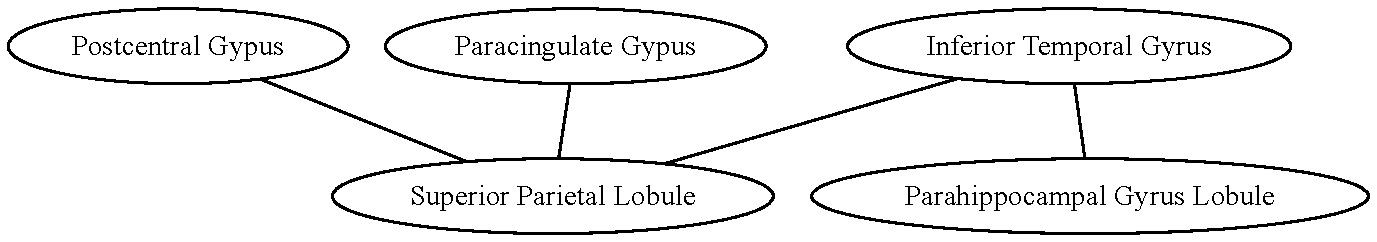
\includegraphics[width=1.0\linewidth]{images/graph_difference.pdf}
    \caption{Граф разности функциональной связности регионов для мужчин и женщин.}\label{fig:graph_difference}
\end{figure}

\section{Построение решетки гипотез}\label{sect_5_3}
Для работы с набором гипотез используется концепция решетки гипотез \cref{sect2_3}. Решетка используется 
для анализа того, какие части виртуального эксперимента необходимо пересчитать, а какие части можно 
загрузить из репозитория. Поток работ и его отображение в модели, реализованные на Python, 
изображены на \cref{fig:workflow}.

\begin{figure}[ht]
    \centering
    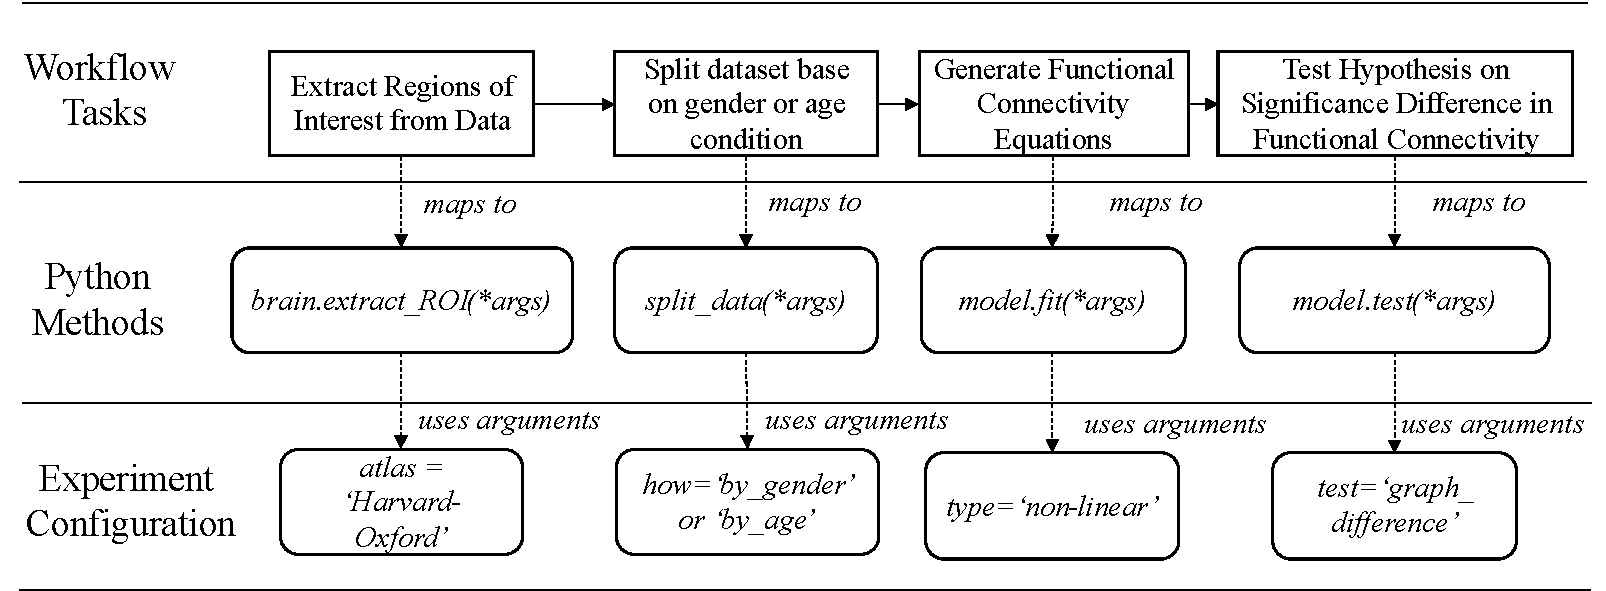
\includegraphics[width=1.0\linewidth]{images/Workflow_conf.pdf}
    \caption{Поток работ и конфигурация.}\label{fig:workflow}
\end{figure}

Параметры модели описаны в конфигурации. Извлечение ROI является общим шагом для обеих проблем. На этом 
этапе требуется преобразовать 4-мерное изображение мозга в двумерный массив (области мозга - время). 
Интересующие регионы группируются и усредняются некоторым образом, и само среднее значение является 
репрезентативным значением для данного региона. Самый популярный способ "--- использовать карты мозга - атласы. 
При работе с атласами человеческого мозга используется предварительно рассчитанная функция, которая присваивает 
каждому вокселу изображения некоторую область мозга.
Следующая задача потока работ "--- разделить набор данных по полу или возрасту. Выбор делается на основе 
конфигурации виртуального эксперимента. Третья задача "--- сгенерировать уравнения функциональной связности. 
Здесь могут быть использованы линейные и нелинейные модели. Эта задача реализуется компонентом генерации. 
Последняя задача "--- проверить гипотезу о наличии существенной разницы для обученных моделей.

\section{Выводы по главе}\label{sect4_3}


\clearpage           % Глава 4
\include{Dissertation/conclusion}      % Заключение
\include{Dissertation/acronyms}        % Список сокращений и условных обозначений
\chapter*{Словарь терминов}             % Заголовок
\addcontentsline{toc}{chapter}{Словарь терминов}  % Добавляем его в оглавление

\textbf{Научная гипотеза} : есть предлагаемое объяснение явления, которое еще должно быть подвергнуто строгой проверке 

\textbf{Научная теория} : уже прошла всесторонние испытания и широко принята в качестве точного объяснения, стоящего за наблюдением

\textbf{Научный закон} : это утверждение, которое показывает некоторую упорядоченность или регулярность в природе, существование неизменной связи между определенным комплексом условий и определенными явлениями

\textbf{Индукция} : сбор и интерпретация эмпирических доказательств. Это – методика, в которой собираются и рассматриваются разрозненные элементы доказательства до того момента, когда открывается закон или изобретается теория

\textbf{Научная теория} : обобщает гипотезу или группу гипотез, поддержанных неоднократными проверками. Теория справедлива, если нет ни одного противоречащего ей факта

\textbf{Научная парадигма} : объясняет рабочее множество теорий, на которых основана наука

\textbf{Решетка гипотез} : образуется при рассмотрении множества гипотез, расположенных в строгом порядке 

\textit{wasDerivedFrom} : была выведена из (снизу вверх). Гипотезы, непосредственно выведенные из одной-единственной гипотезы, называются атомарными, в то время как те, которые выведены, по крайней мере, из двух гипотез, называются комплексными

\textbf{Формульное моделирование} : это процесс оценки соотношений между переменными      % Словарь терминов
\include{Dissertation/references}      % Список литературы
\include{Dissertation/lists}           % Списки таблиц и изображений (иллюстративный материал)

\setcounter{totalchapter}{\value{chapter}} % Подсчёт количества глав

%%% Настройки для приложений
\appendix
% Оформление заголовков приложений ближе к ГОСТ:
\setlength{\midchapskip}{20pt}
\renewcommand*{\afterchapternum}{\par\nobreak\vskip \midchapskip}
\renewcommand\thechapter{\Asbuk{chapter}} % Чтобы приложения русскими буквами нумеровались

% \chapter{Свидетельство о государственной регистрации программы для ЭВМ}\label{app:A}

\refstepcounter{chapter}
\addcontentsline{toc}{appendix}{\protect\chapternumberline{\thechapter}Свидетельство о государственной регистрации программы для ЭВМ}\label{app:A}

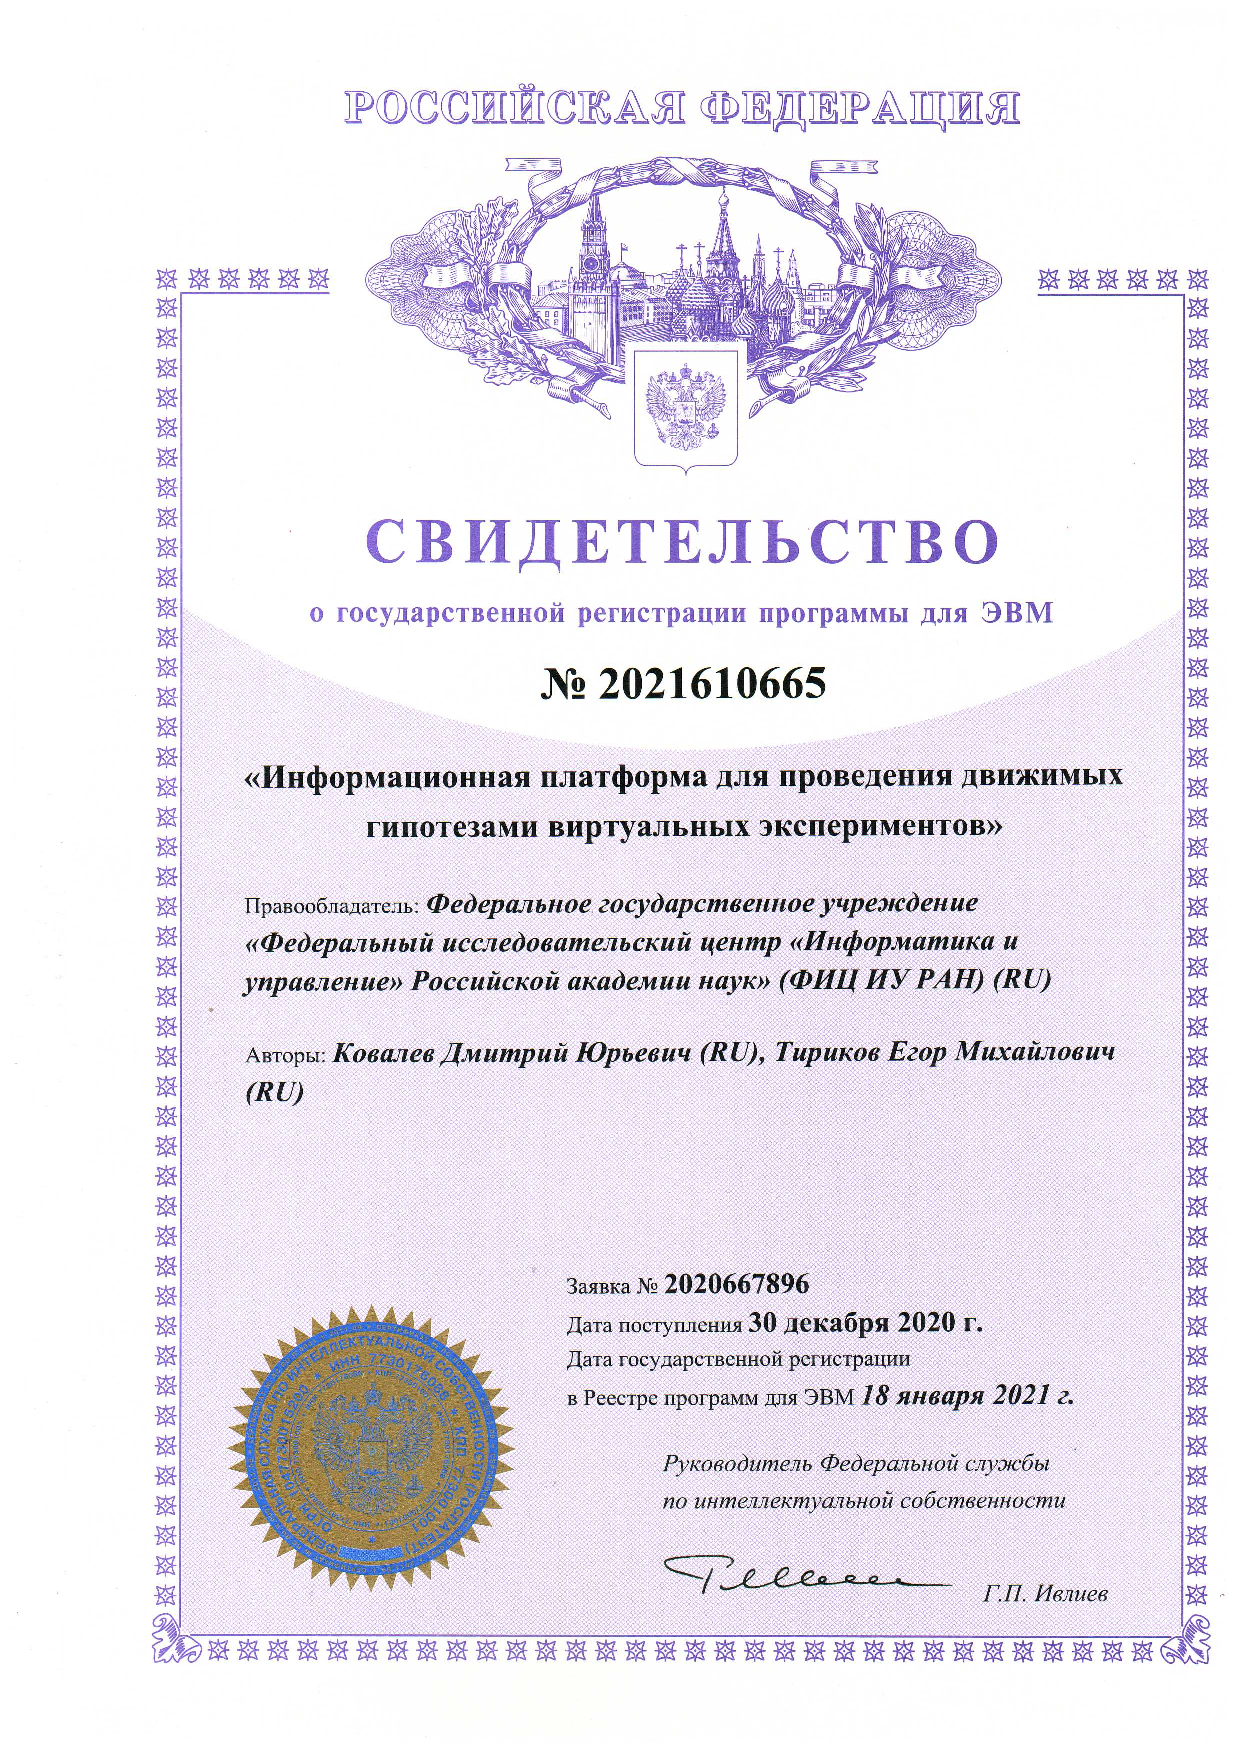
\includepdf[pages=-]{images/registration_program.pdf}
        % Приложения

\setcounter{totalappendix}{\value{chapter}} % Подсчёт количества приложений

\end{document}
